\documentclass[10pt]{report}


% Use the full page with 1 cm margins.

\usepackage[
  paper=letterpaper,
  nofoot,nomarginpar,
  includehead,
  margin=1cm
]{geometry}

% Use TeX Gyre Schola for text and math.

\usepackage[T1]{fontenc}
\usepackage{unicode-math}
\setmainfont{TeX Gyre Schola}
\setmathfont{TeX Gyre Schola Math}
\setsansfont{TeX Gyre Heros}

\usepackage{titlesec}
\usepackage{titletoc}
\usepackage{fancyhdr}
\usepackage{enumitem}
\usepackage{hyperref}
\usepackage{graphicx}
\usepackage{xcolor}
\usepackage{tabularx}
\usepackage{tabulary}
\usepackage{booktabs}
\usepackage{multicol}
\usepackage{microtype}
\usepackage{multirow}
\usepackage{pdflscape}

% Basic spacing.

\setlength{\columnsep}{2em}

\setlength{\parindent}{0em}
\setlength{\parskip}{0.8ex plus 0.1ex}
\newcommand{\numberspace}{\phantom{0}}

\newsavebox{\fitwidthbox}
\newenvironment{fitwidth}[1]{%
    \def\fitwidth{#1}%
    \begin{lrbox}{\fitwidthbox}%
}{%
    \end{lrbox}%
    \resizebox{\fitwidth}{!}{\usebox{\fitwidthbox}}%
}

% Headers

\newcommand{\therunningtitle}{}
\newcommand{\runningtitle}[1]{\renewcommand{\therunningtitle}{#1}}

\pagestyle{fancy}
\setlength{\headsep}{1em}
\fancyhead[L]{\textbf{\therunningtitle}}
\fancyhead[C]{}
\fancyhead[R]{\textbf{Page \thepage}}
\fancyfoot[L,C,R]{}
\setlength{\footskip}{4pt}
\renewcommand{\headruleskip}{0.1em}
\addtolength{\headheight}{\headruleskip}

% Line weights

\setlength{\arrayrulewidth}{0.4pt}
\setlength{\columnseprule}{0.4pt}
\renewcommand{\headrulewidth}{0.4pt}

% Lists

\setlist[itemize]{
  label=--,
  leftmargin=1.5em,
  rightmargin=1.5em,
  nosep,
  parsep=\parskip
}
\setlist[enumerate]{
  leftmargin=1.5em,
  rightmargin=1.5em,
  nosep,
  parsep=\parskip
}

\newcommand{\itemparagraph}[1]{{\bfseries #1}}

% Sections

\setcounter{secnumdepth}{3}

\newcommand{\beforesectionnumber}{}
\newcommand{\aftersectionnumber}{}
\newcommand{\beforesubsectionnumber}{}
\newcommand{\aftersubsectionnumber}{}
\newcommand{\beforesubsubsectionnumber}{}
\newcommand{\aftersubsubsectionnumber}{}

\titleformat{\section}
    [block]
    {\filcenter\large\bfseries}
    {\beforesectionnumber\thesection\aftersectionnumber}
    {\wordsep}
    {\MakeUppercase}
\titlespacing{\section}{0pt}{2.4ex plus .1ex minus .1ex}{1.3ex minus .1ex}

\titleformat{\subsection}
    {\filright\large\bfseries}
    {\beforesubsectionnumber\thesubsection\aftersubsectionnumber}
    {\wordsep}
    {}
\titlespacing{\subsection}{0pt}{1.8ex plus .1ex minus .1ex}{0.3ex minus .1ex}

\titleformat{\subsubsection}
    {\filright\bfseries}
    {\beforesubsubsectionnumber\thesubsubsection\aftersubsubsectionnumber}
    {\wordsep}
    {}
\titlespacing{\subsubsection}{0pt}{1.2ex plus .1ex minus .1ex}{0.3ex minus .1ex}

\newcommand{\afterparagraphtitle}{}
\titleformat{\paragraph}[runin]{\bfseries}{}{0.5em}{}[\afterparagraphtitle]
\titlespacing{\paragraph}{0em}{0em}{\wordsep}

\newcommand{\advancedrules}{
    \vspace{1ex}
    \pagebreak[1]
    \begin{center}
        \bfseries{\large Advanced Rules}
    \end{center}
}

\newcommand{\trainingnote}[1]{
  \vspace{1ex}
  \begin{center}
    \framebox{\begin{minipage}{0.9\linewidth} #1\end{minipage}}
  \end{center}
  \vspace{1ex}
}

% Style for the standard title page

\let\originaltitle\title
\renewcommand{\title}[1]{\originaltitle{\bfseries\Large\MakeUppercase{#1}}}
\let\originalauthor\author
\renewcommand{\author}[1]{\originalauthor{\itshape\normalsize{#1}}}
\let\originaldate\date
\renewcommand{\date}[1]{\originaldate{\normalsize{#1}}}

% Abbreviations

\newcommand{\AirSup}{\textit{Air Superiority}}
\newcommand{\AirStr}{\textit{Air Strike}}
\newcommand{\DF}{\textit{Desert Falcons}}
\newcommand{\EOTG}{\textit{Eagles of the Gulf}}
\newcommand{\TSOH}{\textit{The Speed of Heat}}
\newcommand{\AirPow}{\textit{Air Power}}
\newcommand{\APJ}{\textit{Air Power Journal}}

\newcommand{\FP}  {\text{FP}}
\newcommand{\FPs} {\text{FPs}}
\newcommand{\HFP} {\text{HFP}}
\newcommand{\HFPs}{\text{HFPs}}
\newcommand{\VFP} {\text{VFP}}
\newcommand{\VFPs}{\text{VFPs}}
\newcommand{\CC}  {\text{CC}}

\newcommand{\onethird}{$1/3$}
\newcommand{\onehalf}{$1/2$}
\newcommand{\twothirds}{$2/3$}

\renewcommand{\deg}{\ensuremath{^\circ}}


%%%%%%%%%%%%%%%%%%%%%%%%%%%%%%%%%%%%%%%%

% Aids.

% We use this flag to change formatting according to whether we are in
% the main text or the aids.

\newif\ifaids
\aidsfalse

%%%%%%%%%%%%%%%%%%%%%%%%%%%%%%%%%%%%%%%%

% Floats

\newenvironment{onecolumntable}[1][tp]{
    \begin{table}[#1]
    \ifaids
        \centering
        \begin{minipage}{0.5\linewidth}
    \fi
    \centering
    
}{
    \ifaids
        \end{minipage}
    \fi
    \end{table}
}

\newenvironment{twocolumntable}[1][tp]{
    \begin{table*}[#1]
    \centering
}{
    \end{table*}
}

\newenvironment{fullwidthtable}[1][tp]{
    \begin{table*}[#1]
    \centering
}{
    \end{table*}
}

\newenvironment{onecolumnfigure}[1][tp]{
    \begin{figure}[#1]
    \ifaids
        \centering
        \begin{minipage}{0.5\linewidth}
    \fi
    \centering
}{
    \ifaids
        \end{minipage}
    \fi
    \end{figure}
}

\newenvironment{twocolumnfigure}[1][tp]{
    \begin{figure*}[#1]
    \centering
}{
    \end{figure*}
}

% Align floats in their own page or column to the top.
\makeatletter
\setlength{\@fptop}{0pt}
\setlength{\@fpbot}{0pt plus 1fil}
\makeatother

%%%%%%%%%%%%%%%%%%%%%%%%%%%%%%%%%%%%%%%%

% Table and figure captions. 

% Some tables appear in both the main text
% and the play aids. Others only in the play aids.

\newcommand{\tablecaption}[2]{
    \ifaids
        \par
        {\normalsize Table~\ref{#1}: #2}
        \par
    \else
        \caption{\normalsize #2}
        \label{#1}
    \fi
    \medskip
}

\newcommand{\tablecaptionforaidsonly}[2]{
    \par
    \caption{#2}
    \label{#1}
    \medskip
}
\newcommand{\tablecaptioncontinued}[2]{
    \par
    Table~\ref{#1} (continued): #2
    \par
    \medskip
}

\newcommand{\figurecaption}[2]{
    \ifaids
        \par
        \medskip
        Figure~\ref{#1}: #2
    \else
        \caption{#2}
        \label{#1}
    \fi
}

%%%%%%%%%%%%%%%%%%%%%%%%%%%%%%%%%%%%%%%%

% Tables

\newcommand{\minitable}[3][c]{\begin{tabular}[#1]{@{}#2@{}}#3\end{tabular}}

\newcommand*\vertical{\rotatebox{90}}

% New tabularx columns

\newcolumntype{P}{X}%
\newcolumntype{L}{>{\raggedright\arraybackslash}X}%
\newcolumntype{R}{>{\raggedleft\arraybackslash}X}%
\newcolumntype{C}{>{\centering\arraybackslash}X}%
\newcolumntype{q}[1]{>{\centering\arraybackslash\hspace{0pt}}p{#1}}

\newenvironment{tablenote}[1]{%
    \tabularx{#1}{L}%
    \vspace{\parskip}%
}{%
    \endtabularx%
}

%%%%%%%%%%%%%%%%%%%%%%%%%%%%%%%%%%%%%%%%

% Figures

\usepackage{tikz}
\usetikzlibrary{calc}
\usetikzlibrary{arrows.meta}

\newenvironment{tikzfigure}[1]{%
    \begin{fitwidth}{#1}%
    \begin{tikzpicture}[>={Stealth[length=1.5mm,inset=0pt]}]%
    \scriptsize%
}{%
    \end{tikzpicture}%
    \end{fitwidth}%
}

\newcommand{\drawaircraftcounter}[5]{
    \begin{athex}{#1}{#2}
        \begin{scope}[rotate=#3-45]
            \draw[fill=white] (-0.3,-0.3) rectangle (0.3,0.3);
            \node [anchor=center, transform shape] {
                \includegraphics[angle=45,width=0.6cm]{plan-views/#4.png}
            };
            \node [anchor=south east,rotate=#3-45] at (+0.3,-0.3) {\tiny #5};
        \end{scope}
    \end{athex}
}

\newcommand{\drawdashedcounter}[3]{
    \begin{athex}{#1}{#2}
        \begin{scope}[rotate=#3-45]
            \draw[dashed,fill=white] (-0.3,-0.3) rectangle (0.3,0.3);
        \end{scope}
    \end{athex}
}

\newcommand{\drawarrowcounter}[3]{
    \begin{athex}{#1}{#2}
        \begin{scope}[rotate=#3-45]
            \draw[fill=white] (-0.3,-0.3) rectangle (0.3,0.3);
            \draw[very thick, ->] (-0.2,-0.2) -- (0.2,0.2);
        \end{scope}
    \end{athex}
}


% The number is sqrt(0.75) to three decimal places. It is the distance between column centers of a hex grid in which the difference between row centers is 1.0.
\newcommand{\hexxfactor}{0.866}

\newenvironment{athex}[3][]{
    \begin{scope}[shift={(#2*\hexxfactor,#3)},#1]
}{
    \end{scope}
}
\newcommand{\miniathex}[4][]{\begin{athex}[#1]{#2}{#3}#4\end{athex}}

\newcommand{\drawhex}[3][]{
    \begin{athex}{#2}{#3}
        \begin{scope}[xscale=\hexxfactor]
            \draw [color=black!50,#1] (+0.667,+0.000) -- (+0.333,+0.500) -- (-0.333,+0.500) -- (-0.667,+0.000) -- (-0.333,-0.500) -- (+0.333,-0.500) -- cycle;
        \end{scope}
    \end{athex}
}

\newcommand{\drawdottedhex}[3][]{
    \begin{athex}{#2}{#3}
        \begin{scope}[xscale=\hexxfactor,color=black!25,#1]
            \draw (+0.667,+0.000) -- (+0.333,+0.500) -- (-0.333,+0.500) -- (-0.667,+0.000) -- (-0.333,-0.500) -- (+0.333,-0.500) -- cycle;
        \end{scope}
        \begin{scope}[color=black!25,#1]
            \draw[fill]     (0,0) circle (0.02);
            \draw[fill]  (30:0.5) circle (0.02);
            \draw[fill]  (90:0.5) circle (0.02);
            \draw[fill] (150:0.5) circle (0.02);
            \draw[fill] (210:0.5) circle (0.02);
            \draw[fill] (270:0.5) circle (0.02);
            \draw[fill] (330:0.5) circle (0.02);
        \end{scope}
    \end{athex}
}

\newcommand{\drawpositions}[3][]{
    \begin{athex}{#2}{#3}
        \begin{scope}[color=black!25,#1]
            \draw[fill]     (0,0) circle (0.02);
            \draw[fill]  (30:0.5) circle (0.02);
            \draw[fill]  (90:0.5) circle (0.02);
            \draw[fill] (150:0.5) circle (0.02);
            \draw[fill] (210:0.5) circle (0.02);
            \draw[fill] (270:0.5) circle (0.02);
            \draw[fill] (330:0.5) circle (0.02);
        \end{scope}
    \end{athex}
}

\newcommand{\drawmegahex}[2]{
    \begin{athex}{#1}{#2}
        \begin{scope}[yscale=5,xscale=5*\hexxfactor,ultra thick,color=black!25]
            \draw (+0.667,+0.000) -- (+0.333,+0.500) -- (-0.333,+0.500) -- (-0.667,+0.000) -- (-0.333,-0.500) -- (+0.333,-0.500) -- cycle;
        \end{scope}
    \end{athex}
}

\newcommand{\cliphexgrid}[4]{
    \clip (#1*\hexxfactor-0.667*\hexxfactor,#2-0.5-0.01) rectangle (#3*\hexxfactor+0.667*\hexxfactor,#4+0.5+0.01);
}

\newcommand{\drawhexgrid}[4]{
    \cliphexgrid{#1}{#2}{#3}{#4}
    \foreach \x in {0,2,...,#3} {
        \foreach \y in {0,1,...,#4} {
            \miniathex{0.0}{0.0}{\drawhex{\x}{\y}}
        }
    }
    \foreach \x in {1,3,...,#3} {
        \foreach \y in {0,1,...,#4} {
            \miniathex{0.0}{0.5}{\drawhex{\x}{\y}}
        }
    }
}

\newcommand{\drawpositiongrid}[4]{
    \cliphexgrid{#1}{#2}{#3}{#4}
    \foreach \x in {0,2,...,#3} {
        \foreach \y in {0,1,...,#4} {
            \miniathex{0.0}{0.0}{\drawpositions{\x}{\y}}
            \miniathex{1.0}{0.5}{\drawpositions{\x}{\y}}
        }
    }
}

\newcommand{\drawdotathex}[3][]{
    \miniathex{#2}{#3}{\draw [fill,color=black,#1] circle (0.1);}
}

\newcommand{\drawpositionathex}[3][]{
    \miniathex{#2}{#3}{\draw [fill,color=black,#1] circle (0.02);}
}

\newlength{\standardhexwidth}
\setlength{\standardhexwidth}{8.3mm}
\usepackage{xstring}

\IfStrEq{\thisversion}{1A}{
    \newcommand{\earlierversion}{}
    \newcommand{\earlierversions}{}
}{}
\IfStrEq{\thisversion}{1B}{
    \newcommand{\earlierversion}{1A}
    \newcommand{\earlierversions}{1A}
}{}
\IfStrEq{\thisversion}{1C}{
    \newcommand{\earlierversion}{1B}
    \newcommand{\earlierversions}{1A1B}
}{}
\IfStrEq{\thisversion}{1D}{
    \newcommand{\earlierversion}{1C}
    \newcommand{\earlierversions}{1A1B1C}
}{}
\IfStrEq{\thisversion}{2A}{
    \newcommand{\earlierversion}{1C}
    \newcommand{\earlierversions}{1A1B1C1D}
}{}
\IfStrEq{\thisversion}{2B}{
    \newcommand{\earlierversion}{2A}
    \newcommand{\earlierversions}{1A1B1C1D2A}
}{}
\IfStrEq{\thisversion}{2C}{
    \newcommand{\earlierversion}{2B}
    \newcommand{\earlierversions}{1A1B1C1D2A2B}
}{}
\IfStrEq{\thisversion}{3A}{
    \newcommand{\earlierversion}{2C}
    \newcommand{\earlierversions}{1A1B1C1D2A2B2C}
}{}

% These commands compare their first argument to \thisversion. If their first argument is an equal to, earlier than, or later than \thisversion, they evaluate their second argument. The first argument will normally be the version in which a change was made. The commands should be read as "if the change was made in this, in an earlier, or in a later version, then evaluate the second argument."

\newcommand{\ifthisversion}[2]{\IfStrEq{\thisversion}{#1}{#2}{}}
\newcommand{\ifearlierversion}[2]{\IfSubStr{\earlierversions}{#1}{#2}{}}
\newcommand{\iflaterversion}[2]{\IfSubStr{\earlierversions\thisversion}{#1}{}{#2}}

\newcommand{\textadded}[1]{\textcolor{blue}{#1}}
\newcommand{\textdeleted}[1]{\textcolor{red}{#1}}
\newcommand{\textnote}[1]{\textcolor{orange}{[#1]}}

\newcommand{\added}[1]{{\color{blue}#1}}
\newcommand{\deleted}[1]{{\color{red}#1}}
\newcommand{\note}[1]{{\color{orange}[#1]}}

\IfSubStr{\thissubversion}{Changes}{
    \newcommand{\addedin}[3]{%
        \ifthisversion{#1}{\added{#3}\endnote{Added in #2.}}%
        \ifearlierversion{#1}{#3}%
    }
    \newcommand{\textaddedin}[3]{%
        \ifthisversion{#1}{\textadded{#3}\endnote{Added in #2.}}%
        \ifearlierversion{#1}{#3}%
    }
    \newcommand{\deletedin}[3]{%
        \iflaterversion{#1}{#3}%
        \ifthisversion{#1}{\deleted{#3}\endnote{Deleted in #2.}}%
    }
    \newcommand{\textdeletedin}[3]{%
        \iflaterversion{#1}{#3}%
        \ifthisversion{#1}{\textdeleted{#3}\endnote{Deleted in #2.}}%
    }
    \newcommand{\changedin}[4]{%
        \iflaterversion{#1}{#3}%
        \ifthisversion{#1}{\deleted{#3} \added{#4}\endnote{Changed in #2.}}%
        \ifearlierversion{#1}{#4}%
    }
    \newcommand{\textchangedin}[4]{%
        \iflaterversion{#1}{#3}%
        \ifthisversion{#1}{\textdeleted{#3} \textadded{#4}\endnote{Changed in #2.}}%
        \ifearlierversion{#1}{#4}%
    }
    \newcommand{\notein}[2]{%
        \ifthisversion{#1}{\endnote{Note in #1: #2}}%
    }
    \newcommand{\itemaddedin}[3]{%
        \ifthisversion{#1}{\added{\item \added{#3}\endnote{Added in #2.}}}%
        \ifearlierversion{#1}{\item #3}%
    }
    \newcommand{\itemdeletedin}[3]{%
        \ifthisversion{#1}{\deleted{\item \deleted{#3}\endnote{Deleted in #2.}}}%
        \iflaterversion{#1}{\item #3}%
    }
    \newcommand{\tablerowaddedin}[3]{%
        \ifthisversion{#1}{#3\\}%
        \ifearlierversion{#1}{#3\\}%
    }
    \newcommand{\tablerowdeletedin}[3]{%
        \iflaterversion{#1}{#3\\}%
        \ifthisversion{#1}{#3\\}%
    }
}{
    \newcommand{\addedin}[3]{%
        \ifthisversion{#1}{#3}%
        \ifearlierversion{#1}{#3}%
    }
    \newcommand{\textaddedin}[3]{\addedin{#1}{#2}{#3}}
    \newcommand{\deletedin}[3]{%
        \iflaterversion{#1}{#3}%
    }
    \newcommand{\textdeletedin}[3]{\deletedin{#1}{#2}{#3}}
    \newcommand{\changedin}[4]{%
        \deletedin{#1}{#2}{#3}\addedin{#1}{#2}{#4}%
    }
    \newcommand{\textchangedin}[4]{\changedin{#1}{#2}{#3}{#4}}
    \newcommand{\notein}[2]{%
    }
    \newcommand{\itemaddedin}[3]{%
        \ifthisversion{#1}{\item #3}%
        \ifearlierversion{#1}{\item #3}%
    }
    \newcommand{\itemdeletedin}[3]{%
        \iflaterversion{#1}{\item #3}%
    }
    \newcommand{\tablerowaddedin}[3]{%
        \ifthisversion{#1}{#3\\}%
        \ifearlierversion{#1}{#3\\}%
    }
    \newcommand{\tablerowdeletedin}[3]{%
        \iflaterversion{#1}{#3\\}%
    }
}

\newcommand{\silentlydeletedin}[3]{%
    \iflaterversion{#1}{#3}%
}
\newcommand{\silentlyaddedin}[3]{%
    \ifthisversion{#1}{#3}%
    \ifearlierversion{#1}{#3}%
}
\newcommand{\silentlychangedin}[4]{%
    \iflaterversion{#1}{#3}%
    \ifthisversion{#1}{#4}%
    \ifearlierversion{#1}{#4}%
}

\newcommand{\CX}[3][2C-editing]{\changedin{2C}{#1}{#2}{#3}}
\newcommand{\AX}[2][2C-editing]{\addedin{2C}{#1}{#2}}
\newcommand{\DX}[2][2C-editing]{\deletedin{2C}{#1}{#2}}
\newcommand{\SAX}[2][2C-editing]{\silentlyaddedin{2C}{#1}{#2}}
\newcommand{\IAX}[2][2C-editing]{\itemaddedin{2C}{#1}{#2}}

\newcommand{\CY}[3][3A]{\changedin{3A}{#1}{#2}{#3}}
\newcommand{\AY}[2][3A]{\addedin{3A}{#1}{#2}}
\newcommand{\DY}[2][3A]{\deletedin{3A}{#1}{#2}}
\newcommand{\SAY}[2][3A]{\silentlyaddedin{3A}{#1}{#2}}
\newcommand{\IAY}[2][3A]{\itemaddedin{3A}{#1}{#2}}
\newcommand{\IDY}[2][3A]{\itemdeletedin{3A}{#1}{#2}}

\newcommand{\CXY}[3]{\CX{#1}{\CY{#2}{#3}}}



\runningtitle{Air Power Rules (\thisversion\thissubversion)}

\begin{document}

\thispagestyle{empty}

\begin{minipage}{\linewidth}
%\vspace{1ex}
\begin{center}
{\LARGE \textbf{AIR POWER}}\\
\vspace{3ex}
Version \thisversion\\[\smallskipamount]
Revision \thisrevision\\
\vspace{3ex}
\textbf{“FIGHT TO FLY, FLY TO FIGHT, FIGHT TO WIN!”}\\
\vspace{1ex}
Motto of the U.S. Navy Fighter Weapons School\\
\vspace{1ex}
“Top Gun”
\end{center}
\vspace{1ex}
\end{minipage}

\begin{multicols}{2}

\begin{center}
\textbf{DEDICATION}
\end{center}

To all those who so patiently awaited this and especially to Rex “Van” Vandeboe, a good friend who tragically died of a heart attack at age 36. Truly a great guy, and a fun competitive gamer who was among the best I ever matched wits with. Van; this one’s for you bud.

\begin{center}
\textbf{CREDITS}
\end{center}

\begin{tabular}{@{}p{4cm}p{4cm}}
Research and Design: &J.D. Webster\\
Design Assistance:   &Mark Bovankovich\\
                     &Tom Phillips\\
                     &Rob Pruden\\
                     &Tony Valle\\
Typesetting:         &J.D. Webster\\
                     &Phil Boinske\\
\end{tabular}

\begin{center}
\textbf{PLAYTESTERS}
\end{center}

Jim Barrow, Bill Bishop, Scott Bogdan, Phil Boinske, Scott Brown, Pat Bryant, Steve Bush, Mike Dernoga, Dave Fiorito, Dan Foxman, Scott Genung, Mike Gingold, Bob Gross, Stora Harris, Mark Howell, Fran Kiger, Kevin Larabee, Steve Madjanovich, Curtis Maki, John Metcalf, Karl Mueller, Pat Passe, Gary Pilkington, Steve Paul, Paul Procyk, Arin Schonbach, Tim Tynan, David Van Bibber, Jeremy Van Bibber, Eric Van Bibber, Bill Van Slyke, Rex Vandeboe, Lee Brimmicombe-Wood, Joel Williams and Alan Wilmot.

(Thanks, guys, you did a great job! Sorry if I missed anyone.)

\begin{center}
\textbf{ADDITIONAL CREDITS}
\end{center}

\begin{tabular}{@{}p{4cm}p{4cm}}
\silentlyaddedin{1A}{Second Edition Editor:     &Malcolm Pipes\\}
\silentlyaddedin{1B}{Version 1B Errata:         &J.D. Webster\\}
\silentlyaddedin{1B}{                           &Felix Hack\\}
\silentlyaddedin{1B}{Version 1B Contributors:   &Karl Mueller\\}
\silentlyaddedin{1B}{&John Caraher\\}
\silentlyaddedin{1B}{&Felix Hack\\}
\silentlyaddedin{1B}{&Guy Alcala\\}
\silentlyaddedin{1B}{&Ethan Mckinney\\}
\silentlyaddedin{1B}{&Rob Pruden\\}
\silentlyaddedin{1B}{&Lee Brimmicombe-Wood\\}
\silentlyaddedin{1B}{&Chris Perlsberg\\}
\silentlyaddedin{1B}{&Mark Bovankovich\\}
Typesetting and Editing:    &Alan Watson Forster\\
\end{tabular}

\vfill\null\columnbreak

\setcounter{tocdepth}{1}
\begin{center}
\textbf{CONTENTS}
\end{center}
\contentsmargin{2em}
\dottedcontents{section}[2em]{}{2em}{0.5em}
\renewcommand\contentsname{}
\begingroup
\let\clearpage\relax
\vspace{-2cm}
\tableofcontents
\endgroup

\end{multicols}

\twocolumn
\rulechapter{In This Game}

This rule introduces the {\AirPow} game system and its components.


\CX{

\section{The Game System}

The {\AirPow} game system allows you to control one or more jet fighters in scenarios reflecting the actual life and death situations faced by fighter pilots in modern air combat. These rules provide the procedures for simulating jet fighter combat on a game board. As players, you must provide the brains, the strategy, and the tactics that will allow your jets to survive combat and win the various game scenarios.

Note: The {\AirPow} system is a derivative of the game system I used in GDW’s {\AirSup} and {\AirStr} games (now out of print), and as a result the data cards and most of the information tables used in the {\AirSup} games are fully compatible with this game system and may be used with it.

}{

\section{Game System}

The {\AirPow} game system allows you to control one or more jet fighters in scenarios reflecting the life-and-death situations fighter pilots faced in air combat historically since 1950 and continue to face in the present day. These rules provide the procedures for simulating jet fighter combat on a game board. As players, you must provide the brains, the strategy, and the tactics that will allow your jets to survive combat and win the various game scenarios.

The {\AirPow} system is a derivative of the game system used in GDW’s {\AirSup} and {\AirStr} games and Clash of Arms’ {\TSOH} game (now all out of print). As a result, the aircraft data cards and most of the weapons data tables from those games can be adapted to this game system and used with it.

}

\section{Game Scale}

\AX{
The scales in the game are as follows:
}

\begin{itemize}
    \item Each game turn represents 12 seconds of real time.
    \item Each map hex covers a distance of {\onethird} \CX{a}{of a} statute mile\AX{\ or 1,760 feet}.
    \item Each altitude level represents 1,000 feet of height.
    \item Each altitude band \addedin{1B}{1B-apj-23-errata}{typically }is 8,000 to 10,000 feet thick.
    \item Each aircraft speed point equals 100 mph of speed.
    \item Each aircraft counter represents a single \CX{jet}{aircraft}.
    \itemaddedin{2B}{2B-missile-counters}{Each missile counter represents a single missile.}
\end{itemize}

\AX{
The length of the game turn fixes the relation in the game between aircraft speed and distance moved. In 12 seconds, a real aircraft moving in level flight at 100~mph will move $1/3$ of a mile (100 miles per hour divided by 3600 seconds per hour multiplied by 12 seconds is $1/3$ of a mile). Similarly, in the game an aircraft moving in level flight at a speed of 1.0 (equivalent to 100~mph) will move 1 hex (equivalent to $1/3$ of a mile).
}

\DY{

\section{Learning the Game System}

\CX{

\paragraph{Read The Basic Rules First.} You should read only the rules that appear before any “Advanced Rules” header within each chapter. Skip the advanced rules and read on into the next chapter. Keep reading until you are instructed to play a Training Scenario. Take a break, then set up the scenario, and play it out. All of the Training Scenarios are designed for solitaire play. When you have finished, return to where you left off and continue reading. Do this until you’ve been exposed to all the basic rules and played all training scenarios.

\paragraph{Read the Advanced Rules If Desired.} Advanced rules are optional in nature and allow you to raise the level of detail and realism contained in the game. Using the advanced rules will increase the complexity of play but rewards you with a more accurate depiction of modern air combat. All, some, or none of the advanced rules may be learned and used as agreed upon by the players. The training scenarios may be replayed with advanced rules for practice.

\paragraph{Be Patient and Have Fun!} Don’t expect to learn all the rules in a single \CX{seating}{sitting}. Take your time and enjoy yourself. After playing several of the training scenarios, you will begin to get the hang of the system. Don’t forget, this is a game. Play it for its entertainment value, and have a good time as you strive to master the intricacies of modern air combat.

}{

\paragraph{Read The Basic Rules First.} You should read only the basic rules before any “Advanced Rules” header within each chapter. Skip the advanced rules and keep reading the basic rules until you are instructed to play a training scenario. Take a break, set up the scenario, and play it out. All of the training scenarios are designed for solitaire play. When you have finished, return to where you left off and continue reading. Do this until you’ve been exposed to all the basic rules and played all the training scenarios.

\paragraph{Read the Advanced Rules If Desired.} Advanced rules are optional and allow you to raise the level of detail and realism in the game. Using the advanced rules will increase the complexity of play but will reward you with a more accurate depiction of modern air combat. All, some, or none of the advanced rules may be used as agreed upon by the players. You may replay the training scenarios with advanced rules for practice.

\paragraph{Be Patient and Have Fun!} Don’t expect to learn all the rules in a single sitting. Take your time and enjoy yourself. After playing several training scenarios, you will begin to get the hang of the system. Don’t forget, this is a game. Play it for its entertainment value, and have a good time as you strive to master the intricacies of modern air combat.

}

}

\section{Game Components}

\CX{

Like most simulation games, those in this system have the following basic types of components:

\paragraph{1. Game Rules.} This set of rules defines how aircraft, missiles, and ground units move, detect enemies, and fight. It is not necessary to memorize the rules. Play aid sheets summarizing the key points of the rules are provided.

Once familiar with the rules, you should be able to play the game referring to the play aid charts alone; returning to the rules booklet only to clarify questions. There are two different levels of rules: Basic, and Advanced. Basic rules are all that are necessary to play any scenario in the game.

\paragraph{2. Game Charts.} Game charts distill large amounts of information into easily used tables. Players use the charts to determine specific capabilities of their aircraft and weapons, and to resolve combat. Charts in this system include: Flight and combat rules summaries, weapons data tables, aircraft data cards, and aircraft logsheets.

\paragraph{3. Game Counters.} The die-cut cardboard counters are the game pieces used to represent the aircraft, missiles, and ground units involved in play. Some of the counters represent information (such as target hits) rather than objects. Usually less than 20 pieces will be required for the play of any scenario. The counters shown \changedin{1C}{1C-figures}{here}{in Figure~\ref{figure:game-counters}} represent a fighter and an air to air missile. Each has a distinctive silhouette and color scheme that lets players recognize them easily.

\paragraph{4. Dice.} Each game in this system includes one ten-sided die as a random number generator. {\AirPow} uses the die to resolve events of chance during play. The die is marked with ten digits: 0 to 9. When rolled, it produces numbers from 0 to 9; the topmost number on the die is the one read. The 0 is always read as a 10. Thus, when the ten-sided die is rolled, it will produce a number from 1 to 10.

Die usage example: if a game chart indicates that a certain missile will hit its target 80\% of the time when it attacks. A player must use the die and roll 8 or less in order to hit. That die roll represents the 80\% probability of hitting. In this case, a miss would occur if a 9 or 10 was rolled.

\paragraph{5. Game Maps.} The game maps are the surface over which the playing pieces will be moved. Though several are provided, sometimes only a few will be used in a scenario. The hexagon grid on each map provides spaces in which players place and move their counters. Like a chessboard, the hexagons help to clearly define where a counter is. Distance between counters (range) is determined by counting the number of hexes between them. \addedin{1B}{1B-apj-23-errata}{Altitude differences may affect range calculations.}

For example, \changedin{1C}{1C-figures}{as}{Figure~\ref{figure:game-map} shows two game counters on a game map. As} each hex represents {\onethird} of a mile of distance, and as the two aircraft counters shown\deletedin{1C}{1C-figures}{ in the diagram below} are 6 hexes apart horizontally, they are a scale two miles apart. 
\deletedin{1C}{1C-figures}{\addedin{1B}{1B-apj-23-errata}{[The two aircraft counters were left off the diagram.]}}
Notice the large shaded hex outlines on the map. These are termed “megahexes”. Each megahex is 5 regular hexes across and allows players to determine long ranges and distances easier by counting in fives. 

}{

Games in this system have the following components:

\paragraph{Game Rules.} These rules define how aircraft, missiles, and ground units move, detect enemies, and fight. It is not necessary to memorize the rules. \DY{There are two different levels of rules: basic and advanced. Basic rules are all that are necessary to play any scenario in the game.}

\paragraph{Game Tables and Figures.} The tables present large amounts of information in a compact form. The figures show spatial relations. Once familiar with the rules, you should be able to play the game by referring to the play-aids alone, returning to the text of the rules only to clarify doubts.

\paragraph{Aircraft Data Cards and Weapon Data Tables.} The aircraft data cards present the flight and combat capabilities of the aircraft in terms of the game rules and are described in more detail in Rule~\ref{rule:aircraft-data-cards}. The weapon data tables give the combat capabilities of air-to-air, air-to-ground, and ground-to-air weapons.

\paragraph{Game Counters.} Some of the die-cut cardboard counters are used to represent elements such as aircraft, missiles,  ground units, and naval units. Other counters represent information such as target hits. Usually, less than 20 counters are required to play a scenario. The game counters shown in Figure~\ref{figure:game-counters} represent a fighter and an air-to-air missile. Each has a distinctive silhouette and color scheme, allowing players to recognize it easily.

\paragraph{Game Maps.} The game maps are the surface over which the counters are moved. Though several are provided, sometimes only a few will be used in a scenario. The hexagon grid (“hex grid”) on the maps provides spaces in which players place and move their game counters. Like a chessboard, the hexagons clearly define the position of a counter.

For example, Figure~\ref{figure:game-map} shows two game counters on a game map. Since each hex represents {\onethird} of a mile and as the two aircraft counters shown are six hexes apart horizontally, they are a scale two miles apart. Notice the large shaded hex outlines on the map. These are termed “megahexes”. Each megahex is five regular hexes across, allowing players to determine long horizontal distances more easily by counting in fives.

\paragraph{Aircraft Log Sheets.} The aircraft log sheets are used to record the speed and altitude of the aircraft and to help determine the changes in these as they maneuvers. A pad of generic aircraft log sheets is provided with each game. One log should be used for each aircraft in play. You may make copies of the sheets. The use of the log sheets is described in more detail in rule~\ref{rule:aircraft-log-sheets}.

\paragraph{Die.} The game system uses a ten-sided die to resolve events of chance during play. The die is marked with the digits 0 to 9. When rolled, the topmost number on the die is the one read, and 0 is always read as a 10. Thus, each die roll produces a number from 1 to 10.

The rules often state that the die roll should be modified under certain circumstances. For example, the rules may state that if a certain condition is fulfilled, the die roll should be modified by $+2$. In this case, if the condition is fulfilled, two should be added to the die roll's result, producing a number from 3 to 12.

The results of die rolls are typically used in one of two ways. If the die roll is to determine success or failure, the die roll result for success is given as a number or less. For example, if the rules state that success occurs on a die roll of $6-$, then success will occur if the modified die roll result is six or less. In the absence of modifiers, this corresponds to a 60\% chance of success. If the die roll is to determine which of several events occur, then a range of die roll results will be given for each event. For example, $1-$ (one or less) for outcome A, 2--7 (two to seven) for outcome B, and $8+$ (eight or more) for outcome C.


}

\changedin{1C}{AWF}{

\begin{FIGURE}[h!]
\includegraphics[width=\linewidth]{figures/figure-game-counters.pdf}
\end{FIGURE}

}{

\begin{FIGURE}[tp]

\includegraphics[width=1.5cm]{figures/counter-f-4.jpg}
\hspace{1.5cm}
\includegraphics[width=1.5cm]{figures/counter-aam.jpg}

\CAPTION{figure:game-counters}{\protect\x{Game Counters}{The game counter on the left represents an F-4 Phantom II and the one on the right an air-to-air missile.}}

\end{FIGURE}

}



\begin{tikzfigure}{\linewidth}
    \drawhexgrid{0}{0}{16}{12}
    \drawmegahex{3}{-1.5}
    \drawmegahex{3}{+3.5}
    \drawmegahex{3}{+8.5}
    \drawmegahex{3}{+13.5}
    \drawmegahex{8}{+6.0}
    \drawmegahex{8}{+11.0}
    \drawmegahex{8}{+16.0}
    \drawmegahex{13}{-1.5}
    \drawmegahex{13}{+3.5}
    \drawmegahex{13}{+8.5}
    \drawmegahex{13}{+13.5}
    \drawhexgrid{0}{0}{16}{+12}
    \drawaircraftcounter{10}{10}{60}{MiG-21}{B}
    \drawaircraftcounter{7}{5.5}{30}{F-4}{A}
\end{tikzfigure}


\rulechapter{The Game Turn}

This chapter describes game turns and how they are divided into phases to regulate play.

In {\AirPow}, a scenario is played out in game turns (often just called turns). Each game turn represents 12 seconds of real time.  A game turn is a tool used to regularize the movement and combat actions of the playing pieces. Within each turn, all aircraft and weapons in flight will get to move a scale distance equal to that which could be moved in 12 seconds of real time.

\section{Phases Within A Turn}
\label{rule:phases}

More than movement takes place in a turn. Air combat is a confusing affair in which opposing pilots are hotly engaged in sorting, tracking and attacking their enemies. This all happens in a continuous, rapid, dynamic and fluid manner. To keep the game manageable, the various actions pilots are concerned with, such as sighting the enemy or using radar etc., have been defined and given specific times during the game turn, called “phases”, in which they will be attended to. Each aircraft in play may participate in each phase dependent on the ability of the aircraft to function in those phases (i.e., an aircraft without a radar, would not participate in the radar phase). The order in which the phases are accomplished is termed the “Sequence of Play” (SOP).

The {\AirPow} SOP is shown \changedin{1C}{1C-tables}{below}{in Table~\ref{table:sequence-of-play}} and must be followed exactly in each game turn. However, phases which are not applicable to the scenario or current situation can be skipped over to speed play. Often, the scenarios are simply air combat ones not involving ground units. In those scenarios, the AAA, SAM, and Ground Unit interaction phases can be ignored.

\begin{onecolumntable}
\tablecaption{table:sequence-of-play}{Sequence of Play}
\begin{tabularx}{0.8\linewidth}{X}
\toprule
\x{
\begin{enumerate}
    \item AAA Interaction Phase.
    \item SAM Interaction Phase.
    \item Stalled Aircraft Phase.
    \item Visual Sighting Phase.
    \item Aircraft Decisions Phase.
    \item Order of Flight Determination Phase.
    \item Flight Phase.
    \item Air To Air Missile Phase.
    \item Air Radar Lock-on Phase.
    \item Ground Unit Interaction Phase.
    \item Aircraft Admin Phase.
    \item End of Turn Admin Phase.
\end{enumerate}
}{
\begin{enumerate}
    \item AAA interaction phase
    \item SAM interaction phase
    \item Stalled aircraft phase
    \item Visual sighting phase
    \item Aircraft decisions phase
    \item Order-of-flight determination phase
    \item Flight phase
    \item Air-to-air missile phase
    \item Air radar lock-on phase
    \item Ground unit interaction phase
    \item Aircraft administration phase
    \item End-of-turn administration phase
\end{enumerate}

}
\\
\bottomrule
\end{tabularx}
\end{onecolumntable}


There are reasons for the specific order of the phases. Visual sighting comes before the flight and missile launch phases because the rules require targets to be sighted before attacks can be made on them. The sighting phase also comes before the order of flight phase since determining which aircraft moves first is largely dependent on who sees who.

\silentlyaddedin{1C}{1C-tables}{
    \begin{twocolumntable}
\tablecaption{table:expanded-sequence-of-play}{Expanded Sequence of Play}
\footnotesize

\x{
    \newcommand{\sopphase}[1]{\smallskip\textbf{#1}\par\smallskip}
}{
    \newcommand{\sopphase}[1]{\item\textbf{#1}\par}
}

\begin{tabularx}{1.0\linewidth}{L@{\hspace{\columnsep}}L}
\toprule

\x{

\sopphase{AAA Interaction Phase}

\begin{enumerate}[nosep]
    \item Record target hex and altitude of plotted fire.
    \item Place Barrage markers on units using Barrage fire.
\end{enumerate}

\sopphase{SAM Interaction Phase}

\begin{enumerate}[nosep]
    \item Attempt to reactivate shutdown radars (Die Roll $6-$).
    \item Attempt to showdown alerted radars (Die Roll $6-$).
    \item Declare BJM Noise Jamming arcs.
    \item Execute BJM Stand-Off Jamming attacks.
    \item[--] Multiple attacks against single radars allowed.
    \item Attempt Quick Reactions SAM unit Lock-ons.
    \item Attempt SAM Missile Launches.
    \item Attempt EWR/CCU Passdowns (Die Roll $7-$).
    \item Attempt regular SAM unit Lock-ons.
    \item Roll to Break Radar SAM lock-ons with DJMs.
    \item Roll to Break Radar SAM lock-ons with Chaff and/or Mini-Jammers.
    \item Roll to Break OG/LG SAM lock-ons with Flares.
    \item Attempt Self-Defense ARM Launches
\end{enumerate}

\sopphase{Stalled Aircraft Phase}

\begin{enumerate}[nosep]
    \item Attempt Recovery from Departures (Die Roll $6-$).
    \item Determine if Stalled Aircraft Depart (Die Roll $5-$).
\end{enumerate}

\sopphase{Visual Sighting Phase}

\begin{enumerate}[nosep]
    \item Ground FACs place Laser Spots and Smoke Marks.
    \item Check lines of sight if necessary.
    \item Declare aircraft searching for ground units.
    \item Determine which ground units are openly sighted,
    \item Attempt to sight camouflaged units ({\onehalf} sighting range, Die Roll $5-$).
    \item Roll I.D. Ground units (Die Roll $10 - \mbox{range to unit}$).
    \item Announce Padlocked targets.
    \itemdeletedin{2A}{2A-missile-sighting}{Enemy aircraft or missiles not padlocked are unsighted; roll for each unsighted target to see if it is sighted anew}
    \itemaddedin{2A}{2A-missile-sighting}{Attempt to sight unsighted missiles.}
    \itemaddedin{2A}{2A-missile-sighting}{Attempt to sight unsighted aircraft.}
    \item Check for aircraft I.D.
    \item[--] Count each 2 alt. level difference as 1 hex or range if looking down and each 4 levels as 1 if looking up.
    \item[--] At night, 2 alt. levels difference equal 1 hex of range if looking up or down.
\end{enumerate}

\sopphase{Aircraft Decisions Phase}

\begin{enumerate}[nosep]
    \itemaddedin{1B}{1B-apj-35-qa}{Declare IFF on or off.}
    \item Declare DDS programs on or off.
    \item Declare whether illuminating the target of RH/AH missiles (rule~\ref{rule:target-illumination}).
    \item Declare Engaging Missiles.
    \item Declare Laser Designating aircraft.
    \item Declare Target Marking FAC aircraft.
    \item Declare special radar or weapons modes (IR Uncage, Autotrack on/off etc.)
    \itemaddedin{1B}{1B-apj-23-errata}{Declare whether Sierra Hotel pilots will increase their position of advantage category.}
    \item[--] Note: Damage Control is declared in Flight Phase upon commencing one's move.
\end{enumerate}

\sopphase{Order of Flight Determination Phase}

\begin{enumerate}[nosep]
    \item Check aircraft relative positions; determine who is Disadvantaged, non-advantaged, and advantaged.

    To be advantaged over target, target must be in your 150+ arc, within 9 hexes\addedin{1B}{1B-apj-36-errata}{\ horizontal} range, no more than 6 levels higher or 9 levels lower than you. \changedin{2A}{2A-advantage}{\addedin{1B}{1B-apj-23-errata}{Aircraft in vertical climbs or vertical dives may not disadvantage aircraft that are lower or higher than them, respectively.}}{An aircraft in a vertical dive may not disadvantage higher aircraft.} \addedin{1B}{1B-apj-23-errata}{Aircraft in the same hex, regardless of relative altitudes, have no effect on each other advantage-wise unless one is tailing another.}

    \item Roll one die per side to establish base initiative.

    \item Each aircraft uses base number pluss any applicable modifiers. Low number in each categrory moves first. Ties are rolled off, no mods. apply
\end{enumerate}

&

\sopphase{Flight Phase}

\begin{enumerate}[nosep]
    \item Move air to ground weapons not in shoot out.
    \item Move departed aircraft, then stalled aircraft.q
    \item Move GLOC'd aircraft, then disoriented aircraft.
    \item Move Engaged aircraft.
    \item Move FAC aircraft marking targets.
    \item Move Joint Attack Laser Designating aircraft.
    \item Move aircraft guiding air to ground weapons.
    \item Move disadvantaged, non-advantaged then advantaged aircraft in order.
    \item Move unsighted but radar detected aircraft.
    \item Move unsighted and undetected aircraft.
    \item[--] Missiles move when their targets do.
    \item[--] Illmuminating aircraft move when their targets do.
    \item[--] Tailing aircraft move immediately after tailees do.
    \item[--] Defensive Pre-emptions, and shoot outs may alter the order of movement.
    \item[--] Resolve stacking collisions at the end of the flight phase.
\end{enumerate}

\sopphase{Air to Air Missile Phase}

\begin{enumerate}[nosep]
    \item Determine if launch prerequisites are met.
    \item Declare and attempt to launch one or two missiles.
    \item If all declared attempts fail, one additional try allowed.
\end{enumerate}

\sopphase{Air Radar Search and Lock-On Phase}

\begin{enumerate}[nosep]
    \item Roll for radar contacts (4 rolls per aircraft).
    \item Roll for radar lock-ons.
    \item Roll to break lock-ons due to DJMs.
    \item Roll to break lock-ons due to Chaff or Mini-jammers.
    \item[--] Regular radars limited to one lock-on attempot per turn.
    \item[--] Multi-tgt. Track radars may make as many lock-on attempts as capability allows per turn.
    \item[--] Regular radars upon gaining lock, lose all other tgts.
    \item[--] TWS radars retain other targets even with a lock-on and may continue to search for more.
    \item[--] Limited TWS radars retain other targets with a lock but may not search for more.    
\end{enumerate}

\sopphase{Ground Unit Interaction Phase}

\begin{enumerate}[nosep]
    \item Remove last game-turns's plotted fire markers.
    \item Reveal target hex and alt. of this turn's plotted fire.
    \item Resolve any plotted fire attacks and place markers.
    \item Conduct ground unit movement allowed.
    \item Resolve any required or permitted ground combat.
\end{enumerate}

\sopphase{Aircraft Administrative Phase}

\begin{enumerate}[nosep]
    \item Remove Missiles whose time of flight is ended.
    \item Check for Progressive Damage.
    \item Check for early recovery from GLOC.
    \item Update Aircraft Logs as required.
    \item Remove aircraft meeting disengagement criteria.
\end{enumerate}

\sopphase{End of Turn Administrative Phase}

\begin{enumerate}[nosep]
    \item Remove laser spots unless weapons still in flight.
    \item Remove Blast Zone markers.
    \item Remove Suppresion Removal markers.
    \item Remove Smoke-2 markers.
    \item Flip Suppresion markers to Suppr. Removal side.
    \item Flip Smoke-1 markers to Smoke-2 side.
    \item Flip Barrage fire markers to Out of Ammo side.
    \item Roll for AAA resupply (Die Roll $2-$).
    \item Roll for infantry SAM reloads (Die Roll $3-$).
    \item Auto-reload capable SAM units that did not guide or launch missiles may reload up to two expended rails.
\end{enumerate}

}{

\begin{enumerate}[topsep=0pt]

\sopphase{AAA Interaction Phase}

\begin{enumerate}[nosep]
    \item Record the target hex and altitude of plotted fire.
    \item Place barrage markers on units using barrage fire.
\end{enumerate}

\sopphase{SAM Interaction Phase}

\begin{enumerate}[nosep]
    \item Attempt to reactivate shutdown radars (on a die roll of $6-$).
    \item Attempt to showdown alerted radars (on a die roll of $6-$).
    \item Declare BJM noise jamming arcs.
    \item Execute BJM stand-off jamming attacks. Multiple attacks against the same radar are allowed.
    \item Attempt lock-ons by quick reaction SAM units.
    \item Attempt SAM missile launches.
    \item Attempt EWR/CCU passdowns (on a die roll on $7-$).
    \item Attempt lock-ons by regular SAM units.
    \item Attempt to break lock-ons by radar-guided SAM units with DJMs.
    \item Attempt to break lock-ons by radar-guided SAM units with chaff and mini-jammers.
    \item Attempt to break lock-ons by OG/LG SAM units with flares.
    \item Attempt self-defense ARM launches
\end{enumerate}

\sopphase{Stalled Aircraft and Disoriented Pilot Phase}

\begin{enumerate}[nosep]
    \item Determine if departed aircraft recover (rule~\ref{rule:abnormal-flight}).
    \item Determine if stalled aircraft depart (rule~\ref{rule:abnormal-flight}).
    \item Determine if disoriented pilots recover (rule~\ref{rule:disorientation}).
\end{enumerate}

\sopphase{Visual Sighting Phase}

\begin{enumerate}[nosep]
    \item Ground FACs place laser spots and smoke markers (rule~\ref{rule:sighting-facs}).
    \item Check lines of sight if necessary (rule~\ref{rule:sighting-ground-and-naval-units}).
    \item Declare which aircraft are searching for ground units (rule~\ref{rule:sighting-ground-and-naval-units}).
    \item Determine which ground units are openly sighted (rule~\ref{rule:sighting-ground-and-naval-units}),
    \item Attempt to sight camouflaged units (rule~\ref{rule:sighting-ground-and-naval-units}).
    \item Attempt to identify ground units (rule~\ref{rule:sighting-ground-and-naval-units}).
    \item Announce padlocked aircraft or missiles (rule~\ref{rule:sighting-aircraft-and-missiles}). Those that are not padlocked are unsighted.
    \item Attempt to sight unsighted missiles (rule~\ref{rule:sighting-aircraft-and-missiles}).
    \item Attempt to sight unsighted aircraft (rule~\ref{rule:sighting-aircraft-and-missiles}).
    \item Attempt to identify aircraft (rule~\ref{rule:limited-intelligence}).
\end{enumerate}

\sopphase{Aircraft Decisions Phase}

\begin{enumerate}[nosep]
    \item Declare whether IFFs are on or off (rule~\ref{rule:iff}).
    \item Declare whether DDS programs are on or off (rule~\ref{rule:dds}).
    \item Declare whether illuminating for RH/AH missiles (rule~\ref{rule:target-illumination}).
    \item Declare whether engaging missiles (rule~\ref{rule:engaging-missiles}).
    \item Declare whether laser-designating.
    \item Declare whether FAC aircraft are marking a target with a laser.
    \item Declare special radar and weapons modes:
    \begin{itemize}
        \item Whether radar is in boresight or auto-track mode (rule~\ref{rule:special-radar-modes}).
        \item Whether IRM seekers are uncaged (rule~\ref{rule:irm-launch-prerequisites}).
        \item Whether IRM seekers are slaved to radar, VAS, or IRSTS (rule~\ref{rule:irm-seeker-lock-up-assistance-methods}).
    \end{itemize}
    \item Declare whether Sierra Hotel pilots will increase their position of advantage category (rule~\ref{rule:crew-characteristics}).
    \item[--] Damage control is declared in the flight phase when an aircraft commences moving.
\end{enumerate}

\sopphase{Order of Flight Determination Phase}

\begin{enumerate}[nosep]
    \item Determine which aircraft are disadvantaged, non-advantaged, and advantaged (rule~\ref{rule:positions-of-advantage}).
    \item Each side rolls one die to establish its base initiative (rule~\ref{rule:initiative}). Each aircraft uses the base initiative plus any applicable modifiers. In each category, aircraft with lower initiative numbers move first. In the case of ties between aircraft, roll again with no modifiers.
\end{enumerate}

\end{enumerate}

&

\begin{enumerate}[topsep=0pt,start=7]

\sopphase{Flight Phase}

\begin{enumerate}[nosep]
    \item Move air-to-ground weapons not in a shoot-out.
    \item Move departed aircraft (rule~\ref{rule:abnormal-flight}).
    \item Move stalled aircraft (rule~\ref{rule:abnormal-flight}).
    \item Move aircraft with GLOCed pilots (rule~\ref{rule:gloc}).
    \item Move aircraft with disoriented pilots (rules~\ref{rule:gloc} and \ref{rule:night-and-adverse-weather-flight}).
    \item Move engaged aircraft (rule~\ref{rule:engaging-missiles}).
    \item Move FAC aircraft marking targets.
    \item Move joint-attack laser-designating aircraft.
    \item Move aircraft guiding air-to-ground weapons.
    \item Move disadvantaged aircraft (rule~\ref{rule:positions-of-advantage}).
    \item Move neutral aircraft (rule~\ref{rule:positions-of-advantage}).
    \item Move advantaged aircraft (rule~\ref{rule:positions-of-advantage}).
    \item Move unsighted but detected aircraft.
    \item Move unsighted and undetected aircraft.
    \item[--] Missiles move when their targets do (rule~\ref{rule:missile-flight}).
    \item[--] Illuminating aircraft move when their targets do (rule~\ref{rule:target-illumination}).
    \item[--] Tailing aircraft move immediately after the aircraft they are tailing (rule~\ref{rule:tailing-enemy-aircraft}).
    \item[--] Defensive preemptions (rule~\ref{rule:defensive-preemptions})  and shoot-outs (rule~\ref{rule:missile-shoot-outs}) may alter the order of flight.
    \item[--] Resolve stacking collisions (rule~\ref{rule:aircraft-collisions}) at the end of the flight phase.
\end{enumerate}

\sopphase{Air-to-Air Missile Phase}

\begin{enumerate}[nosep]
    \item Determine if launch requirements are met (rule~\ref{rule:missile-launches}, with \ref{rule:irm-launch-prerequisites} for IRM, \ref{rule:brm-launch-requirements} for BRM, \ref{rule:rhm-launch-requirements} for RHM, and \ref{rule:ahm-launch-requirements} for AHM).
    \item Aircraft may declare and attempt to launch one or two missiles (rule~\ref{rule:missile-launches}). If all declared attempts fail, one additional attempt is allowed (rule~\ref{rule:missile-launches}).
\end{enumerate}

\sopphase{Air Radar Search and Lock-On Phase}

\begin{enumerate}[nosep]
    \item Attempt searches (rule~\ref{rule:radar-searches}).
    \item Attempt lock-ons (rule~\ref{rule:radar-tracking-and-lock-ons}).
    \item Attempt to break lock-ons using DJMs (rule~\ref{rule:deceptive-jammers}).
    \item Attempt to break locks using chaff and mini-jammers (rule~\ref{rule:dds}).
    \item[--] Radars can search for four different targets.
    \item[--] Regular radars are limited to one lock-on attempt. MTT radars may make as many lock-on attempts as their capability allows.
    \item[--] Upon gaining a lock-on, regular radars lose all other contacts, TWS radars retain other contacts and may continue to search for more, and limited TWS radars retain other contacts but may not search for more.    
\end{enumerate}

\sopphase{Ground-Unit Interaction Phase}

\begin{enumerate}[nosep]
    \item Remove last game turns's plotted fire markers.
    \item Reveal the target hex and altitude of this game turn's plotted fire.
    \item Resolve any plotted fire attacks and place markers.
    \item Move ground units.
    \item Resolve ground combat.
\end{enumerate}

\sopphase{Aircraft Administrative Phase}

\begin{enumerate}[nosep]
    \item Remove missiles whose time of flight is ended (rule~\ref{rule:missile-data}).
    \item Check for progressive damage (rule~\ref{rule:progressive-damage}).
    \item Check for early recovery from GLOC (rule~\ref{rule:gloc}).
    \item Update the aircraft logs (rule~\ref{rule:aircraft-log-sheets}).
    \item Remove any disengagement aircraft (rule~\ref{rule:prolonged-scenarios}).
\end{enumerate}

\sopphase{End of Turn Administrative Phase}

\begin{enumerate}[nosep]
    \item Remove laser spots unless weapons are still in flight.
    \item Remove blast zone markers.
    \item Remove suppression removal markers.
    \item Remove smoke-2 markers.
    \item Flip suppression markers to their suppression removal side.
    \item Flip smoke-1 markers to their smoke-2 side.
    \item Flip barrage fire markers to their out-of-ammo side.
    \item Check for AAA resupply (die roll $2-$).
    \item Check for infantry SAM reloads (die roll $3-$).
    \item Auto-reload capable SAM units that did not guide or launch missiles may reload up to two expended rails.
\end{enumerate}

\end{enumerate}

}

\\
\bottomrule
\end{tabularx}

\end{twocolumntable}


}

\changedin{1C}{1C-tables}{\paragraph{EXPANDED SEQUENCE OF PLAY.} In the play aids to these rules, there is an expanded SOP chart which fully}{Table~\ref{table:expanded-sequence-of-play} shows the expanded sequence of play and} details each of the actions players will be concerned with in each phase of the game-turn.

\CX{
\rulechapter{Positioning Game Counters}
}{
\rulechapter{Position and Facing}
}

\CX{

This chapter describes how the map hexes are utilized to position counters during play. The game map is used to show exactly where aircraft, missiles, and other units, are located in relationship to each other. Every game counter must be placed on the maps so that its position is clear to all players.

}{

This rule describes how the position and facing of an element --- an aircraft, a missile, a ground unit, or a naval unit --- is defined.

}

\CX{

\section{Basic Elements of Position}

\paragraph{Aircraft and Missile Counters.} 
Each aircraft and missile counter has a position which is defined by its map location, facing, and altitude.

\begin{itemize}
    \item \itemparagraph{Map Location.} With respect to the hexgrid, aircraft and missiles may be located wholly within a hex or on one of the lines between two hexes (commonly called a hexside). When located on a hexside, the game counter must face parallel to that hexside as illustrated \changedin{1C}{1C-figures}{below}{in Figure~\ref{figure:map-location}}. \deletedin{2B}{2B-range}{\addedin{1B}{1B-apj-23-errata}{When determining range when one or both aircraft are on hexsides, count only the full hexes between them. Take the shortest number of hexes.}}

    \item \itemparagraph{Facing.} This is the horizontal direction in which an aircraft or missile is flying. Use the silhouette on the counter to show facing by pointing the nose of the aircraft or missile in one of the twelve possible directions. Each direction differs by 30 degrees and has a corresponding compass heading associated with it (i.e., N = North, SSE = South South-East, etc.). In the scenario booklets, next to the map layout diagrams, there will be a compass arrow indicating which direction relative to the hexgrid that is North. \changedin{1C}{1C-figures}{See diagram below.}{See Figure~\ref{figure:facing}.}

    \item \itemparagraph{Altitude.} 
    An aircraft or missile's altitude is kept track of on the aircraft's log sheet in terms of numbered levels. Each altitude level represents 1000 feet of height thus the number of a level corresponds to the altitude in thousands of feet (i.e., level 24 = 24,000 feet). Altitude levels are further grouped into named bands as described later in the rules. Aircraft and missile performance may vary in each altitude band as shown on an aircraft's data card and in the missile flight tables.

\end{itemize}



\paragraph{Ground and Naval Unit Counters.}
Ground combat units and naval units have their positions defined simply by map location. They are always placed wholly within hexes and never on hexsides. Ground units never consider facing\addedin{1B}{1B-apj-23-errata}{ (except heavy AAA units under advanced rule 24.5)}, but large naval units must be faced in specific directions as for aircraft and missiles.

}{

\section{Position}
\label{rule:position}

Air combat occurs in three dimensions, and consequently, an element’s \emph{position} is defined in two dimensions by its \emph{map location} and in the third by its \emph{altitude}.

\paragraph{Map Location.}
\label{rule:map-location}

The hex grid on the map defines \emph{map locations}. These are formally the centers of hexes and the centers of the sides of hexes, although they are hereafter referred to simply as “hexes” and “hex sides.” Figure~\ref{figure:map-location} shows map locations with respect to the hex grid.

The game counter representing an element must be placed on the map in a way that makes its map location clear. 

Map locations are written as the map designation (typically a letter or a letter followed by a number) followed by the hex number (for locations in hexes) or the hex numbers of the two adjacent hexes (for locations on hex sides). For example, “A-1316” or “B2-3421/3520”.

\paragraph{Altitude.}
\label{rule:altitude}

Altitudes are given in terms of numbered \emph{altitude levels}. Each altitude level corresponds to 1000 feet above sea level, so the number of a level corresponds to the altitude in thousands of feet. For example, altitude level 24 corresponds to 24,000 feet above sea level.

\paragraph{Altitude Bands}
\label{rule:altitude-bands}

\begin{onecolumntable}

\tablecaption{table:altitude-bands}{Altitude Bands}

\begin{tabular}{lll}
\hline
ALTITUDE BAND&CODE&LEVELS\\
\hline
Low             &LO &1 to 7\\
Medium Low      &ML &8 to 16\\
Medium High     &MH &17 to 25\\
High            &HI &26 to 35\\
Very High       &VH &36 to 45\\
Extremely High  &EH &46 to 60\\
Ultra High +    &UH &61 and Higher\\
\hline
\end{tabular}

\end{onecolumntable}


Altitude levels are grouped into \emph{altitude bands}, each several levels thick. Aircraft and missile performance can vary between the altitude bands, as the air density and temperature typically decrease with altitude. The altitude bands are shown in  Table~\ref{table:altitude-bands}.

\paragraph{Aircraft and Missiles.} 

The game counters representing aircraft and missiles may occupy map locations corresponding to either hexes and hex sides, as shown by Figure~\ref{figure:aircraft-map-location}. The altitude of an aircraft or missile is tracked on its log sheet (see rule~\ref{rule:aircraft-log-sheets}).

\paragraph{Ground and Naval Units.}

The game counters representing ground and naval units may only occupy map locations corresponding to hexes, as shown by Figure~\ref{figure:ground-unit-map-location}; they may not occupy hex sides. All ground units and naval units on rivers or lakes are always at the altitude level of the terrain (see rule~\ref{rule:ground-terrain}). Naval units on seas or oceans are always at altitude level 0.



}

\begin{tikzfigure}{0.5\linewidth}
    \drawhexgrid{5}{3}  
    \drawaircraftcounter{2.00}{2.00}{90}{F-4}{}
    \drawaircraftcounter{1.50}{0.75}{120}{F-4}{}
    \drawaircraftcounter{4.00}{1.50}{90}{F-4}{}
    \miniathex{1.00}{1.50}{\node {\scriptsize Legal};}
    \miniathex{4.00}{2.20}{\node {\scriptsize Illegal};}
\end{tikzfigure}



\begin{fitwidth}{0.7\linewidth}
\begin{tikzpicture}
    \scriptsize
    \drawhex{0}{0}  
    \drawhex{0}{+1}  
    \drawhex{0}{-1}  
    \drawhex{+1}{+0.5}  
    \drawhex{+1}{-0.5}  
    \drawhex{-1}{+0.5}  
    \drawhex{-1}{-0.5}  
    \begin{scope}[thick,->]
        \draw (0,0) -- (0:1.8) node [anchor=180] {E};
        \draw (0,0) -- (30:1.8) node [anchor=210] {NE};
        \draw (0,0) -- (60:1.8) node [anchor=240] {NNE};
        \draw (0,0) -- (90:1.8) node [anchor=270] {N};
        \draw (0,0) -- (120:1.8) node [anchor=300] {NNW};
        \draw (0,0) -- (150:1.8) node [anchor=330] {NW};
        \draw (0,0) -- (180:1.8) node [anchor=0] {W};
        \draw (0,0) -- (210:1.8) node [anchor=30] {SW};
        \draw (0,0) -- (240:1.8) node [anchor=60] {SSW};
        \draw (0,0) -- (270:1.8) node [anchor=90] {S};
        \draw (0,0) -- (300:1.8) node [anchor=120] {SSE};
        \draw (0,0) -- (330:1.8) node [anchor=150] {SE};
    \end{scope}
    \drawaircraftcounter{0}{0}{60}{F-4}{}
\end{tikzpicture}
\end{fitwidth}



\AX{
\section{Facing}
\label{rule:facing}

Some elements also have a \emph{facing} that defines the direction in which they are pointed or traveling.

\paragraph{Principal Directions.}

The hex grid on the map defines twelve \emph{principal directions} from the center of each hex to the centers of its six sides and its six corners. Each principal direction differs from the adjacent principal directions by 30{\deg}.

The scenario will define the direction of north relative to the maps and the hex grid. It will always be aligned with one of the principal directions. Each principal direction is associated with a compass heading, as shown by Figure~\ref{figure:facing}.

\paragraph{Aircraft and Missiles.} 

The game counters representing aircraft and missiles must be oriented with their nose toward a principal direction. This direction defines their facing. 

If an aircraft or missile is located in a hex, it may potentially face toward any one of the principal directions (i.e., toward any of the sides or corners). If it is on a hex side, it must face in one of the two principal directions parallel to the hex side, as shown by Figure~\ref{figure:aircraft-map-location}.

\paragraph{Ground and Naval Units.}

The game counters representing heavy AAA units (see rule~\ref{rule:heavy-aaa-unit-facing}) and large naval units (see rule~\ref{rule:naval-units}) must be faced with their top or bow toward a principal direction. This direction defines their facing.

Other ground and naval units do not have defined facings, and the orientation of the counters representing them is not significant.
}


\addedin{2B}{2B-range}{
\section{Range}
\label{rule:range}

Many rules depend on the \emph{range} from one element to another. Other than in the exceptional cases noted subsequently, the range in hexes between two elements is determined as using the following procedure.

\paragraph{Range Procedure.}
The range has two components, the horizontal and vertical ranges. They are determined and combined as follows:

\begin{onecolumnfigure}[tb]

\begin{tikzfigure}{3.333\standardhexwidth}

    \drawhexgrid{0}{0}{2}{2}  

    \begin{athex}{0.50}{0.25}
        \drawdotathex[black!25]{+0.00}{0.50}
        \drawdotathex[black!25]{+0.00}{1.00}
        \drawdotathex[black!25]{+0.50}{0.25}
        \drawdotathex{+0.50}{0.75}
        \drawdotathex[black!25]{+0.50}{1.25}
        \drawdotathex[black!25]{+1.00}{0.50}
        \drawdotathex[black!25]{+1.00}{1.00}
    \end{athex}

    %\begin{athex}{3.50}{0.25}
    %    \drawdotathex[black!25]{+0.00}{0.50}
    %    \drawdotathex[black!25]{+0.00}{1.00}
    %    \drawdotathex[black!25]{+0.50}{0.25}
    %    \drawdotathex{+0.50}{0.75}
    %    \drawdotathex[black!25]{+0.50}{1.25}
    %    \drawdotathex[black!25]{+1.00}{0.50}
    %    \drawdotathex[black!25]{+1.00}{1.00}
    %\end{athex}
    
\end{tikzfigure}

\figurecaption{figure:range}{Range. The map locations shown in gray are one-half of a hex from the map location shown in black.}

\end{onecolumnfigure}


\begin{itemize}
\item
The \emph{horizontal range} is the length of the shortest route between the map locations, measured in hexes and counting only whole hexes.

If both elements are on hex centers, then the procedure is straightforward and probably familiar. However, if one or both are on hex sides, it may be less familiar. Figure~\ref{figure:range} shows map locations that are half a hex and one hex apart, including both hex centers and hex sides. These diagrams can be understood by noting that the distance from each map location to the surrounding six map locations is half a hex.

Figure~\ref{figure:range-example} gives examples of horizontal ranges.

\item
The \emph{vertical range} is the difference in altitude levels divided by two and rounded down. That is, each two whole altitudes levels of difference counts as one hex of vertical range.
\item
The \emph{range} is the sum of the horizontal and the vertical ranges.
\end{itemize}

\paragraph{Range Exceptions.}
The normal range procedure is \emph{not} used in the following cases:
\begin{itemize}

\item
The range for air-to-air gun attacks is determined according to rule~\ref{rule:air-to-air-gun-combat}.

\item
When attempting to search for a higher aircraft in daylight, the vertical range is the difference in altitude levels divided by \emph{four} and rounded down (see rule~\ref{rule:sighting-aircraft-and-missiles}).

\item
When considering positions of advantage, the horizontal range and vertical altitude difference are considered separately (see rule~\ref{rule:positions-of-advantage}).

\item
When determining if a radar target is in ground clutter, the horizontal range and vertical altitude difference are considered separately (see rule~\ref{rule:radar-ground-clutter}).

\end{itemize}

}

\addedin{2B}{pro}{

\paragraph{Closeness.}
\label{rule:closeness}

Range is used to determine relative closeness. If two aircraft have different ranges from a reference element, the one with the smaller range is considered to be closer to the reference element. If two aircraft have the same range, they are considered to be equally close. (That is, horizontal differences of half a hex and vertical differences of an odd number of altitude levels are ignored when determining closeness.)

For example, assuming all the aircraft in Figure~\ref{figure:range-example} have the same altitude, then aircraft C and D are equally close to aircraft A, since both are at a range of 2 hexes. Furthermore, assuming that aircraft A and C are at the same altitude and aircraft D is one altitude level below or above, then aircraft C and D are still equally close to aircraft A since both are still at a range of 2 hexes.

}

\section{Stacking}

\CX{
It is allowed, within the limits given below, for more than one counter to be in the same position on the map at the same time. When counters end up on top of other counters at the end of a turn, they are considered stacked. Stacking restrictions apply only al the end of a turn after all moves are completed.
}{
Counters are considered to be stacked when they occupy the same map location at the end of a game turn. Stacking is permitted within the limits given below. These limits only apply at the end of a game turn.
}

\CX{

\paragraph{In The Air.}
Aircraft and missiles may freely fly through hexes or hexsides containing other game counters. They may freely stack on top of ground and naval units. They may freely stack with other aircraft and missiles that are not at the same altitude level. However, no more than two friendly aircraft may safely end up stacked together at the same altitude level (unless in Close Formation). Aircraft from opposing sides may not stack together at the same altitude safely. If these last two situations occur, you must check for collisions.

Exception: Up to four aircraft may be stacked together and may safely fly together at the same altitude while in a close formation. See advanced Rule 5.6.

\paragraph{On The Ground.}
No more than four ground unit counters may ever stack in the same ground terrain hex. No more than four small naval unit counters may ever stack in the same water, coastal, or river terrain hex. No more than two large naval unit counters may ever stack in the same water hex. When taxiing on the ground, up to four aircraft may move together in a stack.

}{

\paragraph{Aircraft.} Aircraft in flight may stack with other aircraft, missiles, ground units, and naval units without limit. However, if aircraft in flight are stacked at the same altitude level, there may be a risk of collision according to rule~\ref{rule:aircraft-collisions}. No more than four aircraft may stack together when taxiing on the ground.

\paragraph{Missiles.} Missiles may stack with other missiles, aircraft, ground units, and naval units without limit.

\paragraph{Ground Units.} No more than four ground unit counters may be stacked in the same ground terrain hex. 

\paragraph{Naval Units.} No more than four small naval unit counters may be stacked in the same water, coastal, or river terrain hex. No more than two large naval unit counters may be stacked in the same water hex.

}

\AY[3A-angle-off]{

\section{Relative Position}

The relative position of one aircraft or missile with respect to another is crucial for many aspects of the air combat. For example, radars are typically restricted to scanning in a forward cone, the aircraft fuselage and wings can prevent the crew sighting to the rear and below, early infrared-homing missiles could only track targets from behind, and it is easier to compensate gunfire for deflection when firing from the rear or front of the target than from the beam.



% including air-to-air gun and rocket attacks (rule~\ref{rule:air-to-air-gun-combat}), air-to-air missile launches, tracking, and attacks  (rule~\ref{rule:air-to-air-missiles}), visual sighting (rule~\ref{rule:sighting-aircraft-and-missiles}), advantage (rule~\ref{rule:initiative}), and radar detection, tracking, and illumination (rule~\ref{rule:air-to-air-radar}).

In the game, the relative position can have two components: the horizontal relative position or angle-off arc (see rule \ref{rule:angle-off}) and the vertical relative position (see \ref{rule:vertical-limits}). 

\subsection{Reference and Distant Elements} To be clear in our terms, we will define the relative position of a \emph{distant element}  with respect to a \emph{reference element}. These roles depend on the context:

\begin{itemize}

\item In air-to-air gun, rocket, and missile attacks (rules~\ref{rule:air-to-air-gun-combat}, \ref{rule:air-to-air-rocket-combat}, and \ref{rule:missile-attacks}), the target aircraft is the reference element and the attacking aircraft or missile is the distant element.

\item For visual sighting (rule~\ref{rule:sighting-aircraft-and-missiles}), the sighting aircraft is the reference element and the aircraft or missile being sighted is the distant element.

\item For advantage (rule~\ref{rule:initiative}), the aircraft potentially in a superior position is the reference element and the aircraft potentially in an inferior position is the distant element.

\item For envelopes and IRM launch requirements (rules~\ref{rule:missile-launches} and \ref{rule:irm-launch-requirements}), the target aircraft is the reference element and the launching aircraft is the distant element.

\item When determining the field of view of sensors, the aircraft or missile sensing is the reference element and the aircraft being sensed is the distant element. Sensors include:
\begin{itemize} 
\item IRSTS (rule~\ref{rule:irsts}),
\item VAS (rule~\ref{rule:irsts}),
\item missile seekers (rule~\ref{rule:air-to-air-missiles}), and
\item air-to-air radar (rule~\ref{rule:air-to-air-radar}).
\end{itemize}


\item When determining the field of effect of jammers, the aircraft jamming is the reference element and the radar being jammed is the distant element.

\item When determining the field of laser designators (rule~\ref{rule:laser-guided-weapons}), the designating aircraft is the reference aircraft and the target is the distant element.

\end{itemize}

\subsection{Angle-Off Arcs}
\label{rule:angle-off}

%!TEX root = ../rules-working.tex
%LTeX: enabled=false

\silentlychangedin{1B}{1B-figures}{

\begin{twocolumnfigure}
\includegraphics[width=0.3\linewidth]{figures/figure-angle-off-facing-hex-side.pdf}
\includegraphics[width=0.3\linewidth]{figures/figure-angle-off-facing-hex-corner.pdf}
\includegraphics[width=0.3\linewidth]{figures/figure-angle-off-on-hex-side.pdf}
\end{twocolumnfigure}

}{

\begin{twocolumnfigure}[tbp]

\begin{minipage}[t]{0.33\linewidth}
\begin{fitwidth}{\linewidth}
\begin{tikzpicture}
    \tiny
    %setfiguresize{-4.1}{-5*\hexxfactor-0.1}{+4.1}{+5*\hexxfactor+0.1}
    %\setfiguresize{-4.67*\hexxfactor-0.1}{-4.5-0.1}{+4.67*\hexxfactor+0.1}{+4.5+0.1}
    \setfiguresize{-5.1}{-5.1}{+5.1}{+5.1}
    \begin{scope}
       \drawevenhexgrid{-5}{-4.5}{11}{10}
        \begin{scope}[dashed,very thick,->]
            \draw (0,0) --   (0:10);
            \draw (0,0) --  (30:10);
            \draw (0,0) --  (60:10);
            \draw (0,0) --  (90:10);
            \draw (0,0) -- (120:10);
            \draw (0,0) -- (150:10);
            \draw (0,0) -- (180:10);
            \draw (0,0) -- (210:10);
            \draw (0,0) -- (240:10);
            \draw (0,0) -- (270:10);
            \draw (0,0) -- (300:10);
            \draw (0,0) -- (330:10);
        \end{scope}
        \miniathex{+0.0}{+2.0}{\draw node [rotate=90, anchor=south] {\arcline{180} line};}
        \miniathex{+0.0}{-2.0}{\draw node [rotate=90, anchor=south] {\arcline{0} line};}
        \miniathex{+1.0}{-3.5}{\draw node {\minitable{c}{Right\\\arc{30}}};}
        \miniathex{+3.0}{-2.5}{\draw node {\minitable{c}{Right\\\arc{60}}};}
        \miniathex{+4.0}{-1.0}{\draw node {\minitable{c}{Right\\\arc{90}}};}
        \miniathex{+4.0}{+1.0}{\draw node {\minitable{c}{Right\\\arc{120}}};}
        \miniathex{+3.0}{+2.5}{\draw node {\minitable{c}{Right\\\arc{150}}};}
        \miniathex{+1.0}{+3.5}{\draw node {\minitable{c}{Right\\\arc{180}}};}
        \miniathex{-1.0}{+3.5}{\draw node {\minitable{c}{Left\\\arc{180}}};}
        \miniathex{-3.0}{+2.5}{\draw node {\minitable{c}{Left\\\arc{150}}};}
        \miniathex{-4.0}{+1.0}{\draw node {\minitable{c}{Left\\\arc{120}}};}
        \miniathex{-4.0}{-1.0}{\draw node {\minitable{c}{Left\\\arc{90}}};}
        \miniathex{-3.0}{-2.5}{\draw node {\minitable{c}{Left\\\arc{60}}};}
        \miniathex{-1.0}{-3.5}{\draw node {\minitable{c}{Left\\\arc{30}}};}

        \ifaids
            \drawaircraftcounter{0.00}{0.00}{90}{MiG-21}{}{}
        \else
            \drawaircraftcounter{0.00}{+0.00}{90}{MiG-21}{A}{1}
            \drawaircraftcounter{2.00}{-1.00}{150}{F-4}{B}{1}
            \drawaircraftcounter{3.00}{-0.50}{150}{F-4}{C}{1}
        \fi
    \end{scope}
\end{tikzpicture}
\end{fitwidth}
\ifaids\else
\par\bigskip

\begin{minipage}{0.8\linewidth}
A1 is the reference aircraft.

B1 is in the right \arc{60} arc.

C1 is in the right \arc{90} arc.

\end{minipage}
\fi
\end{minipage}
\hfil
\begin{minipage}[t]{0.33\linewidth}
\begin{fitwidth}{\linewidth}
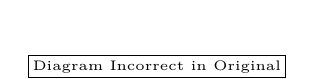
\begin{tikzpicture}
    \tiny
    \setfiguresize{-5.1}{-5.1}{+5.1}{+5.1}
    \begin{scope}[rotate=90]
        \drawevenhexgrid{-5}{-4.5}{11}{10}
        \silentlychangedin{1C}{1C-apj-23-errata}{
            \node at (0,0) [draw,fill=white] {Diagram Incorrect in Original};
        }{
            \begin{scope}[dashed,very thick,->]
                \draw (0,0) --   (0:10);
                \draw (0,0) --  (30:10);
                \draw (0,0) --  (60:10);
                \draw (0,0) --  (90:10);
                \draw (0,0) -- (120:10);
                \draw (0,0) -- (150:10);
                \draw (0,0) -- (180:10);
                \draw (0,0) -- (210:10);
                \draw (0,0) -- (240:10);
                \draw (0,0) -- (270:10);
                \draw (0,0) -- (300:10);
                \draw (0,0) -- (330:10);
            \end{scope}
            \miniathex{+2.0}{+0.0}{\draw node [rotate=90, anchor=south] {\arcline{180} line};}
            \miniathex{-2.0}{-0.0}{\draw node [rotate=90, anchor=south] {\arcline{0} line};}
            \miniathex{+4.0}{+1.0}{\draw node {\minitable{c}{Left\\\arc{180}}};}
            \miniathex{+3.0}{+2.5}{\draw node {\minitable{c}{Left\\\arc{150}}};}
            \miniathex{+1.0}{+3.5}{\draw node {\minitable{c}{Left\\\arc{120}}};}
            \miniathex{-1.0}{+3.5}{\draw node {\minitable{c}{Left\\\arc{90}}};}
            \miniathex{-3.0}{+2.5}{\draw node {\minitable{c}{Left\\\arc{60}}};}
            \miniathex{-4.0}{+1.0}{\draw node {\minitable{c}{Left\\\arc{30}}};}
            \miniathex{-4.0}{-1.0}{\draw node {\minitable{c}{Right\\\arc{30}}};}
            \miniathex{-3.0}{-2.5}{\draw node {\minitable{c}{Right\\\arc{60}}};}
            \miniathex{-1.0}{-3.5}{\draw node {\minitable{c}{Right\\\arc{90}}};}
            \miniathex{+1.0}{-3.5}{\draw node {\minitable{c}{Right\\\arc{120}}};}
            \miniathex{+3.0}{-2.5}{\draw node {\minitable{c}{Right\\\arc{150}}};}
            \miniathex{+4.0}{-1.0}{\draw node {\minitable{c}{Right\\\arc{180}}};}
            \ifaids
                \drawaircraftcounter[90]{+0.00}{+0.00}{60}{F-105}{}{}
            \else
                \drawaircraftcounter[90]{+0.00}{+0.00}{0}{F-105}{A}{2}
                \drawaircraftcounter[90]{+1.00}{-0.50}{210}{MiG-21}{B}{2}
                \drawaircraftcounter[90]{-3.00}{-0.00}{0}{F-105}{C}{2}
            \fi
        }
    \end{scope}
\end{tikzpicture}
\end{fitwidth}
\ifaids\else
\par\bigskip
\begin{minipage}{0.8\linewidth}
A2 is the reference aircraft.

B2 is in the right \arc{150} arc.

C2 is on the \arcline{0} line.

\end{minipage}
\fi
\end{minipage}
\hfil
\begin{minipage}[t]{0.33\linewidth}
\begin{fitwidth}{\linewidth}
\begin{tikzpicture}
    \tiny
    \setfiguresize{-5.1}{-5.1}{+5.1}{+5.1}
    \begin{scope}[rotate=90]
        \drawoddhexgrid{-5}{-4.0}{11}{10}
        \silentlydeletedin{2B}{2B-angle-off-on-hex-side}{
            \begin{scope}[dashed,very thick,->]
                \miniathex{+0.333}{+0.000}{\draw (0,0) -- (300:10);}
                \miniathex{+1.000}{+0.000}{\draw (0,0) -- (330:10);}
                \draw (0,0) --  (0:10);
                \miniathex{+1.000}{+0.000}{\draw (0,0) --  (30:10);}
                \miniathex{+0.333}{+0.000}{\draw (0,0) --  (60:10);}
                \draw (0,0) -- (90:10);
                \miniathex{-0.333}{+0.000}{\draw (0,0) -- (120:10);}
                \miniathex{-1.000}{+0.000}{\draw (0,0) -- (150:10);}
                \draw (0,0) -- (180:10);
                \miniathex{-1.000}{+0.000}{\draw (0,0) -- (210:10);}
                \miniathex{-0.333}{+0.000}{\draw (0,0) -- (240:10);}
                \draw (0,0) -- (270:10);
            \end{scope}
        }
        \silentlyaddedin{2B}{2B-angle-off-on-hex-side}{
            \begin{scope}[dashed,very thick,->]
                \draw (0,0) --   (0:10);
                \draw (0,0) --  (30:10);
                \draw (0,0) --  (60:10);
                \draw (0,0) --  (90:10);
                \draw (0,0) -- (120:10);
                \draw (0,0) -- (150:10);
                \draw (0,0) -- (180:10);
                \draw (0,0) -- (210:10);
                \draw (0,0) -- (240:10);
                \draw (0,0) -- (270:10);
                \draw (0,0) -- (300:10);
                \draw (0,0) -- (330:10);
            \end{scope}        
        }
        \miniathex{+2.0}{+0.0}{\draw node [rotate=90, anchor=south] {\arcline{180} line};}
        \miniathex{-2.0}{-0.0}{\draw node [rotate=90, anchor=south] {\arcline{0} line};}
        \miniathex{+4.0}{+1.0}{\draw node {\minitable{c}{Left\\\arc{180}}};}
        \miniathex{+3.0}{+2.5}{\draw node {\minitable{c}{Left\\\arc{150}}};}
        \miniathex{+1.0}{+3.5}{\draw node {\minitable{c}{Left\\\arc{120}}};}
        \miniathex{-1.0}{+3.5}{\draw node {\minitable{c}{Left\\\arc{90}}};}
        \miniathex{-3.0}{+2.5}{\draw node {\minitable{c}{Left\\\arc{60}}};}
        \miniathex{-4.0}{+1.0}{\draw node {\minitable{c}{Left\\\arc{30}}};}
        \miniathex{-4.0}{-1.0}{\draw node {\minitable{c}{Right\\\arc{30}}};}
        \miniathex{-3.0}{-2.5}{\draw node {\minitable{c}{Right\\\arc{60}}};}
        \miniathex{-1.0}{-3.5}{\draw node {\minitable{c}{Right\\\arc{90}}};}
        \miniathex{+1.0}{-3.5}{\draw node {\minitable{c}{Right\\\arc{120}}};}
        \miniathex{+3.0}{-2.5}{\draw node {\minitable{c}{Right\\\arc{150}}};}
        \miniathex{+4.0}{-1.0}{\draw node {\minitable{c}{Right\\\arc{180}}};}
        \ifaids
            \drawaircraftcounter[90]{+0.0}{+0.00}{0}{MiG-21}{}{}
        \else
            \drawaircraftcounter[90]{+0.00}{+0.00}{0}{MiG-21}{A}{3}
            \drawaircraftcounter[90]{+0.00}{+1.50}{300}{F-4}{B}{3}
            \drawaircraftcounter[90]{-1.00}{+0.00}{30}{F-4}{C}{3}
        \fi
    \end{scope}
\end{tikzpicture}
\end{fitwidth}

\notein{2B}{New angle-off figure for 2B-angle-off-on-hex-side.}

\ifaids\else

\par\bigskip

\begin{minipage}{0.8\linewidth}
A3 is the reference aircraft.

B3 is in the left \arc{90} arc.

C3 is in the right \arc{30} arc (if it was facing A it would be on the \arcline{0} line).

\end{minipage}

\fi
\end{minipage}

\figurecaption{figure:angle-off}{Horizontal arcs.}

\end{twocolumnfigure}
}




%!TEX root = ../rules-working.tex
%LTeX: enabled=false

\begin{twocolumntablefloat}

\begin{twocolumntable}

\tablecaption{table:angle-off-borderlines}{Horizontal Arc Borderline Summary.}
\small
\begin{tabularx}{0.7\linewidth}{lLl}
\toprule
Context&First&Second\\
\midrule
Sensors&Included in the field.&---\\
Jammers&Included in the field.&---\\
Laser Designators&Included in the field.&---\\
Gun and Rocket Attacks&Move the faster element forward.&Use the narrower arc.\\
Blind and Restricted Arcs&Move the faster element forward.&Use the rearward arc.\\
Superior Position&Move the faster element forward.&Use the rearward arc.\\
Missile Launch Envelopes&Move the faster element forward.&Use the wider arc.\\
IRM Launch Target Aspect&Move the faster element forward.&Use the wider arc.\\
Missile Attacks&Move the faster element forward.&Use the wider arc.\\
\bottomrule
\end{tabularx}


\end{twocolumntable}

\vspace{\floatsep}

\begin{twocolumntable}

\tablecaption{table:angle-off-adjacent}{Wider, Narrower, and Rearward Horizontal Arcs.}

\small
\begin{tabularx}{0.7\linewidth}{CCCC}
\toprule
Borderline&Narrower Arc&Wider Arc&Rearward Arc\\
\midrule
\arcline{0}                                &\phantom{0}\arc{30}&\phantom{0}\arc{30}&\phantom{0}\arc{30}\\
\phantom{0}\arc{30} and \arc{60}\phantom{0}&\phantom{0}\arc{30}&\phantom{0}\arc{60}&\phantom{0}\arc{30}\\
\phantom{0}\arc{60} and \arc{90}\phantom{0}&\phantom{0}\arc{60}&\phantom{0}\arc{90}&\phantom{0}\arc{60}\\
\phantom{0}\arc{90} and \arc{120}\phantom{}&\phantom{0}\arc{90}&\phantom{}\arc{120}&\phantom{0}\arc{90}\\
\phantom{}\arc{120} and \arc{150}\phantom{}&\phantom{}\arc{150}&\phantom{}\arc{120}&\phantom{}\arc{120}\\
\phantom{}\arc{150} and \arc{180}\phantom{}&\phantom{}\arc{180}&\phantom{}\arc{150}&\phantom{}\arc{150}\\
\arcline{180}                              &\phantom{}\arc{180}&\phantom{}\arc{180}&\phantom{}\arc{180}\\
\bottomrule
\end{tabularx}

\end{twocolumntable}


\end{twocolumntablefloat}


\paragraph{Angle-Off.} 

The relative horizontal position of the distant element with respect to the reference element is quantified by the horizontal angle between two imaginary lines, one extending behind the tail of the reference element and the other between the reference element and the distant element. This is known as the \emph{angle off the tail} or simply the \emph{angle-off}. 

If the distant element is directly behind the reference element, the angle-off is \arc{0}, if it is directly on the beam, the angle-off is \arc{90}, and if is is directly in front, the angle-off is \arc{180}.

\paragraph{Angle-Off Arcs.} 

Angle-off is grouped into \emph{arcs} covering \arc{30} to the left or right of the target. Figure~\ref{figure:angle-off} show these arcs. The appropriate figure is used according to whether the reference element is in a hex facing a hex corner, in a hex facing a hex side, or on a hex side.

\paragraph{Borderline Procedure.} 

The distant element will often unambiguously be in an angle-off arc. However, sometimes it will be located on the borderline between two arcs. In these case, use the disambiguation procedure described below and summarized in Tables \ref{table:angle-off-borderlines} and \ref{table:angle-off-adjacent}.

In the context of the field of view of sensors, the field of effect of jammers, and the field of laser designators, if either or both of the adjacent arcs are within the field, the borderline is also considered to be within the field. (In other words, the fields include the borderlines.)

In others contexts, if the distant element is on the border between the two \arc{0} arcs or the two \arc{180} arcs, it is considered to be in the \arc{0} arc or \arc{180} arc. This rules does not specify whether aircraft falls in the left or right arcs, but this is never relevant for the game rules. 

% TODO: How do we disambiguate missile envelopes and IRM launch requirements? Included would work for the latter, but not for the former.

For the other borderlines, the procedure for determining the arc is more complex. Consider the speeds of the reference element and distant element at the start of the game turn:
\begin{itemize}
\item If the reference element is slower, the distant element is in the arc it would move into if it moved forward.
\item If the reference element is faster, the distant element is in the arc it would move into if the reference element moved forward.
\item If neither is faster or if the distant element remains on the borderline after one of the previous two cases (i.e., it is facing directly towards or away from the reference element), the resolution again depends on the context:
\begin{itemize}
\item For gun and rocket attacks (rule~\ref{rule:air-to-air-gun-combat}), the distant element (attacking aircraft) is considered to be in the narrower arc.
\item For missile attacks (rule~\ref{rule:missile-attacks}), the distant element (attacking missile) is considered to be in the wider arc.
\item For determining blind and restricted arcs (rule \ref{rule:sighting-aircraft-and-missiles}), the distant element (element being sighted) is considered to be in the rearward arc.
\item For determining advantage purposes (rule~\ref{rule:initiative}), the distant element (element potentially disadvantaged) is considered to be in the rearward arc.
\end{itemize}
\end{itemize}

The narrower arc is the arc further from the \arc{120} arc. The wider arc is the arc closer to the \arc{120} arc. The rearward arc is the arc closer to the \arc{30} arc.

Ground elements are always considered to be slower than any aircraft.

\paragraph{Same-Location Procedure}
If the reference and distant element are at the same map location (i.e., the same hex or hex side), the angle-off arc is the same as it would be if the distant element (i.e., the non-reference element) were moved backwards one hex.

Moving the distant element backwards would always leave it on a borderline facing the reference element and so  requires the use of the disambiguation procedure for borderlines described above.

\paragraph{Angle-Off Lines.} The imaginary lines extending behind and ahead of the reference element are the \arc{0} and \arc{180} lines, respectively. Although not formally arcs, these lines are at times treated as such. To count as being on one of these lines, the distant element must be on the borderline and facing directly along it towards the reference element. If they are on the line but not facing directly along it towards the target, they are considered in either the \arc{30} or \arc{180} arc but not on the \arc{0} or \arc{180} lines.

\paragraph{Angle-Off Examples.}

Consider Figure~\ref{figure:angle-off}, in which the aircraft A1, A2, and A3 are the reference elements and aircraft B1, B2,  B3, C1, C2, and C3 are distant elements. 

Aircraft C2 is unambiguously on the \arc{0} line, and C1 is unambiguously in the right \arc{90} arc, but the other attackers are on borderlines between two arcs. Aircraft C3 cannot be on the \arc{0} line as it is not facing the target, but it is in the \arc{30} arc.

\begin{itemize}

\item
In the context of the field of view of sensors or field of effect of jammers, distant elements on borderlines are considered to be in within the field if either or both of the adjacent arcs are within the field. B1 would be within the field only if either the right \arc{60} arc, the right \arc{90} arc, or both were within the field. B2 would be within the field only if either the right \arc{150} arc, the right \arc{180} arc, or both were within the field. B3 would be within the field only if either the left \arc{90} arc, the left \arc{120} arc, or both were within the field.

\item In other contexts, we need to consider the relative speeds of the reference and distant elements:

\begin{itemize}
\item
If the reference elements were slower than the distant elements, then B2 and B3 would be considered to be in the arcs into which they move if they moved forward: B2 would be in the right \arc{150} arc and B3 would be in the left \arc{120} arc.

\item
If the reference elements were faster than the distant elements, then B2 and B3 would be considered to be in the arcs into which they move if the reference element moved forward: B2 would be in the right \arc{150} arc and B3 would be in the left \arc{90} arc.

\item
If the reference element and the distant aircraft had the same speeds, then the context would determine whether B2 and B3 are considered to be in the narrower, wider, or rearward arc. The same procedure would be used for B1 regardless of the relative speeds, since B1 is facing along a borderline.

\begin{itemize}

\item For gun and rocket attacks, the distant elements are in the narrower arc, so B1 would be in the right \arc{90} arc, B2 in the right \arc{180} arc, and B3 in right \arc{90} arc.

\item For missile attacks (for which the distant elements would be missiles), the distant elements are in the wider arc, so B1 would be in the right \arc{120} arc, B2 in the right \arc{150} arc, and B3 in right \arc{120} arc.

\item For visual sighting and advantage, the distant elements are in the rearward arc, so B1 would be in the right \arc{90} arc, B2 in the right \arc{150} arc, and B3 in right \arc{120} arc.

\end{itemize}

\end{itemize}

\end{itemize}


\paragraph{Ranges of Angle-Off Arcs.}
\label{rule:ranges-of-angle-off-arcs}
Ranges of angle-off arcs are used for restricted or blind regions for sighting, sensor fields of view, and determining advantage. If a range is given as an arc followed by a plus sign, it consists of those arcs and all more forward arcs. If a range is given as an arc followed by a minus sign, it consists of those arcs and all more rearward arcs. Ranges specified in this way consist of both the left and right arcs.

For example, a blind arc given as $\arcrange{60}{-}$ consists the \arc{30} and \arc{60} arcs and a radar search field given as $\arcrange{150}{+}$ consists of the \arc{150} and \arc{180} arcs. 

\paragraph{Lower Angle-Off Arcs.}
\label{rule:lower-angle-off-arcs}
Restricted or blind regions for sighting are sometimes given as \arc{30}L, \arc{60}L, or \arc{180}L. These refer to the \arcrange{30}{-}, \arcrange{60}{-}, or \arcrange{180}{+} arc ranges, but only apply to distant elements at lower altitude.

For example, a restricted arc given as \arc{180}{L} refers to the \arc{180} arcs but only for distant elements at lower altitude. This might apply to an aircraft in which the view from the cockpit forward and downwards is obscured by the nose.

\section{Vertical Limits}
\label{rule:vertical-limits}

}

\section{Aircraft Collisions}
\label{rule:aircraft-collisions}

\CX{
Collisions are possible during the Flight Phase whenever an aircraft executes a head-on gun attack at range zero\addedin{1B}{1B-apj-36-errata}{ and the aircraft are at the same altitude}. Collisions are also possible at the end of \changedin{1B}{1B-apj-36-errata}{a game-turn}{the flight phase} in the following situations:
}{
\paragraph{Potential Collisions.}
Collisions are possible in the following situations:
}

\begin{itemize}
    \IAX{If an aircraft carries out a head-on gun attack at range 0 (see rule~\ref{rule:air-to-air-gun-combat}) on a target at the same altitude.}
    \item \CX{
    If an aircraft is stacked at the same altitude level with any enemy aircraft, and/or
    }{ 
    If an aircraft is stacked at the same altitude as an enemy aircraft after all aircraft have moved. However, aircraft in a tailing chain (see rule~\ref{rule:tailing-enemy-aircraft}) will not collide with each other.
    }
    \item \CX{
    If an aircraft is stacked \addedin{2B}{2B-stacking}{at the same altitude }with two or more friendly aircraft and not in Close Formation.
    }{
    If more than two friendly aircraft are stacked at the same altitude after all aircraft have moved and they are not in a close formation (see rule~\ref{rule:close-formations}).
    }
    \itemaddedin{2B}{2B-stacking}{If more than four friendly aircraft are stacked at the same altitude after all aircraft have moved, even if they are in a close formation.}
\end{itemize}

\CX{
\paragraph{Collision Resolution.} 
\addedin{2B}{2B-collisions}{Potential collisions resulting from head-on gun attacks are resolved immediately after the attack. Other potential collisions are resolved at the end of the flight phase.} For each potential collision, the player who last moved into the position must roll the die. On a roll of 1, his aircraft collides with one of the others. Determine which aircraft it collides with randomly. Both aircraft immediately roll on the 10 column of the Damage table to determine their damage.

\paragraph{Collision Exceptions:} There are \changedin{1B}{1B-apj-36-errata}{two}{three} exceptions to the Potential Collision rule.

\begin{itemize}
    \item An aircraft tailing another will not collide with that aircraft.
    \item An aircraft which is flying in close formation will not collide with other friendly aircraft in that formation.
    \itemaddedin{1B}{1B-apj-36-errata}{An aircraft that has already rolled for a collision for a head-on gun attack does not roll again for a collision \addedin{2B}{2B-collisions}{at the same position }again at the end of the flight phase.}
\end{itemize}

\notein{1B}{AWF: There is a clarification of the collision exceptions in the APJ 23 errata, but it seems to restate the original exceptions. I have not included it.}

}{
\paragraph{Collision Resolution Procedure.} 
If an aircraft carries out a head-on gun attack at range 0 and the same altitude, it immediately checks for a collision. The other cases are resolved at the end of the flight phase. Of the aircraft that could collide and which have not already checked for a collision at the same position (because of a head-on gun attack), the one that moved last checks for a collision. To check for a collision, roll the die. On a roll of 1, the aircraft collides with one of the others. Determine the other aircraft randomly. Both aircraft suffer damage from a weapon with an attack rating of 10 (see rule~\ref{rule:aircraft-damage-resolution}).
}


\section{Aircraft Data Cards}

This chapter discusses the Aircraft Data Cards (ADCs) and the information presented on them. Each aircraft used in play has its flight and combat capabilities fully defined in game terms in its ADC. A sample ADC is shown on the following pages.  It is divided into two major panels: The Flight Characteristics panel and the Combat Characteristics panel.

\subsection{Flight Characteristics Panel}

\changedin{1C}{AMW}{

\begin{FIGURE*}[!ht]
\includegraphics[width=0.7\linewidth]{figures/figure-adc-flight-side.pdf}
\includegraphics[width=0.7\linewidth]{figures/figure-adc-combat-side.pdf}
\end{FIGURE*}

}{
\begin{FIGURE*}[!ht]

\newcommand{\drawleftlabel}[3]{
    \draw [thick,->] (-8.5,#3-0.3*8.5-0.3*#2) [anchor=east, inner sep=1mm] node {\normalsize #1} -- (#2,#3);
}
\newcommand{\drawrightlabel}[3]{
    \draw [thick,->] (+8.5,#3+0.3*8.5-0.3*#2) [anchor=west, inner sep=1mm] node {\normalsize #1} -- (#2,#3);
}

\begin{tikzfigure}{\linewidth}

% Fix the width.
\draw [color=white] (-10,0) -- (+10,0);

\changedin{2A}{AMW}{
\draw (+0.0,-0.05) node 
    {\includegraphics[width=14cm]{figures/figure-adc-first-edition.png}};
}{
\draw (+0.0,+0) node 
    {\includegraphics[width=14cm]{figures/figure-adc-second-edition.png}};
}
%\draw[step=1cm,color=black!20] (-10,-10) grid (10,12);

\drawleftlabel{1}{-6.7}{+9.0}
\drawleftlabel{2}{-2.3}{+6.9}
\drawleftlabel{3}{-2.4}{+4.7}
\drawrightlabel{4}{+6.7}{+8.0}
\drawleftlabel{5}{-6.7}{+7.40}
\drawleftlabel{6}{-6.7}{+4.2}
\drawrightlabel{7}{+6.7}{+7.0}
\drawrightlabel{8}{+6.7}{+4.2}
\drawleftlabel{9}{-6.7}{-0.8}
\drawleftlabel{10}{-2.5}{-0.8}
\drawleftlabel{11}{-6.7}{-3.05}
\drawleftlabel{12}{-6.7}{-5.35}
\drawleftlabel{13}{-2.5}{-3.05}
\drawrightlabel{14}{+6.7}{-0.8}
\drawrightlabel{15}{+6.7}{-3.2}
\drawrightlabel{16}{+3.9}{-3.6}
\drawrightlabel{17}{+6.7}{-4.2}
\drawleftlabel{18}{-6.7}{-6.1}
\drawrightlabel{19}{+6.7}{-8.9}

\end{tikzfigure}

\CAPTION{figure:adc}{An aircraft data card (ADC).}

\end{FIGURE*}
}
    
The Flight Characteristics panel is the top half of the ADC and it contains information which defines the flying capabilities of the aircraft. This panel is divided into the following sections:

\begin{enumerate}

    \item \itemparagraph{Aircraft Type.} The upper right corner contains the name most commonly used to identify that type of aircraft. It also shows the number of crew positions on the aircraft.

    \item \itemparagraph{Three-View.} The 3-view drawing is included to familiarize the player with the appearance of the aircraft. The top view will be similar to that used on a corresponding game counter.

    \item \itemparagraph{Basic Data.} The center of the panel contains the basic information chart which includes:
    \begin{itemize}
        \item Cruise Speed: This is the cruise speed of the aircraft shown in Flight Points (FPs).
        \item Climb Speed: The optimum climb speed of the aircraft shown in FPs.
        \item Visibility: This is a visibility rating number referenced for sighting attempts against the aircraft.
        \item Size: This is the size modifier used as an enemy “to hit" die roll modifier in combat.
        \item Vulnerability: This is the vulnerability modifier used as a damage die roll modifier.
        \item Restricted Arc: This defines the aircraft's angle-off arc into which it can sight enemies only with difficulty.
        \item Blind Arc: This defines the aircraft's angle-off arc into which it cannot sight enemies.
        \item Internal Fuel: This is the maximum quantity of internal fuel, in terms of points, that can be carried by the aircraft.
        \item Ata Refuel: The yes or no indicates whether or not the aircraft can refuel from aerial tankers in flight.
        \item Ejection Seat: This lists the type of egress system carried by the aircraft; either none, early, standard or advanced ejection seats.
    \end{itemize}

    \item \itemparagraph{Maneuver Costs.} The Maneuver Costs Chart shows the cost, in terms of Flight Points and Decel Points, to perform lag rolls, displacement rolls, and vertical rolls. The cost is paid each time one of these maneuvers is performed.

    \item \itemparagraph{Power Chart.} The Power Chart indicates the maximum number of Accel Points available to the aircraft in a single game turn when a specific power setting is selected for the aircraft's engines. Three columns appear, one for each possible configuration of the aircraft. \changedin{2A}{2A:idle,2A:spbr,2A:fp-to-dp}{Also shown is the speed loss (in FPs) for selecting idle power and/or speedbrakes, and the fuel points used at each power setting.}{\par Also shown is the deceleration in DPs for selecting idle power and/or speedbrakes. (In earlier ADCs, these rows are labeled “Idle FP” and “Spbr.\ FP”, and the values should be doubled to obtain the corresponding number of DPs.) \par The last column shows the fuel points used at each power setting.}

    Note: The dots to the right of the Power Chart heading indicate the number of engines the aircraft has.

    \item \itemparagraph{Minimum-Maximum Velocity Chart.} The Minimum-Maximum Velocity Chart shows the minimum and maximum allowed speeds of the aircraft (in terms of Flight Points) in each altitude band by configuration. The Dive Speed column indicates the maximum speed (in Flight Points) allowed regardless of aircraft's configuration after a turn of Diving flight. The maximum ceiling, in altitude levels, that can be climbed to in each configuration is also indicated here.

    \item \itemparagraph{Turn Drag Chart.} The Turn Drag Chart shows the decel points received by an aircraft each game turn when using one of the listed turn rates. Three columns appear, one for each possible configuration. Appropriate notes are shown for the Turn Drag Chart if necessary.

    \item \itemparagraph{Climb Capability Chart.} The Climb Capability Chart (CCC) shows the maximum number of altitude levels an aircraft can gain in a single game turn at the Sustained Climb decel rate while in afterburner power or any other power in each altitude band for each possible configuration.

\end{enumerate}

Note: The game terms “configuration”, “accel point”, “decel point”, “flight point", and “angle-off arcs” may seem foreign to you at this moment. Do not be alarmed, each term will be clearly explained and its game function defined in upcoming chapters. Please read on.

\subsection{Combat Capabilities Panel}

The Combat Capabilities Panel is the lower half of the ADC and contains information about the combat abilities of the aircraft.  The panel is divided into the following sections.

\begin{enumerate}[resume]

    \item \itemparagraph{Radar Data.} The Radar section indicates the characteristics of the aircraft's radar system. The search and tracking ranges are described in terms of hexes of distance. The functions of radar arcs, ECCM numbers and lock-on numbers are described in the radar rules.

    \item \itemparagraph{ECM Data.} The ECM section shows the types of electronic counter-measures gear, if any, the aircraft carries. ECM gear is identified by type (i.e., RWR = radar warning receiver) and quality. A dash indicates no gear of that type is present. A letter indicates gear is present and also indicates the relative quality of the equipment, (i.e., A = least capable, B and C = improved gear, and D = best). The number after the letter is its capability rating as explained in the ECM rules.

    \item \itemparagraph{Internal Gun Data.} The Internal Gun section shows the characteristics of the aircraft's internal guns if any. The data is fully explained in the gun combat rules (Rule 9).

    \item \itemparagraph{Bomb System.} The Bomb System section lists the kind of bombsight carried and the attack die roll modifier it provides when the aircraft does air to ground attacks.

    \item \itemparagraph{Technology Listing.} The Technology section lists the kinds of technology, if any, available to the aircraft. The effects on play of having a listed technology is defined in the appropriate rules sections.

    \item \itemparagraph{Weapons Stations Diagram.} The Weapon Stations Diagram identifies (by number) the aircraft's weapons pylons or internal bays. These weapons stations are where bombs, missiles, and other stores are attached to the aircraft. At the start of play, each aircraft should have its load of weapons and stores recorded on paper to facilitate keeping track of changes in the load as weapons are expended.

    \item \itemparagraph{Configuration Points Limits.} This section indicates what configuration an aircraft will be in when carrying a given amount of weapons and/or other loads. Every weapon, fuel tank, or store that can be carried is given a point value called its “load point rating” (see the associated weapons tables). These load points represent the weight and drag penalty that the item imposes on an aircraft when carried.

    The sum of the load an aircraft is carrying at any instant, in load points (rounded down), is compared to the limits given for the three possible configurations (CL = clean, 1/2 = half dirty, DT = Dirty). Where the sum falls within those limits defines the current configuration of the aircraft. See advanced rule 4.3.

    Internal Weapons Bays Note:  All weapons or stores carried in an aircraft's internal weapons bay count for only half the normal load value since no drag is imposed on the airplane.

    Basic Rules Note:  Use Only the CL Conf. Data. The term “configuration” refers to the relative load an aircraft is carrying. At the basic level of play aircraft are always considered to be “CL” or “Clean” configured. Players need only refer to the information under the "CL" sections of the ADC. They need not worry about changes in configuration, nor about load points or about information under the “1/2” or “DT” columns.

    \item \itemparagraph{Load Limit.} The load limit shown for the aircraft, in pounds, is the maximum weight of weapons and stores it can carry. All weapons and other stores listed in the game have a weight shown for them in the weapons charts. The aircraft's load may never exceed this amount even if the sum of all its station limits might be higher.

    \item \itemparagraph{Station Limits.} Each weapons station is limited in the amount of weight it can carry. This section lists each station's weight limit, and the types of ordnance and equipment which can be placed on the station. The types of loads that may be placed on each station are indicated in letter codes (i.e., BB = Ballistic Bombs, RP = Rocket Pods, etc.). The listed codes correspond to the codes given in the weapons tables.

    \item \itemparagraph{Notes and Variants.} The Notes and Variants section may contain additional comments about the aircraft and its capabilities. When a significant variant aircraft type is available, its differences from the basic ADC are shown.

    \item \itemparagraph{Victory Points.} The number of scenario victory points awarded to the enemy for achieving a level of damage against that aircraft is shown here. The four numbers are for K, C, H, and L damage levels respectively (Killed, Crippled, Heavy, and Light).

\end{enumerate}

\advancedrules

\subsection{Aircraft Configuration}

An aircraft carrying a load of bombs or other stores under its wings is less streamlined, and significantly heavier than a similar aircraft which is not. As a consequence, its performance will suffer in proportion to the load it carries. This is reflected through the concept of aircraft configuration.

\paragraph{Configuration.} Aircraft can be flown in one of three possible game configurations: Clean (CL), Half Dirty (1/2), and Dirty (DT). The actual configuration is determined by the amount of load points carried on the aircraft's weapons stations.  Each Aircraft Data Card indicates the point limits which establish Clean, Half, and Dirty. When adding up the load, first total all points then round any fractions \changedin{1B}{1B:apj-23-errata}{off}{down}.

\paragraph{Clean (CL).} An aircraft in clean configuration is unencumbered by external ordnance or equipment (it may carry some external equipment, but not enough to produce appreciable drag). Generally, the data cards are rated so that fighters can carry a normal load of missiles without penalty.

\paragraph{Half (1/2).} An aircraft in half configuration is midway between the lack of drag of Clean and the full drag of Dirty. Usually, adding a drop tank, and/or ECM pods or a small load of bombs is enough to cause a fighter to be half-loaded.

\paragraph{Dirty (DT).} An aircraft in Dirty configuration experiences substantial drag from external add-ons. Carrying a large load of ordnance and/or drop tanks will suffice to cause a fighter to be considered Dirty. You will note, that DT configured aircraft have lower speeds, less power, and suffer more Decel penalties while maneuvering than lesser configured aircraft.

\paragraph{Changes in Configuration.} An aircraft's configuration is never fixed, and will change during play as weapons are expended in attacks or jettisoned as the situation warrants. Changes in configuration take effect the instant enough load is disposed of to allow the point total to fall within a lesser limit.

Changes in configuration effect several aspects of play and are handled as follows:

\begin{itemize}

    \item Power Available: Configuration changes can only occur after the power setting is selected, so no increase in Accel is available until the following turn.

    \itemaddedin{2B}{AWF}{Cruise Speed. If idle or normal power is selected, the determination of the cruise speed uses the configuration at the start of a game turn.}

    \item When Turning: The turn drag decel points an aircraft receives for turning is that for the configuration which existed when the highest turn rate was used that game turn.

    \item When Climbing: The climb rate allowed is that of the configuration which exists when the aircraft expends its first VFP during the game turn.

\end{itemize}

\addedin{1B}{1B:apj-23-errata}{\paragraph{Over-Loading Stations.} An aircraft may overload any of its weapon stations in terms of weight by up to 20\%. However, its maximum turn capability is reduced by one (i.e., from BT to HT) until all overloaded stations are back within limits. Though stations may be overloaded, the aircraft's total load limit may never be exceeded.}

\addedin{1B}{1B:apj-23-errata}{\paragraph{Symmetric Loading Requirements.} When picking loads for aircraft, the initial weight carried on one wing must be within 20\% of that carried on the other wind unless the total weight on each wing is 10\% or less of the aircraft's load limit.}

Configuration Example: An aircraft with the following configuration limits: CL = 0-8, 1/2 = 9-14, and DT = 15+; that is loaded with two Triple Racks (TRs) and six Mk.82 500lb HE bombs, is carrying 11 load points and would be 1/2 configured. The TRs are worth one load point each and the bombs are 1.5 points each. If a 1200L fuel tank were added (4 load points), the aircraft would be considered DT configured (15 points total).

\subsection{Jettisoning Weapons and Stores}

Aircraft may voluntarily jettison weapons and/or stores to change configuration, or may be required to jettison them due to combat damage. If voluntary, the player may selectively choose which weapons/stores, and how many, are jettisoned. If a required action due to damage, enough weapons and/or stores, player's choice, must be jettisoned to allow the aircraft to become CL configured.

\paragraph{Jettison Procedure.} Weapons and/or stores may be jettisoned by simply announcing the act during an aircraft's move. The configuration change takes effect immediately after the aircraft's next expenditure of an FP in movement.

%!TEX root = ./rules-working.tex
%LTeX: enabled=false

\rulechapter{Aircraft Flight}

\silentlyaddedin{1B}{1B-tables}{
    %!TEX root = ../rules-working.tex
%LTeX: enabled=false

\begin{twocolumntablefloat}
\begin{twocolumntable}

\newcommand{\heading}[1]{\medskip\par\textbf{\MakeUppercase{#1}}\par\smallskip}
\newcommand{\subheading}[1]{\smallskip\par\textbf{#1}\par\smallskip}

\tablecaption{table:aircraft-flight-rules-summary}{Aircraft Flight Rules Summary}
\footnotesize
\begin{tabularx}{\linewidth}{P}
\toprule
\begin{multicols}{2}

\heading{Accel/Decel}
\begin{enumerate}[nosep]
    \item Each 2.0 accel accumulated = \plus{0.5} speed normally.
    \item Each 1.5 accel = \plus{0.5} speed for Rapid Accel aircraft.
    \item If speed ≥ Mach 1, each 3.0 accel = \plus{0.5} speed for normal aircraft and each 2.0 = \plus{0.5} for Rapid Accel aircraft.
    \item Each 2.0 Decel accumulated = \minus{0.5} speed always.
\end{enumerate}

\heading{Level Flight}
\begin{enumerate}[nosep]
    \item All FPs are HFPs. An aircraft may descend one altitude level freely at any point in its move.
\end{enumerate}

\heading{Turning Flight}
\begin{enumerate}[nosep]
    \item Turn Drag decel based on highest turn rate used in game turn, incur it only once per game turn even if aircraft faced more often than once.
    \item \changedin{2A}{2A-sustained}{Extra facings in a game turn constitute sustained turns. 1.0 decel is incurred for each dacing change after the first.}{The second and subsequent facing change in a game turn constitute sustained turns. 1.0 DP are incurred for each 30 degrees of facing change in sustained turns (0.5 DP for LBR and 1.5 DP for HBR aircraft).}
    \item TT, HT, BT, ET turns require start speed of 0.5, 1.0, 1.5, and 2.0 > minimum respectively to perform.
    \item Low Roll Rate aircraft take 1 FP of flight to enter a left or right bank before turning and 2 FPs of flight to reverse bank.
    \item High Roll Rate aircraft may instantly switch from one angle of bank to another; others require 1 FP of flight to reverse.
    \item No attacks of weapon launches allowed during or after an ET turn until a Recovery Period passes.
    \item[--] A recovery period = half of the aircraft's flight (round up) while not ET turning and not doing rolls or prep-moving for them.
\end{enumerate}

\deletedin{2A}{2A-snap}{
\heading{Snap Turning}
\begin{enumerate}[nosep]
    \item Aircraft must be capable of BT turn rate.
    \item One allowed per game-turn; costs one HFP; allows immediate facing change of 30 degrees or of 60 degrees if turn chart = 60 or 90 without moving forward.
    \item One HFP prep required is wings not level or if speed ≥ to High Transonic. If both cases apply, two preps required.
    \item Incur Decel as for BT turn unless aircraft used ET rate.
    \item Unless ET follows a snap turn; the snap counts as a BT turn for purposes of combat and weapon launch modifiers until a recovery period passes.
    \item Risky Snap turns may be tried if aircraft is capable of HT turn but roll for a departure on facing (1 to 4).    
\end{enumerate}
}

\heading{FP Expenditure Restrictions}
\begin{enumerate}[nosep]
    \item If going from level to climbing or diving flight; the first FP expended must be an HFP.
    \item If going from dive to climb or climb to dive; FPs = to half the aircraft's speed (round down) must be expended as HFPs before using VFPs. High Pitch Rate aircraft need only expend FPs = to {\onethird} speed (round down) in this case.
    \item If continuing to climb or dive from previous turn; HFPs and VFPs may be mixed in any order.
\end{enumerate}

\vfill\null\columnbreak

\heading{Speedbrake Usage}
\changedin{2A}{2A-spbr}{
\begin{enumerate}[nosep]
    \item FPs up to amount listed on the ADC may be eliminated.
    \item Eliminated FPs may not be used for any turns or other maneuver/combat/proportional move requirements.
    \item 1.0 decel is incurred for each 0.5 FP eliminated.
\end{enumerate}
}{
\begin{enumerate}[nosep]
    \item DPs up to the maximum listed on the ADC may be incurred.
    \item If the aircraft is supersonic, the maximum is increased by 1 DP.
\end{enumerate}
}

\heading{Climbing Flight}

\subheading{Zoom Climbs}
\begin{enumerate}[nosep]
    \item At least one, but up to {\twothirds} of FPs may be VFPs.
    \item If CCC rate for power setting ≤ 2.0, then each VFP can gain 1 altitude level only.
    \item If CCC rate for power setting > 2, each VFP can gain 1 or 2 altitude levels.
    \itemaddedin{2A}{2A-super-climbs}{If CCC rate for power setting ≥ 6.0, one of the VFPs can gain 1, 2, or 3 altitude levels.}
    \itemdeletedin{2A}{2A-zoom-climbs}{If this is the first turn of climbing flight, 1.0 decel is incurred per level climbed.}
    \itemdeletedin{2A}{2A-zoom-climbs}{If this is the second or subsequent turn of climbing flight, 1.5 decel is incurred per level climbed.}
    \itemaddedin{2A}{2A-zoom-climbs}{1.0 DP per level climbed.}
    \item ET turn rates not allowed in zoom climbs.
\end{enumerate}

\subheading{Sustained Climbs}
\begin{enumerate}[nosep]
    \item Start speed must be at least 1.0 > minimum speed.
    \item If start speed is less than climb speed, then halve CCC value (retain fractions).
    \item If CCC value is < than 1.0, only one VFP may be used in game-turn and it gains only the fractional altitude level.
    \item If CCC value ≥ 1.0 but ≤ 2.0, up to 2/3s of the FPs may be VFPs. The first VFP gains any listed fraction (or 1 if no fractions listed), and the rest gain one altitude level each.
    \item If CCC value is > 2.0, up to 2/3s of the FPs may be VFPs. The first VFP gains 1.0 level \plus{} any fraction and the rest may gain 1.0 or 2.0 altitude levels each.
    \itemaddedin{2A}{2A-super-climbs}{If CCC value ≥ 6.0, one of the VFPs after the first can gain 1, 2, or 3 altitude levels.}
    \item If enough VFPs exist, an aircraft may climb more levels than listed on the CCC. However, the extra levels climbed cause decel as if zoom climbing.
    \item Only EZ turns and Slide maneuvers allowed.
    \item 0.5 decel is incurred for each level up to the CCC limit. Extra levels incur decel as for zoom climbing\addedin{2A}{2A-zoom-climbs}{\ at 1.0 DP per level climbed.}.
\end{enumerate}

\subheading{Vertical Climbs}
\begin{enumerate}[nosep]
    \item Previous game-turn must have involved climbing flight.
    \item Exception; High Pitch Rate aircraft may enter vertical climbs from level flight if speed < 4.0.
    \item On first turn of vertical climb, {\onethird} of FPs must be HFPs. If vertical climb continued, not more than {\onethird} of FPs may be HFPs and up to all may be VFPs.
    \item Each VFP may gain 1.0 or 2.0 altitude levels each.
    \item Each level climbed causes \changedin{2A}{2A-vertical-climbs}{2.0}{1.5} decel points.
    \item No turns or maneuvers except Vertical Rolls allowed.
    \item Diving flight may not follow Vertical climbs.
    \item Exception, High Pitch Rate aircraft may enter Steep Dives or Unloaded Dives the turn after.
    \item Exception, normal aircraft may use a Half-Roll and Dive maneuver to enter Steep Dives after a Vertical Climb.
\end{enumerate}


\end{multicols}
\\
\bottomrule
\end{tabularx}
\end{twocolumntable}
\end{twocolumntablefloat}

\begin{twocolumntablefloat}
\begin{twocolumntable}

\newcommand{\heading}[1]{\medskip\par\textbf{\MakeUppercase{#1}}\par\smallskip}
\newcommand{\subheading}[1]{\smallskip\par\textbf{#1}\par\smallskip}

\tablecaptioncontinued{table:aircraft-flight-rules-summary}{Aircraft Flight Rules Summary}
\footnotesize
\begin{tabularx}{\linewidth}{P}
\toprule
\begin{multicols}{2}

\heading{Diving Flight}

\subheading{Steep Dives}

\begin{enumerate}[nosep]
    \item At least one FP must be and up to 2/3s FPs may be VFPs.
    \item Each VFP may Lose 1.0 or 2.0 altitude levels.
    \itemdeletedin{2A}{2A-steep-dives}{Each level dived gains 0.5 accel on the first turn of Diving.}
    \itemdeletedin{2A}{2A-steep-dives}{If this is the second or subsequent turn of
    continuous Diving, each level dive gains 1.0 accel.}
    \itemaddedin{2A}{2A-steep-dives}{1.0 AP per level.}
\end{enumerate}

\subheading{Unloaded Dives}

\changedin{XX}{XX-unloaded-dives}{
\begin{enumerate}[nosep]
    \item \changedin{2A}{2A-unloaded-dives}{All FPs are HFPs.}{One or two FPs are VFPs. The rest are HFPs.}
    \item \changedin{2A}{2A-unloaded-dives}{At least 1 HFP must be expended with the aircraft “unloaded”. More than 1 and up to all may be expended “unloaded”.}{The first VFP may only be used after half of the HFPs have been expended with the aircraft unloaded. The second VPF may only be used after all of the HFPs have been expended with the aircraft unloaded.}
    \item \changedin{2A}{2A-unloaded-dives}{Each HFP expended while unloaded moves the aircraft forward one hex/hexside and loses it one altitude level.}{The aircraft loses 1 level on each VFP.}
    \item \changedin{2A}{2A-unloaded-dives}{The aircraft gains accel as if Steep Diving.}{The aircraft gains 1.0 AP per level lost.}
    \item The aircraft may not make any attacks, guide weapons or aim while unloaded.
    \item \changedin{2A}{2A-unloaded-dives}{FPs done while unloaded may not be used for turning or prep-moving.}{Unloaded FPs may not be used for turning flight or for preparing or executing any maneuver except a slide.}
    \item All unloaded \changedin{2A}{2A-unloaded-dives}{HFPs}{FPs} done in a single game-turn must be done in one continuous string.
\end{enumerate}
}{
\begin{enumerate}[nosep]
    \item All FPs are HFPs.
    \item At least half of the HFPs (round down) must be expended with the aircraft “unloaded”. All unloaded HFPs must be consecutive.
    \item The aircraft loses on altitude level after half of the HFPs (round down) have expended unloaded. If all of the HFPS are expended unloaded, the aircraft loses another altitude level after the last HFP.
    \item The aircraft gains 1.0 AP per level lost.
    \item The aircraft may not make any attacks, aim, track targets, launch or guide weapons or use radar while unloaded and until it completes a recovery period.
    \item Unloaded FPs may not be used for turning flight or for preparing or executing any maneuver except a slide.
\end{enumerate}
}

\subheading{Vertical Dives}

\begin{enumerate}[nosep]
    \item Previous game turn must have involved diving flight.
    \item Exceptions: a vertical dive may be entered from level flight using a Half Roll and Dive maneuver. If start speed ≤ 4.0, it may also be entered from a zoom or sustained climb by using a Half Roll and Dive maneuver.
    \item On first turn of vertical diving, 1/3 of FPs must be HFPs. If vertical dive continued, no more than 1/3 of FPs may be HFPs and up to all may be VFPs.
    \item Each VFP must lose 2.0 or 3.0 altitude levels.
    \item Each altitude dived gains 1.0 accel.
    \item No turns or maneuvers except vertical rolls allowed.
    \item Climbing flight may never follow vertical dives.
    \item Level flight may follow if A/C's new start speed is 3.0 or less for High Pitch Rate aircraft, or 2.0 or less for others.
    \item[--] If case 8 does not apply, diving flight must follow vertical dive.
    \item When Steep or Unloaded dives follow a vertical dive; at least half an aircraft's FPs (round down) must be expended as VFPs or Unloaded HFPs; except High Pitch Rate aircraft need only expend 1/3 FPs as VFPs or unloaded HFPs.
\end{enumerate}

\heading{Stalled Flight}

\begin{enumerate}[nosep]
    \item Aircraft does not move or change facing.
    \item Altitude lose = start speed (round 0.5 up) + 1.0; increase loss by 1.0 per additional turn of stalled flight.
    \item Aircraft gains accel as it steep diving and by power.
    \item Aircraft may recover to level or diving flight including immediately entering a vertical dive.
\end{enumerate}

\heading{Departed Flight}

\begin{enumerate}[nosep]
    \item Stay in same hex; randomly change facing left or right.
    \item Roll die to find number of facing changes in that direction.
    \item Altitude loss = start speed (round 0.5 up) + 2.0; increase altitude loss by 2.0 per additional turn of departed flight.
    \item Power has no effect, all accel/decel = 0 whole departed.
    \item Recovery is via recovery roll (\minusafter{6} including modifiers).
    \item Upon recovery aircraft must enter diving flight (vertical dives allowed). High Pitch Rate aircraft may recover to level flight.
    \item Upon recovery, start speed reverts to higher of Minimum speed or speed at which departure occurred.
\end{enumerate}

\heading{Aircraft Maneuvers}

\subheading{Slides}

\begin{enumerate}[nosep]
    \item Expend two HFPs to prep for slide. One HFP to execute.
    \item 1 slide allowed if speed ≤ 9.0, two if speed > 9.0 but at least 4 FPs must be expended between execution of first and start of preps for second.
    \item One slide causes no decel; two slides cause 1.0 decel.
\end{enumerate}

\subheading{Lag/Displacement Rolls}

\begin{enumerate}[nosep]
    \item Expend \changedin{2A}{2A-roll-preparatory-fps}{one HFP}{FPs equal to {\onethird} of speed (round down)} to prep for rolls. One HFP to execute.
    \item Shift in direction of roll (see \changedin{1B}{1B-figures}{diagram}{Figures~\ref{figure:displacement-roll-maneuvers} and \ref{figure:lag-roll-maneuvers}}) and optionally face 30 degrees in direction opposite to roll.
    \item A displacement roll from a hexside shifts the aircraft to a hexside as in a slide and not sideways as depicted for the lag roll. Decel for these rolls varies, see ADC.
\end{enumerate}

\subheading{Vertical Rolls}

\begin{enumerate}[nosep]
    \item Aircraft must be in vertical climb or dive and must have just expended a VFP.
    \item Change facing left or right up to 180 degrees.
    \item Decel cost varies; see ADC.
    \item Multiple vertical rolls allowed in a single game turn but each must occur after separate VFP expenditures.
\end{enumerate}

\subheading{Barrel Rolls}

\begin{enumerate}[nosep]
    \item Executed as 2 or more consecutive Lag/Displacement rolls.
    \item If done in level flight, 1 altitude level may be gained or lost upon executing last roll at no additional FP code.
    \itemaddedin{1C}{1C-apj-39-qa}{If done in climbing or diving flight, 1 altitude level may be gained or lost upon executing each roll after the first at no additional FP cost.}
    \item Altitude changes that occur in a diving or climbing B-Roll may be in lieu of, or in conjunction with altitude changes done via VFP expenditure.
    \item Incur 2.0 decel per level gained in climbing Barrel Roll, and gain 0.5 accel per altitude level lost in a Barrel Roll.
\end{enumerate}

\subheading{Half Roll and Dive}

\begin{enumerate}[nosep]
    \item Declare at start of move, perform normal Vertical dive except no vertical rolls allowed until last FP expended and then only if it was a VFP.
    \item Allow vertical dive entry from level flight, ot if speed ≤ 4.0 allows entry from zoom/sustained climbs.
    \item Allows steep dive entry from vertical climbs, with normal turning allowed.
    \item No attacks or weapon launches allowed that turn.
\end{enumerate}

\begin{itemize}[nosep]
    \item For purposes of weapons launch modifiers and gunsights, rolls count as BT turns until recovery period met.
    \item Incur 1.0 extra decel for each roll over one executed in a signle game-turn.
\end{itemize}

\heading{VIFF Maneuvers (VIFF Capable aircraft only)}

\subheading{VIFF Sidestep}

\begin{enumerate}[nosep]
    \item Executed as a slide except no prep-moves required but those imposed by altitude and supersonic speed.
    \item Multiple sidesteps allowed so long as 1 HFP expended in forward flight between execution of each sidestep.
    \item Each costs two HFPs to execute and each causes 2.0 decel.
\end{enumerate}

\subheading{VIFF Assisted Turn}

\begin{enumerate}[nosep]
    \item Reduce listed turn requirements by one (90 is best allowed).
    \item Treat aircraft as High Bleed Rate, incur 2.0 to use.
\end{enumerate}

\subheading{VIFF Vertical Pitch}

\begin{enumerate}[nosep]
    \item Treat as Half Roll and Dive except aircraft may go from vertical climb direct to vertical dive, incur 2.0 decel.
\end{enumerate}

\subheading{VIFF Pop-up}

\begin{enumerate}[nosep]
    \item Allows gain of one Altitude Level from level flight once per turn.
    \item Costs 1 HFP, incurs 2.0 decel, aircraft must be wings level.
\end{enumerate}

\end{multicols}
\\
\bottomrule
\end{tabularx}
\end{twocolumntable}
\end{twocolumntablefloat}

}

An aircraft is flown, in game turns, by moving it horizontally across the game maps and tracking its changes in speed and altitude on an Aircraft Log Sheet.\addedin{1B}{1B-tables}{\ The aircraft flight rules are summarized in Table~\ref{table:aircraft-flight-rules-summary} and detailed in the following chapters.} An aircraft is allowed to move and make changes in altitude by expending Flight Points (FPs). Generally, one flight point moves the aircraft one hex on the map, or up or down one or more levels of altitude. The speed of an aircraft determines how many flight points it has each turn.


\section{The Aircraft Log}
\label{rule:aircraft-log-sheets}

An aircraft log sheet is used to record the starting speed and altitude of an aircraft each turn. Different actions an aircraft may take will affect its speed and altitude from one turn to the next. The different lines on the log provide spaces to record these actions and to calculate resultant changes in speed and altitude. A pad of generic aircraft log sheets is provided with each game. One log should be used for each aircraft in play. A log sheet is divided into 15 columns, enough to record 15 turns of play (about the average length of a game). If you run short you may make copies of the sheets. Where applicable, the various rules sections which follow will provide additional information on using the log sheet.

\paragraph{Set Up Information.} 
When a scenario is set up, each aircraft must be given a start altitude level, and speed. These are noted in lines 1 and 2 of column one of the log sheets. Any scenarios provided in the game will establish these values in their set up instructions. If you create your own scenarios, you will have to decide on these values yourself. Once aircraft and any other required counters are placed on the maps, and the start speeds and altitudes are noted, play may commence.

\paragraph{Using The Log Sheet.} 
As an aircraft is maneuvered, it might change altitude and/or accumulate accel and decel points. The accumulation of accel and/or decel Points may cause changes in the aircraft's speed so spaces are provided on the log to record these points. Spaces are also provided to calculate changes in an aircraft's speed and/or altitude. The final altitude and speed at the end of one game turn becomes the new start speed and altitude for the next game turn.

\section{Flight Points}
\label{rule:flight-points}

The speed of an aircraft is always expressed in terms of Flight Points (FPs), each of which equates to 100 mph of speed. An aircraft with a speed of 5.5 would be traveling at 550 mph. Flight Points are expended to move an aircraft across the game map and/or to change altitude.  An aircraft must expend all whole FPs available to it each game turn. Any unused 0.5 FP remaining can be ignored. An FP may be either a horizontal FP or a vertical FP depending on how it is used.

\paragraph{Horizontal Flight Points.} 
FPs expended to move horizontally across the map are called Horizontal Flight Points (HFPs). One HFP is spent to move an aircraft forward one hex or hexside. It may only fly onto a hexside if it faces parallel to that hexside (see 3.1).

\paragraph{Vertical Flight Points.} 
FPs expended to gain or lose altitude levels are called Vertical Flight Points (VFPs). The amount of altitude levels gained or lost with the expenditure of each VFP varies with the exact type of climb or dive in use.  The amount of FPs that may be VFPs in a game turn also depends on the exact type of climbing or diving flight chosen.

Note: To clarify; both HFPs and VFPs will be available to be expended within a single game turn only when an aircraft elects to climb or dive during its move.

\silentlyaddedin{1B}{1B-tables}{
    \begin{onecolumntable}
\tablecaption{table:fractions}{{\onethird}-{\twothirds} Conversions}
\begin{tabular}{rrr}
\toprule
Base&{\onethird}&{\twothirds}\\
\midrule
1.0&0.5&0.5\\
1.5&0.5&1.0\\
2.0&1.0&1.0\\
2.5&1.0&1.5\\
3.0&1.0&2.0\\
3.5&1.0&2.5\\
4.0&1.0&3.0\\
4.5&1.5&3.0\\
5.0&2.0&3.0\\
5.5&2.0&3.5\\
6.0&2.0&4.0\\
6.5&2.0&4.5\\
7.0&2.0&5.0\\
7.5&2.5&5.0\\
8.0&3.0&5.0\\
8.5&3.0&5.5\\
9.0&3.0&6.0\\
9.5&3.0&6.5\\
10.0&3.0&7.0\\
10.5&3.5&7.0\\
11.0&4.0&7.0\\
11.5&4.0&7.5\\
12.0&4.0&8.0\\
12.5&4.0&8.5\\
13.0&4.0&9.0\\
13.5&4.5&9.0\\
14.0&5.0&9.0\\
14.5&5.0&9.5\\
15.0&5.0&10.0\\
\bottomrule
\end{tabular}
\end{onecolumntable}

}

\addedin{1C}{1C-apj-36-errata}{When an expenditure of 2/3 of an aircraft's speed (or FPs) is required, use the 2/3 entry from \changedin{1B}{1B-tables}{the chart}{Table~\ref{table:fractions}}, not \binarymultiply{2}{1/3}. Drop all fractions read off the chart.}

\addedin{2B}{2B-fractions}{Table~\ref{table:fractions} is used for:
\begin{itemize}
\item Determining the number of HFPs and VFPs required by a given flight type.
\item Engine thrust.
\item SSGT requirements
\item Aiming requirements and modifiers
\end{itemize}
The values in the table follow the rule: round down if the fraction is less than 0.5; round up if the fraction is more than 0.5; and do not round if the fraction is 0.5.

In other cases, multiply by the fraction and round as directed.
}

\addedin{1C}{1C-apj-36-errata}{\paragraph{Speed Requirements Split Between Game Turns.} Some game activities, like ground-attack aiming, are measured in fractions of an aircraft's speed. If such a period extends between two game-turns, the highest speed in either game-turn is used to compute the completion requirements in the second turn.}


\addedin{3A}{3A-fp-stages}{
\paragraph{FP Stages.}

The activities around the expenditure of each FP occur in stages the following order:
\begin{enumerate}
\item Preemption Stage. Any other aircraft threatened by the moving aircraft can declare and execute a preemption.
\item AAA Tracking Stage. If the moving aircraft is within tracking range of any AAA units, any of these may declare that they are tracking the aircraft during the following FP.
\item SSGT Tracking Stage. The moving aircraft may declare that this FP will count towards SSGT of a specified target aircraft.
\item Aiming Stage. The moving aircraft may declare that this FP will count towards aiming requirements of a specified ground unit.
\item Declaration Stage. The moving aircraft can declare or stop a turn or a maneuver. Declaring a turn implicitly sets the bank.
\item Expenditure Stage. The moving aircraft expends an HFP or VFP to change position (i.e., map location and altitude) and possibly facing. It may also simultaneously change position or facing by completing a turn, completing a maneuver, using free descent, or using descent from unloaded HFPs. \addedin{3X}{3X-recovery}{For the purposes of recovery, aiming, and tracking, the FP is considered to have been expended as soon as the movement ends.}
\item Bank Stage. If not turning, the moving aircraft may set its bank according to the rules.
\item Jettison Stores Stage. The moving aircraft may jettison external stores. 
\item Missile Attack Stage. If the moving aircraft has the same position as a missile of which it is a target, the missile attacks.
\item Air-to-Air Attack Stage. The moving aircraft may carry out an air-to-air gun and rocket attack. If the moving aircraft carried out a head-on attack, the target aircraft may simultaneously return fire. 
\item Air-to-Ground and Ground-to-Air Attack Stage. 
\begin{enumerate}
\item[11a.] The moving aircraft may declare an air-to-ground attack. 
\item[11b.] AAA units may declare attacks on the moving aircraft.
\item[11c.] Attacks are resolved simultaneously.
\end{enumerate}
\item Head-On Collision Stage. If the moving aircraft carried out a head-on attack, check for collision.
\item Emergency Egress Stage. Crew may bail out or eject.
\end{enumerate}
}

\section{Types of Flight}

At the start of an aircraft's move, it must commit itself to one of the following three general types of flight: Level, Climbing or Diving. Write the appropriate code in the flight type line of the aircraft log. This represents the aircraft committing its nose to remain level, to move up, or to move down for the game turn. The flight type may not be changed until the next turn. Only one type of flight may be performed each turn and some restrictions may apply when switching from one type to another between turns.

\paragraph{Level Flight.} 
In level flight, all FPs must be expended as HFPs (for example, HHHHHH). The code for Level Flight is "LVL". Level flight is assumed if allowed and not otherwise specified by a player when he begins to move an aircraft.

Example Of Level Flight: An aircraft has a speed of 3.0. The player moves the aircraft through three hexes as shown \changedin{1B}{1B-figures}{below}{in Figure~\ref{figure:level-flight}.}\deletedin{1B}{1B-figures}{\addedin{1C}{1C-apj-23-errata}{\ [The diagram actually shows the left aircraft moving four hexes/hexsides. This is in error.]}} Its turn is over when it has finished moving.

\silentlyaddedin{1B}{1B-figures}{
    \begin{tikzfigure}{0.5\linewidth}

    \drawhexgrid{5}{5.0}  

    \drawaircraftcounter{2.50}{1.25}{120}{F-105}{}
    \drawaircraftcounter{2.00}{2.00}{120}{F-105}{}
    \drawaircraftcounter{1.50}{2.75}{120}{F-105}{}
    \drawaircraftcounter{1.00}{3.50}{120}{F-105}{}

    \drawaircraftcounter{4.00}{1.00}{90}{MiG-21}{}
    \drawaircraftcounter{4.00}{2.00}{90}{MiG-21}{}
    \drawaircraftcounter{4.00}{3.00}{90}{MiG-21}{}
    \drawaircraftcounter{4.00}{4.00}{90}{MiG-21}{}

    \begin{scope}[shift={(165:0.3)},thick,->]
        \miniathex{2.50}{1.25}{\draw (120:0.05) -- (120:0.4);}
        \miniathex{2.00}{2.00}{\draw (120:0.05) -- (120:0.4);}
        \miniathex{1.50}{2.75}{\draw (120:0.05) -- (120:0.4);}
    \end{scope}
    \begin{scope}[shift={(135:0.3)},thick,->]
        \miniathex{4.00}{1.00}{\draw (90:0.1) -- (90:0.5);}
        \miniathex{4.00}{2.00}{\draw (90:0.1) -- (90:0.5);}
        \miniathex{4.00}{3.00}{\draw (90:0.1) -- (90:0.5);}
    \end{scope}

\end{tikzfigure}

}

\paragraph{Climbing Flight.} 
In climbing flight, the aircraft selects a specific type, either a Sustained, Zoom, or Vertical climb, and determines the altitude gain in levels allowed for each VFP expended. A mix of HFPs and VFPs can then be expended subject to the limits outlined in the Climbing rules of section 8.

\paragraph{Diving Flight.} 
In diving flight, the aircraft selects a specific type, either an Unloaded, Steep, or Vertical Dive, and determines the altitude loss in levels allowed for each VFP expended. As with Climbing flight, the Diving Flight rules include limits on how many of each type of FP may be expended in a turn depending on the type of dive but some mix of HFPs and VFPs can be expended.

\paragraph{Expending Mixed FPs.}
HFPs and VFPs may be intermixed and expended in any order so long as any limits for the aircraft's actual climb or dive type chosen are adhered to.

Example Of Altitude Changing Flight: Assume an aircraft with a speed of 7.0 is allowed to expend up to two thirds of its FPs as VFPs. The player could have up to five VFPs and two HFPs but elects only to use three of its FPs as VFPs and the rest as HFPs. He may expend the seven FPs as follows:
HHHHVVV, or VVVHHHH, or HHVVHVH, or in any other order desired.

Note: No matter how the FPs are mixed, the aircraft will only be moved horizontally four hexes as all other FPs will be used to change altitude.


\paragraph{Abnormal Flight.} 
Two other types of flight are possible. These are Stalled and Departed Flight (see rule 6.4).  An aircraft in abnormal flight may not select Level, Climbing, or Diving flight until recovered from the abnormal condition.

\begin{advancedrules}

\section{Half Flight Points}
\label{rule:half-fps}

\notein{1C}{FH in APJ 36 states “If an A/C has a fractional speed and a 0.5 FP carry available, it must use the carry to create a full HFP or VFP.” I don't see what needs changing in the text of the rules.}

Rather than ignoring left over half flight points, they may take into account as explained below.

\paragraph{Half FPs.} 
Any 0.5 VFP or 0.5 HFP not spent during a game turn is carried forward to the next game turn as a generic half FP. This is noted in the 0.5 FP Carry line of the Aircraft Log of the coming game turn. The existence of a carried half FP does not change the aircraft's new start speed for the next turn, but, if the new start speed has a half FP in it, it will marry up with any carried half FP to provide another whole FP.

For example, an aircraft with a start speed of 6.5 having a carried 0.5 FP in the Carry line of the Aircraft Log has 7.0 FPs to expend that game turn. For all applicable game purposes, its speed is still 6.5. If a 0.5 FP carry cannot be mated to a half FP in the start speed, it may be carried forward again (and again) until used. When used, it is gone.

\section{FP Expenditure Restrictions}
\label{rule:changing-flight-type}

To reflect the distance traveled forward while an aircraft is raising or lowering its nose, before any altitude change can occur, use the following restrictions.

\paragraph{After Level Flight.} 
If an aircraft chooses Diving or Climbing flight, and in the previous game turn it used Level flight, the first FP used in the current game turn must be an HFP. The remaining FPs may be mixed normally.

\paragraph{After Climbing or Diving:} 
If an aircraft chooses Diving or Climbing flight, and in the previous game turn it used the opposite (i.e., last turn = climb, this turn = dive), then HFPs equal to at least 1/2 the aircraft's speed (round down) must be expended before any VFPs can be used (representing distance flown while reversing nose attitude). Exception: High Pitch Rate capable aircraft need only expend HFPs equal to 1/3 their speed (round down) before using VFPs.

\paragraph{Same Flight Type.}
If an aircraft continues a climbing or diving type of flight from one turn to the next, then its HFPs and VFPs may be expended in any order.

\section{Formation Flying}

A formation is in effect when one or more aircraft fly and/or operate together as a unit while in close proximity to each other. Formations usually allow for better teamwork.

\paragraph{Formation Types.} Two types of formations are possible: Close and Tactical. Close formations are designated by stacking aircraft in the same hex. Tactical formations exist whenever certain spacing conditions are met.

\paragraph{Formation Size.} Formations can be of the following sizes:

\begin{itemize}
    \item Section (or Element): Two aircraft; one is the leader and the other is the wingman.
    \item Division (or Flight): Three or four aircraft. One is the leader, and the others are wingmen. Alternately, a division may consist of two sections.
\end{itemize}

\paragraph{Formation Leaders.} Each formation must have a designated leader. Leaders are chosen at the start of play or indicated in the scenarios.  If not defined in the scenarios, one division leader is allowed for each four jets in play, and one section leader for each two jets. A division leader doubles as a section leader. During play, formations may split or form according to the leaders available.

\paragraph{Loss of Formation Leaders.} Wingmen always begin play as part of a particular formation. If their original formation leader is lost and no other qualified leader in that formation exists, that formation is dissolved. The former wingmen may join other formations by moving into formation parameters on those leaders. They will not get the initiative benefits but do avoid any penalty for not being in formation.

\subsection{Close Formations}
\label{rule:close-formations}

Up to four aircraft may stack together in the same hex at the same altitude as a close formation. The close formation stack is moved as a single entity when it is the formation leader's time to move. All aircraft in the slack fly exactly as the leader does and must maintain the same speed, altitude and facing as the leader.

\paragraph{Forming Close Formations.} A close formation may be formed prior to the beginning of a scenario (during set up), or in the Aircraft Admin Phase of a game turn whenever two, three, or four friendly aircraft end up in the same position with the same exact facing, speed and altitude.

\paragraph{Splitting Close Formations.} A close formation may split up by declaring the intent to detach airplanes from the stack when it moves. Aircraft which detach are left in the starting hex while the rest of the formation executes its flight. The detached aircraft are then flown.

For example, a four-plane division wishes to split into two sections. Two airplanes (one being a section leader) detach and are left in place while the original division leader and his remaining wingman move. The two detached aircraft may now move elsewhere as a close formation, or split up individually.

A close formation may contain aircraft of differing types or configurations. When an aircraft in the formation is unable to match the leader's moves or speeds, it must detach itself from the formation. Close formations may place restrictions on the activities of wingmen and on the maneuverability of the leader.

\subsection{Tactical Formations}

A tactical formation exists anytime a designated formation leader and his wingmen meet the following parameters:

\begin{itemize}
    \item When they are within six hexes of each other,
    \item and within three altitude levels of each other,
    \item and the wingmen’s' facings are no more than 60{\deg} different from the leader's facing (left or right),
    \item and the leader is not in the wingman's blind arc.
\end{itemize}

Tactical formations can be formed or broken at any time during play by simply flying the aircraft into or out of these established parameters. A tactical formation cannot have more than four aircraft in it. There are no maneuver or combat restrictions in a tactical formation.

\end{advancedrules}
\section{Changing Aircraft Speeds}

Aircraft speed can change during play as a result of using various power settings, and as a result of doing climbs, dives, turns and maneuvers. To keep things simple, an aircraft's start speed is used as its speed for an entire game turn. Activities which may affect that speed, are noted in the log as the aircraft moves and any speed changes which result are determined after the aircraft completes its move. The changed speed is logged in the next turn as the aircraft's new start speed.

\subsection{Power Settings}

In the game, aircraft engines produce thrust in terms of accel points; how many depends on the aircraft's chosen power setting and current configuration. At the beginning of each aircraft's move, the player must select one of the four allowed power settings. If a new setting is not selected, the setting from the previous turn remains in effect. Note the selected power setting code on the Power line of the Log.

\paragraph{Power Settings.} The four power settings are: Idle, Normal, Military, and Afterburner (Codes: I, N, M, and AB).

\begin{itemize}
    \item\itemparagraph{Idle.} \changedin{2A}{2A-idle}{This is the minimum setting that will keep a jet engine functioning; it provides no accel points, but on the turn in which Idle power is selected, the aircraft start speed is immediately reduced by the FP amount shown on the power chart. (This is the only game action that will change an aircraft's speed within the same game turn before it moves.)}{Idle power is the minimum setting that will keep a jet engine functioning. Selecting idle power incurs the DPs for the aircraft's configuration given in the idle power row of the power chart on the ADC.}

    \item\itemparagraph{Normal.} Normal power is an economic setting used to conserve fuel and increase range. Normal power provides enough thrust to maintain an aircraft's current speed if that speed is equal to or less than its listed cruise speed and no drag producing maneuvers or climbs are performed. No accel points are received.

    \item\itemparagraph{Military.} Military power is the maximum setting for a jet engine not having an Afterburner. Selecting Military power provides Accel points which can result in increased speed when sufficient points are accumulated. The minimum in Accel points that can be taken in Military (unless damaged) is 0.5; the maximum is the value shown on the Power Setting Chart for the aircraft's configuration.  The player may select any value of accel points within that range. Write the amount in the Accel line of the Log.

    \item\itemparagraph{Afterburner.} Afterburners provide increased thrust by dumping extra fuel directly into a jet engine's tailpipe to create a blowtorch effect. This provides extra thrust at a great cost in fuel consumption. Afterburner power provides more accel points than Military. The minimum Accel points a player may take while in AB is maximum Military power plus 0.5; the maximum allowed is the value shown on the Power Setting Chart. The player may select any value of accel points within that range. Aircraft not equipped with an afterburner have dashes instead of numbers.

\end{itemize}

\paragraph{Rapid Power Response.} An aircraft is normally limited in its ability to increase its power setting from turn to turn. Normal aircraft may safely increase power by one or two levels per game turn. For example, power may be increased from Idle to Military, but not from Idle to Afterburner. Aircraft may decrease their power setting without limit. Aircraft noted as being Rapid Power Response capable on their ADC are unrestricted and may increase power any amount each turn. Normal aircraft may increase power from Idle to Afterburner at the risk of flaming out (see 6.7).

\paragraph{Decel Point Penalty for Insufficient Power.} If an aircraft selects Idle or Normal power, and its speed is greater than its listed Cruise speed, it incurs one Decel point in addition to any others received that turn.

\subsection{Acceleration \& Deceleration Points}

\addedin{1D}{1D-tables}{
    \begin{TABLE}
\TABLECAPTION{table:acceleration}{Accel/Decel Point Summary}

Accel Point Summary\par
\medskip
\begin{minipage}{\linewidth}
\begin{itemize}
    \item Aircraft power = + Variable.
    \itemdeletedin{2A}{2A-steep-dives and 2A-unloaded-dives}{Steep or Unloaded dive = +0.5 per level initially, then +1.0 per level.}
    \itemdeletedin{2A}{2A-steep-dives and 2A-unloaded-dives}{Vert. dive = +1.0 per lvl.}
    \itemaddedin{2A}{2A-steep-dives and 2A-unloaded-dives}{Steep, unloaded, and vertical  dive = 1.0 AP per level.}
\end{itemize}
\end{minipage}
\medskip

Decel Point Summary\par
\medskip
\begin{minipage}{\linewidth}
\begin{itemize}
    \item Turning = Variable.
    \item Sust. climb = 0.5 per lvl.
    \item \changedin{2A}{2A-zoom-climbs}{Zooms = 1.0 per level initially, then 1.5 per lvl.}{Zoom climb = 1.0 DPs per level.}
    \item Vert. climb = 2.0 per lvl.
    \item \changedin{2A}{2A-spbr}{Speed brake usage = 1.0 per 0.5 speed lost.}{Speedbrakes = up to the maximum value on the ADC.}
    \itemaddedin{2A}{2A-idle}{Idle power = the DP value on the ADC.}
    \item 1.0 if Idle or Normal Pwr.\ and above cruise speed\addedin{2A}{2A-cruise}{\ for the configuration}.
    \itemdeletedin{2A}{2A-sustained}{\changedin{1B}{1B-apj-23-errata}{Sustained turns and rolls 1.0 each, or 2.0 if HBR.}{Sustained turns 1.0 each or 2.0 if HBR.}}
    \itemaddedin{2A}{2A-sustained}{Sustained turns = 1.0 DP per 30 degree facing change in the second and subsequent facing changes (0.5 if LBR and 1.5 DP if HBR).}
    \itemaddedin{1B}{1B-apj-23-errata}{Sustained rolls 1.0 each}.
\end{itemize}
\end{minipage}
\end{TABLE}

}

Aircraft speed will increase or decrease as a result of the accel points and decel points it accumulates in a game-turn. \addedin{1D}{1D-tables}{Table~\ref{table:acceleration} summarizes the sources of APs and DPs, and the details are given in the corresponding sections of these rules.}

\paragraph{Accel Points.} Accel points represent the energy gain from high power settings and/or from diving flight. Accel points gained will cancel an equal number of any decel points gained.

\paragraph{Decel Points.} Decel points represent the energy lost due to using low power settings, aircraft maneuvering, and/or climbing flight. The advanced rules discuss additional sources of decel points. Decel points will cancel an equal number of any accel points gained.

\paragraph{Speed Change Determination Procedure.} When an aircraft completes its move, it may have received both accel and decel points. Note the totals of each, then subtract any decel points from accel points. If the result is 0.0, there is no change in aircraft speed for the turn and you can ignore all following steps. If the result is positive, the aircraft may gain speed (accelerate). If the result is negative, the aircraft may lose speed (decelerate).

\paragraph{Speed Gain.} Add 0.5 to the aircraft's current speed for each 2.0 accel points left after subtracting decel.  Any unused Accel points (up to 1.5) are carried forward to the next game turn and will be added to any accel points received in that turn.

Example: An aircraft accumulating 6.0 accel points and 3.0 decel has a net accel of 3.0. Two of those accel are used to increase its speed by 0.5 and the rest is carried to the next turn.

\paragraph{Speed Loss.} Subtract 0.5 from the aircraft's current speed for each 2.0 decel points left. Any unused decel points (up to 1.5) are carried forward to the next game turn and will be added to any decel points received in that turn.

Example: An aircraft accumulating 2.5 accel and 5.0 decel has a net accel of $-2.5$, or in other terms has 2.5 decel left over. Two of those decel are used to reduce its speed by 0.5. The remaining 0.5 decel is carried to the next game turn.

\paragraph{Maximum Deceleration.} Regardless of the number of decel points accumulated in a turn, no aircraft can end up with a start speed of less than 0.0. When an aircraft's speed reaches 0.0, all remaining Decel points are ignored and considered lost.

\paragraph{New Start Speed.} The sum of the aircraft's current speed plus any speed gain or loss at the end of its flight becomes the aircraft's start speed for the next game turn. Accel and decel points are almost always received in steps of 0.5 points. If the aircraft is damaged, Power setting points may be halved, and consequently they may produce fractional steps of accel or decel points. In order to keep the math simple, no fraction of less than 0.25 is ever used in play.

\paragraph{Rapid Accel Aircraft.} An aircraft noted on its ADC as being Rapid Accel capable is considered to be an exceptionally clean design which speeds up quicker than normal. This kind of aircraft receives a speed increase of 0.5 FP for each 1.5 accel points instead of each 2.0. It decelerates normally.

Example: A rapid accel aircraft gaining 6.0 accel points and 2.0 decel points in a turn, would gain 1.0 of speed. Its net accel is 4.0 ($6.0 - 2.0$). Each 1.5 of Accel gains 0.5 speed so 3.0 Accel is good for the 1.0 speed increase and the left over 1.0 Accel would be carried to the next game turn.

Reminder:  Do not confuse Accel and Decel points with \changedin{1B}{1B-apj-23-errata}{speed}{flight} points. They are separate things.

\subsection{Speed Limits}

Aircraft are restricted in the minimum and maximum speeds they may use.

\paragraph{Minimum Allowed Speed.} An aircraft must maintain a minimum speed or it will stall. The Minimum-Maximum Velocity Chart (MMVC) of the ADC shows the minimum allowed speeds in each altitude band for each aircraft configuration. This minimum speed is the smaller of the two numbers listed. An aircraft with a start speed below this minimum is stalled, and must check to see if it enters departed flight. Whether stalled or departed, it will use the abnormal flight procedures (see 6.4) instead of regular flight.

\paragraph{Maximum Allowed Speed.} The Minimum-Maximum Velocity Chart shows the maximum allowed speed for the aircraft by altitude band and con-figuration for level or climbing flight. The Dive Speed column indicates the maximum speed allowed (regardless of configuration) after a turn of diving.

\paragraph{Acceleration Limits.} If an aircraft is in level or climbing flight, Accel points that would push it beyond its maximum speed on the MMVC (for the altitude band in which it ends its flight) are unusable and ignored. If an aircraft in level or climbing flight is at its maximum speed, up to 1.5 Accel points may be carried forward; excess Accel are lost (because they would accelerate the aircraft beyond its maximum speed).

If an aircraft is in diving flight, it may use accel points to accelerate beyond the maximum speed on the MMVC up to the indicated dive speed (for the altitude band in which it ends its flight); configuration has no effect on dive speed. If an aircraft in diving flight is at its dive speed, up to 1.5 accel points may be carried forward; excess accel points are lost (because they would accelerate the aircraft beyond its dive speed.)

\paragraph{Exceeding Level and Climbing Speed Limits.} An aircraft choosing level or climbing flight may, if the previous turn involved diving, have a start speed greater than its maximum speed on the MMVC. If at the end of the non-diving turn, after accel/decel effects are determined, the speed still exceeds maximum allowed, a speed fadeback is performed.

\paragraph{Speed Fadeback.} If a new start speed is determined to still be illegal, it must be reduced a further 1.0 or to the aircraft's maximum speed, whichever is greater.

Fadeback Example: An aircraft which dove on the previous turn has a start speed of 12.0 which is in its allowed dive speed range. It chooses level flight, where its maximum allowed speed is 9.0, and maneuvers such that its power accel nearly balances decel. At the end of its move it loses 0.5 speed due to decel. Its new start speed is 11.5, still greater than its maximum level so a fadeback penalty applies reducing its new start speed to 10.5. In the new turn it stays level accumulating only enough decel to lose 1.0 speed. The subsequent start speed is 9.5, still above the limit of 9.0, so a fadeback applies, again reducing speed to 9.0.

\paragraph{Diving Speed Limits.} An aircraft in diving flight may never have a start speed greater than its dive speed on the MMVC. If (at the end of its move) its new start speed would be higher than its allowed dive speed, its start speed is automatically reduced to maximum dive speed. This usually occurs when an aircraft enters a new altitude band having a lesser dive speed.

\subsection{Abnormal Flight (Stalls and Departures)}

An aircraft which does not maintain sufficient speed stalls. A stalled aircraft rapidly loses altitude, but remains under minimal control. A stalled aircraft has a chance of going out of control meaning it departs controlled flight. If it does, it enters departed flight and tumbles or spins uncontrollably earthward until it crashes or the pilot regains control.

\paragraph{Check for Departed Flight.} If the Start speed for an aircraft is less than its minimum allowed speed at the beginning of a turn, the aircraft is stalled. All stalled aircraft must check to see if they depart from controlled flight. During the Stalled Aircraft Phase, roll the die once for each stalled aircraft and apply any appropriate modifiers (see play aid tables). If the result is 5 or less, the aircraft enters Departed Flight; otherwise, it remains in Stalled Flight.

\paragraph{Stalled Flight Procedure.} Aircraft in stalled flight may not change map location or facing. An aircraft in stalled flight loses altitude levels equal to its start speed FPs plus one for each turn it remains stalled (round 0.5 up). The aircraft receives 0.5 accel points per altitude level lost on the first game turn of the stall (in subsequent game turns, it receives 1.0 Accel points per altitude level lost). Accel points may also be received from the aircraft power setting.

\paragraph{Ending A Stall.} An aircraft will exit stalled flight at the beginning of the first turn in which its start speed is no longer less than its current minimum speed (which may have changed from the original stall speed due to altitude loss, or configuration change). Upon exiting the stall, the aircraft may only perform level flight or diving flight. It may go directly into a vertical dive if desired. \addedin{1B}{1B-apj-34-qa}{Any carried half FP is lost.}

\paragraph{Configuration Effects.} Configuration has an effect on stall speed. An aircraft may jettison external stores in order to reduce its configuration from DT to 1/2 or CL, or from 1/2 to CL. This change in configuration may change the aircraft's stall speed helping it to recover sooner.

\paragraph{Departed Flight Procedure.} An aircraft in Departed Flight remains in Departed Flight until it executes a successful recovery. While departed, the aircraft's facing randomly changes as follows:

\begin{itemize}

    \item Roll the die once to determine direction of facing change. Odd results change the facing left; even results change the facing right.

    \item Roll the die again; the result is the number of facing changes in the designated direction. If the aircraft is on a hexside, shift it to the adjacent hex in the direction of its facing changes even if it reverses direction. Departed aircraft do not otherwise change their map location.

    \item An aircraft in departed flight loses altitude levels equal to its start speed FPs plus two for each turn of departed flight (round 0.5 up).

\end{itemize}

Aircraft speed cannot be changed while in departed flight and all accel/decel points are ignored. Power setting does not aid recovery or affect speed. Aircraft that enter departed flight with a power setting of A/B or military risk flame-out.

\paragraph{Recovering From Departed Flight.} During the Stalled Aircraft phase of each turn, each departed aircraft checks to see if it recovers from departed flight. Roll a die and apply any appropriate modifiers. If the result is 6 or less, the aircraft recovers; otherwise, it remains in departed flight.

If the aircraft recovers, it may resume normal flight. Start speed is automatically minimum speed (from the MMVC) or the speed at which it departed (whichever is greater). On the turn of recovery, an aircraft may only choose diving flight (vertical dives are allowed). Exception: a High Pitch Rate capable aircraft may choose level flight. \addedin{1B}{1B-apj-35-qa}{The aircraft recovers to a wings level attitude.} \addedin{1B}{1B-apj-34-qa}{Any carried half FP is lost.}

\advancedrules

\subsection{Speedbrakes}

\changedin{2A}{2A-spbr,2A-fp-to-dp}{

Most jet aircraft are equipped with speedbrakes. Speedbrakes may be applied once per game turn, at any point in an aircraft's flight, to burn off FPs.  Speedbrakes (when applied) expend FPs up to the amount listed on the speedbrake (SPBR) row of the power chart of the ADC without actually moving the aircraft.

The FPs burned may be either HFPs, or VFPs if in climbing or diving flight. FPs burned by speedbrakes simply go away; they may not be counter toward any required expenditure of FPs such as those for doing turning flight, maneuvers, proportional moves, or combat. \addedin{1B}{1B-apj-36-errata}{Speedbrakes may not be used to eliminate the only VFP of a climb or dive, or the only unloaded HFP in an unloaded dive. They may, in general, be used to eliminate a VFP in a vertical climb or dive.}

\addedin{1B}{1B-apj-36-errata}{Aircraft with a fractional number of FP burn off the fraction first with the speed brakes. It is not possible to carry two 0.5 FP into the next game-turn.}

\addedin{1B}{1B-apj-36-errata}{FPs burned by speedbrakes may not contribute to a recovery period, nor do they satisfy SSGT or ground attack aiming requirements. They may be used to eliminate HFPs required when switching from a dive to a climb or vice versa, and VFPs or unloaded HFPs mandated after a vertical dive.}

\paragraph{Decel Penalty for Speedbrake Use.} The aircraft receives one decel point for each 0.5 FP burned in speedbraking.

}{

Most jet aircraft are equipped with speedbrakes. Speedbrakes may be applied once per game turn, at any point in an aircraft's movement, to burn off energy and incur DPs up to the maximum listed on the speedbrake row of the power chart on the ADC.  The deceleration from speedbrakes is in addition to any other DPs incurred by the aircraft.

(In earlier ADCs, the speedbrake row is labeled “Spbr.\ FP” rather than “Spbr.\ DP”, and the values should be doubled to obtain the corresponding number of DPs.)
}

\subsection{Supersonic Speed Effects}

Aircraft flying at speeds approaching or exceeding the speed of sound are affected by the buildup of sonic shock waves and may receive decel penalties and restrictions as outlined below.

\paragraph{The Speed Of Sound.} The speed of sound is referred to as Mach 1.0 (M1). Speeds just under the speed of sound are termed Transonic speeds. Speeds equal to or greater than M1 are termed Supersonic speeds. The actual game speeds that are considered Transonic or M1 vary by Altitude Band (The speed of sound decreases as air temperature decreases with increased altitude). These speeds are summarized in the Transonic/Supersonic Speed Reference Table.

\paragraph{Transonic Speeds.} An aircraft with a start speed 1.0 less than M1 is considered to be at Low Transonic speed. Aircraft with a start speed 0.5 less than M1 are considered to be at High Transonic speed. Aircraft flying at Low Transonic speed, High Transonic speed, or at exactly M1 receive Transonic Decel point penalties. These are listed in the Transonic Drag Table and vary depending on whether the aircraft is a design which suffers from High Transonic Drag (HTD) or benefits from Low Transonic Drag (LTD) or is average (normal). The ADC will note if an aircraft is an HTD or LTD design.

\addedin{1B}{1B-apj-36-errata}{The decel for transonic or M1 speed is assessed at the start of the turn, based on the aircraft's starting speed and altitude.}

\paragraph{Supersonic Speeds.} An aircraft flying at M1 or faster is in supersonic flight and is subject to the following effects:

\begin{itemize}

    \itemaddedin{1B}{1B-apj-23-errata and 1B-apj-38-qa}{Aircraft at supersonic speeds require 3 accel per 0.5 speed gain unless they are Rapid Accel, in which case they now require the normal two accel per 0.5 speed.}

    \itemaddedin{2A}{2A-supersonic-flame-out}{An aircraft that selects idle or normal power suffers an automatic and immediate flame-out.}

    \itemaddedin{2A}{2A-idle and 2A-supersonic-flamed-out}{An aircraft that has all of its engines flamed-out incurs the normal DPs for idle power, plus 1 additional DP for idle power at supersonic speed, plus 1 additional DP for idle power above cruise speed, plus 2 additional DPs for each 0.5 of speed above high-transonic speed.}
    
    \itemdeletedin{2A}{2A-supersonic-flamed-out}{\notein{1B}{FH in the APJ 36 errata states: “Aircraft at supersonic speeds may not select idle power.” However, we need to keep this rule, for example, to deal with aircraft that flame-out at supersonice speed. It is superseded in 2A anyway.} An aircraft selecting Idle power loses 0.5 FPs of speed over that listed on the Power Setting Chart. In addition, \changedin{1B}{1B-apj-23-errata}{the aircraft is subject to the normal 1.0 decel point for being over cruise speed while at idle power}{it suffers decel penalties as if it were in Normal power.}.}

    \itemdeletedin{2A}{2A-supersonic-flamed-out}{An aircraft in Normal power receives 2.0 Decel per 0.5 FP of speed over High Transonic. In addition, the aircraft gets 1.0 Decel for flying at greater than cruise speed.}

    \item An aircraft in Military power receives \changedin{1B}{1B-apj-23-errata}{1.0}{1.5} decel per 0.5 FP of speed over High Transonic.

    \item An aircraft in Afterburner power is not penalized as for other power settings.

    \item \changedin{2A}{2A-spbr}{An aircraft which uses Speedbrakes may lose up to 0.5 FPs of speed over the amount listed in the power chart.}{An aircraft that uses speedbrakes may incur 1 DP more than the maximum listed in the ADC.}

    \item An aircraft which turns (even at the EZ rate) while supersonic incurs 1.0 additional decel point for the game turn.

    \item An aircraft which performs rolling maneuvers while supersonic incurs 1.0 additional decel point for the game turn.

\end{itemize}

\addedin{1B}{1B-apj-36-errata}{The supersonic maneuver costs and penalties depend on the aircraft's supersonic status at the start of a maneuver.}

\paragraph{Poor Supersonic Maneuvering Aircraft (PSSM).} Some aircraft, usually early delta-wing designs without tails or canards, maneuver poorly when at supersonic speeds due to shifts in their aerodynamic center of lift.  Such aircraft are noted on their ADC. They are penalized as follows when Supersonic:

\begin{itemize}

    \item The maximum allowed Turn-Rate of a PSSM aircraft is reduced by one level when at supersonic speeds (but never to less than HT).

    \item A PSSM aircraft which turns at supersonic speeds (even at the EZ rate) incurs 2.0 additional decel points instead of 1.0.

    \item A PSSM aircraft performing a roll maneuver at supersonic speed incurs 2.0 additional decel points per roll executed instead of 1.0.

\end{itemize}

\paragraph{Good Supersonic Maneuvering Aircraft (GSSM).} An aircraft noted as being a GSSM aircraft maneuvers well at Supersonic speeds. They receive the following benefits:

\begin{itemize}

    \item GSSM aircraft do not incur the decel point penalty for turning while at supersonic speeds.

    \item GSSM aircraft are not subject to the Decel point penalty for doing rolling maneuvers while supersonic.

\end{itemize}

\paragraph{Supersonic Delta Aircraft.} Some Air Superiority game aircraft were noted as being Supersonic Deltas. These are now treated as Low Transonic Drag aircraft under Air Power rules.

\paragraph{Supersonic Effects On Climb Capability.} At supersonic speeds reduce the aircraft's CCC numbers to 2/3ds that listed due to shock wave effects on wing lift. (The wings are less efficient due to shifting of aerodynamic center of lift).

\subsection{Engine Flame-Outs}

Rapid throttle movements or uncontrolled yaw rates can flame-out jet engines which are at high power settings.

\paragraph{When Does A Jet Flame-Out?} An aircraft may experience a flame-out if:

\begin{itemize}
    \itemaddedin{2A}{2a:supersonic-flame-out}{It selects idle or normal power at supersonic speed.}

    \item it is at Military or Afterburner power and in departed flight.

    \item it is not Rapid Power Response and changes power setting from Idle to Afterburner.

    \item it starts the turn above its maximum altitude ceiling and selects any power setting other than Idle.

\end{itemize}

\paragraph{Flame-Out Procedure.} \changedin{2A}{2A-supersonic-flame-out}{If an aircraft meets one of the above conditions}{In the first case, the flame-out is automatic. In the other cases}, roll a die for each engine at the start of its move. A flame-out occurs on a roll of 4 or less. Apply a die roll modifier of $-1$ for each turn an aircraft has been above its ceiling. If a flame-out is called for on the damage tables, it occurs automatically.

Note: The number of engines an aircraft has is indicated on the Power Chart by dots to the right of the chart title. One dot per engine is used.

\paragraph{Effects of Flame-Out.} A single-engine jet is treated as if it is in Idle power. On multi-engine aircraft, if half (or less) of the engines flame-out, the aircraft produces half normal Accel points (keep fractions). If more than half (but not all) are flamed out, the aircraft produces 1/3 normal Accel points (drop fractions). If all engines are out, the aircraft is at idle power.

\paragraph{Engine Relights.} Attempts to restart flamed out engines are allowed if an aircraft is not in abnormal flight and during its turn it performs or meets the same criteria as for performing Damage Control (see chapter 10). Roll a die once at the end of the aircraft's flight phase. On the first attempt, 2 or less indicates success; on the second and third attempts, 4 or less indicates success.

One attempt is allowed per engine per turn beginning on the game-turn following the flame-out. A maximum of three relight attempts per engine is allowed; if all three relight attempts are unsuccessful, the engine is permanently flamed out. (If in a single engine jet, the pilot might consider reading the ejection rules).

\addedin{2A}{2A-cruise}{\subsection{Cruise Speed} The cruise speed of an aircraft depends on its configuration. The cruise speed given on the ADC is for CL configuration. If the configuration is 1/2, reduce the cruise speed by 0.5. If the configuration is DT, reduce the cruise speed by 1.0.}

\addedin{2B}{AWF}{If idle or normal power is selected, the determination of consequent additional deceleration uses the cruise speed at the start of a game turn.}

%!TEX root = ./rules-working.tex
%LTeX: enabled=false

\rulechapter{Changing A/C Direction}

This chapter discusses the procedures for changing an aircraft's direction by turning.

Aircraft change facing by turning. Facing changes usually occur in 30 degree increments. To execute a turn, an aircraft must first fly a certain distance forward and then it may change facing by 30 degrees to the left or right depending on which way it was turning. The distance it must fly before changing facing is dependent on its speed, altitude band, and rate of turn as described below. An aircraft may change facing as often as possible within a single game turn depending on its selected turn rate.

\section{Turning}
\label{rule:turning}

\addedin{1C}{1C-tables}{
    \begin{table*}
\centering
\caption{Integrated Turn Chart}
\medskip
\begin{tabular}{p{3em}*{12}{r}p{12em}}
\hline
\multicolumn{14}{c}{LO and ML Altitude Bands (1--7 and 8--16)}\\
\hline
\multirow{2}{=}{Turn Rate}&\multicolumn{12}{c}{Start Speed}\\
&1&2&3&4&5&6&7&8&10&12&14&18+&Notes\\
\hline
EZ&60&1&2&3&4&6&8&10&12&14&16&20\\
TT&90&60&1&2&3&4&5&6&8&10&12&14\\
HT&NA&90&60&1&2&2&3&4&6&8&10&12\\
BT&NA&NA&90&60&1&1&2&3&4&6&8&10\\
ET&NA&NA&NA&90&60&1&1&2&3&4&6&8&GLOC possible\\
\hline
\multicolumn{14}{c}{MH Altitude Band (17--25)}\\
\hline
\multirow{2}{=}{Turn Rate}&\multicolumn{12}{c}{Start Speed}\\
&1&2&3&4&5&6&7&8&10&12&14&18+&Notes\\
\hline
EZ&1&2&3&4&6&8&10&12&14&16&18&22\\
TT&60&1&2&3&4&6&7&8&10&12&14&18\\
HT&NA&60&1&2&3&4&5&6&8&10&12&14\\
BT&NA&NA&60&1&2&2&3&4&6&7&10&11\\
ET&NA&NA&NA&60&1&1&2&2&4&5&7&9&GLOC possible\\
\hline
\multicolumn{14}{c}{HI Altitude Band (26--35)}\\
\hline
\multirow{2}{=}{Turn Rate}&\multicolumn{12}{c}{Start Speed}\\
&1&2&3&4&5&6&7&8&10&12&14&18+&Notes\\
\hline
EZ&2&3&4&6&8&10&12&14&16&18&20&24&\multirow[t]{4}{=}{Add 1 prep-move to all maneuvers\deletedin{2A}{2A-snap}{ and to snap turns}.}\\
TT&1&2&3&4&5&6&8&10&12&14&16&20\\
HT&NA&1&2&3&4&5&6&8&9&10&13&16\\
BT&NA&NA&1&2&3&3&4&6&7&8&10&12\\
ET&NA&NA&NA&1&2&2&3&4&5&6&8&10&No more GLOC risk\\
\hline
\multicolumn{14}{c}{VH Altitude Band (36--45)}\\
\hline
\multirow{2}{=}{Turn Rate}&\multicolumn{12}{c}{Start Speed}\\
&1&2&3&4&5&6&7&8&10&12&14&18+&Notes\\
\hline
EZ&2&4&6&8&10&12&14&16&18&20&22&24&\multirow[t]{5}{=}{Add 2 prep-moves to all maneuvers\deletedin{2A}{2A-snap}{ and to snap turns}. Reduce aircraft power to 2/3ds that listed.}\\
TT&1&2&4&6&8&9&10&13&15&17&20&22\\
HT&NA&NA&3&4&6&7&8&10&12&14&17&20\\
BT&NA&NA&NA&3&4&5&6&7&9&11&14&16\\
ET&NA&NA&NA&NA&3&4&5&6&7&8&10&12\\
\hline
\multicolumn{14}{c}{EH and UH Altitude Bands (46--60 and $61+$)}\\
\hline
\multirow{2}{=}{Turn Rate}&\multicolumn{12}{c}{Start Speed}\\
&1&2&3&4&5&6&7&8&10&12&14&18+&Notes\\
\hline
EZ&3&6&8&10&12&14&16&18&20&22&24&28&\multirow[t]{5}{=}{Add 3 prep-moves at EH \& 4 Preps at UH to all maneuvers\deletedin{2A}{2A-snap}{ and to snap Turns}. Reduce aircraft power to 1/3 that listed.}\\
TT&NA&4&6&8&10&12&13&14&16&18&21&24\\
HT&NA&NA&4&6&7&8&10&11&13&15&18&21\\
BT&NA&NA&NA&4&5&6&7&8&10&12&14&18\\
ET&NA&NA&NA&NA&4&5&6&7&9&10&12&14\\
\hline
\tablemedskip
\tablenotes{14}{0.8\linewidth}{
Note:
\begin{enumerate}
    \item Add 2 to all turn requirements if in UH band.
    \item If aircraft of missile speed falls between two columns refer to the one on the left.
    \item NA = not allowed. 60 or 90 = degrees of facing change per FP expended.
\end{enumerate}
}
\end{tabular}
\end{table*}
}

Five rates of turn are available to an aircraft. Each rate of turn corresponds to an increasing angle of bank and wing angle of attack. In general, the greater the angle of bank and angle of attack, the quicker the aircraft will turn and the greater the G force the pilot will feel.

\paragraph{Turning Procedure.} 
An aircraft may begin turning at any point in its flight. When the first FP is spent to begin turning, the player must announce:

\begin{itemize}
    \item the direction of the turn (Left or Right) and,
    \item the turn rate, either Easy, Tactical, Hard, Break, or Emergency. (EZ, TT, HT, BT, ET respectively).
\end{itemize}

Next consult \changedin{1C}{1C-tables}{the Integrated Turn Charts}{Table~\ref{table:turn}} and cross index the selected turn rate with the aircraft's current speed (rounded down). \notein{1B}{FH in APJ 36 states: “A/C speed, not FPs, is used on the Integrated Turn Charts.” However, the text already states that it is speed. I have not incorporated this.}
Be sure to use the chart corresponding to the altitude band the aircraft is in. If an “NA” is encountered, that combination of turn rate and speed is not allowed. If a number appears, that is the minimum number of FPs that the aircraft must expend in flight before changing facing. If a 60 or 90 appears, that indicates the aircraft may change facing by up to 60 or 90 degrees respectively for each FP expended inflight that game turn. \addedin{2A}{2A-sustained}{A 60 or 90 degree turn is considered one facing change except for purposes of sustained turning decel.}

Changing facing does not cost any FPs; it is the end result of having begun to turn and having used the specified number of FPs (or more) in flight while turning. A turn consists of all the FPs used prior to changing the aircraft's facing plus the act of facing itself. If an aircraft is on a hexside at the time of facing, shift it to the adjacent hex (in the direction the aircraft is turning) and then change its facing as shown \changedin{1C}{1C-figures}{below}{in Figure~\ref{figure:changing-facing}}. 

\changedin{1D}{AWF}{

\begin{FIGURE}
\includegraphics[width=0.7\linewidth]{figures/figure-changing-facing.pdf}
\end{FIGURE}

}{
\begin{FIGURE}

\begin{tikzfigure}{5.333\standardhexwidth}

    \drawhexgrid{0}{0}{4}{3}  

    \drawaircraftcounter{0.50}{0.75}{60}{MiG-21}{}
    \drawaircraftcounter{1.00}{1.50}{60}{MiG-21}{}
    \drawdashedcounter{1.50}{2.25}{60}
    \drawaircraftcounter{1.00}{2.50}{90}{MiG-21}{}

    \drawaircraftcounter{3.00}{0.50}{90}{F-4}{}
    \drawaircraftcounter{3.00}{1.50}{90}{F-4}{}
    \drawdashedcounter{3.00}{2.50}{90}
    \drawaircraftcounter{3.00}{2.50}{120}{F-4}{}
    
    \begin{scope}[shift={(15:0.3)},thick,->]
        \miniathex{0.50}{0.75}{\draw (60:0.05) -- (60:0.4);}
        \miniathex{1.00}{1.50}{\draw (60:0.05) -- (60:0.4);}
    \end{scope}
    \begin{scope}[shift={(135:0.3)},thick,->]
        \miniathex{3.00}{0.50}{\draw (90:0.1) -- (90:0.5);}
        \miniathex{3.00}{1.50}{\draw (90:0.1) -- (90:0.5);}
    \end{scope}

    \miniathex{1.667}{2.5}{ \draw[thick,->] (-0.1,+0.1) arc (30:60:0.6);}

    \miniathex{3.0}{2.5}{ \draw[thick,->] (45:0.45) arc (45:75:0.5);}

\end{tikzfigure}

\CAPTION{figure:changing-facing}{\protect\x{Changing Facing.}{The aircraft move forward two hexes or hexsides and then change facing by 30 degrees to the left. The right aircraft changes facing on a hexside, and so shifts to the adjacent hex in the direction of the turn.}}

\end{FIGURE}
}



\paragraph{Stopping or Changing Turns.} 
An aircraft may stop a turn at any point in its flight prior to changing its facing but any FPs that were used toward the aborted turn may not be counted toward any other maneuvering requirements or new turns. The turn rate in use may be changed to a tighter one whenever a facing change is completed or when the turn is stopped and started anew. An aircraft may always expend more FPs than necessary prior to changing facing.


\paragraph{Carrying a Turn.} 
Sometimes a turn will not or cannot be completed in one game turn. In this case, the turn may be continued into the next game turn. The continuing turn should be noted on the Turn Carry row of the aircraft log with:
\begin{itemize}

    \item the number of FPs expended for the turn so far,

    \item the turn rate (EZ, TT, HT, BT, ET), and

    \item the direction (L, R).

\end{itemize}

For example, “2BTL” indicates the aircraft has expended 2 FPs on a break turn to the left.

\paragraph{Move to Face Requirement.} 
An aircraft must move in order to change facing. If an aircraft ends a game turn with sufficient FPs expended to meet the turning requirements but does not face; it may not change facing in the next game turn until it expends at least one FP in flight. \addedin{1B}{1B-apj-36-errata}{If an aircraft is carrying a turn and the new turning requirement due to the new speed and altitude is equal to or less than what is has already expended, it must still expend one FP before changing facing} It may not face freely and then begin moving; it must move to face.

\paragraph{Turn Drag.} Turning creates drag, which causes deceleration. If an aircraft used turning flight in a game turn (whether it changed facing or not), check the Turn Drag Chart on the ADC. At the intersection of the Configuration column and the Turn Rate row is the number of Decel points it receives for making the turn. EZ turns are not listed; there is no Turn Drag for EZ rates (exception; see sustained turning). 

Note: An aircraft is assessed decel points for Turn Drag based on the highest turn rate used in the game turn. Those Turn Drag Decel points are imposed if any turning occurred, whether the aircraft faced once, more than once, not at all, or used different turn rates in the game turn.

\addedin{1B}{1B-apj-22-qa/1B-apj-35-qa/1B-apj-36-errata}{A turn that is carried over from one game-turn to the next must be considered for decel in both game-turns. If it corresponds to the highest turn rate during both game-turns, the decel will be paid twice.}

\trainingnote{\centering
You are now ready to play Training Scenario 1.

The Sequence of Play is not required, ignore it.
}

% ISSUE: Clarify that this is the altitude at the start of the FP (which is relevant, for example, if HTR/C2 takes the aircraft into a different altitude band).

\paragraph{Turning While Climbing or Diving.} 
VFPs expended to climb or to dive do count as FPs expended toward turn FP requirements. If an aircraft moves to a new altitude band while turning, use the Turn Chart entry for the altitude band it began the turn in until the aircraft changes facing the first time; then use the chart for the altitude band the aircraft is currently in.

\begin{advancedrules}

\section{Sustained Turns}
\label{rule:sustained-turning}

Whenever an aircraft changes facing more than once in a game turn, it is performing a sustained turn.

\notein{1B}{AWF: FH in the APJ 36 errata stated that the penalty was for each 30 degrees of facing change, 1B-apj-38-qa stated that this was a change in the 2nd edition rules.}
\paragraph{Sustained Turn Drag Penalty.} An aircraft performing a sustained turn receives a drag penalty to 1.0 decel point for each \changedin{2A}{2A-sustained}{change of facing beyond the first}{30 degrees of facing change in the second and subsequent facing changes} in addition to any decel from the Turn Drag Chart. The drag penalty for sustained turning applies even if mixed turn rates or turn rates that normally incur 0 decel points are used.  

Special maneuvers which cause facing changes are not considered for purposes of the sustained turn penalty. \deletedin{2A}{2A-snap}{The snap turn facing change is counter toward determining sustained turn penalties.}

\changedin{2A}{2A-sustained}{
\paragraph{High Bleed Rate Drag Penalty.} An aircraft noted as having a High Bleed Rate loses speed faster than others in a sustained turn. Such aircraft receive a drag penalty of 2.0 decel points for each change of facing (after the first; in addition to any penalty from the Turn Drag Chart).

As above, the penalty for sustained turning applies even if mixed turn rates or turn rates that normally incur 0 Decel points are used.

}{
\paragraph{Low Bleed Rate.}
An aircraft noted as having a low bleed rate loses speed slower than others in a sustained turn and receives a drag penalty of 0.5 DPs (rather than 1.0 DP) for each 30 degrees of facing change in the second and subsequent facing changes.

\paragraph{High Bleed Rate.} 
An aircraft noted as having a high bleed rate loses speed faster than others in a sustained turn and receives a drag penalty of 1.5 DPs (rather than 1.0 DP) for each 30 degrees of facing change in the second and subsequent facing changes.
}

\deletedin{2A}{2A-snap}{
\section{Snap Turning}

\notein{1B}{ISSUE: JDW states in APJ 22 that a snap turn can also be carried out at the ET rate (in order to gain a 60 or 90 degree turn), but I'm not sure how to incorporate this here.}

A snap turn represents an aircraft using its instantaneous maximum angle of attack (as opposed to smoothly increasing its angle of attack). A Snap Turn allows an aircraft to immediately change facing without meeting the normal turning requirements.

\paragraph{Snap Turn Prerequisites} The aircraft must be capable of performing BT turns to do a Snap Turn safely. An aircraft capable of HT turns (but not BT) can Snap Turn, but at a risk of a Maneuvering Departure. If an aircraft cannot perform HT or better turns it may not Snap Turn.

\paragraph{Snap Turn Limits.} An aircraft is limited to one Snap Turn per game turn but may use one at any point in its flight.

\paragraph{Snap Turn Preparatory Moves} If the aircraft is in transonic or supersonic speeds, it must spend 1 HFP in forward flight as a preparatory move before executing a snap turn. If it is not currently wings level (i.e., it is presently turning, use faced, prepping for or executing a maneuver), it must spend 1 HFP in forward flight as a preparatory move prior to executing the snap turn. If both cases apply, then two HFPs must be expended. If performing a Snap Turn at high altitudes, additional HFPs must be expended for preparatory moves as follows:

\begin{itemize}
    \item In the HI band add $+1$ preparatory HFP.
    \item In the VH band add $+2$ preparatory HFP.
    \item In the EH band add $+3$ preparatory HFP.
    \item In the UH+ band add $+4$ preparatory HFP.
    \itemaddedin{1B}{1B-apj-34-qa}{At supersonic speeds, add +1 preparatory HFP.}
\end{itemize}

\paragraph{Snap Turn FP Costs.} The act of changing facing with a snap turn does cost 1 HFP. \addedin{1B}{1B-apj-22-qa}{A turn rate of HT, BT, or ET can be used.} The aircraft remains in place and changes facing by 30{deg} in the direction of the turn (if the Turn Chart allows 60{deg} or 90{deg} facing, \notein{1B}{AWF: APJ 21 QA has a comment on this, but it is superseded by the following change from the APJ 23 errata.}\changedin{1B}{1B-apj-23-errata}{the snap turn can be up to 60 degrees}{given the aircraft's speed and the turn type in use for this snap, then the snap turn facing can be 30{deg} or 60{deg}}). A snap turn may be used to begin a turn in any turn rate.

\paragraph{Snap Turn Drag} Any time a Snap Turn is used in a game turn, the aircraft incrues decel points as it if did a \changedin{1B}{1B-apj-22-qa}{BT}{BT or ET} turn unless the aircraft's highest allowed turn rate was HT, in which case HT decel + 2.0 is incurred. If an aircraft later turns at the ET turn rate within the game turn, the ET decel would be used instead.

\paragraph{Snap Turn Equivalent to Break Turn.} For purposes of gun combat, weapons launches, and other restrictions, a Snap Turn is equivalent to a \changedin{1B}{1B-apj-22-qa}{BT}{BT or ET} turn. However, if the aircraft also turned at ET rate during the game-turn, the ET restrictions would apply.
}

\section{Angle of Bank}
\label{rule:direction-of-bank}

When an aircraft turns, it banks in the direction of that turn.  If an aircraft first turns left, and then immediately turns right, it must first roll out of the left bank and into a right bank. To reflect this momentary delay, an aircraft must spend 1 FP after the last facing (or after aborting the other turn) before FPs can be used to turn in the opposite direction. The aircraft is reversing its bank while spending this FP; this FP cannot be used for any other maneuvering requirement.

\paragraph{High Roll Rate.} 
An aircraft noted as having a High Roll Rate can instantly reverse its angle of bank. It is not required to spend the 1 FP to reverse angle of bank. \deletedin{2A}{2A-snap}{\addedin{1B}{1B-apj-23-errata}{It must still pay the one HFP prep to snap turn if not beginning from wings level, or if having just faced, prepped for or executed a maneuver.}}

\paragraph{Low Roll Rate.} 
An aircraft noted as having a Low Roll Rate must spend 2 FP after the last facing (or after aborting the other turn) before FPs can be used to turn in the opposite direction. The aircraft is reversing its bank while spending these FPs; the FPs cannot be used for any other maneuvering requirement.

\addedin{1B}{1B-apj-36-errata}{The term “wings level” means an aircraft did not just face, abort a turn, or prep for or complete a maneuver. Thus it reflects an aircraft's readiness to maneuver further. Being “not wings level” is \emph{not} synonymous with being banked.}

\addedin{1B}{1B-apj-36-errata}{Normal and High Roll Rate aircraft do not track angle of bank as such. For example, after coming out of a rolling maneuver they are not banked, but are also not “wings level”. In this situation they are eligible to immediately commence a normal turn\deletedin{2A}{2A-snap}{, but would pay 1 HFP prep for a snap turn.}}

If wings level, a Low Roll Rate aircraft must first spend 1 FP to establish an angle of bank (either left or right) before spending FPs for turns\deletedin{2A}{2A-snap}{ or snap turns}. A Low Roll Rate aircraft may elect to end a flight phase with wings banked, even if no turn carry is in effect. Note BL (Banked Left) or BR (Banked Right) on the Turn Carry line of the Aircraft Log. \deletedin{2A}{2A-snap}{\addedin{1B}{1B-apj-36-errata}{Low Roll Rate aircraft cannot snap turn immediately if aborting a normal turn, after facing from a normal turn, or coming out of a rolling maneuver that leaves them banked. Though already banked, 1 prep HFP must still be expended. If banked the other way, 2 prep HFPs are required. Only if it did not just face, abort a turn, prep, or complete a maneuver, may it use a pre-existing bank attitude to eliminate the banking prep requirement for snap turns.}} Low Roll Rate aircraft must also expend an extra HFP above the normal amount to prep-move for rolling maneuvers.


\paragraph{Rolling Maneuvers and Banks.} 
When an aircraft performs a rolling maneuver, it may exit that maneuver banked in any desired direction.

\section{Turning and Minimum Speeds}
\label{rule:turning-and-minimum-speeds}

As the angle of attack on an aircraft's wing increases, so does the speed at which it stalls. To simulate this, no aircraft may utilize turn rates greater than EZ unless their start speed for the turn equals or exceeds their minimum speed plus the amount shown \changedin{1C}{1C-tables}{on the table below}{in Table~\ref{table:turn-minimum-speed}}.

\changedin{1C}{1C-tables}{

\begin{tabular}{lll}
\multicolumn{3}{c}{Turn Rate Minimum Speed Requirements}\\
 EZ &=& A/C's Minimum Speed\\
 TT &=& A/C's Minimum Speed + 0.5\\
 HT &=& A/C's Minimum Speed + 1.0\\
 BT &=& A/C's Minimum Speed + 1.5\\ 
 ET &=& A/C's Minimum Speed + 2.0\\
 \end{tabular}

}{

\begin{onecolumntable}
\tablecaption{table:turn-minimum-speed}{Turn Rate Minimum Speed Requirements}
\begin{tabular}{ll}
\toprule
Turn Rate&Minimum Speed Requirement\\
\midrule
 EZ& Minimum Speed\\
 TT& Minimum Speed + 0.5\\
 HT& Minimum Speed + 1.0\\
 BT& Minimum Speed + 1.5\\ 
 ET& Minimum Speed + 2.0\\
\bottomrule
\end{tabular}
\end{onecolumntable}

}

If an aircraft has turn carry brought forward to the next game turn, and the new start speed for the aircraft is less than the Minimum Turn Speed required, a Maneuvering Departure automatically occurs. If not using advanced rule 7.7, consider the aircraft to enter regular departed flight.

\section{G Induced Loss of Consciousness}
\label{rule:gloc}

Aircrew aboard aircraft which turn too sharply may lose consciousness due to G force effects. This is known as GLOC.

\paragraph{When Can GLOC Occur?} 
When an aircraft turns at the ET rate in the LO, ML, or MH altitude bands its crew may lose consciousness (at higher altitudes, the G-force of these turn rates is insufficient to cause GLOC). Each crewmember must check for GLOC after each facing change at the ET rate.

\addedin{1C}{1C-tables}{
    \begin{table}
\centering

\caption{G-Induced Loss of Consciousness}

\medskip
\begin{tabular}{p{0.75\linewidth}l}
\hline
\multicolumn{2}{c}{Crewmember}\\
\hline
Non-pilot crewmember &$-1$\\
Excellent fitness    &$+1$\\
Poor fitness         &$-1$\\
\hline
\multicolumn{2}{c}{Aircraft}\\
\hline
%\tablerownotein{2A}{2}{2A:snap: snap-turn modifier deleted in 2A.}
\tablerowdeletedin{2A}{2A:snap}{\deletedin{2A}{2A:snap}{Used snap-turn this phase}   &\deletedin{2A}{2A:snap}{$-1$}}
Has canted seat (e.g., F-16)    &$+1$\\
2nd or subsequent GLOC die roll in GLOC cycle (cumulative)&$-1$\\
\hline
\tablemedskip
\tablenotes{2}{0.9\linewidth}{
\begin{itemize}
    \item Check for GLOC if aircraft turned at ET rate while in the LO, ML, or MH altitude bands.
    \item Roll one die after each facing at the the ET rate for each crewmember. A “1” or less indicates he has GLOC'd.
    \item Cycle lasts until no BT/ET turns used in a game-turn.
\end{itemize}
}
\end{tabular}
\end{table}

\begin{table}
\centering

\caption{GLOC/Disoriented Flight}
\small
\medskip
\begin{tabular}{lp{6cm}}
\hline
Die Roll&Aircraft Random Movement\\
&(Based on Current Flight Type)\\
\hline
\multicolumn{2}{c}{Level Flight}\\
\hline
1   &Stay level, no turns.\\
2   &Stay level, TT turn.\\
3   &Stay level, HT turn.\\
4   &Descend one level, TT turn as above.\\
5   &Descend one level, HT turn as above.\\
6   &Maximum sustained climb, EZ turn.\\
7   &Maximum zoom climb, TT turn.\\
8   &Maximum zoom climb, HT turn.\\
9   &Maximum steep dive, HT turn.\\
10  &Half roll and dive, minimum vertical dive, random vertical rolls.\\
\hline
\multicolumn{2}{c}{Climbing Flight}\\
\hline
1   &Maximum sustained climb, EZ turn.\\
2   &Maximum zoom climb, HT turn.\\
3   &Maximum zoom climb, no turns.\\
4   &Maximum zoom climb, TT turn.\\
5   &Minimum vertical climb, no vertical rolls.\\
6   &Maximum vertical climb, random vertical rolls.\\
7   &Level flight, TT turns.\\
8   &Level flight, HT turns.\\
9   &Half roll and dive, minimum steep dive.\\
10  &Half roll and dive, maximum steep dive.\\
\hline
\multicolumn{2}{c}{Diving Flight}\\
\hline
1   &Level flight if able or meet steep dive requirements while exiting vertical dive.\\
2   &As above plus TT turns.\\
3   &As 1 above plus HT turns.\\
4   &Minimum steep dive, no turns.\\
5   &Minimum steep dive, TT turns.\\
6   &Minimum steep dive, HT turns.\\
7   &Maximum steep dive, TT turns.\\
8   &Maximum steep dive, HT turns.\\
9   &Minimum vertical dive, random vertical rolls.\\
10  &Maximum vertical dive, random vertical rolls.\\
\hline
\end{tabular}

\medskip
\begin{minipage}{\linewidth}
\begin{center}
Directions
\end{center}
\begin{itemize}
    \item Expend all remaining FPs via directions above, it is allowed to switch between climbs and dives in mid-moves if required. Randomly determine direction of turns. Random vertical rolls occur on last VFP only, roll for direction and number of facings.
    \item For climbs and dives, use maximum allowed VFPs. A maximum climb/dive means each VFP gains max possible levels. Minimum means each gains least amount possible.
\end{itemize}
\end{minipage}
\end{table}

\begin{table}

\caption{Recovery from GLOC}

\medskip
\begin{minipage}{\linewidth}\begin{itemize}
    \item Automatic during admin phase of 2d game turn following the one in which GLOC occured.
    \item Early recovery possible in admin phase of game turn of GLOC occurence and in the admin phase of the turn following if crewmember has excellent fitness or is ina multi-crew aircraft where other member not GLOC'd. Die roll 4 or less equals early recovery.
\end{itemize}
\end{minipage}

\end{table}

}

\paragraph{GLOC Procedure.} 
Roll the die once for each crewman and apply any required modifiers\addedin{1C}{1C-tables}{\ from Table~\ref{table:gloc-avoidance}}. A result of 1 or less results in GLOC. \deletedin{1C}{1C-tables}{The GLOC roll is modified for the following:

\begin{itemize}
    \item Second or subsequent GLOC roll in a GLOC cycle = $-1$ (cumulative)
    \item Non-pilot crewmember checking = $-1$
    \item Canted seat in aircraft = $+1$
    \item Crewmember fitness (variable) = $+/-1$ (See Chapter 18)
\end{itemize}
}

\paragraph{GLOC Cycle.} The GLOC check cycle continues with increasing probability of unconsciousness until the aircraft does no ET or BT turn rates in a game turn.

\paragraph{GLOC Duration and Recovery.} 
\addedin{1C}{1C-tables}{Table~\ref{table:gloc-recovery} summarizes the procedure for recovery from GLOC.} GLOC normally lasts from the instant it occurs until the affected crewmember recovers. Affected crewmembers automatically recover in the Admin Phase of the second game turn following the one in which GLOC occurred (If a pilot blacked-out during turn 5, recovery would occur in the Admin Phase of turn 7).

\paragraph{Early Recovery.} A crewmember may recover from GLOC early. \notein{1B}{AWF: APJ 21 QA has a comment on this, but it is superseded by the following change from the APJ 23 errata.}\changedin{1B}{1B-apj-23-errata}{Unconscious crewmembers with excellent fitness, or unconscious crewmembers in multi-crew aircraft in which another member is not GLOC'd, are eligible for early recovery.  Check for early recovery during the Admin Phase of the game turn following the one in which GLOC occurred. }{All GLOC'd crewmembers are eligible for early recovery in the admin phase of the turn following the one in which GLOC occurred. Additionally, GLOC'd crew having excellent fitness or in a multi-crew aircraft where another crewman is not GLOC'd are eligible for early recovery in the admin phase of the turn in which GLOC occurred.} To check for early recovery, roll the die: the crewmembers recover on a result of 4 or less (no modifiers apply).

\paragraph{Effects Of GLOC.} 
An individual affected by GLOC is unconscious. The following procedures are followed depending on which crewmember is unconscious:

\begin{itemize}

    \item\itemparagraph{Unconscious Pilot.} The aircraft's flight is randomized. It is controlled by \changedin{1C}{1C-tables}{the GLOC/Disoriented Flight Tables}{Table~\ref{table:gloc-flight}}. Roll on the table once for the present game turn. If the pilot does not recover early, roll once on the table for the following game turns as well.

    \item\itemparagraph{Unconscious Radar Officer (or Weapons Officer or Observer).} The efforts of that crewmember are lost until he recovers. Radar cannot be used, except for Auto Track and Boresight modes. The bombsight is degraded one level (but never to less than manual). Multi-crew spotting and any other multi-crew benefits are lost.

    \item\itemparagraph{Ejection.} If the pilot of a multi-crew aircraft is GLOC'd, and randomized flight of the aircraft will result in an inevitable crash, a conscious crewmember can eject himself and all other crewmembers.

\end{itemize}


\section{Maneuvering Departures}
\label{rule:maneuvering-departures}

An aircraft may depart controlled flight for reasons other than being stalled. An aircraft may experience maneuvering departures in the following situations:

\begin{itemize}

    \item When its Start speed is insufficient for a carried turn rate.

    \itemdeletedin{2A}{2A-snap}{When performing a risky snap-turn.}
    
    \itemaddedin{2B}{2B-pssm-maneuvering-departures} When it has poor supersonic maneuverability (PSSM), is supersonic, and its carried turn rate is not permitted.  


    \item When an aircraft is above its ceiling and attempts to roll or use higher than EZ turns.

    \item When an aircraft executes a rolling maneuver in the EH or higher altitude bands.

\end{itemize}

A Maneuvering Departure is always automatic in the first case and occurs on a die roll of 4 or less in the latter two.  

When a maneuvering departure occurs, use the following procedures for its abnormal flight:

\paragraph{Determine Location Shift.} A maneuvering departure will shift the aircraft's position. Divide the aircraft's remaining FPs (at the instant of maneuvering departure) by 2 and drop any fractions. This result is the number of hexes the aircraft will be moved during the maneuvering departure.

\paragraph{Facing Changes.} Determine the direction and quantity of facing changes as for regular departures. However, initially make only the first facing change, then shift the aircraft the required number of hexes determined as described above, and only then apply the remaining facing changes.

\addedin{1B}{1B-apj-36-errata}{\paragraph{Altitude Loss.} On the turn in which it occurs, a Maneuvering Departure does not, by itself, impose an altitude loss. The subsequent departed flight most likely will.}

\paragraph{Subsequent Turns.} On subsequent game turns, a maneuvering departure is treated as regular departed flight.

\section{Formation Restrictions on Turning}

\paragraph{Close Formations.} If a Close Formation consists solely of two aircraft, turns of up to the HT rate may be used. If more than two aircraft are in close formation, only the EZ and TT rates may be used. If these limits are exceeded, the formation automatically breaks down into tactical formation and collisions are possible if more than two aircraft are in the same position at the end of the turn. Tactical formations have no turning restrictions.

\end{advancedrules}

\section{Changing Aircraft Altitude}

\notein{1B}{FH in APJ 36 has: “Rules 8.1, 8.2, \& 8.3: Climb/dive requirements, such as in vertical climbs/dives and in pulling out of vertical dives, are based on speed, not FPs.” I can't see what needs changing in the rules.}

This chapter details the procedures involved in changing aircraft altitudes.

\paragraph{Climbs or Dives Only.} An aircraft may either climb or dive in a turn, but it may not do both.  When climbing or diving, a portion of the aircraft's FPs are spent as Vertical Flight Points (VFPs); the rest are used as Horizontal Flight Points (HFPs). As an aircraft changes altitude during flight, mark the number of altitude levels gained or lost on the Aircraft Log. At the end of the aircraft's flight use this record to determine the aircraft's new start altitude for the next turn.

\paragraph{Altitude Structure.} In the game, the atmosphere is divided into 1,000-foot levels. These altitude levels are further grouped into altitude bands, each several levels thick. Aircraft and missile performance vary within each altitude band. An aircraft's altitude at the beginning of a turn is noted on the Start Altitude line of the aircraft log. A missile's altitude at the beginning of a turn is noted on the Missile Notes line of the launching aircraft's aircraft log. An aircraft may not climb higher than its ceiling. The altitude structure is depicted below:

\begin{table}[!ht]
\centering
\begin{tabular}{lll}
\hline
ALTITUDE BAND&CODE&LEVELS\\
\hline
Low             &LO &1 to 7\\
Medium Low      &ML &8 to 16\\
Medium High     &MH &17 to 25\\
High            &HI &26 to 35\\
Very High       &VH &36 to 45\\
Extremely High  &EG &46 to 60\\
Ultra High +    &UH &61 and Higher\\
\hline
\end{tabular}
\end{table}

\paragraph{Vertical Flight Points.} FPs spent to gain or lose altitude levels are called Vertical Flight Points (VFPs). VFPs vary in the amount of altitude increase or decrease provided depending on the specific type of climb or dive used. VFPs are usually available as 1/3 or 2/3 of the total FPs; the 1/3-2/3 Table is a quick reference to the accepted proportions of VFPs to FPs available for most aircraft speeds. VFPs are only spent as full FPs. When the 1/3-2/3 Table provides half VFPs, they are ignored. \notein{1B}{AWF: JDW in APJ 21 QA, APJ 22 QA, and APJ 23 QA has comments on this, but they are superseded by the following change in the APJ 23 errata.}\changedin{1B}{JDW in the APJ 23 errata}{A single VFP will never gain or lose more than two altitude levels.}{A single VFP will normally never gain or lose more than two altitude levels. (The exception is in vertical dives where up to three levels may be lost per VFP.)}

\subsection{Climbing Flight}

An aircraft in climbing flight selects one of three types of climb to use: Zoom Climb, Sustained Climb, or Vertical Climb. Each type of climb prescribes how many VFPs and HFPs an aircraft must or may have available to it.

\subsubsection{Zoom Climbs}

A zoom climb is a maneuvering climb in which the aircraft gains altitude more from inertia than wing lift. Some wing lift may be involved but most of it is being applied to aircraft maneuvering instead of altitude gain. In a zoom climb, the player is less restricted than in other climbs. Altitude is gained less efficiently though sometimes at a greater rate.

\begin{itemize}

    \item\itemparagraph{ZC Procedure:} Declare climbing flight and note ZC as flight type on the Aircraft Log. At least 1/3 of FPs must be HFPs\changedin{1B}{JDW in APJ 21 QA and Flight Rules Summary Page 1}{; the remainder may be VFPs.}{. At least one and at most $2/3$ of the FPs may be VFPs.}

    \item\itemparagraph{ZC Altitude Gain:} ZC VFPs produce an altitude gain based on the Climb Capability Chart. Refer to the CCC on the ADC and find the appropriate configuration, power setting, and altitude band. If the climb capability is 2.0 or less, one VFP produces a gain of 1 altitude level; if the climb capability is more than 2.0, one VFP produces a gain of \changedin{1B}{JDW in the APJ 23 errata}{1}{1 or 2} altitude levels.

    \item\itemparagraph{ZC Restrictions:} Aircraft in a Zoom Climb may not use the ET turn rate.

    \item\itemparagraph{ZC Decel Points:} \changedin{2A}{2A:zoom-climb}{In the first turn of \changedin{1B}{FH in APJ 36 errata}{a Zoom Climb, the aircraft}{climbing flight, an aircraft in a ZC} receives 1.0 decel point per altitude level gained; on \changedin{1B}{FH in APJ 36 errata}{subsequent consecutive turns of ZC, the aircraft}{the second or subsequent consecutive turns of climbing flight, an aircraft in a ZC} receives 1.5 decel points per altitude level gained.}{An aircraft in a ZC receives 1.0 DP per altitude level gained.}

\end{itemize}

\subsubsection{Sustained Climbs}

A sustained climb relies on maximum power and full lift and is the most efficient way to climb over several game turns. Sustained climbs do restrict the aircraft's maneuverability.

\begin{itemize}

    \item\itemparagraph{SC Procedure:} Declare climbing flight and note SC as flight type on the Aircraft Log.
    
    \item\itemparagraph{SC Altitude Gain:} SC VFPs produce an altitude gain based on the Climb Capability Chart. Refer to the CCC and find the appropriate configuration, power setting, and altitude band. Three cases may apply:
    \begin{enumerate}
        \item If the climb capability value is a fraction, only 1 VFP is allowed, the rest are HFPs. The VFP gains only the fractional altitude level.
        \item If the \changedin{1B}{JDW in APJ 21 QA and the APJ 23 errata}{value is 1.0 to 1.5}{CCC value is 1.0 to 2.0}, then up to 2/3ds the FPs may be VFPs and the first VFP gains \changedin{1B}{FH in APJ 36 errata}{any fraction}{either any fraction or 1 level} and the rest gain 1 level each. \addedin{1B}{JDW in APJ 38 QA}{(For example, if the aircraft has a climb capability of 1.5, the first VFP used in a game turn gains only the 0.5 level, and any others gain 1.0 level each.)}
        \item If the \changedin{1B}{JDW in APJ 21 QA and the APJ 23 errata}{value is 2.0 or more}{CCC value is greater than 2.0}, then up to 2/3ds the FPs may be VFPs and \changedin{1B}{JDW in APJ 34 QA and play aids}{each may gain 1 or 2 levels}{the first gains 1 level plus any fraction and the rest gain 1 or 2 levels each}.
    \end{enumerate}
    \addedin{2Z}{AWF to be consistent with the rules for ZC/SD/UD}{At least one FP must be a VFP.}

    \item\itemparagraph{SC Prerequisites and Limits:} To use a sustained climb the aircraft must have a start speed at least 1.0 greater than its minimum speed. If the start speed is less than the aircraft's optimum climb speed, the CCC values are halved (retain fractions). Sustained climb decel applies only to an amount of levels gained equal to the CCC value (halved if applicable).

    \item\itemparagraph{SC Excess Altitude Gain:} Aircraft may expend VFPs to climb more levels than listed or normally allowed if sufficient VFPs are available. However, any levels gained beyond the listed or allowed CCC limits incur decel points as if the aircraft were zoom climbing instead of sustained climbing.

    \item\itemparagraph{SC Restrictions:} Aircraft in a sustained climb may only use EZ turn rates \deletedin{2A}{2A:snap}{(snap turning prohibited)} and may only use slide maneuvers.

    \item\itemparagraph{SC Decel Points:} 0.5 Decel points are incurred for each altitude level gained in a sustained climb until the sustained climb limit is reached and then decel is accumulated as if zoom climbing\addedin{2A}{2A:zoom-climbs}{\ at 1.0 DP er altitude level}. \notein{1B}{AWF: JDW in the TSOH errata calls for the clarification on decel for fraction gains to be added to the text on sustained climbs. I have added it below to the text of partial altitude gains.}

    \notein{1B}{FH in APJ 36 states: “Excess altitude levels gained in sustained climb cost 1.5 decel per level if \emph{any} kind of climbing flight was performed on the previous turn.” The corresponding change has been made above for ZCs, and so is implied by the phrase "as if zoom climbing" here.}

    \addedin{1B}{FH in APJ 36 errata}{For purposes of computing SC decel, 
    on the turn an aircraft attains a whole altitude level by accumulating fractional climbs, its climb capability has any fraction rounded up to the next whole number. Otherwise, its climb capability has any fraction rounded down.}

\end{itemize}

Example of a SC with excess altitude gain: A MiG-21 with a speed of 6.0 in the LO band, CL configured, and at AB power has a CCC value of 4. It may have up to 4 VFPs and chooses to do so. Since the CCC value is greater than 2.0 it may gain two levels per VFP. The player elects to move as follows; H, H, V+2, V+2, V+1, V+1 (moves forward two hexes and uses the four VFPs to gain 6 altitude levels). 0.5 Decel is incurred for each of the first four levels gained (the amount = to CCC value), and 1.0 decel for each of the last two (the amount exceeding CCC value). Total decel for climbing is 4.0.
    
\subsubsection{Vertical Climbs}

A vertical climb gains altitude quickly but at great cost in energy; no wing lift is involved. The aircraft is coasting upward on power and inertia.

\begin{itemize}

    \item\itemparagraph{VC Prerequisite:} A Vertical climb may be selected only if the aircraft climbed in the previous game turn. Exception: A High Pitch Rate aircraft (if its current speed is less than 4.0) may declare a Vertical Climb from Level Flight.

    \item\itemparagraph{VC Procedure and Limits:} Declare climbing flight and note VC as flight type on the aircraft log. On the first turn of VC, exactly 1/3 of FPs must be HFPs; the remainder are VFPs. On the second or subsequent turns of a consecutive VC, no more than 1/3 of FPs may be HFPs (and up to all FPs may be VFPs).

    \item\itemparagraph{VC Altitude Gain:} All aircraft may gain 1 or 2 altitude levels per VFP regardless of normal climb ability.

    \item\itemparagraph{VC Restrictions:} No turns or maneuvers except Vertical Rolls are allowed. The aircraft may not dive on the game turn following a vertical climb. Exceptions: A High Pitch Rate aircraft may freely steep dive or use unloaded dives following a vertical climb. A non-High Pitch Rate aircraft may use the Half-Roll Dive and vertical Reverse maneuvers to enter diving flight (see Ch 13) after vertical climbs.

    \item\itemparagraph{VC Decel Points:} The aircraft receives 2 decel points for each altitude level gained.

\end{itemize}

\subsubsection{Additional Considerations}

\paragraph{Partial Altitude Gains.} The CCC at times indicates fractional altitude gains. You will have noticed that the climb charts sometimes allow fractional gains in altitude levels. Some aircraft may require more than one turn of climbing flight to gain an altitude level. An aircraft's starting altitude is always the last full altitude level it climbed to. \addedin{1B}{JDW in the APJ 23 errata}{Decel for climbs is only incurred for each full level climbed through. With fractional climbs, only incur decel when enough turns of climbing have passed to gain a full level.}

\paragraph{Altitude Carry.} If an aircraft's total altitude change during flight included a fractional amount, the fraction is carried forward to the next game-turn to be added to any further climbing. Note this on the climb notes line of the log sheet. Fractional gains may be carried and added only as long as the aircraft continues to climb from turn to turn. The moment an aircraft chooses level or diving flight, any fractional climb carry is lost. Climb carry is ignored when determining an aircraft's altitude for spotting, combat or any other purposes.

\paragraph{Supersonic Climbs.} If the advanced rules for supersonic flight are in use, the CCC value is reduced to 2/3ds that listed on the ADC when aircraft are at supersonic speeds.

\subsection{Diving Flight}

An aircraft in diving flight selects one of three types of dive: Steep Dive, Unloaded Dive, or Vertical Dive. Diving flight is handled in a manner similar to climbing flight. \changedin{1B}{JDW in APJ 21 QA and FH in APJ 36 errata}{For purposes of maintaining dive speeds (rule 6), at least two or more altitude levels must be lost in a game turn through diving flight.}{

For purposes of maintaining dive speeds (rule 6), at least two or more altitude levels must be lost in a game turn through diving flight. Aircraft that dive fewer than 2 altitude levels in a turn do not use dive speed as their maximum speed, and may accordingly be forced to perform a Speed Fadeback.}

\subsubsection{Steep Dives}

A steep dive is a maneuvering dive in which some of the aircraft's acceleration is committed toward maneuvering the aircraft instead of speeding up. A steep dive is the least restrictive type of dive.

\begin{itemize}

    \item\itemparagraph{SD Procedure:} Declare diving flight and note SD as flight type on the aircraft log. At least 1/3 of FPs must be HFPs. \changedin{1B}{JDW in APJ 21 QA and Flight Rules Summary Page 1}{The rest may be VFPs.}{At least one and at most $2/3$ of the FPs may be VFPs.}

    \item\itemparagraph{SD Altitude Loss:} 1 or 2 altitude levels may be lost per VFP expended.

    \item\itemparagraph{SD Restrictions:} There are no restrictions to maneuvering the aircraft while in a steep dive.

    \item\itemparagraph{SD Accel Points:} \changedin{2A}{2A:steep-dives}{On the first turn of \changedin{1B}{FH in APJ 36 errata}{steep diving, the aircraft}{diving flight, an aircraft in a SD} receives 0.5 accel points per altitude level lost; on \changedin{1B}{FH in APJ 36 errata}{subsequent turns of continued diving, it}{the second or subsequent consecutive turns of diving flight, an aircraft in a SD} receives 1.0 accel points per altitude level lost.}{An aircraft in a SD receives 1.0 AP per altitude level lost.}

\end{itemize}

\subsubsection{Unloaded Dives}

An unloaded dive is used to rapidly gain acceleration. The aircraft dives to match the fall of gravity; this causes weightlessness and eliminates induced drag from the aircraft. Combined with acceleration from gravity and the engine's thrust, the aircraft achieves rapid gains in distance and speed.

\begin{itemize}

    \item\itemparagraph{UD Procedure:} \changedin{2A}{2A:unloaded-dives}{Declare diving flight and note UD on the aircraft log. All FPs are HFPs. All or some (but at least some) of the HFPs must be spent with the aircraft “unloaded”. Each HFP spent while unloaded moves the aircraft forward one hex or hexside and causes it to lose one altitude level.}{Declare level flight and note UD on the aircraft log. One or two FPs may be VFPs and the rest are HFPs. HFPs may be expended with the aircraft loaded or unloaded. VFPs are expended with the aircraft unloaded. The first VFP may only be used after at least half of the HFPs have been expended with the aircraft unloaded. The second VFP may only be used after all of the HFPs have been expended with the aircraft unloaded.}

    \item\itemparagraph{UD Limits:} All unloaded \changedin{2A}{2A:unloaded-dives}{HFPs}{FPs} must be expended in a continuous series. They may be spent at the beginning, end or in the middle of the aircraft's flight. The rest of the HFPs may be expended normally for maneuvering purpose. \changedin{2A}{2A:unloaded-dives}{Unloaded HFPs may not be counted toward any turning or maneuvering requirements.}{Unloaded FPs may not be used for turning flight or for preparing for or executing any maneuver except a slide.}

    \item\itemparagraph{UD Restrictions:} An aircraft spending unloaded HFPs may not conduct any attacks, aim, track targets or launch weapons. \addedin{1B}{FH in APJ 36 errata}{Recovery Periods also apply to the prohibition from conducting combat actions and radar work following unloaded dives. If you unload at the beginning of turn and then expend sufficient FPs to meet the recovery period after the last unloaded FP is spent, then you may still launch missiles, conduct attacks or radar work that turn.}

     \item\itemparagraph{UD Accel Points:} \changedin{2A}{2A:unloaded-dives}{On the first turn of \changedin{1B}{FH in APJ 36 errata}{ an UD, the aircraft}{diving flight, an aircraft in a UD} receives 0.5 accel points per altitude level lost; on \changedin{1B}{FH in APJ 36 errata}{subsequent turns of continued diving, it}{the second or subsequent consecutive turns of diving flight, an aircraft in a UD} receives 1.0 accel point per altitude level lost.}{An aircraft in a UD receives 1.0 AP per altitude level lost.}

\end{itemize}

Note: The advantage to unloaded over steep dives is the horizontal distance gained over similar dives.

\subsubsection{Vertical Dives}

A vertical dive sends an aircraft nearly straight down; altitude is lost quickly and acceleration builds up rapidly.

\begin{itemize}

    \itemaddedin{1B}{JDW in APJ 21 QA, APJ 22 QA, and the APJ 23 errata}{\itemparagraph{VD Prerequisites.} To enter a VD, the aircraft must have used diving flight the turn before (exception: the Half Roll and Dive maneuver allows VDs to be entered from level flight, see rule 13.3.5).}

    \item\itemparagraph{VD Procedure:} Declare diving flight and note VD on the Aircraft Log. If this is the first turn of vertical diving, 1/3 of the FPs must be HFPs and the rest VFPs. If this is the second or subsequent turn of consecutive vertical dives, then no more than 1/3 of the FPs can be HFPs but all can be VFPs.

    \item\itemparagraph{VD Altitude Loss:} In a vertical dive, 2 or 3 altitude levels must be lost for each VFP expended.

    \item\itemparagraph{VD Restrictions:} Aircraft in a VD may not do turns or use maneuvers except for Vertical Rolls. Climbing flight is not allowed on the turn following a vertical dive. Vertical dives must be followed on subsequent game turns by diving flight.

    \item\itemparagraph{VD Recovery:} Due to the difficulty of pulling out of vertical dives, the following applies:
    \begin{enumerate}
        \item[a)] When a steep or unloaded dive immediately follows a vertical one, half the aircraft's \changedin{1B}{JDW in the APJ 23 errata}{speed}{FPs} (round down) must be VFPs or unloaded HFPs as appropriate.
        \item[b)]  In the case of a High Pitch Rate aircraft, only 1/3 has to be VFPs or unloaded HFPs. Exception: A High Pitch Rate aircraft whose start speed after vertically diving is 3.0 or less may use level flight following a vertical dive.
    \end{enumerate}

    \item\itemparagraph{VD Accel Points:} Aircraft in a vertical dive gain 1 Accel point per altitude level lost.

\end{itemize}

\subsection{Free Descent}

\paragraph{Level Flight Free Descent.} An aircraft in level flight may choose free descent and lose one altitude level during the game-turn. \changedin{1B}{FH in APJ 36 errata}{This descent}{If a vertical climb was used in the preceding turn, this descent may not occur until after the aircraft has expended HFPs equal to 1/3 of its speed (according to the 1/3-2/3 chart). Otherwise, it} may be selected to take place after the expenditure of any HFP during the game-turn. No Accel points are received. No other restrictions apply.

\trainingnote{
You are now ready to play Training Scenario 2.\\
The sequence of play is still not required.
}

\advancedrules

\subsection{Using Half VFPs}

\notein{1B}{FH in APJ 36 states “If an A/C has a fractional speed and a 0.5 FP carry available, it must use the carry to create a full HFP or VFP.” I don't see what needs changing in the text of the rules.}

In normal practice, VFPs are spent only as full FPs. When the 1/3-2/3 Table allots half VFPs, the aircraft may either:

\begin{itemize}

    \item Carry the half VFP forward to the next turn as a generic half FP.	

    \item Mate the half VFP to a previously carried half FP to create a full VFP \addedin{1B}{JDW in the APJ 23 errata}{or HFP} and use it.

    \itemdeletedin{1B}{JDW in the APJ 23 errata}{Steal a half VFP from the alloted HFPs to create a full VFP, and carry the remaining half HFP forward to the next turn.}

\end{itemize}

\subsection{Loss of Thrust with Altitude}

Jet engines lose thrust in the thinner air at high altitudes. To reflect this, use the following:

\begin{itemize}

    \item In the VH band, thrust is 2/3 normal (but never less than 0.5).

    \item In the EH and UH bands, thrust is 1/3 normal (but never less than 0.5).

\end{itemize}

The 1/3-2/3 Chart is useful in calculating reduced thrust.

\paragraph{High Altitude Engines.} Some aircraft are noted as having engines specifically designed for high altitude flight. These aircraft ignore this rule.

\subsection{Flight Above Maximum Ceiling}

Each aircraft has a ceiling (maximum altitude) stated on the MMVC. An aircraft may temporarily ZC or VC above its ceiling (SC cannot carry an aircraft above its ceiling). While above its ceiling, an aircraft is subject to the following risks:

\begin{itemize}

    \item If the aircraft uses any turn rate other than EZ, the aircraft experiences a Maneuvering Departure on a die roll of $4-$.
    
    \item If the aircraft performs a roll maneuver, the aircraft experiences a Maneuvering Departure on a die roll of $4-$.

    \item If the aircraft starts the game turn above its ceiling and selects any power other than Idle, each engine will Flame-out on die roll of $4-$ (apply a modifier of $-1$ for each turn the aircraft starts above its ceiling). Check for Flame-out immediately upon selecting the power setting.

\end{itemize}

\subsection{Formation Restrictions on Climbs and Dives}

\paragraph{Close Formations.} Aircraft in close formation may only change altitude using non-AB powered sustained climbs, or steep dives of no more than two altitude levels per turn, or by free descents. If these limits are exceeded, the formation automatically breaks down into tactical formation and collisions are possible if more than two aircraft end the turn in the same position.

\paragraph{Tactical Formations.} Aircraft in Tactical formations have no altitude change restrictions.

\section{Air to Air Gun and Rocket Combat}

This chapter details how to conduct gun and rockets attacks against other aircraft.

\subsection{Air to Air Gunnery}

An aircraft equipped with guns may conduct one or two gun attacks per game turn. It may attack at any point during its move, but at least one FP (HFP or VFP) must be expended before each shot. The Internal Gun Data section on the Combat Characteristics panel of the ADC provides basic information about internal guns on an aircraft. If the aircraft has been fitted with a gun pod, the Gun Pod Weapons Table shows the basic information.

\paragraph{Range.} All aircraft guns have a range of two hexes unless noted otherwise on the ADC. The Aircraft Gun Range Diagram shows the field of fire for fixed or pod mounted guns. When firing at a target at a different altitude, each two full levels of altitude difference equals one hex of range.

\paragraph{Gun Attack Procedure.} The Roll To Hit entry (in the Internal Gun Data section of the ADC) for the aircraft shows the basic die roll number required to hit the target at ranges 0, 1, and 2. Roll the die, and modify the result as required. Compare the final result to the hit numbers. A hit is achieved if the modified roll is less than or equal to the hit number.

    
\paragraph{Die Roll Modifiers.} The roll to hit is modified by a variety of circumstances. The possible modifiers are summarized here and in the play aid tables:

\begin{itemize}

    \itemparagraph{Target Size.} The Size number on the ADC is used directly as a die roll modifier.

    \itemparagraph{Snap Shot.} If the attack was a Snap Shot, apply a modifier of $+1$.

    \itemparagraph{Deflection (Angle-Off).} The best shots occur when an attacker is directly behind his opponent; at other angles, the target aircraft is harder to hit. Consult the Angle-Off Table and apply the listed modifiers (see 9.2)

    \itemparagraph{Firer Damage.} See chapter 10 for the effects of aircraft damage on firing aircraft.

    \itemparagraph{Gunsight Effects.} Apply the die roll modifier if the firing aircraft is currently turning or has faced by turning during the game-turn at one of the rates listed. The modifier for the highest turn rate used up to that point or carried over into that game-turn up to the instant of attack must be used. If an ET turn rate was used, attacks are not normally allowed (see recovery period below).

    \itemparagraph{Steady State Gunsight Tracking.} See the advanced SSGT rules below. Apply the appropriate modifier for tracking time on the target.

    \itemparagraph{Radar Ranging.} See the Advanced Ranging rules below. If ranging is successful, apply the appropriate modifier.

    \itemparagraph{Pilot Quality (chapter 18).} Better trained pilots shoot better while poorly trained or inexperienced pilots shoot worse. Apply modifiers for pilot quality/characteristics.

\end{itemize}

\paragraph{Restrictions On Gun Attacks.} Gun attacks are restricted as follows:

\begin{itemize}
    \item An aircraft may not fire at unspotted aircraft.
    \item A climbing aircraft may not fire at an aircraft at a lower altitude.
    \item A diving aircraft may not fire at an aircraft at a higher altitude.
    \item An aircraft flying level may fire at a target in the same hex only if it is at the same altitude.
    \item An aircraft may fire at a target in another hex only if it is at the same altitude level or at an adjacent altitude level.
    \item An aircraft may not fire while in, or just after having faced from, an ET turn (see recovery period).
    \item Aircraft performing rolling maneuvers may not fire until they expend an FP doing something other than prep-moving for a roll or executing a roll.
\end{itemize}

\paragraph{Recovery Period Exception.} Aircraft may fire after using ET turns and/or need only apply turn rate modifiers for turning done after a recovery period has elapsed. The “recovery period” is completed if an aircraft has expended at least half its FPs (round down) while turning at a rate less than ET and/or while wings level and not turning, not maneuvering or not prep-moving for maneuvers prior to firing. The recovery period represents the time it takes for the gunsight or pilot to recover from the effects of high G forces.

\paragraph{Snap Shots.} A snap shot is a short gun burst. It uses half the normal ammunition, but has a lower chance of hitting and a lower damage rating. If multiple guns fire and a Snap Shot is used, all guns fire Snap Shots.

\paragraph{Head On Gun Attacks.} If both the attacker and target directly face each other with the attacker on the 180 degree line shown in the Angle-Off Diagram, the attack is a Head-on Attack. A target aircraft waiting to move (or having already finished its move) may return fire in response to head-on attacks provided it does not exceed the 2 shot per game turn limit, the higher/lower target restrictions, and the ET turn rate prohibition.

\paragraph{Ammunition.} The Internal Gun Data section shows the number of shots allowed for the aircraft gun. Each shot represents 2 seconds of firing and expends 1 ammo point. A snap shot (a 1 second burst) may be taken instead and uses up a half point of ammo.

\paragraph{Gun Pods.} A gun pod places aircraft machine guns or cannon in an external, detachable container. If the Station Limits section of the ADC permits, an aircraft may carry a gun pod as part of its external load. The External Stores Table shows the types of gun pods available. An aircraft may carry more than one gun pod; if it does, they must be of the same type. If loaded on wing stations, they must be carried symmetrically in pairs; each pod must be on the same weapon station as the pod on the opposite wing.

\paragraph{Multiple Guns Firing.} If the aircraft is firing both internal guns and pods or more than one pod, a single die roll is used for each attack. The roll is compared to all the to hit numbers of each of the guns firing. Of those that hit, the highest damage rating available is used, and it is increased by $+1$ for each additional gun of those fired that hit. 

\subsection{Angle-Off}

\paragraph{Concept.} Angle-off (another term for deflection) is the angle “off” the target's tail. It is used to define eligibility for attack modifiers and other functions. The Angle-Off Diagrams show the various angles of approach to an aircraft. Two diagrams are used: one for target aircraft in a hex; the other for target aircraft on a hex side. In each case, the target aircraft defines the Line of Flight. The Line of Flight extending ahead of the target aircraft is the 180° Line; the Line of Flight extending behind the target aircraft is the 0° Line.

For example, an aircraft directly behind the target aircraft and facing in the same direction has a zero-deflection shot (0° angle-off). An aircraft making a head-on attack is facing in the opposite direction to the target (180° of angle-off).

\paragraph{Angle-Off Arcs.} Angle-off is described in 30° arcs to the left or right of the target per the hex grid. The Angle Off Diagrams illustrate the arcs relative to the target aircraft. An attacker will be clearly in an arc or directly on one of the lines defining the border of two arcs. If it is on one of the borderlines, it is in the arc it would fall into if the faster of the target or attacker were moved forward one hex. If the attacker would remain on the line (if moved forward), it is in the arc that benefits the attacker. In the case of same hex (range 0/same altitude) attacks, the aircraft is in the angle off arc that equates to its heading difference from the target at the instant it fires. For diving and climbing same hex attacks against lower or higher targets respectively, both angle-off and a $+2$ vertical attack modifier apply.

\paragraph{Other Angle-Off Arc Functions.} The Angle-Off Diagrams in the play aids are also used to define radar and visual spotting arcs, aircraft restricted and blind sighting arcs, jamming arcs, and for determining missile attack modifiers.

The following illustrations show examples of angle-off arc determinations:

\begin{figure}
    \centering
    \includegraphics[width=0.9\linewidth]{figures/figure-I.pdf}
\end{figure}

\begin{figure}
    \centering
    \includegraphics[width=0.9\linewidth]{figures/figure-J.pdf}
\end{figure}

\begin{figure}
    \centering
    \includegraphics[width=0.9\linewidth]{figures/figure-K.pdf}
\end{figure}

\advancedrules

\subsection{Air to Air Rocketry}

Before the advent of guided missiles, aircraft designers worked to provide Interceptors with a weapon that out ranged the defensive guns of long ranged bombers and that had sufficient power to knock the bomber down. The solution most came up with was to utilize clusters of unguided rockets fired from retractable packs or pods attached to the wings. The rockets were to be fired in shotgun like blasts. The concept was never tested in battle and it never proved satisfactory in practice. Intercept geometry was difficult to attain and the rockets proved to be inaccurate. As soon as guided missiles became available, air to air rocketry faded from the scene. Nevertheless, they were, for a short time at least, the primary anti-bomber weapon of the early 1950's Cold War period.

\paragraph{Air To Air Rocket Factors.} The ADC shows if an aircraft can carry rockets (and if so, how many). Each factor represents 10 to 15 rockets fired in volley.

\paragraph{Range.} To declare a rocket attack, the firing aircraft must have a target in its limited radar arc and be within four hexes (count each two full altitude levels as one additional hex of range). Rocket attacks may not be done at range zero.

Rocket attacks are distinct from air to air gun attacks. Rockets or guns may be fired, but not both in one game turn. Only one rocket attack is allowed per game turn; it may be fired at any point in the aircraft's move.

\paragraph{Procedure.} The attacking aircraft declares its target and indicates the number of rocket factors being fired. The Air To Air Rocketry Table is consulted. At the intersection of the range column and the rocket factors row is the base die roll to hit. Roll the ten-sided die and modify the result as appropriate; if the result is equal to or less than the base die roll to hit, the attack has produced a hit. The rocket factors entry also shows the Attack Rating for that number of rockets being fired. This Attack Rating is used on the Damage Tables if a hit occurs.

\paragraph{Rocket Attack Modifiers.} The roll to hit is modified as for air to air gunnery, however only the following modifiers apply:

\begin{itemize}
    \item Target Size.
    \item Deflection (Angle-Off).
    \item Gunsight Effects.
    \item SSGT.
    \item Radar Ranging.
    \item Collision Course Attack (CCA) Technology
\end{itemize}

\paragraph{Collision Course Attack (CCA) Technology.} Aircraft designers fitted some American and Canadian fighters with auto-pilot guidance systems which utilized an early computer linked to the interceptor's radar. The computer figured rocket ballistics and if the radar was tracking a target, it could guide the fighter to a release point and automatically launch the rockets. This concept freed the fighter from having to use pursuit curves to get in to gunnery parameters and was called “collision course” guidance as the interceptor could now theoretically attack from any angle.

To qualify for the CCA to hit modifier, the attacking aircraft must start a game-turn with an air to air lock-on to the target and must not do TT or greater turns, any maneuvers except slides, or utilize climbs or dives of more than one altitude level up to the point of executing the rocket attack. If it meets this criteria, a $-2$ is applied to the hit roll.

\paragraph{Rocket Damage Modifiers.} Rockets, because of their large warheads, receive $-2$ to the damage table roll just like direct missile hits.

\paragraph{Rocket Attack Restrictions.} Rocket attacks are restricted as follows:

\begin{itemize}

    \item An aircraft may not fire rockets at unspotted aircraft.

    \item A climbing aircraft may not fire rockets at an aircraft at a lower altitude.

    \item A diving aircraft may not fire rockets at an aircraft at a higher altitude.

    \item An aircraft may not fire at a target at zero range.

    \item An aircraft may fire at a target in another hex only if it is at the same altitude level or at an adjacent altitude level.

    \item An aircraft may not fire while in, or just after having faced from, an HT, BT, or ET turn.

    \item An aircraft may not fire while prepping for or executing other than slide maneuvers.

\end{itemize}

\paragraph{Air To Ground Rockets in The Air-To-Air Role.} Aircraft equipped with air to ground rockets or rocket pods may fire them in the air to air role. The conversion is as follows:

\begin{itemize}
    \item Each 10 single RKs are equal to one air-to-air rocket factor.	
    \item One small rocket pod (≤7 rockets) is equal to one air-to-air rocket factor.
    \item One medium or large rocket pod is equal to two air-to-air rocket factors.
\end{itemize}

\paragraph{Air to Air rockets in the Air to Ground Role.} Each point of aerial rockets equals 2 soft attack strength factors and one hard attack strength factor.

\subsection{Additional Gun and Rocket Attack Modifiers}

\paragraph{Steady State Gunsight Tracking (SSGT).} Gunsights are optimized for rear quarter attacks. Any aircraft attacking from the 60° or less angle-off arc may track its target and achieve improved probabilities for hits. The firing aircraft must expend FPs while on a tracking line (see Tracking diagram). For each 1/3 (round down) of the aircraft's speed (in full FPs) expended on a tracking line, modify the Roll To Hit by $-1$. A maximum modifier of $-2$ ls allowed for SSGT; tracking may not begin until the firing aircraft is within six hexes range of the target.

\paragraph{Radar Ranging (RR).} An aircraft with radar ranging uses its radar to compute precise range and modify gunsight position for best hit probabilities. The Radar line of the Internal Gun Data section of the ADC shows the type of RR available (if any). There are three types:

\begin{itemize}

\item RE (Regular). The attacker must be in SSGT in order to get RR benefits.

\item CA (Computer Assisted). The attacker may use CA Radar Ranging with or without SSGT when firing from the 90° angle-off or less.

\item IG (Integrated Gun Ballistics). The attacker may fire from any angle, with or without SSGT.

\end{itemize}

\paragraph{RR Procedure.} Ranging is automatic if the firer already has a radar lock-on to the target and meets the arc/SSGT requirements. Otherwise, once the arc/SSGT requirements are met, roll the die. If the result is less than or equal to the radar lock-on number listed in the radar section of the data card, ranging is successful and the ranging modifier is applied.

Having previous radar contact or lock-ons is not a prerequisite for ranging nor are previous contacts and locks lost when ranging. Radar ranging, once achieved is maintained for any second shots at the same target in that game-turn. If not achieved for the first shot, it may be rolled for again prior to the second shot at the same target. Radar ranging does not carry forward to the next game turn or to different targets in the same game turn.

\subsection{Formation Restrictions on Gun and Rocket Combat}

\paragraph{Close Formations.} The wingmen aircraft in a close formation may not fire cannons or rockets at air to air targets. They are too busy holding formation with the formation leader.

\paragraph{Tactical Formations.} There are no restrictions on wingmen of Tactical formations.

\subsection{Nuclear Rockets (AIR-2 Genie)}

In an attempt to compensate for the general inaccuracy of air to air rocketry, the AIR-2 Genie was developed by the USAF. It was large, unwieldly, but featured a nuclear warhead.

\paragraph{Genie Launch.} To launch a Genie, an aircraft must have a radar lock-on to the target and end its move wings level (not turning or maneuvering). Roll for a successful launch in the Air to Air Missile Launch Phase. A die roll less than or equal to the launch number of the Genie indicates a successful launch, otherwise the Genie fails due to a dud motor or warhead and is removed from play.

\paragraph{Genie Flight.} The Genie is unguided. It does not turn or maneuver. It simply flies forward for its entire movement expending its FPs as HFPs unless the firer climbed or dived on the turn of launch, in which case the Genie must also climb or dive expending the same proportion of FPs as VFPs that the launcher did. Each VFP expended must gain or lose a full two levels of altitude.

\paragraph{Genie Scatter.} The Genie wasn't very accurate, it had a big warhead though. After completing the Genie's flight, and after all aircraft have moved for the turn, the Genie’s position will be shifted randomly by rolling a die twice and consulting the scatter diagram below. The first roll indicates scatter direction. The second roll's result is halved (drop fractions) and that is the number of hexes the Genie is shifted in the direction previously determined. See Genie Scatter diagram in play aids.

\paragraph{Nuclear Attack.} After shifting the Genie, roll the die; on a 10 the warhead is a dud. On anything else, it explodes creating a nuclear blast zone that extends out to a range of six hexes in every direction (count two altitude levels as 1 hex). All aircraft, friendly or enemy, in the same position as an exploding Genie are vaporized along with their crews. Other aircraft elsewhere in the zone are automatically hit. The attack rating is 12 minus 2 for each hex of range from the point of detonation.

For example, an aircraft four hexes away is attacked with a rating of 4 ($12 - (2 \times 4\ \mathrm{hexes}) = 4$).

\rulechapter{Aircraft Damage}

\x{
This chapter details the procedures for determining the damage results of successful hits against aircraft.
}{
This rule describes the procedures for determining the damage inflicted by successful hits against aircraft and the effects of that damage.
}

\section{Aircraft Damage Resolution}
\label{rule:aircraft-damage-resolution}

\x{

When a gun, rocket, or missile hit is achieved on an aircraft, determine the damage inflicted and apply it to the aircraft.

\addedin{1C}{1C-tables}{
    \begin{onecolumntablefloat}[t!]
\begin{onecolumntable}
\tablecaption{table:aircraft-damage-effects}{Aircraft Damage Effects}
\x{
\begin{tabularx}{\linewidth}{cX}
\toprule
\minitable{c}{Damage}&
Effect\\
\midrule
---&Superficial Damage; no adverse effects.\\
L&Light Damage; no ET turns allowed; lose High Pitch Rate; aircraft becomes Low Roll Rate\\
2L&Light Damage; as L plus no BT turns allowed, $+1$ to all preparatory move requirements.\\
H&Heavy Damage; as 2L plus Mil and A/B power halved, CCC halved, no roll maneuvers allowed, no supersonic flight allowed. Roll once for Systems loss.\\
C&Crippled; as H plus lose A/B power, no HT turns, aircraft smokes, lose all technology. Roll again for Systems loss.\\
K&Aircraft Killed (shot down), remove from play.\\
\bottomrule
\end{tabularx}
\begin{tablenote}{\linewidth}
Note: if end speed > High Transonic when “H” or “C” damaged, roll twice for prog.\ damage even if Damage Control done.
\end{tablenote}
}{
\begin{tabularx}{\linewidth}{cX}
\toprule
Damage&
\multicolumn{1}{c}{Effects}\\
\midrule
\addlinespace
L&The aircraft can no longer turn at the ET rate, loses HPR, and becomes LRR.\\
\addlinespace
&The aircraft suffers a $+1$ modifier to air-to-air gun and rocket attacks and to weapon launches.\\
\addlinespace
2L&As L, and additionally the aircraft can no longer turn at the BT rate and requires an additional preparatory FP before all maneuvers.\\
\addlinespace
&The aircraft suffers a $+1$ modifier to air-to-air gun and rocket attacks and to weapon launches.\\
\addlinespace
H&As 2L, and additionally the aircraft receives only half of the normal APs from military and afterburner, has its CC halved, and will potentially suffer damage if it uses supersonic speeds.\\
\addlinespace
&The aircraft must check for a system loss.\\
\addlinespace
&The aircraft suffers a $+2$ modifier to air-to-air gun and rocket attacks and to weapon launches.\\
\addlinespace
C&As H, and additionally the aircraft loses afterburner power, can no longer turn at the HT rate, smokes, and loses all technology.\\
\addlinespace
&The aircraft must check for a system loss.\\
\addlinespace
&The aircraft suffers a $+3$ modifier to air-to-air gun and rocket attacks and to weapon launches.\\
\addlinespace
K&The aircraft is destroyed and removed from play.\\
\addlinespace
&The crew may attempt emergency egress (rule~\ref{rule:emergency-egress}).\\
\addlinespace
\bottomrule
\end{tabularx}

}
\end{onecolumntable}
\end{onecolumntablefloat}
}

\paragraph{Levels of Damage.} A hit can potentially produce one of five levels of damage.

\begin{itemize}

    \item\itemparagraph{Superficial Damage.} The hit has no affect.

    \item\itemparagraph{Light Damage.} The aircraft experiences some performance loss.
    
    \item\itemparagraph{Heavy Damage.} The aircraft experiences major performance loss and/or systems damage.

    \item\itemparagraph{Crippled.} The aircraft is heavily damaged and possibly combat ineffective.
    
    \item\itemparagraph{Killed.} The aircraft is destroyed. Remove the aircraft counter from play.

\end{itemize}

A result of no affect, or aircraft kill requires no further action. Light, Heavy, and Crippled damage produce the appropriate performance and combat restrictions \changedin{1C}{1C-tables}{listed on the Aircraft Damage Table}{Table~\ref{table:aircraft-damage-effects}}.

\paragraph{Procedure.} When a gun or missile hit is achieved on an aircraft, consult \changedin{1C}{1C-tables}{the Damage Table}{Table~\ref{table:aircraft-damage}}. Roll the die once and apply any required modifiers. Cross index the modified roll with the attacking gun or rocket's Air To Air rating or missile's listed Attack Rating for the type of hit achieved (Proximity or Direct). The result gives the level of damage achieved.

\addedin{1C}{1C-tables}{
    \begin{TABLE}

\TABLECAPTION{table:aircraft-damage}{Aircraft Damage}

\begin{tabularx}{0.8\linewidth}{X*{10}{@{ }c@{ }}}
\hline
\multirow{2}{*}{\minitable{c}{Die\\Roll}}&
\multicolumn{10}{c}{Weapon Attack Rating}\\
&1&2&3&4&5&6&7&8&9&10\\
\hline
$0-$&K&K&K&K&K&K&K&K&K&K\\
1&C&C&K&K&K&K&K&K&K&K\\
2&H&H&C&K&K&K&K&K&K&K\\
3&L&H&H&C&K&K&K&K&K&K\\
4&L&L&H&H&C&C&K&K&K&K\\
5&L&L&2L&H&C&C&C&K&K&K\\
6&L&L&L&H&H&C&C&C&K&K\\
7&---&L&L&L&H&H&C&C&C&K\\
8&---&---&L&L&2L&H&H&H&C&C\\
9&---&---&---&L&L&2L&H&H&H&C\\
$10+$&---&---&---&---&L&L&2L&H&H&H\\
\hline
&\phantom{2L}&\phantom{2L}&\phantom{2L}&\phantom{2L}&\phantom{2L}&\phantom{2L}&\phantom{2L}&\phantom{2L}&\phantom{2L}&\phantom{2L}\\[-3ex]
\end{tabularx}

\medskip

\begin{tablenote}{0.8\linewidth}
Damage Modifiers
\medskip

\begin{itemize}
    \item Shift one column right if aircraft already L or more damaged.
    \item Shift one column left if hit was from gun snap shot.
    \item $-2$ to die roll if air to air rocket hit or direct hit from missile.
    \item Plus or Minus Aircraft Vulnerability as listed on target ADC.
\end{itemize}

\end{tablenote}

\end{TABLE}
    \begin{onecolumntablefloat}[t]
\begin{onecolumntable}
\tablecaption{table:system-loss}{Systems Loss}
\begin{tabularx}{\linewidth}{cX}
\toprule
\multirow{2}{*}{\minitable{c}{Die\\Roll}}&
\multicolumn{1}{c}{Critical System Lost}\\
&\\
\midrule
1&Cockpit: Pilot Killed, remove aircraft from play.\\
2&Cockpit: Crewman killed. Lose multi-crew bonuses and lose radar and weapon technology. Bomb system = manual.\\
3&One engine permanently flamed out\\
4,5&Radar disabled. Lose all radar functions.\\
6,7&ECM disabled. Lose all ECM functions.\\
8&Weapons System disabled, aircraft may no longer attack. Jettison stores.\\
9&Internal guns and any gunpods disabled.\\
10&Technology disabled, lose all technology.\\
\bottomrule
\end{tabularx}
\end{onecolumntable}
\end{onecolumntablefloat}
}
\paragraph{Previous Damage Effect.} \changedin{1B}{1B-apj-36-errata}{If the aircraft was previously damage, the hitting weapon's attack rating is increased one.}{The damage column is shifted once to the right if the aircraft has sustained L or worse damage, regardless of the prior or current cause of damage.}

\paragraph{Damage Table Modifiers.} The damage table die roll is modified for the following:

\begin{itemize}

    \item\itemparagraph{A/C Vulnerability.} The target's Vulnerability shown on the ADC is used directly as a modifier to the die roll.
    
    \item\itemparagraph{Direct Missile Hit.} If the damage roll was prompted by a Direct Missile Hit, apply a modifier of $-2$. This does not apply to Proximity Missile Hits.
    
    \item\itemparagraph{Rocket Attack.} If the damage roll is the result of a rocket attack, apply a modifier of $-2$ just as for Direct Missile Hits.
    
\end{itemize}


\section{Cumulative Damage Effects}

\addedin{1C}{1C-tables}{
    \begin{onecolumntable}

\tablecaption{table:cummulative-damage}{Cumulative Hits Effects}

\begin{tabular}{l@{ }c@{ }l}
\hline
Three L&=&H Damage\\
Two H&=&C Damage\\
Two C&=&K Aircraft Killed\\
C + H&=&K Aircraft Killed\\
\hline
\end{tabular}

\end{onecolumntable}
}

\paragraph{Cumulative Damage.} At the end of a scenario, an aircraft's damage level for purposes of victory points equals the highest level of damage it has sustained. When an aircraft is repeatedly hit, it can accumulate several hits of one or more types. These multiple hits are cumulative and sufficient hits of a lesser type will equal a worse level of damage as follows\addedin{1C}{1C-tables}{\ and as shown in Table~\ref{table:cummulative-damage}}:

\begin{itemize}
    \item 3L = H. Three cumulative L hits equal an H hit. The aircraft's level of damage is now at least H.
    \item 2H = C. Two cumulative H hits equal an C hit. The aircraft's level of damage is now at least C.
    \item C + H = K. Any H or C hit, or cumulative hits eqating to an H or C hit, on an already Cripped aircraft destroy it.
\end{itemize}

For example, if an aircraft was hit twice before and had H and L hits. Its damage level is considered H. On this turn, it is hit again and receives a 2L. Since 3L = H, the aircraft damage becomes 2H. And since 2H = C, the aircraft damage level becomes C. It is now Crippled.

}{


\paragraph{Damage Procedure.} When a gun, rocket, or missile attack hits an aircraft, determine the weapons attack rating and apply any required modifiers. For missiles, the attack rating will depend on whether a direct or proximity hit was achieved. Roll the die and apply any required modifiers. Consult Table~\ref{table:aircraft-damage} and cross-index the modified roll with the modified attack rating. If the result is a dash, no damage is inflicted. Otherwise, the result gives the damage level suffered by the target. Note this damage on the target's log sheet.

\paragraph{Attack Rating Modifiers.}
The weapon attack rating is modified as follows:
\begin{itemize}
\item If the target already has L or worse damage, apply a $+1$ modifier.
\item If the hit was from a gun snap shot, apply a $-1$ modifier.
\end{itemize}

\paragraph{Damage Die Roll Modifiers.} The damage die roll is modified as follows:

\begin{itemize}

    \item Apply the target's vulnerability, shown on its ADC, as a modifier.
    
    \item For direct missile hits, apply a modifier of $-2$. Proximity hits do not receive this modifier.    
    
    \item For rocket hits, apply a modifier of $-2$ just as for direct missile hits.
    
\end{itemize}

\paragraph{Levels of Damage.} A single hit can potentially produce one of five damage levels:

\begin{itemize}

    \item\itemparagraph{L or 2L} Light damage. The aircraft suffers minor performance loss.

    \item\itemparagraph{H.} Heavy damage. The aircraft suffers major performance loss and possibly a system loss.

    \item\itemparagraph{C.} Crippled. The aircraft suffers severe performance loss, possibly a system loss, and is likely ineffective for further combat.
    
    \item\itemparagraph{K.} Killed. The aircraft is destroyed. Remove the aircraft from play.

\end{itemize}

\begin{TABLE}

\TABLECAPTION{table:aircraft-damage}{Aircraft Damage}

\begin{tabularx}{0.8\linewidth}{X*{10}{@{ }c@{ }}}
\hline
\multirow{2}{*}{\minitable{c}{Die\\Roll}}&
\multicolumn{10}{c}{Weapon Attack Rating}\\
&1&2&3&4&5&6&7&8&9&10\\
\hline
$0-$&K&K&K&K&K&K&K&K&K&K\\
1&C&C&K&K&K&K&K&K&K&K\\
2&H&H&C&K&K&K&K&K&K&K\\
3&L&H&H&C&K&K&K&K&K&K\\
4&L&L&H&H&C&C&K&K&K&K\\
5&L&L&2L&H&C&C&C&K&K&K\\
6&L&L&L&H&H&C&C&C&K&K\\
7&---&L&L&L&H&H&C&C&C&K\\
8&---&---&L&L&2L&H&H&H&C&C\\
9&---&---&---&L&L&2L&H&H&H&C\\
$10+$&---&---&---&---&L&L&2L&H&H&H\\
\hline
&\phantom{2L}&\phantom{2L}&\phantom{2L}&\phantom{2L}&\phantom{2L}&\phantom{2L}&\phantom{2L}&\phantom{2L}&\phantom{2L}&\phantom{2L}\\[-3ex]
\end{tabularx}

\medskip

\begin{tablenote}{0.8\linewidth}
Damage Modifiers
\medskip

\begin{itemize}
    \item Shift one column right if aircraft already L or more damaged.
    \item Shift one column left if hit was from gun snap shot.
    \item $-2$ to die roll if air to air rocket hit or direct hit from missile.
    \item Plus or Minus Aircraft Vulnerability as listed on target ADC.
\end{itemize}

\end{tablenote}

\end{TABLE}

\paragraph{Cumulative Damage.} 
If an aircraft has only been damaged once, that damage is used directly. However, when an aircraft is damaged more than once,
damage from each hit can combine to create more severe damage. The rules for combining damage are given here and in Table~\ref{table:cummulative-damage}.
\begin{eqnarray*}
3\textrm{L}&=&\textrm{H}\\
2\textrm{H}&=&\textrm{C}\\
2\textrm{C}&=&\textrm{K}\\
\textrm{C} + \textrm{H}&=&\textrm{K}
\end{eqnarray*}
If two hits do not combine according to these rules, both are noted, but only the more severe damage is considered for damage effects.

\begin{onecolumntable}

\tablecaption{table:cummulative-damage}{Cumulative Hits Effects}

\begin{tabular}{l@{ }c@{ }l}
\hline
Three L&=&H Damage\\
Two H&=&C Damage\\
Two C&=&K Aircraft Killed\\
C + H&=&K Aircraft Killed\\
\hline
\end{tabular}

\end{onecolumntable}

For example, consider an aircraft that is hit once and suffers an H result. Its damage level is H. If it is hit a second time and suffers an L result, its damage becomes $\textrm{H}+\textrm{L}$ (since $\textrm{H}+\textrm{L}$ does not appear in the rules above), but for damage effects its damage level is still considered to be H (since H is the more severe than L). If it is hit a third time and suffers a 2L result, its damage becomes C (since by the rules above $2\textrm{L} + \textrm{L} = 3\textrm{L} = \textrm{H}$ and $\textrm{H} + \textrm{H} = 2\textrm{H} = \textrm{C}$).


\paragraph{Damage Effects.}
Damage degrades an aircraft's flight and combat performance. The precise effect depends on the highest damage level suffered, either directly or cumulatively, according to Table~\ref{table:aircraft-damage-effects}.

\begin{onecolumntablefloat}[t!]
\begin{onecolumntable}
\tablecaption{table:aircraft-damage-effects}{Aircraft Damage Effects}
\x{
\begin{tabularx}{\linewidth}{cX}
\toprule
\minitable{c}{Damage}&
Effect\\
\midrule
---&Superficial Damage; no adverse effects.\\
L&Light Damage; no ET turns allowed; lose High Pitch Rate; aircraft becomes Low Roll Rate\\
2L&Light Damage; as L plus no BT turns allowed, $+1$ to all preparatory move requirements.\\
H&Heavy Damage; as 2L plus Mil and A/B power halved, CCC halved, no roll maneuvers allowed, no supersonic flight allowed. Roll once for Systems loss.\\
C&Crippled; as H plus lose A/B power, no HT turns, aircraft smokes, lose all technology. Roll again for Systems loss.\\
K&Aircraft Killed (shot down), remove from play.\\
\bottomrule
\end{tabularx}
\begin{tablenote}{\linewidth}
Note: if end speed > High Transonic when “H” or “C” damaged, roll twice for prog.\ damage even if Damage Control done.
\end{tablenote}
}{
\begin{tabularx}{\linewidth}{cX}
\toprule
Damage&
\multicolumn{1}{c}{Effects}\\
\midrule
\addlinespace
L&The aircraft can no longer turn at the ET rate, loses HPR, and becomes LRR.\\
\addlinespace
&The aircraft suffers a $+1$ modifier to air-to-air gun and rocket attacks and to weapon launches.\\
\addlinespace
2L&As L, and additionally the aircraft can no longer turn at the BT rate and requires an additional preparatory FP before all maneuvers.\\
\addlinespace
&The aircraft suffers a $+1$ modifier to air-to-air gun and rocket attacks and to weapon launches.\\
\addlinespace
H&As 2L, and additionally the aircraft receives only half of the normal APs from military and afterburner, has its CC halved, and will potentially suffer damage if it uses supersonic speeds.\\
\addlinespace
&The aircraft must check for a system loss.\\
\addlinespace
&The aircraft suffers a $+2$ modifier to air-to-air gun and rocket attacks and to weapon launches.\\
\addlinespace
C&As H, and additionally the aircraft loses afterburner power, can no longer turn at the HT rate, smokes, and loses all technology.\\
\addlinespace
&The aircraft must check for a system loss.\\
\addlinespace
&The aircraft suffers a $+3$ modifier to air-to-air gun and rocket attacks and to weapon launches.\\
\addlinespace
K&The aircraft is destroyed and removed from play.\\
\addlinespace
&The crew may attempt emergency egress (rule~\ref{rule:emergency-egress}).\\
\addlinespace
\bottomrule
\end{tabularx}

}
\end{onecolumntable}
\end{onecolumntablefloat}

\paragraph{System Losses.}
When an aircraft's damage level reaches H or C, it may suffer a system loss. Roll one die, consult Table~\ref{table:system-loss}, and apply the corresponding result. Check once when the damage level reaches H, once again if the damage level increases from H to C, and twice if the damage level reaches C directly.

\begin{onecolumntablefloat}[t]
\begin{onecolumntable}
\tablecaption{table:system-loss}{Systems Loss}
\begin{tabularx}{\linewidth}{cX}
\toprule
\multirow{2}{*}{\minitable{c}{Die\\Roll}}&
\multicolumn{1}{c}{Critical System Lost}\\
&\\
\midrule
1&Cockpit: Pilot Killed, remove aircraft from play.\\
2&Cockpit: Crewman killed. Lose multi-crew bonuses and lose radar and weapon technology. Bomb system = manual.\\
3&One engine permanently flamed out\\
4,5&Radar disabled. Lose all radar functions.\\
6,7&ECM disabled. Lose all ECM functions.\\
8&Weapons System disabled, aircraft may no longer attack. Jettison stores.\\
9&Internal guns and any gunpods disabled.\\
10&Technology disabled, lose all technology.\\
\bottomrule
\end{tabularx}
\end{onecolumntable}
\end{onecolumntablefloat}

}

\trainingnote{
\centering
\x{
You are now ready to play Training Scenario Three.

The Sequence of play is still not required.
}{
You are now ready to play training scenario 3.

The sequence of play is still not required, and you may ignore it.
}
}

\begin{advancedrules}

\section{Progressive Damage}
\label{rule:progressive-damage}

\addedin{1C}{1C-tables}{
    \begin{TABLE}

\TABLECAPTION{table:progressive-damage}{Progressive Damage}
\medskip
\begin{tabular}{ccc}
\hline
\minitable{c}{Current\\Damage}&
\minitable{c}{Die Roll\\or less}&
\minitable{c}{Increased\\Damage}\\
\hline
L or 2L&2&H\\
H&3&C\\
C&4&K\\
\hline
\end{tabular}

\end{TABLE}
}

An aircraft's damage can worsen or spread if not contained by Damage Control (for example, leaking hydraulic fluid could burst into flame, or a damaged engine could fall).

\paragraph{Procedure.} Roll the die once for each damaged aircraft during the Aircraft Admin Phase of every game-turn following the one in which it was hit. Do not check for progressive damage on any game-turn in which a damaged aircraft is hit again if the hit resulted in a higher damage level.

Consult \changedin{1C}{1C-tables}{the progressive damage table}{Table~\ref{table:progressive-damage}}, if the die roll is less than or equal to the number given next to the aircraft's current damage level, then the aircraft's damage increases to the next higher level.

\paragraph{Damage Control.} Performing damage control involves the crew activating back-up electrical, fuel transfer, and hydraulic systems and/or shutting down damaged ones and/or fighting fires. Damage Control essentially stabilizes the aircraft's current damage level so that it will not progress. Aircraft which perform Damage Control negate progressive damage and do not check for it until they suffer a new hit.

\paragraph{Damage Control Procedure.} Declare the intent to perform damage control at the start of the aircraft's move. Fly the aircraft normally within the following restrictions:

\begin{itemize}
    \item No attacks or weapons launches are allowed.
    \item External stores may be jettisoned
    \item No radar work may be performed.
    \item No maneuvers except Slides may be performed.
    \item No turns above EZ may be performed.
    \item Only non-A/B power sustained climbs allowed.
    \item Only non-A/B power steep dives using up to 2 VFPs may be performed.
    \item Free descent is allowed.
    \item Terrain Following flight is not allowed.
\end{itemize}

Once an aircraft completes its flight without violating the above restrictions, damage control is automatically completed. An aircraft damaged before moving may not perform damage control in the game-turn it was hit. It may perform damage control on any subsequent turn. Previous damage control is nullified when an aircraft is hit anew.

\section{Optional Aircraft Damage Tables}

\addedin{1C}{1C-tables}{
    \addedin{1B}{1B-apj-22-damage-tables}{

\begin{twocolumntable}
\x{

\tablecaption{table:optional-damage}{Optional Advanced Aircraft Damage}
\small
\begin{tabularx}{\linewidth}{lcX}
\toprule
\multirow{2}{*}{\minitable{c}{Die\\Roll}}&
\multirow{2}{*}{\minitable{c}{Hit\\Location}}&
Damage Effects to Aircraft and Notes\\
\\
\midrule
\multicolumn{3}{c}{Light Damage}\\
\midrule
&&$+1$ to all attacks, $+1$ to weapons launches.\\
1&Airframe&No supersonic speeds allowed.$^*$\\
2&Airframe&No BT or ET turn rate allowed.\\
3&Controls&Aircraft becomes Low roll rate and loses any high pitch rate capability.\\
4&Controls&Add one to prep-move requirements for all maneuvers.\\
5&Fuel&Lose 1 point of fuel per game turn, double bingo fuel amount. White Vapor emitted.\\
6&Avionics&Radar knocked out and lose all technology.\\
7&Avionics&Bombsight degraded to manual, gunsight = TT+1, HT+2, BT+3.\\
8&Weapons&Internal guns/gun pods disabled.\\
9&Engines&Afterburner disabled. No A/B power available.\\
10&Engines&Thrust loss; reduce Mil and A/B power numbers by 0.5. White Vapor emitted.\\
\midrule
\multicolumn{3}{c}{Heavy Damage}\\
\midrule
&&+2 to all attacks, +2 to weapon launches.\\
1,2&Airframe&No supersonic flight.$^*$ No BT or ET turns. Low roll rate. No high pitch rate. Add two to prep-move requirements for all maneuvers.\\
3&Controls&No rolling maneuvers allowed. Low roll rate. No high pitch rate. No ET turn rate.\\
4&Controls&Throttle jammed, no power changes. No HT, BT, or ET turn rate. No high pitch rate.\\
5&Fuel&Lose 2 points of fuel per turn. Bingo fuel tripled. Roll one die each turn after flight. On 1, a FUEL FIRE occurs (see description below). Aircraft becomes Smoker.\\
6,7&Avionics&Radar knocked out, all ECM knocked out, and lose all technology\\
8&Weapons&Guns disabled, no RHM/AHM/ARM/ASM missile or BS/RS weapon launches allowed.\\
9,10&Engines&Mil and A/B power halved. Roll for flame out whenever power setting changed. On 1, a Flame-Out occurs in one good engine. Aircraft becomes a smoker.\\
\midrule
\multicolumn{3}{c}{Critical Damage}\\
\midrule
&&$+3$ to all attacks, $+3$ to weapon launches. Roll once on the H table and once below.\\
1&Cockpit&Roll die again: 1, 2 = pilot killed (aircraft lost). 3, 4 = Crewman Killed (lose multi-crew functions). +5 = crew okay. Regardless, treat aircraft as having both an Airframe and Avionics hit as described immediately below.\\
2,3&Airframe&
No supersonic flight.$^*$ Low roll rate. No high pitch. No rolling maneuvers. EZ turns only. Aircraft must jettison external stores.\\
4,5,6&Avionics&Lose radar, all ECM, and all technology. No external pods work. Bombsight degrades to manual and gunsight = TT+1, HT+2, BT+3.\\
7&Fuel Fire**&Aircraft becomes Smoker. Lose 3 die rolls of fuel/turn. Jettison external stores. Roll die after each turn after flight. On 1 or 2 aircraft explodes, crew killed. On 9 or 10, fire goes out permanently but fuel leak still there.\\
8,9,10&Engines&A/B power lost. Mil power halved. Aircraft becomes Smoker. Roll for flame-outs twice per engine (1 or 2 = F.O. in this case). On subsequent turns, roll for flame-out whenever power seting is changed (1 = F.O.).\\
\bottomrule
\end{tabularx}
\begin{tablenote}{\linewidth}
\begin{itemize}
    \item The specifics of the damage rolled are not revealed to the enemy, but are recorded on paper. Visible signs of damage such as smoke or vapor, as indicated on the tables, must be told to the opponent.
    \item Jettison of Stores: Only the results calling for jettison of ordnance require an aircraft to do so. If this is the case, the aircraft must jettison enough stores to become CL configured. 
    \item If table indicates damage to a system or performance capability that the aircraft does not have, roll again. If the second roll also results in non-applicable damage, the hit is still recorded for the die roll penalties on combat and for possible progressive damage.
   \item[$^*$] If supersonic speeds exceeded in game turn, roll for progressive damage twice even if Damage Control was done.
   \item[$^{**}$] A Fuel Fire and risk of explosion can only be stopped by shutting down all engines. Declare this when doing damage control. Treat aircraft as flamed-out. When engines relit, A/B is disabled. Roll one die, on 1 to 4 fire resumes permanently; otherwise it stays out.
\end{itemize}
\end{tablenote}
\end{twocolumntable}

}{

\tablecaption{table:optional-damage}{Optional Aircraft Damage}
\small
\begin{tabularx}{\linewidth}{ccX}
\toprule
\multirow{2}{*}{\minitable{c}{Die\\Roll}}&
\multirow{2}{*}{\minitable{c}{Hit\\Location}}&
\multicolumn{1}{c}{\multirow{2}{*}{Effects}}
\\
\\
\midrule
\multicolumn{3}{c}{L or 2L Damage}\\
\midrule
&&$+1$ to all attacks and weapons launches.
\\
\cmidrule{3-3}
1&Airframe&
The aircraft must check twice for progressive damage at supersonic speeds.
\\
2&Airframe&
The aircraft may not use the BT or ET turn rates.
\\
3&Controls&
The aircraft becomes LRR and loses any HPR capability.
\\
4&Controls&
The aircraft requires one additional preparatory FP before all maneuvers.
\\
5&Fuel&
The aircraft loses 1 fuel point per game turn. 
Its bingo fuel level is doubled.
It emits a white vapor.
\\
6&Avionics&
The aircraft's radar and technology are disabled.
\\
7&Avionics&
The aircraft's bombsight is degraded to manual, and its gunsight to TT +1, HT +2, and BT +3.
\\
8&Weapons&
The aircraft can no longer use internal guns or gun pods.
\\
9&Engines&
The aircraft can no longer use afterburner power.
\\
10&Engines&
The aircraft's thrust at military and afterburner power is reduced by 0.5 AP.
It emits a white vapor.
\\
\midrule
\multicolumn{3}{c}{H Damage}\\
\midrule
&&+2 to all attacks and weapon launches.\\
\cmidrule{3-3}
1 or 2&Airframe&
The aircraft must check twice for progressive damage at supersonic speeds.
It may not use the BT or ET turn rates.
It becomes LRR and loses any HPR capability.
It requires two additional preparatory FP before all maneuvers.
\\
3&Controls&
The aircraft may not perform rolling maneuvers. 
It becomes LRR and loses any HPR capability.
It may not use the ET turn rate.
\\
4&Controls&
The aircraft's throttle jams. 
It may not change its power setting.
It may not use the HT, BT, or ET turn rates.
It loses any HPR capability.
\\
5&Fuel&
The aircraft loses 2 fuel points per game turn. 
Its bingo fuel level is tripled. 
It becomes a smoker.
The aircraft must check each game turn after flight for a fuel fire. On a die roll of $1-$, a fire starts.
\\
6 or 7&Avionics&
The aircraft's radar, ECM, and technology are disabled.
\\
8&Weapons&
The aircraft can no longer use internal guns or gun pods or launch RHM/AHM/ARM/ASM missiles or BS/RS weapons.
\\
9 or 10&Engines&
The aircraft's thrust at military and afterburner power is reduced to one-half the normal values.
It must check for a flame-out each time it changes its power setting. On a $1-$, one good engine flames out.
The aircraft becomes a smoker.
\\
\midrule
\multicolumn{3}{c}{C Damage}\\
\midrule
&&Roll once on the H table and once on the C table.\\
&&$+3$ to all attacks and weapon launches.\\
\cmidrule{3-3}
1&Cockpit&
Roll the die again: 1 or 2 = pilot killed (equivalent to K). 3 or 4 = crewmember killed (lose multi-crew functions). $5+$ = crew unhurt. 
Treat the aircraft as having both the airframe and avionics results described immediately below.
\\
2 or 3&Airframe&
The aircraft must check twice for progressive damage at supersonic speeds.
It may only use the EZ turn rate.
It becomes LRR and loses any HPR capability.
It may not perform rolling maneuvers. 
It must jettison stores.
\\
4 to 6&Avionics&
The aircraft's radar, ECM, technology, and all external pods are disabled.
Its bombsight is degraded to manual, and its gunsight to TT +1, HT +2, and BT +3.
\\
7&Fuel&
The aircraft suffers a fuel fire.
It loses 3 fuel points per game turn. 
%Its bingo fuel level is quadrupled. 
It becomes a smoker.
It must jettison stores.
%Roll die after each turn after flight. On 1 or 2 aircraft explodes, crew killed. On 9 or 10, the fire goes out permanently, but the fuel leak is still there.
\\
8 to 10&Engines&
The aircraft loses afterburner power, and its thrust at military power is reduced to one-half the normal value.
It becomes a smoker.
It immediately checks twice per engine for a flame-out on a $2-$. On subsequent turns, if it changes its power setting, each engine flames out on a $1-$.
\\
\bottomrule
\end{tabularx}

}

\end{twocolumntable}

}

}

The optional Damage Tables may be substituted for the generic damage level restrictions. These tables determine specific effects of L, H, and C level hits. For each hit consult \changedin{1C}{1C-tables}{the appropriate Damage Table}{Table~\ref{table:optional-damage}} and roll the die with no modifiers. \deletedin{1C}{1C-tables}{(Optional damage tables are in play aids sheets.)}

\paragraph{Optional Damage Table Results.} Only the indicated results from the die roll are applied to a damaged aircraft. In some cases, an aircraft may lose systems and not performance, or lose performance and not systems, or it may lose both systems and performance. The specifics of the damage rolled are not revealed to the enemy; they are recorded on paper. Visible signs of damage such as smoke or fire indicated on the tables are told to the opponent.

\paragraph{Progressive Damage} The progressive damage process is checked normally. If it occurs, roll on the tables as if a hit at the new damage level had occurred.

\paragraph{Hollow Aircraft} If the table indicates damage to a system or performance capability the target aircraft does not have, roll again. If the second roll also results in non-applicable damage, record the hit for progressive damage purposes and for die roll penalties for combat. The aircraft is otherwise not affected.

\paragraph{Jettison of Stores.} Only the results calling for jettison of ordnance require an aircraft to do so. It must jettison enough stores to become CL configured.

\paragraph{Combat Ability.} As long as an aircraft has functional combat systems it may attack air and land targets regardless of damage level. The damage modifiers do apply to (and degrade) attack rolls.

\section{Aircraft Crash Sites}

\silentlyaddedin{1C}{1C-figures}{
    \begin{figure}[tbp]
\centering
\begin{tikzfigure}{1.0\linewidth}

    \drawhexgrid{13}{6}

    \newcommand{\drawcrashhex}[3]{
        \miniathex{#1}{#2}{
            \drawhex[black!10]{0}{0}
            \draw node {#3};
        }
    }

    \begin{athex}{2.00}{1.00}
        \drawcrashhex{+0}{+1.0}{1}
        \drawcrashhex{-1}{+1.5}{2}
        \drawcrashhex{+0}{+2.0}{3}
        \drawcrashhex{+1}{+1.5}{4}
        \drawcrashhex{-1}{+2.5}{5}
        \drawcrashhex{+0}{+3.0}{6}
        \drawcrashhex{+1}{+2.5}{7}
        \drawcrashhex{-1}{+3.5}{8}
        \drawcrashhex{+0}{+4.0}{9}
        \drawcrashhex{+1}{+3.5}{10}
        \drawaircraftcounter{0.00}{0.00}{90}{F-4}{}
    \end{athex}

    \begin{athex}{5.00}{1.50}
        \drawcrashhex{+0}{+1.0}{1}
        \drawcrashhex{+1}{+0.5}{2}
        \drawcrashhex{+0}{+2.0}{3}
        \drawcrashhex{+1}{+1.5}{4}
        \drawcrashhex{+2}{+1.0}{5}
        \drawcrashhex{+1}{+2.5}{6}
        \drawcrashhex{+2}{+2.0}{7}
        \drawcrashhex{+1}{+3.5}{8}
        \drawcrashhex{+2}{+3.0}{9}
        \drawcrashhex{+3}{+2.5}{10}
        \drawaircraftcounter{0.00}{0.00}{60}{F-4}{}
    \end{athex}

    \begin{athex}{9.50}{1.25}
        \drawcrashhex{-0.5}{+1.25}{1}
        \drawcrashhex{+0.5}{+0.75}{2}
        \drawcrashhex{+1.5}{+0.25}{3}
        \drawcrashhex{+0.5}{+1.75}{4}
        \drawcrashhex{+1.5}{+1.25}{5}
        \drawcrashhex{+0.5}{+2.75}{6}
        \drawcrashhex{+1.5}{+2.25}{7}
        \drawcrashhex{+2.5}{+1.75}{8}
        \drawcrashhex{+1.5}{+3.25}{9}
        \drawcrashhex{+2.5}{+2.75}{10}
        \drawaircraftcounter{0.00}{0.00}{60}{F-4}{}
    \end{athex}    
    
\end{tikzfigure}
\caption{Crash Sites}
\label{figure:crash-sites}
\end{figure}

}

An aircraft may impact the ground as a result of a variety of mishaps. Whenever an aircraft is shot down, abandoned, or crashes because of stalled, departed, terrain collision, GLOC/Disoriented/Fatal error flight, it must impact somewhere.

\paragraph{Crash Site Determination.} The crash site is determined by the nature of the crash. For stalled, departed, terrain collision, GLOC/Disoriented/Fatal error, GLOC crashes, the crash site is the aircraft's present hex or hexside. For shot down or abandoned aircraft, the crash site is determined by \changedin{1C}{1C-figures}{the Crash Site Location Diagram}{Figure~\ref{figure:crash-sites}}. Consult the \changedin{1C}{CSLD in the play aids}{Figure} for the exact location based on the aircraft's facing and position at the moment of the craft.

\paragraph{Crash Site Damage.} If a crash site hex contains ground units, buildings, or target type terrain, damage may be inflicted on them by the explosion and crash. One ground unit, building, POL marker, or one of the target terrains printed in the hex is immediately attacked at 1 - 2 odds (no modifiers). Determine which is attacked randomly.

\end{advancedrules}

\rulechapter{Visual Sighting}

\CX{
This chapter details the procedures for visual detection and tracking of targets. \addedin{1C}{1C-tables}{The rules are summarized in Table~\ref{table:sighting-rules-summary}}

}{
This rule details the procedures for visual detection and identification of targets.
}

\section{Sighting of Aircraft and Missiles by Aircraft}
\label{rule:sighting-aircraft-and-missiles}

\CX{

\paragraph{When is Sighting Checked?}  Enemy aircraft and missiles in flight are determined to be sighted or not during the Visual Sighting Phase of every game-turn. Sighting probability is based on range and visibility numbers. Visually aimed weapons may only be fired at sighted aircraft targets.
}{
Aircraft and missiles can be visually sighted or unsighted by the opposing aircraft. This is important for many reasons. For example, aircraft may only fire visually aimed weapons, including guns and infrared-homing missiles, at sighted aircraft and may only defensively engage sighted missiles.

\paragraph{Actions in the Visual Sighting Phase.} 
Each side first declares padlocks of currently sighted opposing aircraft and missiles. Any opposing aircraft or missile that is not padlocked is considered to become unsighted. Each side can then attempt to sight unsighted opposing aircraft and missiles. At the end of the visual sighting phase, the only opposing aircraft and missiles that are sighted are those that were padlocked or for which the sighting attempt succeeded. All other opposing aircraft and missiles are unsighted.

\paragraph{Duration of Sighting.}
An aircraft's or missile's status as sighted or unsighted is determined anew in each game turn's visual sighting phase. It then maintains that status until the following game turn's visual sighting phase. A sighted aircraft or missile that enters a blind arc does not immediately cease to be sighted; it remains sighted at least until the following game turn's visual sighting phase.

\paragraph{Sighted or Unsighted by All.}
If an opposing aircraft or missile is unsighted, it is unsighted by all friendly aircraft. If it is sighted, it is sighted by all of the friendly aircraft, even those that have it in their blind arcs. For most purposes, this is sufficient. However, for aircraft carrying out attacks with visually aimed weapons, using defensive preemptions, and defensively engaging missiles, there are additional requirements on individual sighting described below.

}

\CX{

\addedin{1C}{1C-tables}{
    \begin{table*}
\centering
\caption{Relative Range Effects}
\medskip
\begin{tabular}{lcccccccc}
\hline
Visual Range in Hexes&0--3&4--6&7--9&10--12&13--15&16--20&21--30&31+\\
Die Roll Modifier&$-2$&$-1$&$+0$&$+1$&$+2$&$+3$&$+5$&$+8$\\
\hline
\\
\hline
V.A.S. Range in Hexes&0--20&21--30&31--40&41--50&51--60&61--70&71--80&81+\\
Die Roll Modifier&$+0$&$+1$&$+2$&$+3$&$+4$&$+5$&$+6$&$+8$\\
\hline
\tablemedskip
\tablenotes{9}{0.75\linewidth}{\addedin{1B}{1B:apj-23-errata}{When looking for higher targets in daytime, count each 4 levels difference of altitude as 1 hex of range.}}
\end{tabular}
\end{table*}

\begin{table*}
\centering
\caption{Paint Scheme / Position / Weather Effects}
\medskip
\begin{tabular}{lcccccccc}
\hline
Target Aircraft Position&Lower&Level&Higher&In Haze&In Stratus&Silh,\ by Cloud\\
\hline
Silver          &$-2$&$-1$&$-1$&$+1$&$+3$&$-1$\\
Uncamouflaged   &$-1$&$+0$&$+0$&$+1$&$+3$&$-1$\\
Camouflaged     &$+1$&$+0$&$-1$&$+0$&$+3$&$-2$\\
Low Vis.\ Grey  &$+0$&$+1$&$+1$&$+2$&$+3$&$-1$\\
Aircraft Smoking&$-1$&$-2$&$-2$&NA&NA&NA\\
\hline
\end{tabular}
\end{table*}

\begin{table}
\centering
\caption{Addtitional Modifiers}
\medskip
\begin{tabular}{p{18em}l}
\hline
Number of aircraft searching:\\
1 or 2&$+0$\\
3 or 4&$-1$\\
5 or 8&$-2$\\
9+    &$-3$\\
\changedin{2A}{2A:missile-sighting}{Tgt.\ is just launched Missile or SAM$^*$}{Target is a missile with a normal boost or sustainer motor burning}&$-3$\\
\tablerowaddedin{2A}{2A:missile-sighting}{\addedin{2A}{2A:missile-sighting}{Target is a missile with a smokeless boost or sustainer motor burning}&\addedin{2A}{2A:missile-sighting}{$-1$}}
\tablerowaddedin{2A}{2A:missile-sighting}{\addedin{2A}{2A:missile-sighting}{Target is a missile just launched from a spotted aircraft}&\addedin{2A}{2A:missile-sighting}{$-2$}}
\changedin{2A}{2A:missile-sighting}{Tgt.\ is aircraft which just launched Missile$^*$}{Target just launched a missile that was spotted}&\changedin{2A}{2A:missile-sighting}{$-3$}{$-2$}\\
Tgt.\ is in all searcher's Restricted Arcs&$+2$\\
Searcher is Looking out of Stratus&$+2$\\
Searcher is Veteran and Tactics Master&$-2$\\
Searcher is Veteran or Tactics Master&$-1$\\
Multi-crew aircraft Searching&$-1$\\
\x{AWF as the only reference to the HUD modifier in the rules is in the context of an IRSTS lock-on}{\changedin{1B}{1B:apj-25-qa and 1B:apj-34-qa}{Hud Interface Technology used}{Searcher has HUD Interface Technology}}{Searcher has IRSTS lock-on and HUD interface technology}&$-1$\\
Searcher has RWR indications&$-1$\\
Has Poor Eyes&$+1$\\
Has Good Eyes&$-1$\\
is Novice&$+1$\\
is Green&$+2$\\
Target using DDS Flare program&$+$PPL No.\\
\hline
\tablemedskip
\tablenotes{2}{0.9\linewidth}{
\deletedin{2A}{2A:missile-sighting}{$^*$ does not apply to smokeless missiles.}

NOTE: All modifiers are cumulative. Disoriented or GLOC aircrew may not search.
}
\end{tabular}
\end{table}

\begin{table}
\centering
\caption{Sighting Rules Summary}
\medskip
\begin{tabular}{p{12em}p{12em}}
\hline
\multicolumn{2}{c}{Maximum Sighting Ranges}\\
\hline
by Eyeball&$4 \times \mbox{aircraft Vis.\ No.}$\\
by V.A.S. &$6 \times \mbox{aircraft Vis.\ No.}$\\
by V.A.S.\ with radar assist&$10 \times \mbox{aircraft Vis.\ No.}$\\
at Night&2 hexes\\
at Night in A/B&6 hexes\\
\hline
\multicolumn{2}{c}{Target I.D. Ranges}\\
\hline
by Eyeball&$2 \times \mbox{aircraft Vis.\ No.}$\\
by V.A.S. &$4 \times \mbox{aircraft Vis.\ No.}$\\
at Night&Same position, facing and speed required.\\
With Tgt.\ I.D. radar technology available&2d turn of Lock\\
\hline
\multicolumn{2}{c}{Padlocking (PL)}\\
\hline
\multicolumn{2}{p{24em}}{
One PL allowed per aircraft.\newline
Two PLs if multi-crew aircraft.\newline
No PLs allowed into blind arcs.\newline
No PLs by Novices or Greens.\newline
1 extra PL per Vet.\ or Tac.\ Mstr.\newline
No PLs if in Target Sun Arc.
}\\
\hline
\end{tabular}
\end{table}


}

\paragraph{Visibility Number.} All aircraft, and all missiles in flight have visibility numbers (presented on the ADC for aircraft, and on the missile charts for missiles). The visibility number is used to determine the maximum range for sighting. The Maximum Visual sighting range for a target is 4 times its visibility number.

\paragraph{Sighting Eligibility.} Any aircraft or missile which is not currently sighted, and is within visibility range, and is not in the blind arc of the searcher, is eligible to be sighted. Count each two levels of altitude as one hex of range.

\paragraph{Visual Sighting Procedure.} In the Visual Sighting Procedure Phase, the friendly aircraft which is closest to\addedin{1B}{1B-apj-23-errata and 1B-apj-35-qa}{, and not blind to or blocked by clouds,} an unsighted or unpadlocked enemy aircraft or missile is used as the reference aircraft for sighting attempts against it. If more than one friendly aircraft is the same distance from an enemy, the searching player may designate which of the friendly aircraft will be the searcher. \addedin{1B}{1B-apj-23-errata and 1B-apj-35-qa}{All aircraft on a side within sighting range \addedin{1B}{1B-apj-25-qa}{of and not blind to an enemy }may participate in the sighting attempt of that enemy even if they were used to padlock other targets in the same sighting phase.}

All ranges and applicable sighting die roll modifiers are determined from the relative positions of the reference aircraft and the targets it is attempting to sight. Unless padlocked by friendly aircraft, previously sighted enemy aircraft or missiles do not remain sighted. Sighting must be successfully accomplished anew to keep them in sight (padlocking previously sighted targets, makes sighting anew automatic).

Declare any Padlocks first. Roll the die for each unsighted or unpadlocked eligible target.\addedin{2A}{2A-missile-sighting}{ Check first for unsighted missiles and then for unsighted aircraft.} If the result is less than or equal to the target's visibility number, it is considered sighted for the game-turn. \changedin{1B}{1B-apj-36-errata}{A sighted target is considered sighted to all friendly aircraft.}{All enemy aircraft sighted by an aircraft on one side are sighted by all aircraft on that side, even if nominally out of spotting range or in a blind arc. Note, however, the individual restrictions in this rule on gun/missile attacks, Defensive Preemption, and Engaging Missiles.}

\paragraph{Padlocking Enemy Targets.} Each pilot only crewed friendly aircraft may padlock one previously sighted enemy target not in its blind arc. A padlocked target remains sighted and does not have to be rolled for. Each multi-crew aircraft may padlock two previously sighted targets instead of one. Crew quality (see Chapter 18) may also affect how many padlocks are possible.

Padlocking is an administrative procedure used only in the Visual Sighting Phase to keep enemy threats in sight. An aircraft which padlocks an enemy is in no way restricted and may move and attack any sighted enemy aircraft or engage sighted missiles whether they were padlocked by it or not. \addedin{1B}{1B-apj-36-errata}{Padlocking does not automatically carry over between aircraft during the game-turn or at the next Sighting Phase.}

\paragraph{Blind and Restricted Arcs.} Each ADC indicates its aircraft's blind and restricted arcs (if any). An L on the entry indicates that the aircraft is blinded or restricted only to targets at a lower altitude. An aircraft is always blind to enemy aircraft in the same hex at lower altitudes unless the target is padlocked. An aircraft may sight aircraft in the same hex at higher altitudes (through the top of the Canopy). It is permissible to padlock same hex lower altitude aircraft but not to search for them (if you know about them, you would roll slightly to keep them in sight). An aircraft may not be used as the reference for sighting against targets to which it is blind.

\addedin{1B}{1B-apj-23-qa}{A sighted or padlocked aircraft entering blind arcs is not considered to be unsighted until the start of the next game turn.}

}{

\paragraph{Sighting Range.} The range for sighting is determined normally according to  rule~\ref{rule:range}.

When attempting to sight a higher aircraft or missile in daylight, the vertical range is the difference in altitude levels divided by \emph{four}, rather than two, and rounded down. This is because it is easier to see an aircraft silhouetted against the sky.

\AY[3A-sighting-weather]{If the searcher or the target or both are in haze (see advanced rule \ref{rule:haze}), the sighting range is considered to be twice the actual range. This reduces both the maximum range to which an aircraft or missile can be sighted and gives more adverse modifiers.}

\paragraph{Maximum Sighting Range.} An aircraft or a missile in flight has a visibility number, given for aircraft by the ADC and for missiles by Table~\ref{table:missile-data}. The visibility number determines the maximum range for sighting. During daylight and clear weather, the maximum visual sighting range to an aircraft or missile is four times its visibility number. Table \ref{table:maximum-sighting-range} summarizes the maximum sighting range in other conditions (see advanced rule \ref{rule:night-and-weather}).

\paragraph{Blind and Restricted Arcs.} A crewmember’s view may be obstructed by their aircraft’s fuselage or wings. Each aircraft’s ADC indicates its blind and restricted \AY[3A-horizontal-arcs]{horizontal} arcs (if any). An L after the arc indicates that the aircraft is blinded or restricted only to lower altitude in that arc (e.g., by a long nose). 

An aircraft cannot padlock or attempt to sight targets in its blind arcs. An aircraft can padlock and attempt to sight targets in its restricted arcs, but receives an adverse modifier to the sighting die roll.

\AY[3A-horizontal-arcs]{
When determining the horizontal arc, the aircraft attempting sighting is the reference element and the target aircraft or missile being sighted is the distant element. Resolve borderline cases by first moving the faster element forward. If the faster element remains on the borderline, use the rearward arc.
}

An aircraft also cannot attempt to sight targets at the same map location (i.e., the same hex or hex side) but lower altitude, but it can padlock them (as the padlocking aircraft can roll slightly to keep the target in view). An aircraft may sight or padlock targets at the same map location but higher altitude.

\paragraph{Padlocking Procedure.}

Padlocking allows aircraft to maintain sight of enemy aircraft and missiles.

If advanced rule~\ref{rule:crew-ability} on crew ability is not being used, a pilot can padlock one target, and an observer (or equivalent crewmember) of a multi-crew aircraft can padlock another. If it is being used, the crew quality and characteristics determine how many targets they can padlock: a novice or green crewmember cannot padlock any, a regular can padlock one, and a veteran or tactics master can padlock two (see Table~\ref{table:padlocks}). 

Crewmembers who are disoriented or suffering from GLOC cannot padlock.

For example, a multi-crew aircraft with two veteran crewmembers would be able to declare four padlocks (two for the pilot and two for the observer), but a multi-crew aircraft with a veteran pilot and green observer would only be able to declare two (two for the pilot and none for the observer).

To be eligible for padlocking, a target must have been sighted on the previous game turn, must be within maximum visual sighting range of the padlocking aircraft, and must not be in its blind arc. 

While it is normally not possible to sight lower targets at the same map location (i.e., the same hex or hex side), it is possible to padlock them.

\addedin{1C}{1C-tables}{
    \begin{table*}
\centering
\caption{Relative Range Effects}
\medskip
\begin{tabular}{lcccccccc}
\hline
Visual Range in Hexes&0--3&4--6&7--9&10--12&13--15&16--20&21--30&31+\\
Die Roll Modifier&$-2$&$-1$&$+0$&$+1$&$+2$&$+3$&$+5$&$+8$\\
\hline
\\
\hline
V.A.S. Range in Hexes&0--20&21--30&31--40&41--50&51--60&61--70&71--80&81+\\
Die Roll Modifier&$+0$&$+1$&$+2$&$+3$&$+4$&$+5$&$+6$&$+8$\\
\hline
\tablemedskip
\tablenotes{9}{0.75\linewidth}{\addedin{1B}{1B:apj-23-errata}{When looking for higher targets in daytime, count each 4 levels difference of altitude as 1 hex of range.}}
\end{tabular}
\end{table*}

\begin{table*}
\centering
\caption{Paint Scheme / Position / Weather Effects}
\medskip
\begin{tabular}{lcccccccc}
\hline
Target Aircraft Position&Lower&Level&Higher&In Haze&In Stratus&Silh,\ by Cloud\\
\hline
Silver          &$-2$&$-1$&$-1$&$+1$&$+3$&$-1$\\
Uncamouflaged   &$-1$&$+0$&$+0$&$+1$&$+3$&$-1$\\
Camouflaged     &$+1$&$+0$&$-1$&$+0$&$+3$&$-2$\\
Low Vis.\ Grey  &$+0$&$+1$&$+1$&$+2$&$+3$&$-1$\\
Aircraft Smoking&$-1$&$-2$&$-2$&NA&NA&NA\\
\hline
\end{tabular}
\end{table*}

\begin{table}
\centering
\caption{Addtitional Modifiers}
\medskip
\begin{tabular}{p{18em}l}
\hline
Number of aircraft searching:\\
1 or 2&$+0$\\
3 or 4&$-1$\\
5 or 8&$-2$\\
9+    &$-3$\\
\changedin{2A}{2A:missile-sighting}{Tgt.\ is just launched Missile or SAM$^*$}{Target is a missile with a normal boost or sustainer motor burning}&$-3$\\
\tablerowaddedin{2A}{2A:missile-sighting}{\addedin{2A}{2A:missile-sighting}{Target is a missile with a smokeless boost or sustainer motor burning}&\addedin{2A}{2A:missile-sighting}{$-1$}}
\tablerowaddedin{2A}{2A:missile-sighting}{\addedin{2A}{2A:missile-sighting}{Target is a missile just launched from a spotted aircraft}&\addedin{2A}{2A:missile-sighting}{$-2$}}
\changedin{2A}{2A:missile-sighting}{Tgt.\ is aircraft which just launched Missile$^*$}{Target just launched a missile that was spotted}&\changedin{2A}{2A:missile-sighting}{$-3$}{$-2$}\\
Tgt.\ is in all searcher's Restricted Arcs&$+2$\\
Searcher is Looking out of Stratus&$+2$\\
Searcher is Veteran and Tactics Master&$-2$\\
Searcher is Veteran or Tactics Master&$-1$\\
Multi-crew aircraft Searching&$-1$\\
\x{AWF as the only reference to the HUD modifier in the rules is in the context of an IRSTS lock-on}{\changedin{1B}{1B:apj-25-qa and 1B:apj-34-qa}{Hud Interface Technology used}{Searcher has HUD Interface Technology}}{Searcher has IRSTS lock-on and HUD interface technology}&$-1$\\
Searcher has RWR indications&$-1$\\
Has Poor Eyes&$+1$\\
Has Good Eyes&$-1$\\
is Novice&$+1$\\
is Green&$+2$\\
Target using DDS Flare program&$+$PPL No.\\
\hline
\tablemedskip
\tablenotes{2}{0.9\linewidth}{
\deletedin{2A}{2A:missile-sighting}{$^*$ does not apply to smokeless missiles.}

NOTE: All modifiers are cumulative. Disoriented or GLOC aircrew may not search.
}
\end{tabular}
\end{table}

\begin{table}
\centering
\caption{Sighting Rules Summary}
\medskip
\begin{tabular}{p{12em}p{12em}}
\hline
\multicolumn{2}{c}{Maximum Sighting Ranges}\\
\hline
by Eyeball&$4 \times \mbox{aircraft Vis.\ No.}$\\
by V.A.S. &$6 \times \mbox{aircraft Vis.\ No.}$\\
by V.A.S.\ with radar assist&$10 \times \mbox{aircraft Vis.\ No.}$\\
at Night&2 hexes\\
at Night in A/B&6 hexes\\
\hline
\multicolumn{2}{c}{Target I.D. Ranges}\\
\hline
by Eyeball&$2 \times \mbox{aircraft Vis.\ No.}$\\
by V.A.S. &$4 \times \mbox{aircraft Vis.\ No.}$\\
at Night&Same position, facing and speed required.\\
With Tgt.\ I.D. radar technology available&2d turn of Lock\\
\hline
\multicolumn{2}{c}{Padlocking (PL)}\\
\hline
\multicolumn{2}{p{24em}}{
One PL allowed per aircraft.\newline
Two PLs if multi-crew aircraft.\newline
No PLs allowed into blind arcs.\newline
No PLs by Novices or Greens.\newline
1 extra PL per Vet.\ or Tac.\ Mstr.\newline
No PLs if in Target Sun Arc.
}\\
\hline
\end{tabular}
\end{table}


}

\paragraph{Visual Sighting Procedure.}

After padlocking, each side attempts to sight first unsighted opposing missiles and then unsighted opposing aircraft.

For each unsighted opposing target, identify which friendly aircraft can participate in the sighting attempt. To participate, the aircraft must have at least one crewmember who is not disoriented or suffering from GLOC, must be within maximum visual sighting range, must not have the target in its blind arc, and must not have its line of sight blocked by terrain. 

If no friendly aircraft can participate, the unsighted target remains unsighted.

\CY[3A-sighting]{Otherwise, determine which of the participating aircraft is the searcher. This will normally be the participating friendly aircraft closest to the target, but if two or more are equally close, their players may designate which is the searcher.}{Otherwise, the player may designate which of the participating aircraft is the searcher. This will often be the participating friendly aircraft closest to the target, but sometimes it is worthwhile to designate a further aircraft with more advantageous modifiers.} Roll a die and apply appropriate modifiers. The target is sighted if the modified result is less than or equal to the target's visibility number.


}

%!TEX root = ../rules-working.tex
%LTeX: enabled=false


\begin{twocolumntablefloat}
\begin{twocolumntable}
\tablecaption{table:sighting-range-modifiers}{Relative Range Effects.}
\begin{tabularx}{0.75\linewidth}{lCCCCCCCC}
\toprule
Visual Range in Hexes&0--3&4--6&7--9&10--12&13--15&16--20&21--30&\plusafter{31}\\
Die Roll Modifier&\minus{2}&\minus{1}&\plus{0}&\plus{1}&\plus{2}&\plus{3}&\plus{5}&\plus{8}\\
\midrule
\\
\midrule
V.A.S. Range in Hexes&0--20&21--30&31--40&41--50&51--60&61--70&71--80&\plusafter{81}\\
Die Roll Modifier&\plus{0}&\plus{1}&\plus{2}&\plus{3}&\plus{4}&\plus{5}&\plus{6}&\plus{8}\\
\bottomrule
\end{tabularx}
\begin{tablenote}{0.75\linewidth}
\addedin{1C}{1C-apj-23-errata}{When looking for higher targets in daytime, count each 4 levels difference of altitude as 1 hex of range.}
\end{tablenote}
\end{twocolumntable}
\end{twocolumntablefloat}

\begin{twocolumntablefloat}
\begin{twocolumntable}
\tablecaption{table:sighting-position-modifiers}{Paint Scheme / Position / Weather Effects.}
\begin{tabularx}{0.75\linewidth}{lCCCCCC}
\toprule
Target Aircraft Position&Lower&Level&Higher&In Haze&In Stratus&Silh.\ by Cloud\\
\midrule
Silver          &\minus{2}&\minus{1}&\minus{1}&\plus{1}&\plus{3}&\minus{1}\\
Uncamouflaged   &\minus{1}&\plus{0}&\plus{0}&\plus{1}&\plus{3}&\minus{1}\\
Camouflaged     &\plus{1}&\plus{0}&\minus{1}&\plus{0}&\plus{3}&\minus{2}\\
Low Vis.\ Gray  &\plus{0}&\plus{1}&\plus{1}&\plus{2}&\plus{3}&\minus{1}\\
Aircraft Smoking&\minus{1}&\minus{2}&\minus{2}&NA&NA&NA\\
\bottomrule
\end{tabularx}
\end{twocolumntable}
\end{twocolumntablefloat}

\begin{onecolumntablefloat}
\begin{onecolumntable}
\tablecaption{table:sighting-additional-modifiers}{Additional Modifiers.}
\begin{tabularx}{\linewidth}{Xl}
\toprule
Number of aircraft searching:\\
\quad 1 or 2        &\plus{0}\\
\quad 3 or 4        &\minus{1}\\
\quad 5 to 8        &\minus{2}\\
\quad \plusafter{9} &\minus{3}\\
\textchangedin{2A}{2A-missile-sighting}{Tgt.\ is just launched Missile or SAM\asteriskmark}{Target is a missile with a normal boost or sustainer motor burning}&\minus{3}\\
\tablerowaddedin{2A}{2A-missile-sighting}{\textaddedin{2A}{2A-missile-sighting}{Target is a missile with a smokeless boost or sustainer motor burning}&\textaddedin{2A}{2A-missile-sighting}{\minus{1}}}
\tablerowaddedin{2A}{2A-missile-sighting}{\textaddedin{2A}{2A-missile-sighting}{Target is a missile just launched from a spotted aircraft}&\textaddedin{2A}{2A-missile-sighting}{\minus{2}}}
\textchangedin{2A}{2A-missile-sighting}{Tgt.\ is aircraft which just launched Missile\asteriskmark}{Target just launched a missile that was spotted}&\changedin{2A}{2A-missile-sighting}{\minus{3}}{\minus{2}}\\
\tablerowdeletedin{3A}{3A-searcher}{Tgt.\ is in all searcher's Restricted Arcs&\plus{2}}
\tablerowaddedin{3A}{3A-searcher}{Target in searcher's restricted arcs&\plus{2}}
Searcher is Looking out of Stratus&\plus{2}\\
Searcher is Veteran and Tactics Master&\minus{2}\\
Searcher is Veteran or Tactics Master&\minus{1}\\
Multi-crew aircraft Searching&\minus{1}\\
\changedin{2B}{2B-sighting-and-hud}{\changedin{1C}{1C-apj-25-qa/1C-apj-34-qa}{Hud Interface Technology used}{Searcher has HUD Interface Technology}}{Searcher has radar or IRSTS lock-on and HUD interface technology}&\minus{1}\\
Searcher has \changedin{2B}{2B-sighting-and-other-detections}{RWR indications}{detection or lock-on from radar, IRSTS, or RWR}&\minus{1}\\
Has Poor Eyes&\plus{1}\\
Has Good Eyes&\minus{1}\\
is Novice&\plus{1}\\
is Green&\plus{2}\\
Target using DDS Flare program&\changedin{1C}{1C-apj-36-errata}{\plus{PPL No.}}{\minus{PPL No.}}\\
\bottomrule
\end{tabularx}
\begin{tablenote}{\linewidth}
\deletedin{2A}{2A-missile-sighting}{\asteriskmark~does not apply to smokeless missiles.}

NOTE: All modifiers are cumulative. Disoriented or GLOC aircrew may not search.
\end{tablenote}
\end{onecolumntable}
\end{onecolumntablefloat}



\CX{
\paragraph{Modifiers.} The die roll for sighting may be modified by a variety of circumstances. The modifiers available are shown on the \changedin{1C}{1C-tables}{Sighting Charts}{Tables~\ref{table:sighting-range-modifiers}, \ref{table:sighting-position-modifiers}, and \ref{table:sighting-additional-modifiers}} and include:

\begin{itemize}
    \item Number of searching aircraft and crew quality.
    \item Range and relative altitude to target aircraft.
    \item Paint Scheme of target aircraft.
    \item Whether lock-ons exist to target.
    \item Whether target is smoking, \changedin{1B}{1B-apj-35-qa}{ejecting flares, or}{was ejecting flares on the previous game turn, or is} in various weather conditions.
\end{itemize}

\addedin{1B}{1B-apj-20-qa and 1B-apj-34-qa}{Eyesight modifiers, position modifiers, and any modifiers defined by the term “searcher” apply only to the reference aircraft. For the other modifiers, if any of the aircraft in the search group quality to use the modifier, it is used. The restricted arcs modifier applies only if all participating aircraft in the search would be affected by it.}

\notein{1B}{ISSUE: AWF: APJ 25 QA says that multicrew, HUD, and RWR only apply if the reference aircraft of the search has them.” This may partially contradict the answer in APJ 34, since the HUD modifier does not have the term “searcher”.}

\changedin{1E}{AWF}{
\addedin{1B}{1B-apj-23-errata}{
\paragraph{Look-Up and Smoker Effects} When visually searching for aircraft that are higher, count each four levels of altitude difference as a hex of range instead of two (it is easier to see aircraft outlined against the sky.) Some aircraft are noted on their power charts as being smokers at military power. When Mil power is used the smoker modifier for sighting attempts against them applies. Some results on the Optional damage tables cause aircraft to become smokers regardless of power setting. The modifier applies to them as well.}
}{
\paragraph{Look-Up.} When visually searching\addedin{2B}{2B-sighting-higher}{ in daylight} for aircraft\addedin{2B}{2B-sighting-higher}{ or missiles} that are higher, count each four levels of altitude difference as one hex of range instead of two. (It is easier to see aircraft outlined against the sky.) 
\paragraph{Smokers.} Some aircraft are noted on their power charts as being smokers at military power. When military power is used the smoker modifier for sighting attempts against them applies. Some results on the optional damage tables cause aircraft to become smokers regardless of power setting. The modifier applies to them as well.
}
}{

\paragraph{Die Roll Modifiers.} The modifiers for the sighting die roll are described here and summarized in Tables~\ref{table:sighting-range-modifiers}, \ref{table:sighting-position-modifiers}, and \ref{table:sighting-additional-modifiers}:

\begin{itemize}
    \item \itemparagraph{Range.} Apply the appropriate modifier from Table \ref{table:sighting-range-modifiers}. 
    
    \AY[3A-sighting-weather]{If the searcher or the target or both are in haze (see advanced rule \ref{rule:haze}), the sighting range is considered to be twice the actual range. For example, if the searcher is in haze and the range is 6, use the modifier for a range of 12.}
    
    \IDY[3A-sighting]{\itemparagraph{Target Position.} Apply the appropriate modifiers from Table~\ref{table:sighting-position-modifiers} for altitude of the target aircraft relative to the searcher, whether it is in haze or stratus, and whether it is silhouetted against clouds as seen by the searcher. These modifiers depend on the paint scheme of the target and do not apply to missile.}
    
    \IAY[3A-sighting]{\itemparagraph{Target Background.} Apply the appropriate modifier from Table~\ref{table:sighting-position-modifiers} for the background against which the target aircraft is seen:
    \begin{itemize}
    \item\itemparagraph{Against Clouds.} This modifier takes priority over the others and applies if the target is in stratus clouds or between the searcher and a cloud layer (see advanced rule \ref{rule:clouds}). 
    \item\itemparagraph{Against Sky.} This modifier applies if the target is above the searcher.
    \item\itemparagraph{Level.} This modifier applies if it has the same altitude as the searcher.
    \item\itemparagraph{Against Water.} This modifier applies if the target is below the searcher and on a map sheet that is completely water hexes.
    \item\itemparagraph{Against Land.} This modifier applies if the target is below the searcher and on any map sheet that is not completely water hexes.
    \end{itemize}
    These modifiers depend on the paint scheme of the target aircraft:
    \begin{itemize}
    \item\itemparagraph{Silver.} This corresponds aircraft in a natural-metal finish that produces glints.
    \item\itemparagraph{Light Uncamouflaged.} This corresponds to aircraft with an uncamouflaged paint scheme in light colors (for example, USN aircraft in Light Gull Grey and Ivory White in the 1960s).
    \item\itemparagraph{Dark Uncamouflaged.} This corresponds to aircraft with an uncamouflaged paint scheme in dark gray or blue (for example, USN aircraft in Glossy Sea Blue in the early 1950s).
    \item\itemparagraph{Camouflaged.} This corresponds to aircraft with an camouflaged paint scheme appropriate for the zone.
    \item\itemparagraph{Low-Visibility Gray.} This corresponds to aircraft with a low-visibility gray paint scheme.
    \end{itemize}
    If an aircraft has an inappropriate camouflaged paint scheme for the zone (for example, a desert camouflage scheme in a temperate zone), it should use the light or dark modifiers when seen against land. The scenario notes will indicate the paint schemes of the aircraft.
    
    The target background modifiers do not apply when sighting missiles.
    }

    
    \IAY[3A-sighting]{\itemparagraph{Target in Stratus.} If the target is in stratus clouds (see advanced rule \ref{rule:stratus-clouds}), apply a $+3$ modifier.}
    \IAY[3A-sighting]{\itemparagraph{Target below Clouds.} If the target is below the highest cloud layer (see advanced rule \ref{rule:clouds}), apply a $+1$ modifier.}
    \item \itemparagraph{Target is Smoker.} 
    \CY[3A-sighting]{If the target is a smoker, apply the modifiers from Table~\ref{table:sighting-position-modifiers} for altitude of the target relative to the searcher.}{If the target is a smoker and lower than the searcher, apply a $-1$ modifier. If it is a smoker and level with or higher than the searcher, apply a $-2$ modifier.} Some aircraft are noted on their power charts as being smokers at military power. When they use military power, this modifier applies to them. Some results on the optional damage tables cause aircraft to become smokers regardless of their power setting. The modifier applies to them, too.
    \item \itemparagraph{Number of Participants.} Apply the modifier from \ref{table:sighting-additional-modifiers} for the number of aircraft participating in the sighting attempt. 
    \item \itemparagraph{Restricted Arc.} If the target is in the restricted arcs of \CY[3A-sighting]{\emph{all} of the participants}{the searcher}, apply a $+2$ modifier.
    \item \itemparagraph{Missile Motor.} If the target is a missile whose boost or sustainer motor burned in the previous game turn, apply a $-3$ modifier for a normal motor and a $-1$ modifier for a smokeless motor.
    \item \itemparagraph{Missile Launch.} If the target is a missile launched from a sighted aircraft in the previous game turn or an aircraft that launched a sighted missile in the previous game turn, apply a $-2$ modifier. (For these modifiers, it is important to attempt to sight missiles before aircraft.)
    \item \itemparagraph{Target using DDS Flares.} If the target used a DDS program with flares (see rule~\ref{rule:dds}) in the previous game turn, apply the PPL as a modifier.
    \item \itemparagraph{Searcher is Multi-Crew.} If the searcher is a multi-crew aircraft, apply a $-1$ modifier. A searcher with one crewmember who is disoriented or suffering from GLOC does not gain this modifier.
    \item \itemparagraph{Searcher in Stratus.} If the searcher is in stratus clouds (see advanced rule \ref{rule:stratus-clouds}), apply a $+2$ modifier.
    \item \itemparagraph{Searcher Ability.} If advanced rule \ref{rule:crew-ability} on crew ability is being used, apply these modifiers:
    \begin{itemize}
    \item If the searcher is a veteran, apply a $-1$ modifier. 
    \item If the searcher is a novice, apply a $+1$ modifier. 
    \item If the searcher is green, apply a $+2$ modifier. 
    \item If the searcher has poor eyesight, apply a $+1$ modifier.
    \item If the searcher has excellent eyesight, apply a $-1$ modifier.
    \item If the searcher is a tactics master, apply a $-1$ modifier.
    \end{itemize}
    \IDY[3A-sighting-detection]{\itemparagraph{Searcher has RWR Indications.} If the searcher has RWR indications, apply a modifier of $-1$.}
    \IAY[3A-sighting-detection]{\itemparagraph{Searcher has Detection.} If the searcher has a radar, IRSTS, or RWR detection (or lock-on) of the target, apply a $-1$ modifier. This modifier is applied only once regardless of how many different types of detections the searcher has of the target.}
    \IDY[3A-sighting-hud]{\itemparagraph{Searcher has IRSTS Lock-on and HUD Interface.} If the searcher has an IRSTS lock-on to the target and HUD interface technology, apply a $-1$ modifier.}
    \IAY[3A-sighting-hud]{\itemparagraph{Searcher has Lock-On and HUD Interface.} If the searcher has a radar or IRSTS lock-on for the target and HUD interface technology, apply an additional $-1$ modifier. Again, this modifier is applied only once regardless of how many different types of lock-ons the searcher has for the target.}

\end{itemize}

}

\CX{
\paragraph{Gun and IR Missile Attack Restrictions.} A target aircraft may not be attacked by guns or fired on by IR missiles, unless the attacker has visual sight of the target at the start of his movement\addedin{1B}{1B-apj-36-errata}{, i.e., the target must be spotted by his side, and the target can be neither beyond the attacker's visual sighting range nor in the attacker's blind arc.}. However, if an enemy aircraft moved first and was lost from sight due to entering haze or passing through a stratus layer, it may be followed and attacked.
}{

\paragraph{Individual Sighting.} 
\label{rule:individual-sighting}
For certain purposes, a target must be individually sighted by an aircraft. This requires that:
\begin{itemize}
    \item The target is sighted or is a friendly aircraft,
    \item The range to the target from the aircraft checking for individual sighting is within the maximum visual sighting range, and
    \item The target is not in the blind arc of the aircraft checking for individual sighting.
\end{itemize}

\paragraph{Sighting and Visually Aimed Weapons.} 
A target aircraft may not be attacked with guns (see rule~\ref{rule:air-to-air-gun-combat}) or fired on by IRMs (see rule~\ref{rule:infrared-heat-seeking-missiles}) unless it is individually sighted by the attacker at the start of the attacker's movement. However, if the target moved first and was lost from sight due to entering haze or passing through a stratus layer (see advanced rule \ref{rule:haze}), it may be followed and attacked.

One exception to this restriction is that IRMs may be fired upon targets that have been locked-on with radar or an IRSTS or sighted with a VAS (see advanced rule~\ref{rule:irm-seeker-lock-up-assistance-methods} for the complete requirements). 
}

\CX{
\paragraph{Sighting and Defensive Preemption (see Chapter 12).} A moving enemy aircraft may not be defensively preempted against unless:

\begin{itemize}
    \item it is sighted and not in the blind arc of the defender when the attacker begins moving, or
    \item the defender has just been fired on by its guns, or
    \item the attacker is sighted, and both attacker and defender are within spotting range of (and not in the blind or restricted arc of) another friendly aircraft at the start of the \changedin{2B}{2B-sighting-and-pre-emption}{defender's}{attacker's} movement.
\end{itemize}
}{
\paragraph{Sighting and Defensive Preemptions.}
A threatened aircraft may not preempt (see rule~\ref{rule:defensive-preemptions}) a threatening aircraft unless:
\begin{itemize}
     \item At the start of the threatening aircraft’s move, it is individually sighted by the threatened aircraft,
     \item At the start of the threatening aircraft’s move, it and the threatened aircraft are individually sighted by an aircraft friendly to the threatened aircraft and neither are in that aircraft’s restricted arc, or
     \item The threatening aircraft has just carried out a gun attack on the threatened aircraft.
\end{itemize}
}

\CX{
\paragraph{Sighting \& Defensively Engaging Missiles (see Chapter 14).} An enemy missile may not be defensively engaged unless;

\begin{itemize}
    \item it is sighted and not in the blind arc of the defender \changedin{2B}{2B-sighting-and-engaging-missiles}{when the missile starts its move}{at the start of the aircraft decisions phase}, or
    \item it is sighted, and both defender and missile are within spotting range of (and not in the blind or restricted arc of) another friendly aircraft \changedin{2B}{2B-sighting-and-engaging-missiles}{at the start of the defender's movement}{at the start of the aircraft decisions phase}.
    \item RWR indications allow the engagement of an unsighted missile.
\end{itemize}
}{
\paragraph{Sighting and Defensively Engaging Missiles.} 
A target aircraft may not defensively engage a missile (see rule~\ref{rule:engaging-missiles}) unless:
\begin{itemize}
    \item In the aircraft decisions phase, the missile is individually by the target aircraft, 
    \item In the aircraft decisions phase, the missile and the target aircraft are individually sighted by an aircraft friendly to the target aircraft and neither are in that aircraft’s restricted arc, or
    \item The target aircraft has RWR indications of a missile attack (see rule~\ref{rule:rwr}).
\end{itemize}
}

\CX{
\addedin{1B}{1B-apj-36-errata}{\paragraph{Initial Spotting.} When a scenario provides information on initial spotting, this applies to 'game-turn 0'. The normal spotting rules should be followed starting with game-turn 1, taking into account possible padlocks due to previous spotting.}
}{
\paragraph{Initial Sighting.} If a scenario notes that an aircraft is initially sighted, the aircraft can be padlocked on the first game turn. Other than this, the normal visual sighting rules should be followed.
}

\section{Sighting Ground and Naval Units}
\label{rule:sighting-ground-and-naval-units}

[Text on air-to-ground combat not yet incorporated.]

\iffalse

Each ground or naval unit (or target terrain type) has a sighting number on its counter. The sighting number is the range (in terms of hexes, count two altitude levels as one hex) at which it becomes automatically sighted to an aircraft. Any aircraft which starts a game-turn within that range may see and attack the sighted ground units and/or targets.

\paragraph{Ground Sighting Procedure.} During the visual sighting phase, aircraft may either participate in searching for enemy aircraft and missiles or they may sight ground targets.

If they choose to sight ground units, two adjacent angle-off arcs about the aircraft may be looked into (except aircraft may not look into their blind arcs). Ground units and targets within their printed sighting range to the searching aircraft are automatically spotted unless;

\begin{itemize}
    \item The LINE OF SIGHT is blocked by terrain.
    \item The targets or ground units are camouflaged.
\end{itemize}

Note: Sighting ground targets (or FAC marks) is an individual affair. Only the aircraft looking for them, can see them. Aircraft looking for ground units do not normally participate in the sighting of aircraft or missiles. Exception, see incidental sighting rule below.

Aircraft may only aim at and attack sighted ground units, or FAC (Forward Air Controller) supplied laser marks, or smoke marks.

\addedin{1B}{1B-apj-22-qa}{\paragraph{Padlocking}. If an aircraft chooses to padlock sighted ground units in the following turns, they remain sighted to it. If the aircraft elects to sight aircraft or missiles, or it cannot padlock the ground units, they become unsighted and must be sighted anew later.}

\notein{1B}{ISSUE: AWF: The previous change is the first mention of padlocking ground units. How many ground units can be padlocked by an aircraft? I presume the same number as the number of aircraft that it can padlock. Can an aircraft padlock both ground units and aircraft or missiles? I presume not, and it must choose to padlock or search for one class or the other. What are the circumstances under which an aircraft “cannot” padlock ground units? If it padlocks or searches for aircraft or missiles? If the line of sight is blocked? If the unit exceeds the sighting range?}

\paragraph{Incidental Sighting Of Aircraft and Missiles.} When aircraft are searching for ground targets, they may participate in the sighting of aircraft and missiles located at the same or lower altitude in the two arcs they are seeking ground units in. If applicable, they may be the designated reference aircraft.

\paragraph{Line Of Sight.} In order for aircraft to see ground targets, or for ground units to see aircraft, a line of sight must exist which is unblocked by terrain. The line of sight is the straight line from the aircraft's position to the center of the target's hex.

An unblocked line of sight exists between aircraft and ground units if:

\begin{itemize}
    \item There is no intervening contour line or terrain higher than both the aircraft and target.
    \item There is an intervening contour line and/or terrain feature higher than the target but not the aircraft, which is closer to the aircraft, and the aircraft is at least two altitude levels above the terrain.
    \item There is an intervening contour line and/or terrain feature higher than the target but not the aircraft, which is closer to the target or midway between the aircraft and target, and the aircraft is at least four altitude levels higher than the terrain.
\end{itemize}

There exists a blocked line of sight between the aircraft and target if:

\begin{itemize}

    \item A ground unit is at an altitude below that of an intervening contour and/or terrain feature and the aircraft is at or below that contour or terrain's altitude.

    \item A ground unit is at the same altitude as an intervening contour and/or terrain feature and the aircraft is lower unless the contour or terrain is part of a downward slope of a hill the unit is on the side of.

    \item A ground unit is higher than an intervening contour or terrain feature which is not defining the slope of the rising terrain or hill the unit is on, and the aircraft is lower by the same amount or is in T-level flight (Chapter 20) and within two hexes of the intervening contour or terrain.

    \item The aircraft and ground unit are at equal altitudes and the line of sight crosses a woods, urban, or built up area hex feature, or a ridgeline also at the same altitude.

\end{itemize}

Note: Aircraft deliberately flying so that terrain is blocking a line of sight between them and a ground unit, are using “Terrain Masking”.

\paragraph{Effects of Camouflage.} Ground units may be camouflaged as a result of being in certain terrain types, or if designated as camouflaged in the scenario instructions. The sighting range of a camouflaged ground unit is half its normal range. Also, sighting is no longer automatic. When sighting a camouflaged unit, roll the die. On a 5 or less it is spotted. A \changedin{1E}{AWF}{minus 2}{$-2$} modifier applies to the roll if the target is marked by a FAC with smoke, or by laser if the sighting aircraft has laser spot tracker technology. Any crew quality or eyesight modifiers also apply unless VAS is used.

\paragraph{Effects of Activity by Camouflaged Units.}  Any camouflaged AAA or SAM units which fired or launched missiles on the previous game turn may be sighted out to normal range with a die roll as above.

A camouflaged SAM unit that launched a missile in the SAM Interaction Phase of the current game turn whose basic missile visibility number is 7 or more is sighted automatically if in sighting range and the just launched missile is sighted.

When a camouflaged AAA or SAM unit fires or launches a missile, it becomes “detected” for the rest of the game turn and for the following game turn. Whether sighted or not, a detected unit can be attacked as its general position is known. If sighted, it may be attacked normally, if detected but not also sighted, it may be attacked but is treated as a secondary target. Aiming is done normally against a detected target but the bombsight and tracking time modifiers are disallowed. Smart or guided weapons may not be used against detected only targets.

\fi

\begin{advancedrules}

\CX{
\section{Visual Augmentation Systems (VAS)}
\label{rule:vas}

Aircraft can be augmented by television and optical equipment to enhance the aircraft crew's ability to sight targets at longer than normal ranges.

\paragraph{Independent Search.} An aircraft with a VAS may conduct a visual search independent of the sighting process or its radar. It is allowed to do the following:

\begin{itemize}

    \item attempt to sight one eligible target already detected by radar (but not locked on) in the searcher's 180{\deg} angle off arcs and within 10 times the target's visibility number, or

    \item visually search in the limited radar arc within 6 times the target's visibility number for one eligible target (whether previously detected or not).

\end{itemize}

In either case, roll the die once for each eligible target. Modify the roll as appropriate. If the modified roll is less than or equal to the eligible target's visibility number, it is sighted. If the roll is greater, the target remains unsighted.

Ignore multi-crew and HUD interface modifiers. The VAS range modifiers are used in place of the eyesight modifiers.

\paragraph{Radar/VAS Interface.} An aircraft equipped with VAS may (upon establishing a radar lock) automatically sight one of the locked targets in the next Visual Sighting Phase if it is:

\begin{itemize}
    \item in the searcher's 180{\deg} angle off arc and,
    \item within 10 times the target's visibility number.
\end{itemize}

\paragraph{VAS Considerations.} Enemy aircraft sighted by VAS systems are sighted only to the VAS equipped aircraft that specifically saw them and may not be attacked by other aircraft unless also visually sighted by the regular procedure. VAS systems may be used to accomplish target identification. An aircraft that elects to use VAS during the Visual Sighting Phase may not padlock.

}{

\section{Visual Augmentation Systems}
\label{rule:vas}

A visual augmentation system (VAS) uses television and optical equipment to enhance the aircraft crew’s ability to sight targets at longer than normal ranges.

% ISSUE: If an aircraft conducts a VAS search, can it also conduct a normal search? It cannot padlock. Does "independent" here mean "in additon to participating in normal searches" or "instead of participating in normal searches"?

\paragraph{VAS Sighting Procedure.} An aircraft with a VAS may conduct a visual search independent of the sighting process or its radar use. It is allowed to do one of the following:

\begin{itemize}

    \item attempt to sight a target already detected by radar in the searcher’s \arcrange{180}{+} \CY[3A-combined-arcs]{angle-off arcs}{combined arcs (see rule \ref{rule:combined-arcs})} and at a range of no more than 10 times the target’s visibility number, or

    \item attempt to sight a target in the searcher’s limited \CY[3A-combined-arcs]{arc}{combined arcs (see rule \ref{rule:combined-arcs})} and at a range of no more than 6 times the target’s visibility number (whether previously detected or not).

\end{itemize}

In the first case, if the searcher has a radar lock on the target, sighting automatically succeeds. Otherwise, roll a die and apply appropriate modifiers. The VAS range modifiers are used instead of the visual sighting range modifiers, and eyesight, multi-crew, and HUD interface modifiers are ignored. The target is sighted if the modified result is less than or equal to the target’s visibility number.

\AY[3A-sighting]{If the searcher or the target or both are in haze (see advanced rule \ref{rule:haze}), the sighting range is considered to be twice the actual range.}

\paragraph{VAS Restrictions.}
An aircraft that elects to use VAS during the visual sighting phase may not padlock. An aircraft sighted by a VAS system is sighted only to the VAS-equipped aircraft that sighted it and may only be attacked by other aircraft if it is also visually sighted normally.

\paragraph{VAS Considerations.}   VAS systems may be used to accomplish target identification (see rule~\ref{rule:limited-intelligence}).

}

\CX{
\section{Infrared Search and Track Systems (IRSTS)}
\label{rule:irsts}

An Infrared Search and Track System is capable of passively detecting and tracking aircraft. IRSTS operation is not detectable by any aircraft's ECM or RWR gear. IRSTS can be used to sight aircraft at night and to target IR missiles in a manner similar to IR Uncage technology.

\paragraph{IRSTS Types.} \changedin{2A}{2A-irsts-c}{Two types of IRSTS systems exist: A (Early) and B (Advanced)}{Three types of IRSTS systems exist: A (Early), B (Modern), and C (Advanced)}. IRSTS is used in the Radar Search and Lock-On Phase. A single pilot aircraft may use radar or IRSTS in this phase, a multi-crew aircraft may do both. \addedin{1B}{1B-apj-25-qa}{Unlike radar, there are no maneuver-related restrictions on the use of IRSTS.}

\paragraph{Detection.} IRSTS detects heat based on fuel consumption: Detection range equals four times the fuel used number (based on the Fuel column of the Power Chart for the current power setting)\addedin{2A}{2A-irsts-c}{ for IRSTS-A and B and six times the fuel used number for IRSTS-C}. The range is doubled if the IRSTS is in the target's 30{\deg} arc or less. The target is detected if it is in detection range.

\begin{itemize}
    \item IRSTS-A operates in the limited radar arc of an aircraft.
    \item IRSTS-B operates in the 180{\deg} arc of an aircraft.
    \itemaddedin{2A}{2A-irsts-c} IRSTS-C operates in the 150{\deg} arc of an aircraft.
\end{itemize}

\paragraph{IRSTS Lock-on.} \changedin{2A}{2A-irsts-c}{One lock-on attempt is allowed}{An IRSTS-A and B can attempt one lock-on} against the nearest detected target or the target with the highest fuel point use (and consequently the largest IR signature); double the value as seen from 30{\deg} arc or less. \addedin{2A}{2A-irsts-c}{An IRSTS-C can attempt to lock-on up to \addedin{2B}{2B-irsts-c}{any }six detected targets.} Roll the die. On a 6 or less for type A or 8 or less for type B\addedin{2A}{2A-irsts-c}{ and C}, the target is locked-up. \addedin{2B}{2B-irsts}{After the lock-on attempts are resolved, if any succeeded, the aircraft loses all other IRSTS detections.}

\addedin{2B}{2B-irsts}{
\paragraph{Maintaining IRSTS Detections and Lock-Ons.} IRSTS detections or lock-ons are maintained provided the target satisfies the arc and range requirements for detection at the start of each subsequent Radar Search and Lock-On Phase and, if the aircraft has a single pilot, provided the pilot does not use radar.
}

\paragraph{Lock-on Sighting Benefits.} In the visual sighting phase, an aircraft with an IRSTS lock-on and having HUD interface receives the HUD modifier. Visual Sighting at night is permitted against a locked-on target out to twice the normal range.

\paragraph{IR Missile Targeting.} An IRM equipped-fighter with an IRSTS lock-on may launch missiles at the target even if they are not visually spotted (handy at night and in haze).  A Type-B \addedin{2B}{2B-irsts-c}{or -C }system lock-on allows IRMs to be launched as if IR uncage technology were available even if the fighter does not normally have that technology.
}{

\section{Infrared Search and Track Systems}
\label{rule:irsts}

An infrared search and track system (IRSTS) uses infrared television and optical equipment to provide the aircraft crew with the ability to detect and track aircraft using their infrared emissions. IRSTS operation is not detectable by any aircraft’s ECM or RWR gear. IRSTS can be used to detect aircraft at night and to target IR missiles in a manner similar to IRM uncage technology.

\paragraph{IRSTS Types.} Three types of IRSTS exist: 
\begin{itemize}
    \item IRSTS-A (early) covers the limited \CY[3A-combined-arcs]{arc}{combined arc (see rule \ref{rule:combined-arcs})} and successfully locks-on on a roll of $6-$.
    \item IRSTS-B (modern) covers the \arcrange{180}{+} \CY[3A-combined-arcs]{arc}{combined arcs (see rule \ref{rule:combined-arcs})} and successfully locks-on on a roll of $8-$.
    \item IRSTS-C (advanced) covers the \arcrange{150}{+} \CY[3A-combined-arcs]{arc}{combined arcs (see rule \ref{rule:combined-arcs})} and successfully locks-on on a roll of $8-$.
    
\end{itemize}

\paragraph{IRSTS Requirements.}  IRSTS is used in the Radar Search and Lock-On Phase. A pilot-only aircraft may use either radar or IRSTS in this phase, and a multi-crew aircraft may do both. Unlike radar, there are no maneuver-related restrictions on the use of IRSTS.

\paragraph{IRSTS Detection.} The target is automatically detected its range is no more than the maximum detection range, which depends on the targets fuel consumption and aspect. For IRSTS-A/B, the maximum detection range is four times the number of fuel points used by the target at its current power setting (according to the fuel column in the power chart of the target’s ADC). For IRSTS-C, the maximum detection range is six times the number of fuel points. The maximum range is doubled if the IRSTS is used in the target’s \arcrange{30}{-} arc. 

\AY[3A-irsts-weather]{IRSTS systems are not affected by haze (see advanced rule \ref{rule:night-and-weather}).}

\paragraph{IRSTS Lock-On.} An IRSTS-A/B may attempt to lock-on either the nearest detected target or the target with the highest fuel point use. For this purpose, the fuel use is doubled if the IRSTS is used in the target’s \arcrange{30}{-} \AY[3A-combined-arcs]{combined} arc. An IRSTS-C may attempt to lock-on up to six of the detected targets, with no restrictions on closeness or fuel usage.

For each target, roll the die. The lock-on succeeds on a roll of $6-$ for an IRSTS-A and $8-$ for an IRSTS-B/C. 

After the lock-on attempts are resolved, if any succeeded, the aircraft loses all other IRSTS detections.

\paragraph{Maintaining IRSTS Detections and Lock-Ons.} IRSTS detections or lock-ons are maintained provided the target satisfies the arc and range requirements for detection at the start of each subsequent Radar Search and Lock-On Phase and, if the aircraft has a single pilot, provided the pilot does not use radar.

\paragraph{IRSTS Lock-on Sighting Benefits.} An IRSTS can provide a \emph{detection} of the target aircraft but does not by itself \emph{sight} the target. Nevertheless, an IRSTS can aid in subsequent sighting attempts. When searching for a locked-on target, an aircraft with a HUD interface receives the HUD modifier and can attempt visual sighting at night to twice the normal range.

\paragraph{IRSTS Assist for IRMs.} An aircraft may launch IRMs at a locked-on target even if it is not sighted. An IRSTS-B/C allows IRMs to be launched at locked-on targets as if IRM uncage technology were available, even if the fighter does not have that technology.

}

\section{Limited Intelligence}
\label{rule:limited-intelligence}

\CX{

Some scenarios allow players to start with aircraft types unknown to their opponent or they restrict one side (or both sides) from firing until an unknown aircraft is identified.

\paragraph{Aircraft Identification.} A sighted aircraft is identified:

\begin{itemize}

    \item Automatically when it is within twice its visibility number in hexes to a friendly aircraft.

    \item Automatically by VAS aircraft when it is within four times its visibility number in hexes\addedin{2B}{2B-vas-identification}{ and in the \arcrange{180}{+} arc}.

    \item By VAS when within 10 times its visibility number in hexes\addedin{2B}{2B-vas-identification}{ and in the \arcrange{180}{+} arc} on a die roll of 7 or less.

    \item When it begins its second turn being radar locked by an aircraft with TGT I.D. technology.

\end{itemize}

Note: IFF ECM gear may help determine if an aircraft is friendly but it does not identify them.

\paragraph{Missile Identification.} A missile's type is not revealed until it has been defeated by decoys or until it attacks a target. If a missile misses, the type need not be revealed until the end of the game. At missile launch, the target aircraft's player should be told only that he is the target of a missile. If the missile is AHM and the target aircraft has an RWR capable of detecting an AHM in active mode, he must be told that the missile is an AHM when it goes active. A player's aircraft may use radar lock-ons and target illumination procedures to confuse the enemy player even if he launches only IR missiles.

}{

Some scenarios allow players to employ aircraft types unknown to their opponent or restrict them from firing until an aircraft is identified.

\paragraph{Aircraft Identification.} \label{rule:aircraft-identification} A sighted enemy aircraft is identified:

\begin{itemize}

    \item Automatically, when its range to a friendly aircraft is no more than twice its visibility number.

    \item Automatically, when its range to a VAS-equipped friendly aircraft is no more than 4 times its visibility number, and it is in the \arcrange{180}{+} arc \AY[3A-combined-arcs]{combined} of that aircraft.

    \item On a roll of $7-$, when its range to a VAS-equipped friendly aircraft is no more than 10 times its visibility number, and it is in the \arcrange{180}{+} \AY[3A-combined-arcs]{combined} arc of that aircraft.

    \item Automatically, when it begins its second turn with a radar lock-on from an aircraft with Target ID technology.

\end{itemize}

IFF may help determine if an aircraft is friendly, but does not identify it (see rule~\ref{rule:iff}).

\paragraph{Missile Identification.} 
When an aircraft is the target of a missile, the target's player is given only the following information:

% ISSUE: Is a "type" the specific missile model (e.g., AIM-9L) or the generic seeker type (e.g, IRM)?

\begin{itemize}
    \item Which aircraft is the target, when the missile is launched.
    \item The missile is an active AHM, when an AHM goes active and if the target has a RWR capable of detecting this.
    \item The missile type, if decoys defeat it.
    \item The missile type, if it hits.
\end{itemize}

If the missile attacks and misses, its type need not be revealed until the end of the game.

Aircraft may use radar lock-ons and target illumination to confuse the enemy even if they launch only IRMs.
}

[Text on air-to-ground combat not yet incorporated.]

\iffalse

\paragraph{Ground Unit and Naval Unit Identification.} Ground and naval units, especially vehicles, seen from the air are hard to identify. To reflect this, always set up ground units and Naval units with their generic side up. Their exact type is not revealed unless visually identified or the instant they fire on aircraft or are attacked by aircraft.

Furthermore, generic AAA and SAM site counters (mobile and static types) may be provided which are placed on the map instead of the actual units. Only when a AAA or SAM unit fires for the first time, or the site is attacked, is the actual unit revealed and returned to the map in place of the silt marker. In some scenarios, dummy sites are provided, these are not revealed until attacked or I.D.'d.

\paragraph{I.D. Procedure.} Visual identification of ground and Naval units may occur before a unit is attacked or fires. Aircraft may attempt to visually I.D. targets in the sighting phase after sighting them. Roll once for each sighted unit in an aircraft's searched arc. If the number is less than or equal to 10 minus the range in hexes (counting 2 altitude levels as a hex), the unit is identified and flipped over to its non-generic side. Once a unit is identified through visual sighting or by attack or when it fires, it remains I.D.'d for the rest of the game.

\fi

\CX{
\section{Forward Air Controllers (FACs)}
}{
\section{Forward Air Controllers}
}
\label{rule:sighting-facs}

[Text on air-to-ground combat not yet incorporated.]

\iffalse
Forward Air Controllers identify targets and direct ground attacks for pilots. A FAC may be ground-based or airborne. A FAC marks a ground target with smoke or with a laser spot. An attack on a marked target receives a \changedin{1E}{AWF}{minus 1}{$-1$} die roll modifier.

\paragraph{Ground FAC.} A ground FAC is a vehicle-mounted observer on the ground. A Ground FAC automatically sees any enemy ground units (camouflaged or not) within six hexes provided LOS is not blocked. It sees units in adjacent hexes even if LOS is blocked.

Each Ground FAC may mark one enemy unit (which it can see) during the \changedin{2B}{2B-ground-fac-marking}{AAA Planning Phase}{visual sighting phase} of each turn. If the Ground FAC marks the target with a laser spot, the marking is removed at the end of the game turn. If the Ground FAC marks the target with smoke, the marking is removed at the end of the next game-turn (the marking lasts two turns).

\paragraph{Airborne FAC.} An airborne FAC is in an aircraft flying over the target area. The aircraft can usually carry smoke rocket pods for marking targets, and some may be equipped with laser designators. An Airborne FAC sights ground targets using normal Visual Sighting but is better at sighting camouflaged units.

In order to mark a target, the airborne FAC must initially sight the target just as other aircraft do. Due to special training a FAC may always try to sight camouflaged targets out to their normal sighting range using a modified roll of 5 or less, and at or inside half range, on a modified roll of 8 or less. Once sighted by a FAC, a camouflaged target is considered to remain sighted to that FAC for the rest of the game (he has marked it on his grid-map). A FAC that searches for a “detected” camouflaged unit gets a $-2$ modifier to his die roll.

\paragraph{Laser Spots.} Airborne FACs with laser designators may mark targets with laser spots as described in Chapter 27.

\paragraph{Smoke Spots.} Airborne FACs with smoke rockets may mark targets by attacking them with smoke during their flight. Normal aiming and a release point must be reached by the FAC to declare his shot. All modifiers that apply to a normal rocket attack apply to the marking shot roll.

Roll one die, on a modified 7 or less, the target is successfully marked and a smoke counter is placed on it. The smoke, as above, is removed at the end of the following game-turn. Smoke rocket pods are detailed in the external stores tables. Light spotter plane characteristics are detailed in the accompanying game booklet if applicable. Aircraft may attack laser or smoke marked but unsighted targets after aiming normally except that the bombsight and tracking time modifiers are ignored; the marked target modifier still applies.

\fi
\section{Long-Range Ground Unit Sighting}

[Text on air-to-ground combat not yet incorporated.]

\iffalse
Aircraft with observers on board (scout helos, some FAC aircraft and two seat jets or trainers opting to carry an observer) may double the distance at which ground units may be sighted and identified (binoculars or other optics in use).  Identification is as per Rule 11.5 except treat each two hexes or four altitude levels as one hex of range.

\paragraph{V.A.S. or TV/IR Optics.} Aircraft equipped with VAS or TV/IR Optics technology or pods, may sight and identify ground units and targets out to triple the normal range if sighting into arcs into which the VAS or TV/IR optics can see. In this case treat each 3 hexes or six altitude levels as one hex of range.

Also, aircraft with laser designators type B and C, and having TV/IR optics capability, may do long range sighting and identification in the same arcs as the designators are capable of designating into.
\fi

\section{Hidden Initial Placement of Units}

[Text on air-to-ground combat not yet incorporated.]

\iffalse
Some scenarios allow units to be hidden at the start of play, meaning their hex position is noted on paper and the unit is kept off the game map until an aircraft sights it or it reveals itself by firing on the aircraft.

Hidden but uncamouflaged units are revealed whenever the other player elects to search for ground targets and is in sighting range per 11.2. When an aircraft searches for ground targets, the player with the hidden units must tell the other player if any camouflaged units are in sighting range so that the die can be rolled to determine if they're sighted.

Hidden units which fire on or launch missiles at aircraft are immediately “detected” and must be placed on the map and are eligible to be sighted normally in following game turns.

\fi

\DX{
\section{Formation Effects on Sighting}

\paragraph{Close Formations Restrictions.} Wingmen in close formations may not padlock enemy aircraft, nor be counted for the multiple searching aircraft modifier. They may not be the reference aircraft either. They are concentrating on holding formation on the leader. Aircraft in tactical formations have no sighting restrictions.

\paragraph{Close Formation Effects.} Any sighting attempts against aircraft in a close formation are done treating the close formation as a single entity. The sighting number of the largest aircraft in the formation is used and a \changedin{1E}{AWF}{minus 1}{$-1$} modifier is applied to the sighting roll for each two aircraft in the formation. Success indicates all aircraft in the formation are spotted.
}
\end{advancedrules}

\rulechapter{Order of Flight}

\x{
This chapter covers the procedures which determine the order in which aircraft move during the flight phase. In play, aircraft are moved one at a time based on which has a higher initiative and/or position of advantage.
}{
This rule covers the procedures which determine the order in which aircraft move during the flight phase. Aircraft are moved one at a time based on their advantage category and initiative score.
}

\section{Initiative}
\label{rule:initiative}

\x{
At the start of each game-turn, each side rolls the die to establish a base Initiative number of from 1 to 10. Each aircraft takes this base number and modifies it for any of the applicable reasons given below. The modified number becomes the individual aircraft's initiative and is noted on the initiative line of the aircraft log.

Within a given category of advantage (as explained below) the aircraft with the lowest initiative number will move first followed by the next lowest numbered aircraft and so on. Whenever multiple aircraft have the same initiative number after modification, each again rolls a die. No modifiers apply and the lower roll moves first.

\paragraph{Modifiers To Initiative.} Initiative die rolls are modified by the factors listed below\addedin{1D}{1D-table}{\ and in Table~\ref{table:initiative-modifiers}}. All modifiers are cumulative.

\addedin{1C}{1C-tables}{
    \begin{onecolumntable}

\tablecaption{table:initiative-modifiers}{Initiative Modifiers}

\begin{tabular}{ll}
\hline
\multicolumn{2}{c}{Training Standard}\\
\hline
Excellent               &$+2$\\
Good                    &$+1$\\
Average                 &$+0$\\
Limited                 &$-1$\\
Poor                    &$-2$\\
\hline
\multicolumn{2}{c}{Pilot}\\
\hline
Veteran                 &$+1$\\
Regular                 &$+0$\\
Novice                  &$-1$\\
Green                   &$-2$\\
Sierra Hotel            &$+1$\\
Tactics master          &$+1$\\
Combat hero             &$+1$\\
Excellent confidence    &$+1$\\
Poor confidence         &$-1$\\
\hline
\multicolumn{2}{c}{Kills}\\
\hline
Side with first kill    &$+1$\\
Side with most kills    &$+1$\\
\hline
\end{tabular}

\end{onecolumntable}

}

\begin{itemize}

    \item\itemparagraph{National Training Standard.} The level of training for the pilot provides a modifier to the initiative roll. The scenario will indicate the national training standard.

    \item\itemparagraph{First Kill.} The side which achieves the first aircraft kill in the scenario receives a modifier of $+1$ beginning on the next game turn.

    \item\itemparagraph{Most Kills.} The side having the most kills at any point in the scenario receives a modifier of $+1$.

    \item\itemparagraph{Crew Quality.} See Chapter 18 for the crew quality effects on Initiative.
\end{itemize}
}{
\paragraph{Initiative Procedure.} In the order of flight determination phase of every game turn, each side rolls the die to establish its base initiative. Each aircraft takes its side’s base initiative and modifies it for the reasons given below. The modified number becomes the individual aircraft’s initiative and is noted on the initiative line of the aircraft log.

Within a given advantage category (as explained below), the aircraft with the lowest initiative moves first, followed by the one with the next lowest, and so on. 

Within a given advantage category, if two or more aircraft have the same initiative, each rolls a die again. No modifiers apply. The aircraft with the lowest roll moves first, followed by the one with the next lowest, and so on.

\paragraph{Initiative Modifiers.} Initiative die rolls are modified by the factors listed below and in Table~\ref{table:initiative-modifiers}. All modifiers are cumulative.

\addedin{1C}{1C-tables}{
    \begin{onecolumntable}

\tablecaption{table:initiative-modifiers}{Initiative Modifiers}

\begin{tabular}{ll}
\hline
\multicolumn{2}{c}{Training Standard}\\
\hline
Excellent               &$+2$\\
Good                    &$+1$\\
Average                 &$+0$\\
Limited                 &$-1$\\
Poor                    &$-2$\\
\hline
\multicolumn{2}{c}{Pilot}\\
\hline
Veteran                 &$+1$\\
Regular                 &$+0$\\
Novice                  &$-1$\\
Green                   &$-2$\\
Sierra Hotel            &$+1$\\
Tactics master          &$+1$\\
Combat hero             &$+1$\\
Excellent confidence    &$+1$\\
Poor confidence         &$-1$\\
\hline
\multicolumn{2}{c}{Kills}\\
\hline
Side with first kill    &$+1$\\
Side with most kills    &$+1$\\
\hline
\end{tabular}

\end{onecolumntable}

}

\begin{itemize}

   \item\itemparagraph{First Kill.} The side which achieves the first aircraft kill in the scenario receives a modifier of $+1$.

    \item\itemparagraph{Most Kills.} The side having the most kills at any point in the scenario receives a modifier of $+1$.

    \item\itemparagraph{Training Standard.} The level of training for the pilot provides a modifier to the initiative roll. The scenario will indicate the training standard.

    \item\itemparagraph{Crew Ability.} If advanced rule~\ref{rule:crew-ability} on crew ability is being used, the quality, attributes, and characteristics of the pilot modify the initiative according to Table~\ref{table:initiative-modifiers}.

	\item\itemparagraph{Formations.} If advanced rules~\ref{rule:crew-ability} on crew ability and \ref{rule:formations} on formations are being used:
    \begin{itemize}
        \item An aircraft not in a close or tactical formation receives a $-1$ modifier, unless at least one of its crewmembers is a veteran.
        \item A winger in a tactical formation with an initiative modifer that is less than that of the formation’s leader may  receives a $+1$ modifier. (reflecting teamwork and radio calls).
        \item A winger in a tactical formation lead by a combat hero receives a $+1$ modifier.
        \item If a combat hero is shot down, all pilots in their \emph{original} formation suffer a $-1$ modifier. This modifier applies whether or not the combat hero was the leader of the formation.
    \end{itemize}
    All wingers in close formations move at the same time as their leader.
\end{itemize}

}


\x{

\section{Positions of Advantage}
\label{rule:positions-of-advantage}

An aircraft with an “advantage” over an enemy aircraft is better positioned to maneuver against, react to, and/or attack that enemy. Being advantage or not depends primarily on the relative positions of opposing aircraft. This is reflected in the game by allowing aircraft which are positioned to the rear of others to move after them, thus allowing them the advantage of seeing their opponent's move first.

\paragraph{Positions Of Advantage Categories.} Each turn, aircraft will fall into one of the following categories:

\begin{itemize}

    \item\itemparagraph{Departed.} An aircraft in departed flight.

    \item\itemparagraph{Stalled.} An aircraft in stalled flight.

    \item\itemparagraph{Engaged.} An aircraft (not installed or departed flight) which is actively defending itself against missiles.

    \item\itemparagraph{Disadvantaged.} A spotted aircraft in the 150{\deg} or 180{\deg} angle-off arc of an enemy that is advantaged over it.

    \item\itemparagraph{Nonadvantaged.} A spotted aircraft that is neither advantaged nor disadvantaged. This category includes an aircraft which has an advantage over another aircraft but is also disadvantaged by the same or a different aircraft.

    \item\itemparagraph{Advantaged.} An aircraft which has a spotted enemy aircraft in its 150{\deg} or 180{\deg} angle off arc within 9 hexes and not more than 6 altitude levels above or 9 altitude levels below it. \addedin{1B}{1B-apj-36-errata}{An aircraft may be more than 9 hexes range away from an aircraft it is advantaged over, the 9 hex limit applies only to horizontal range.}

    \item\itemparagraph{Unspotted.} An aircraft not visually spotted by any enemy aircraft.

    \item\itemparagraph{Undetected.} An aircraft not detected by radar or visually spotted.

\end{itemize}

\Ax{
    %LTeX: enabled=false
\begin{onecolumntablefloat}
\begin{onecolumntable}
\tablecaption{table:advantage}{Advantage Summary}

\begin{tabularx}{\linewidth}{L}
\toprule
\begin{itemize}
\item
To be advantaged over an aircraft, that aircraft must be in your 150{\deg}+ arc, and no more than:
\begin{enumerate}[align=left, labelwidth=0.7em, label=\alph*.]
\item 9 hexes horizontal range
\item 6 altitude levels higher
\item 9 altitude levels lower
\end{enumerate}
\item 
An aircraft in a vertical dive may not be advantaged over a higher aircraft.
\item 
An aircraft may not be advantaged over another at the same map position.
\end{itemize}\\[-1ex]
\bottomrule
\end{tabularx}
\end{onecolumntable}
\end{onecolumntablefloat}

}

This list is read in order, and an aircraft is categorized by the first situation in which it fits. Any aircraft not departed, stalled, or engaged is termed a “free” aircraft. Only a free aircraft can be advantaged over non-free aircraft. Non-free aircraft cannot be advantaged over any aircraft.

\changedin{2A}{2A-advantage}{\addedin{1B}{1B-apj-23-errata}{Aircraft in vertical climbs or vertical dives may not disadvantage aircraft that are lower or higher than them, respectively.}}{An aircraft in a vertical dive may not disadvantage higher aircraft, but may disadvantage aircraft at the same or lower altitude. An aircraft in a vertical climb may disadvantage aircraft at lower, the same, or higher altitude.
}

\addedin{1B}{1B-apj-23-errata}{Aircraft in the same \changedin{2B}{2B-same-location-advantage}{hex}{map location}, regardless of relative altitudes, have no effect on each other advantage-wise unless one is tailing another.}

\paragraph{Order Of Flight.} Each turn, aircraft will move sequentially during the Flight Phase by category. Categories are executed in the order shown above in the categories list (for example, all departed aircraft move first, then all stalled aircraft, etc.). Initiative is used to determine the order of movement of aircraft within each category. Missiles move when their target moves.

\paragraph{Exceptions.} The following three exceptions apply to the order of movement:

\begin{enumerate}

    \item\itemparagraph{Illuminating Aircraft.} An aircraft performing radar illumination for a radar guided missile must move at the same time as the missile's target regardless of its original category. This may cause a rearrangement of the order of movement to resolve missile shoot-outs when opposing aircraft target and illuminate each other.

    \item\itemparagraph{Tailing Aircraft.} Any aircraft “Tailing” another, moves immediately after the “Tailee” does as explained in  12.3.

    \item\itemparagraph{Preempting Aircraft.} Aircraft which have not yet moved in a turn and which are threatened by an aircraft currently moving may attempt to evade the attacker by Defensively Preempting it as explained in 12.4.
    
\end{enumerate}

}{

\section{Advantage Categories}
\label{rule:positions-of-advantage}

An aircraft positioned to the rear of an enemy is often more able to maneuver against, react to, and attack that enemy. The game reflects this ability by the concept of advantage categories, which depend largely on whether an aircraft is controlled and its position relative to opposing aircraft. An aircraft normally moves after those with lower advantage categories, so it benefits from seeing its enemy’s moves before it moves.

\paragraph{Advantage Categories.} Each turn, an aircraft will fall into one of the following advantage categories:

\begin{itemize}

    \item\itemparagraph{Departed.} The aircraft is in departed flight.

    \item\itemparagraph{Stalled.} The aircraft is in stalled flight.

    \item\itemparagraph{Engaged.} The aircraft is actively defending itself against missiles.

    \item\itemparagraph{Disadvantaged.} 
    The aircraft is sighted, is inferior to at least one enemy aircraft, and is not superior to any enemy aircraft.
    
    \item\itemparagraph{Neutral.} This category includes two types of aircraft. 
    \begin{itemize}
        \item The aircraft is sighted, it not superior to any enemy aircraft, and is not inferior to any enemy aircraft.
        \item The aircraft is sighted, is superior to at least one enemy aircraft, and is inferior to at least one enemy aircraft.
    \end{itemize}

    \item\itemparagraph{Advantaged.} 
    The aircraft is sighted, is superior to at least one enemy aircraft, and is not inferior to any enemy aircraft.

    \item\itemparagraph{Unsighted but Detected.} The aircraft is not sighted by any enemy aircraft, but is detected by an enemy air-to-air radar.

    \item\itemparagraph{Unsighed and Undetected.} The aircraft is neither sighted nor detected by enemy air-to-air radar.

\end{itemize}

\Ax{
    %LTeX: enabled=false
\begin{onecolumntablefloat}
\begin{onecolumntable}
\tablecaption{table:advantage}{Advantage Summary}

\begin{tabularx}{\linewidth}{L}
\toprule
\begin{itemize}
\item
To be advantaged over an aircraft, that aircraft must be in your 150{\deg}+ arc, and no more than:
\begin{enumerate}[align=left, labelwidth=0.7em, label=\alph*.]
\item 9 hexes horizontal range
\item 6 altitude levels higher
\item 9 altitude levels lower
\end{enumerate}
\item 
An aircraft in a vertical dive may not be advantaged over a higher aircraft.
\item 
An aircraft may not be advantaged over another at the same map position.
\end{itemize}\\[-1ex]
\bottomrule
\end{tabularx}
\end{onecolumntable}
\end{onecolumntablefloat}

}

This list appears in order from the lowest advantage category to highest. When determining an aircraft’s advantage category, it is read in order, and the aircraft is categorized by the first situation that applies. 

\paragraph{Free Aircraft.} Any aircraft not departed, stalled, or engaged is termed a “free” aircraft. Only a free aircraft can hold a position of advantage over non-free aircraft. Non-free aircraft cannot hold a position of advantage over any aircraft.

% ISSUE: Should non-free aircraft enter into the determination of advantage? They are going to move first anyway. At the moment, a free aircraft can gain a position of advantage over a non-free aircraft and thereby elevate its advantage category. Perhaps position of advantage should only be determined among the free aircraft.

\paragraph{Superior and Inferior Aircraft.} An aircraft is superior to an enemy aircraft if:
\begin{itemize}
    \item It is free.
    \item The enemy aircraft is in its \arcrange{150}{+} arc.
    \item The enemy aircraft does not have the same map location (i.e., the same hex or hex side).
    \item The horizontal range to the enemy aircraft is no more than 9 hexes.
    \item The enemy aircraft is no more than 6 altitude levels higher or 9 altitude levels lower.
\end{itemize}

Additionally, an aircraft in a vertical dive may not be superior to a higher aircraft but may be superior to an aircraft at the same or lower altitude. An aircraft in a vertical climb may be superior to an aircraft at lower, the same, or higher altitude.

A tailing aircraft (see rule~\ref{rule:tailing-enemy-aircraft}) is considered to be superior to the aircraft it is tailing but cannot be superior to any other aircraft. Other aircraft may consider or not the tailing aircraft, as they so desire.

An aircraft is inferior to an enemy aircraft if the enemy is superior to it.

\section{Order Of Flight} 

Aircraft normally move sequentially during the flight phase, and are ordered first by their advantage category and then by their initiative. Advantage categories are considered in the order shown above. For example, all departed aircraft move first, then all stalled aircraft, and so on. Within each advantage category, initiative is used to determine the order of movement of aircraft. Missiles move when their target moves.

The following three exceptions apply to the order of flight:

\begin{enumerate}

    \item\itemparagraph{Illuminating Aircraft.} An aircraft performing radar illumination for a radar-guided missile moves at the same time as the missile’s target regardless of its original category (see rule~\ref{rule:target-illumination}). This may cause a rearrangement of the order of flight to resolve missile shoot-outs when opposing aircraft target and illuminate each other.

    \item\itemparagraph{Tailing Aircraft.} An aircraft tailing another moves immediately after the aircraft it is tailing (see rule~\ref{rule:tailing-enemy-aircraft}).

    \item\itemparagraph{Preempting Aircraft.} Aircraft that have not yet moved in a game turn and which are threatened by an aircraft currently moving may attempt to evade the attacker by defensively preempting (see rule~\ref{rule:defensive-preemptions}).
    
\end{enumerate}


}

\section{Tailing Enemy Aircraft}
\label{rule:tailing-enemy-aircraft}

\x{
A Free aircraft ending its flight stacked in the same position as an enemy aircraft which has already moved that turn may declare that it is tailing the enemy provided:

\begin{itemize}

    \item The tailing aircraft's facing is within 60{\deg} of the tailee's, and
    
    \item The tailing aircraft's start speed \addedin{1B}{1B-tailing}{for the next game turn }is not more than 1.0 greater than the tailee's.

\end{itemize}

\paragraph{Advantages of Tailing.} An aircraft electing to “tail” an enemy will not collide with it. Tailing negates collisions. An aircraft tailing another will always move after the tailee thus avoiding an overshoot, which could occur otherwise if it were not tailing and ended up with a lower initiative number on the following turn.

\paragraph{Limits on Tailing.} No more than one friendly aircraft may ever tail a given enemy, but the friendly aircraft could in turn be tailed by another enemy which moves later that turn. No more than three aircraft\addedin{2A}{MP in v2.4}{ may be part of a multi-aircraft tailing}.  Multiple tailings in a hex/hexside may occur as long as each pursuer meets this criteria.

\paragraph{Effects On Positions Of Advantage.} The tailing aircraft is considered advantaged over the tailee but is not allowed to disadvantage any other enemy aircraft since it is concentrating on the pursuit. The tailing aircraft moves immediately after the pursued aircraft does regardless of normal initiative numbers. Other aircraft may consider or ignore a tailing aircraft for purposes of determining order of flight depending on what would be more advantageous to them.
}{
A free aircraft ending its flight stacked in the same position as an enemy aircraft that has already moved that turn may declare that it is tailing the enemy provided:

\begin{itemize}

    \item Its facing is no more than 60{\deg} different to that of the enemy, and
    
    \item Its start speed for the next game turn is not more than 1.0 greater than that of the enemy.

\end{itemize}

\paragraph{Advantages of Tailing.} An aircraft tailing an enemy will not collide with it. It also moves after the enemy (which can help to avoid an overshoot).

\paragraph{Limits on Tailing.} No more than one friendly aircraft may tail a given enemy, but a tailing friendly aircraft can, in turn, be tailed by another enemy aircraft. At most three aircraft may be in such a tailing chain. However, multiple tailings may occur at the same position.

\paragraph{Effects on Advantage Category.} The tailing aircraft is considered to be superior to aircraft it is tailing but cannot be superior to any other aircraft since it is concentrating on the pursuit. Other aircraft may consider or ignore a tailing aircraft when determining their advantage category, as they desire.

\paragraph{Effects on Initiative} If both aircraft have the same advantage category, then the tailing aircraft ignores its normal initiative score and moves immediately after the aircraft it is tailing.
}

\section{Defensive Preemptions}
\label{rule:defensive-preemptions}

\x{
Due to the rule that allows gunfire during movement, it often happens that aircraft with a higher Initiative, which are waiting to move, get attacked by those supposedly at a disadvantage which are moving first. This rule allows aircraft with the higher Initiative, to react to such threats by preempting the movement of those enemy aircraft.

\paragraph{When Can You Preempt?} An aircraft may pre-empt the normal order of flight once per game-turn by moving before it normally would. This is allowed only when a sighted enemy aircraft, which has a lower Initiative or which is in a lower position of advantage category, is moving or about to move, and is threatening it with gunfire.

To be considered threatening, the moving or about to move enemy aircraft must have the friendly aircraft in its 150{\deg} to 180{\deg} angle off arc and be within six hexes of range (2 altitude levels = 1 hex of range).

\paragraph{Procedure.} If you think you will be preempting an enemy, you should alert the player controlling that aircraft so that he can pause momentarily between FP expenditures to allow you time to announce a preemption. The option to preempt may be taken before the enemy aircraft expends its first FP, or between the each of its FPs if the enemy is already moving.

To avoid confusion, the threatening aircraft should first expend an FP and then the defensive player should announce simply yes or no. If yes, the preemption is executed immediately. If no, the threatening aircraft may then conduct any possible gun attacks and move an additional FP. This process is repeated until a preemption occurs or the enemy completes its move.

\paragraph{Effect On Movement.} When an aircraft elects to preempt, the enemy aircraft's movement is temporarily halted, and the preempting aircraft now expends half its FPs (rounded up) in flight. Once that is done, the enemy aircraft completes its flight making any possible attacks. When the enemy finishes, the preemptor then completes his flight and both are done moving for the game turn. The preemptor may not preempt again that turn even if attacked by another aircraft. \addedin{2B}{2B-preemptions}{A preempting aircraft may not itself be preempted.}

\paragraph{Restrictions.} An aircraft that does a defensive preemption may not:  

\begin{itemize}
    \item make any attacks or launch weapons and,
    \item may not do any radar work except to use the "Boresight" or "Auto-Track" modes.
\end{itemize}	
}{

As gun attacks are allowed during movement, it sometimes happens that an aircraft with a higher advantage category or initiative, while waiting to move, is attacked or threatened by another that has the supposed disadvantage of moving first. The waiting aircraft can react to such attacks or threats by preempting the movement of an aircraft that is moving or about to move.

\paragraph{Threatening and Threatened Aircraft.} An enemy aircraft is threatening if it satisfies all of the following:

\begin{itemize}
\item It is moving or is about to move,
\item It has one or more friendly aircraft that have not yet moved in its \arcrange{150}{+} arc and at a range of no more than six hexes, and
\item It has not declared a defensive preemption in the current game turn.
\end{itemize}
The friendly aircraft involved are threatened.

\paragraph{Preemption Requirements} A threatened aircraft may not preempt a threatening aircraft unless:
\begin{itemize}
     \item At the start of the threatening aircraft’s move, it is individually sighted (see rule~\ref{rule:individual-sighting}) by the threatened aircraft,
     \item At the start of the threatening aircraft’s move, it and the threatened aircraft are individually sighted (see rule~\ref{rule:individual-sighting}) by an aircraft friendly to the threatened aircraft and neither are in that aircraft’s restricted arc, or
     \item The threatening aircraft has just carried out a gun attack on the threatened aircraft.
\end{itemize}

\paragraph{Preemption Declarations.}
If the threatened player thinks they might preempt a threatening aircraft, they should alert the threatening player. A threatened player may declare a preemption in these moments:
\begin{itemize}
    \item Before the threatening aircraft has begun moving or
    \item After each FP used by the threatening aircraft but before a possible gun attack immediately after that FP.
\end{itemize}
The threatening player should pause briefly at these moments. In these pauses, the threatened player should simply declare “yes” or “no.” If they declare “yes,” the preemption is executed immediately. Otherwise, the threatening aircraft may use its first FP (in the first case) or carry out a possible gun attack and use its next FP (in the second). This process is repeated until a preemption occurs or the threatening aircraft completes its move.

\paragraph{Preemption Procedure.} To execute a preemption:
\begin{itemize}
    \item The threatening aircraft halts its move.
    \item The threatened aircraft uses half its FPs (rounded up). 
    \item The threatening aircraft completes its move, making any possible attacks. 
    \item The threatened aircraft completes its move.
\end{itemize}
When both aircraft have finished their moves, the preemption is over.

\paragraph{Preemption Restrictions.} An aircraft defensively preempted is restricted for the remainder of the current game turn as follows:

\begin{itemize}
    \item It may not declare or execute another preemption,
    \item It may not make attacks or launch weapons, and
    \item It may not use its radar except in boresight or auto-track modes.
\end{itemize}	

}
\trainingnote{
\x{
You are now ready to play all guns only Air Combat Scenarios. For more fun, also read the Special Maneuvers of Chapter 13 which allow you more options in how to maneuver your fighters. Use the Sequence of Play but Ignore the AAA, SAM, and Ground Unit Interaction Phases.
}{
%\centering

You are now ready to play all of the guns-only air-to-air scenarios. Use the extended sequence of play (Table~\ref{table:expanded-sequence-of-play}), but ignore the AAA, SAM, and ground-unit interaction phases. For more fun, also read the rule~\ref{rule:special-maneuvers}, which allow you more options for maneuvering your fighters. 


}
}

\Dx{
\begin{advancedrules}

\section{Formations and Order of Flight}

\paragraph{Initiative.} All aircraft in close formations use the leader's initiative in place of their own. Wingmen aircraft in tactical formations whose initiative ends up being less than their leader's may add one to their initiative (reflecting teamwork and radio calls). Regular or less quality aircrew who are not in a formation of some sort must subtract one from their Initiative.

\paragraph{Order of Flight.} All aircraft in a Close Formation move with and at the same time as their leader. Their leader's order of flight is determined normally. Aircraft in Tactical Formations move individually with their order of flight determined normally.

\end{advancedrules}
}
%!TEX root = ./rules-working.tex
%LTeX: enabled=false

\rulechapter{Special Maneuvers}
\label{rule:special-maneuvers}

This chapter details specific flight actions used to change aircraft position and facing.

A maneuver is a distinct flight action. It may not be combined with turning, although turns and maneuvers can be performed in the same game turn. A maneuver may be started at any point in an aircraft's flight. Beginning a maneuver aborts a turn in progress and beginning a turn aborts a maneuver in progress. More than one maneuver may be performed in one game turn. Some maneuvers may restrict attacks and/or weapon launches.

\changedin{2A}{2A-roll-preparatory-fps}{
\section{Preparatory HFPs}
}{
\section{Preparatory FPs}
}

A maneuver usually requires the expenditure of \changedin{2A}{2A-roll-preparatory-fps}{HFPs}{FPs} in flight as preparatory moves prior to execution of the maneuver itself. \addedin{2B}{2B-maneuver-consecutive}{All of the preparatory FPs and the FP expended to execute the maneuver must be consecutive.} These “prep” moves actually represent the aircraft's forward movement while in the maneuver. An aircraft is considered to be performing a maneuver from the first expenditure of preparatory FPs until its actual execution. For Slide maneuvers, two preparatory HFPs are required and for most roll maneuvers \changedin{2A}{2A-roll-preparatory-fps}{one preparatory HFP is}{preparatory FPs equal to {\onethird} of the aircraft's speed (rounded down) are} required. However, when performing \deletedin{2A}{2A-snap}{snap turns or any }maneuvers at high altitudes and speeds, additional penalty \changedin{2A}{2A-roll-preparatory-fps}{HFPs}{FPs} must be expended prior to the maneuvers as follows:

\begin{itemize}
    \item In the HI band add +1 preparatory \changedin{2A}{2A-roll-preparatory-fps}{HFP}{FP}.
    \item In the VH band add +2 preparatory \changedin{2A}{2A-roll-preparatory-fps}{HFPs}{FPs}.
    \item In the EH band add +3 preparatory \changedin{2A}{2A-roll-preparatory-fps}{HFPs}{FPs}.
    \item In the UH band add +4 preparatory \changedin{2A}{2A-roll-preparatory-fps}{HFPs}{FPs}.
    \item At supersonic speeds, add +1 preparatory \changedin{2A}{2A-roll-preparatory-fps}{HFP}{FP}.
\end{itemize}

Note: The speed \changedin{2A}{2A-roll-preparatory-fps}{HFP}{FP} is used in addition to the others.

\addedin{1B}{1B-apj-10-qa}{An aircraft may expend additional preparatory FPs beyond the minimum required. }\addedin{2B}{2B-additional-HFPs-for-slides}{For slides, any additional preparatory FPs must be HFPs. }

\addedin{2B}{2B-maneuver-carry}{
\paragraph{Carrying a Maneuver.} 

Sometimes a maneuver will not or cannot be completed in one game turn. In this case, the maneuver may be carried into the next game turn. The carried maneuver should be noted on the turn carry row of the aircraft log with:
\begin{itemize}

    \item the number of preparatory FPs expended for the maneuver so far,

    \item the maneuver type (SL, DR, LR, VR, or VS), and

    \item the direction (L or R).

\end{itemize}

For example, “2DRL” indicates the aircraft has expended two preparatory FPs on a displacement roll to the left.
}

\section{Slide Maneuvers}

% ISSUE: HFPs only for slides?

\silentlyaddedin{1C}{1C-figures}{
    \begin{onecolumnfigure}[p]
\centering
\begin{tikzfigure}{11.333\standardhexwidth}
\scriptsize

    \drawhexgrid{0}{0}{10}{4}

    \begin{athex}{1.00}{0.50}
        \drawdashedcounter  {+0.00}{+0.00}{90}
        \drawdashedcounter  {+0.00}{+1.00}{90}
        \drawaircraftcounter{+0.00}{+2.00}{90}{F-4}{}{}
        \drawaircraftcounter{+1.00}{+2.50}{90}{F-4}{}{}
        \drawdashedcounter  {+1.00}{+3.50}{90}
        \begin{scope}[shift={(135:0.3)},thick,->]
            \miniathex{0.00}{0.00}{\draw (90:0.1) -- (90:0.5);}
            \miniathex{0.00}{1.00}{\draw (90:0.1) -- (90:0.5);}
            \miniathex{1.00}{2.50}{\draw (90:0.1) -- (90:0.5);}
        \end{scope}
        \miniathex{+0.00}{+2.00}{\draw [thick,->] (30:0.35) -- (30:0.65);}
    \end{athex}


    \begin{athex}{2.50}{0.75}
        \drawdashedcounter{+0.00}{+0.00}{60}
        \drawdashedcounter{+0.50}{+0.75}{60}
        \drawaircraftcounter{+1.00}{+1.50}{60}{F-4}{}{}
        \drawaircraftcounter{+2.00}{+2.00}{60}{F-4}{}{}
        \drawdashedcounter{+2.50}{+2.75}{60}
        \begin{scope}[shift={(105:0.3)},thick,->]
            \miniathex{+0.00}{+0.00}{\draw (60:0.05) -- (60:0.4);}
            \miniathex{+0.50}{+0.75}{\draw (60:0.05) -- (60:0.4);}
            \miniathex{+2.00}{+2.00}{\draw (60:0.05) -- (60:0.4);}
        \end{scope}
        \miniathex{+1.00}{+1.50}{\draw [thick,->] (30:0.35) -- (30:0.65);}
    \end{athex}
    
    \begin{athex}{5.00}{0.50}
        \drawdashedcounter  {+0.00}{+0.00}{60}
        \drawdashedcounter  {+0.50}{+0.75}{60}
        \drawaircraftcounter{+1.00}{+1.50}{60}{F-4}{}{}
        \drawaircraftcounter{+2.00}{+2.00}{60}{F-4}{}{}
        \drawdashedcounter  {+2.50}{+2.75}{60}
        \begin{scope}[shift={(105:0.3)},thick,->]
            \miniathex{+0.00}{+0.00}{\draw (60:0.05) -- (60:0.4);}
            \miniathex{+0.50}{+0.75}{\draw (60:0.05) -- (60:0.4);}
            \miniathex{+2.00}{+2.00}{\draw (60:0.05) -- (60:0.4);}
        \end{scope}
        \miniathex{+1.00}{+1.50}{\draw [thick,->] (30:0.35) -- (30:0.65);}
        \begin{scope}[shift={(315:0.5)},anchor=west]
            \miniathex{+0.00}{+0.00}{\draw node {start position};}
            \miniathex{+0.50}{+0.75}{\draw node {preparatory HFP};}
            \miniathex{+1.00}{+1.50}{\draw node {preparatory HFP};}
            \miniathex{+2.00}{+2.00}{\draw node {slide execution};}
            \miniathex{+2.50}{+2.75}{\draw node {next HFP};}
        \end{scope}
    \end{athex}

    
\end{tikzfigure}

\x{
\figurecaption{figure:slide-maneuvers}{Slide Maneuvers}
}{
\figurecaption{figure:slide-maneuvers}{Slides to the right, each with two preparatory HFPs. The number of preparatory HFPs required depends on the aircraft speed and other factors. The execution of a slide is identical to that of a displacement roll, although other aspects are different.}
}

\end{onecolumnfigure}

    \begin{figure}[p]
\centering
\x{
\begin{tikzfigure}{1.0\linewidth}
\scriptsize

    \drawhexgrid[1]{11}{4.5}

    \begin{athex}{2.00}{0.00}
        \drawdashedcounter  {+0.00}{+1.00}{90}
        \drawaircraftcounter{+0.00}{+2.00}{90}{F-4}{}
        \drawaircraftcounter{+1.00}{+2.50}{90}{F-4}{}
        \drawdashedcounter  {+1.00}{+3.50}{90}
        \begin{scope}[shift={(135:0.3)},thick,->]
            \miniathex{0.00}{1.00}{\draw (90:0.1) -- (90:0.5);}
            \miniathex{1.00}{2.50}{\draw (90:0.1) -- (90:0.5);}
        \end{scope}
        \miniathex{+0.00}{+2.00}{\draw [thick,->] (30:0.35) -- (30:0.65);}
    \end{athex}

    \begin{athex}{3.50}{0.25}
        \drawdashedcounter{+0.50}{+0.75}{60}
        \drawaircraftcounter{+1.00}{+1.50}{60}{F-4}{}
        \drawaircraftcounter{+2.00}{+2.00}{60}{F-4}{}
        \drawdashedcounter{+2.50}{+2.75}{60}
        \begin{scope}[shift={(105:0.3)},thick,->]
            \miniathex{+0.50}{+0.75}{\draw (60:0.05) -- (60:0.4);}
            \miniathex{+2.00}{+2.00}{\draw (60:0.05) -- (60:0.4);}
        \end{scope}
        \miniathex{+1.00}{+1.50}{\draw [thick,->] (30:0.35) -- (30:0.65);}
    \end{athex}
    
    \begin{athex}{6.00}{0.00}
        \drawdashedcounter  {+0.50}{+0.75}{60}
        \drawaircraftcounter{+1.00}{+1.50}{60}{F-4}{}
        \drawaircraftcounter{+2.00}{+2.00}{60}{F-4}{}
        \drawdashedcounter  {+2.50}{+2.75}{60}
        \begin{scope}[shift={(105:0.3)},thick,->]
            \miniathex{+0.50}{+0.75}{\draw (60:0.05) -- (60:0.4);}
            \miniathex{+2.00}{+2.00}{\draw (60:0.05) -- (60:0.4);}
        \end{scope}
        \miniathex{+1.00}{+1.50}{\draw [thick,->] (30:0.35) -- (30:0.65);}
        \begin{scope}[shift={(315:0.5)},anchor=west]
            \miniathex{+0.50}{+0.75}{\draw node {start position};}
            \miniathex{+1.00}{+1.50}{\draw node {preparatory HFP};}
            \miniathex{+2.00}{+2.00}{\draw node {roll execution};}
            \miniathex{+2.50}{+2.75}{\draw node {next HFP};}
        \end{scope}
    \end{athex}

\end{tikzfigure}
\caption{Displacement Roll Maneuvers}
}{
\begin{tikzfigure}{1.0\linewidth}
\scriptsize

    \drawhexgrid[1]{11}{5.5}

    \begin{athex}{2.00}{1.00}
        \drawdashedcounter  {+0.00}{+0.00}{90}
        \drawdashedcounter  {+0.00}{+1.00}{90}
        \drawaircraftcounter{+0.00}{+2.00}{90}{F-4}{}
        \drawaircraftcounter{+1.00}{+2.50}{90}{F-4}{}
        \drawdashedcounter  {+1.00}{+3.50}{90}
        \begin{scope}[shift={(135:0.3)},thick,->]
            \miniathex{0.00}{0.00}{\draw (90:0.1) -- (90:0.5);}
            \miniathex{0.00}{1.00}{\draw (90:0.1) -- (90:0.5);}
            \miniathex{1.00}{2.50}{\draw (90:0.1) -- (90:0.5);}
        \end{scope}
        \miniathex{+0.00}{+2.00}{\draw [thick,->] (30:0.35) -- (30:0.65);}
    \end{athex}

    \begin{athex}{3.50}{1.25}
        \drawdashedcounter{+0.00}{+0.00}{60}
        \drawdashedcounter{+0.50}{+0.75}{60}
        \drawaircraftcounter{+1.00}{+1.50}{60}{F-4}{}
        \drawaircraftcounter{+2.00}{+2.00}{60}{F-4}{}
        \drawdashedcounter{+2.50}{+2.75}{60}
        \begin{scope}[shift={(105:0.3)},thick,->]
            \miniathex{+0.00}{+0.00}{\draw (60:0.05) -- (60:0.4);}
            \miniathex{+0.50}{+0.75}{\draw (60:0.05) -- (60:0.4);}
            \miniathex{+2.00}{+2.00}{\draw (60:0.05) -- (60:0.4);}
        \end{scope}
        \miniathex{+1.00}{+1.50}{\draw [thick,->] (30:0.35) -- (30:0.65);}
    \end{athex}
    
    \begin{athex}{6.00}{1.00}
        \drawdashedcounter  {+0.00}{+0.00}{60}
        \drawdashedcounter  {+0.50}{+0.75}{60}
        \drawaircraftcounter{+1.00}{+1.50}{60}{F-4}{}
        \drawaircraftcounter{+2.00}{+2.00}{60}{F-4}{}
        \drawdashedcounter  {+2.50}{+2.75}{60}
        \begin{scope}[shift={(105:0.3)},thick,->]
            \miniathex{+0.00}{+0.00}{\draw (60:0.05) -- (60:0.4);}
            \miniathex{+0.50}{+0.75}{\draw (60:0.05) -- (60:0.4);}
            \miniathex{+2.00}{+2.00}{\draw (60:0.05) -- (60:0.4);}
        \end{scope}
        \miniathex{+1.00}{+1.50}{\draw [thick,->] (30:0.35) -- (30:0.65);}
        \begin{scope}[shift={(315:0.5)},anchor=west]
            \miniathex{+0.00}{+0.00}{\draw node {start position};}
            \miniathex{+0.50}{+0.75}{\draw node {preparatory HFP};}
            \miniathex{+1.00}{+1.50}{\draw node {preparatory HFP};}
            \miniathex{+2.00}{+2.00}{\draw node {roll execution};}
            \miniathex{+2.50}{+2.75}{\draw node {next HFP};}
        \end{scope}
    \end{athex}
    
\end{tikzfigure}
\caption{Displacement rolls to the right, each with two preparatory HFPs. The number of preparatory HFPs required depends on the aircraft speed and other factors.}
}
\label{figure:displacement-roll-maneuvers}
\end{figure}

    
\x{
\begin{onecolumnfigure}[p]
\centering
\begin{fitwidth}{11.333\standardhexwidth}
\begin{tikzpicture}

\scriptsize

    \drawhexgrid{0}{0}{10}{3}

    \begin{athex}{1.00}{-0.50}
        \drawdashedcounter  {+0.00}{+1.00}{90}
        \drawaircraftcounter{+0.00}{+2.00}{90}{F-4}{}{}
        \drawaircraftcounter{+1.00}{+2.50}{120}{F-4}{}{}
        \drawdashedcounter  {+0.50}{+3.25}{120}
        \begin{scope}[shift={(135:0.3)},thick,->]
            \miniathex{0.00}{1.00}{\draw (90:0.1) -- (90:0.5);}
        \end{scope}
        \begin{scope}[shift={(165:0.3)},thick,->]
            \miniathex{1.00}{2.50}{\draw (120:0.05) -- (120:0.4);}
        \end{scope}
        \begin{scope}[shift={(30:0.2)}]
            \miniathex{+0.00}{+2.00}{\draw [thick,->] (0:0.25) -- (0:0.65);}
        \end{scope}
    \end{athex}

    \begin{athex}{2.50}{-0.25}
        \drawdashedcounter  {+0.50}{+0.75}{60}
        \drawaircraftcounter{+1.00}{+1.50}{60}{F-4}{}{}
        \drawaircraftcounter{+1.50}{+1.25}{90}{F-4}{}{}
        \drawdashedcounter  {+1.50}{+2.25}{90}
        \begin{scope}[shift={(105:0.3)},thick,->]
            \miniathex{+0.50}{+0.75}{\draw (60:0.05) -- (60:0.4);}
        \end{scope}
        \begin{scope}[shift={(45:0.3)},thick,->]
            \miniathex{+1.50}{+1.25}{\draw (90:0.1) -- (90:0.5);}
        \end{scope}
        \begin{scope}[shift={(255:0.4)}]
            \miniathex{+1.00}{+1.50}{\draw [thick,->] (0:0) -- (330:0.4);}
        \end{scope}
    \end{athex}
    
    \begin{athex}{5.00}{-0.50}
        \drawdashedcounter  {+0.50}{+0.75}{60}
        \drawaircraftcounter{+1.00}{+1.50}{60}{F-4}{}{}
        \drawaircraftcounter{+2.00}{+2.00}{90}{F-4}{}{}
        \drawdashedcounter  {+2.00}{+3.00}{90}
        \begin{scope}[shift={(105:0.3)},thick,->]
            \miniathex{+0.50}{+0.75}{\draw (60:0.05) -- (60:0.4);}
        \end{scope}
        \begin{scope}[shift={(135:0.3)},thick,->]
            \miniathex{+2.00}{+2.00}{\draw (90:0.1) -- (90:0.5);}
        \end{scope}
        \miniathex{+1.00}{+1.50}{\draw [thick,->] (30:0.35) -- (30:0.65);}
        \begin{scope}[shift={(315:0.5)},anchor=west]
            \miniathex{+0.50}{+0.75}{\draw node {start position};}
            \miniathex{+1.00}{+1.50}{\draw node {preparatory HFP};}
            \miniathex{+2.00}{+2.00}{\draw node {roll execution};}
            \miniathex{+2.00}{+3.00}{\draw node {next HFP};}
        \end{scope}
    \end{athex}
    
\end{tikzpicture}
\end{fitwidth}

\figurecaption{figure:lag-roll-maneuvers}{Lag Roll Maneuvers}
\end{onecolumnfigure}

}{

\begin{twocolumnfigure}

\begin{fitheight}{5.2\standardhexwidth}
\begin{tikzpicture}
    \setfiguresize{-2.6}{-2.6}{+2.6}{+2.6}
    \begin{scope}
        \drawevenhexgrid{-2}{-2}{5}{5}
        \drawdashedcounter{+0.00}{-2.00}{0}
        \drawdashedcounter{+0.00}{-1.00}{0}
        \drawaircraftcounter{+0.00}{+0.00}{90}{F-4}{}{}
        \drawaircraftcounter{+1.00}{+0.50}{120}{F-4}{}{}
        \drawdashedcounter{+0.50}{+1.25}{120}
        \begin{scope}[shift={(-0.25,+0.25)},thick,->]
            \miniathex{+0.00}{-2.00}{\draw (90:0.0) -- (90:0.45);}
            \miniathex{+0.00}{-1.00}{\draw (90:0.0) -- (90:0.45);}
        \end{scope}
        \begin{scope}[shift={(30:0.2)}]
            \miniathex{+0.00}{+0.00}{\draw [thick,->] (0:0.25) -- (0:0.65);}
        \end{scope}
        \begin{scope}[shift={((1.05,0.85))},thick,->]
            \miniathex{+0.00}{+0.00}{\draw [thick,->] (120:0.0) -- (120:0.45);}
        \end{scope}
    \end{scope}
\end{tikzpicture}
\end{fitheight}
\hfil
\begin{fitheight}{5.2\standardhexwidth}
\begin{tikzpicture}
    \setfiguresize{-2.6}{-2.6}{+2.6}{+2.6}
    \begin{scope}[rotate=90]
        \drawevenhexgrid{-2}{-2}{5}{5}
        \drawdashedcounter{-2.00}{+0.00}{0}
        \drawdashedcounter{-1.00}{+0.00}{0}
        \drawaircraftcounter[90]{+0.00}{+0.00}{0}{F-4}{}{}
        \drawaircraftcounter[90]{+1.00}{-0.50}{30}{F-4}{}{}
        \drawdashedcounter{+2.00}{+0.00}{30}
        \begin{scope}[shift={(+0.20,+0.30)},thick,->]
            \miniathex{-2.00}{+0.00}{\draw (0:0.0) -- (0:0.45);}
            \miniathex{-1.00}{+0.00}{\draw (0:0.0) -- (0:0.45);}
        \end{scope}
        \begin{scope}[shift={(+0.40,-0.05)},thick,->]
            \miniathex{1.00}{-0.50}{\draw (30:0.0) -- (30:0.45);}
        \end{scope}
        \begin{scope}[shift={((0.15,-0.35))},thick,->]
            \miniathex{+0.00}{+0.00}{\draw [thick,->] (330:0.0) -- (330:0.45);}
        \end{scope}
        %\begin{scope}[shift={(0.0,+0.5)},anchor=east]
        %    \miniathex{-2.00}{+0.00}{\draw node {\minitable{r}{preparatory\\ HFP}};}
        %    \miniathex{-1.00}{+0.00}{\draw node {\minitable{r}{preparatory\\ HFP}};}
        %    \miniathex{+0.00}{+0.00}{\draw node {\minitable{r}{start\\ position}};}
        %    \miniathex{+1.00}{-0.50}{\draw node {\minitable{r}{roll\\ execution}};}
        %    \miniathex{+2.00}{+0.00}{\draw node {\minitable{r}{next\\ HFP}};}
        %\end{scope}
    \end{scope}
\end{tikzpicture}
\end{fitheight}
\hfil
\begin{fitheight}{5.2\standardhexwidth}
\begin{tikzpicture}
    \setfiguresize{-2.6}{-2.6}{+2.6}{+2.6}
    \begin{scope}[rotate=90]
        \drawoddhexgrid{-2}{-1.5}{5}{5}
        \drawdashedcounter{-2.00}{+0.00}{0}
        \drawdashedcounter{-1.00}{+0.00}{0}
        \drawaircraftcounter[90]{+0.00}{+0.00}{0}{F-4}{}{}
        \drawaircraftcounter[90]{+0.00}{-0.50}{30}{F-4}{}{}
        \drawdashedcounter{+1.00}{+0.00}{30}
        \begin{scope}[shift={(+0.20,+0.30)},thick,->]
            \miniathex{-2.00}{+0.00}{\draw (0:0.0) -- (0:0.45);}
            \miniathex{-1.00}{+0.00}{\draw (0:0.0) -- (0:0.45);}
        \end{scope}
        \begin{scope}[shift={(-0.40,-0.05)},thick,->]
            \miniathex{+0.00}{+0.00}{\draw (270:0.1) -- (270:0.5);}
        \end{scope}
        \begin{scope}[shift={(0.40,-0.60)},thick,->]
            \miniathex{+0.00}{+0.00}{\draw (30:0.0) -- (30:0.45);}
        \end{scope}
        \end{scope}
\end{tikzpicture}
\end{fitheight}


\figurecaption{figure:lag-roll-maneuvers}{Lag rolls to the right,each preceded by two preparatory HFPs and followed by another HFP. The execution of the roll is indicated by the counter images with solid borders. The number of preparatory FPs required depends on the aircraft speed and other factors.}

\end{twocolumnfigure}

}


}

A slide is an aircraft turn of less than 30 degrees. It requires a small angle of bank and (on the game map) no facing change. A sliding aircraft shifts one hex (or hexside) to the left or right without changing facing. \changedin{1C}{1C-figures}{The slide diagram}{Figure~\ref{figure:slide-maneuvers}} shows how it is executed.

\paragraph{Procedure.} \addedin{3A}{3A-slide-banking}{To declare a slide, an aircraft must be banked in such a way that it is able to declare a turn in the direction of the slide.} \changedin{3A}{3A-multiple-slides}{Announce}{Declare} the start of a slide and its direction. Spend 2.0 or more in preparatory HFPs and spend 1.0 HFP to move the aircraft forward and to the left or right as announced. \addedin{2B}{2B-slides-VFPs}{The use of a VFP implicitly aborts a slide maneuver.} \addedin{3A}{3A-slide-banking}{An aircraft is banked in the declared direction after each of the preparatory FPs. After executing a slide, the aircraft can be banked in the sense of the slide or wings-level.}

\paragraph{Limits.} \changedin{3A}{3A-multiple-slides}{If the aircraft's start speed is 9.0 or less, it may perform one slide per game turn. If the start speed is greater than 9.0, two slides may be performed per game turn\deletedin{3A}{3A-slide-drag}{ (an aircraft receives 1 decel point if it performs 2 slides in a game turn)}. If two slides are possible in the game turn, the aircraft must spend at least 4 FPs between the end of the first slide and the first preparatory HFP of the second slide.}{An aircraft must spend at least 4 FPs between executing one slide and declaring a subsequent one. These FPs can be used for turning or other maneuvers.} 

\section{Rolling Maneuvers}
\label{rule:rolling-maneuvers}

Rolling maneuvers use the outcome of a roll to change position and possibly facing.

If advanced rule~\ref{rule:crew-ability} is being used, green pilots risk disorientation when they perform any rolling maneuver and novice pilots risk disorientation if they perform a vertical roll.

\subsection{Displacement Rolls}

A displacement roll is a rapid snap-roll that allows an aircraft to shift left or right exactly as in a slide.

\begin{itemize}
    \item\itemparagraph{DR Procedure.} \changedin{3A}{3A-roll-drag}{Announce}{Declare} the start of a displacement roll and its direction. Spend \changedin{2A}{2A-roll-preparatory-fps}{1.0 or more in preparatory FPs}{preparatory FPs equal to {\onethird} of the aircraft's speed (rounded down), plus additional FPs because of speed or altitude,} and spend 1.0 HFPs to execute the displacement roll, shift the aircraft forward and to the left or right as announced.\addedin{2A}{2A-roll-preparatory-fps}{ The preparatory FPs may be HFPs or VFPs, but the FP used to execute the roll must be an HFP.}  The aircraft receives decel points as shown on the ADC\addedin{3A}{3A-roll-drag}{ at the moment the maneuver is declared}. \changedin{1C}{1C-figures}{The displacement roll diagram}{Figure~\ref{figure:displacement-roll-maneuvers}} shows the resulting position shift.

\end{itemize}

\subsection{Lag Rolls}

A lag roll is a modified displacement roll in which the pilot uses a combination of rudder and pitch control to pull the aircraft's nose to the inside of the roll effecting a facing change in the direction opposite the roll.

\begin{itemize}
    \item\itemparagraph{LR Procedure.} \changedin{3A}{3A-roll-drag}{Announce}{Declare} the start of a lag roll and its direction. Spend \changedin{2A}{2A-roll-preparatory-fps}{1.0 or more in preparatory FPs}{preparatory FPs equal to {\onethird} of the aircraft's speed (rounded down), plus additional FPs because of speed or altitude,} and spend 1.0 in HFPs to execute the lag roll. Shift the aircraft forward and to the left or right as announced then change the facing by 30 degrees as depicted in  \changedin{1C}{1C-figures}{the lag roll diagram}{Figure~\ref{figure:lag-roll-maneuvers}}.\addedin{2A}{2A-roll-preparatory-fps}{ The preparatory FPs may be HFPs or VFPs, but the FP used to execute the roll must be an HFP.} The aircraft receives decel points as shown on the ADC\addedin{3A}{3A-roll-drag}{ at the moment the maneuver is declared}.
\end{itemize}

\subsection{Barrel Rolls}

\silentlyaddedin{1C}{1C-figures}{
    \begin{onecolumnfigure}[tbp]
\CX{
\begin{fitwidth}{7.333\standardhexwidth}
\begin{tikzpicture}

\scriptsize

    \drawhexgrid{0}{0}{6}{5}

    \begin{athex}{0.00}{0.00}
        \drawdashedcounter  {+0.50}{+0.75}{60}
        \drawaircraftcounter{+1.00}{+1.50}{60}{F-4}{}{}
        \drawaircraftcounter{+2.00}{+2.00}{90}{F-4}{}{}
        \begin{scope}[shift={(105:0.3)},thick,->]
            \miniathex{+0.50}{+0.75}{\draw (60:0.05) -- (60:0.4);}
        \end{scope}
        \miniathex{+1.00}{+1.50}{\draw [thick,->] (30:0.35) -- (30:0.65);}
        \begin{scope}[shift={(315:0.5)},anchor=west]
            \miniathex{+0.50}{+0.75}{\draw node {start position};}
            \miniathex{+1.00}{+1.50}{\draw node {preparatory HFP};}
            \miniathex{+2.00}{+2.00}{\draw node {first roll execution};}
            \miniathex{+2.00}{+3.00}{\draw node {preparatory HFP};}
            \miniathex{+3.00}{+3.50}{\draw node {second roll execution};}
            \miniathex{+3.00}{+4.25}{\draw node {preparatory HFP};}
            \miniathex{+3.00}{+5.00}{\draw node {third roll execution};}
        \end{scope}
        \begin{scope}[shift={(345:0.5)},anchor=west]
        \end{scope}
    \end{athex}

    \begin{athex}{2.00}{1.00}
        \drawaircraftcounter{+0.00}{+2.00}{90}{F-4}{}{}
        \drawaircraftcounter{+1.00}{+2.50}{120}{F-4}{}{}
        \begin{scope}[shift={(135:0.3)},thick,->]
            \miniathex{0.00}{1.00}{\draw (90:0.1) -- (90:0.5);}
        \end{scope}
        \begin{scope}[shift={(30:0.2)}]
            \miniathex{+0.00}{+2.00}{\draw [thick,->] (0:0.25) -- (0:0.65);}
        \end{scope}
    \end{athex}

    \begin{athex}{3.50}{2.75}
        \drawaircraftcounter{-1.00}{+1.50}{120}{F-4}{}{}
        \drawaircraftcounter{-0.50}{+1.75}{150}{F-4}{}{}
        \begin{scope}[shift={(165:0.3)},thick,->]
            \miniathex{-0.50}{+0.75}{\draw (120:0.05) -- (120:0.4);}
        \end{scope}
        \begin{scope}[shift={(315:0.4)},thick,->]
            \miniathex{-1.00}{+1.50}{\draw (30:0.1) -- (30:0.5);}
        \end{scope}
    \end{athex}
    
\end{tikzpicture}
\end{fitwidth}

\figurecaption{figure:barrel-roll-maneuvers}{Barrel Roll Maneuvers.}

}{
\begin{fitheight}{9.2\standardhexwidth}
\begin{tikzpicture}
\scriptsize

    \setfiguresize{-2.6}{-4.6}{+6.1}{+4.6}
    \drawevenhexgrid{-2}{-4}{9}{9}

    \begin{athex}{-1.00}{-3.50}
        \drawdashedcounter  {+0.00}{+0.00}{60}
        \drawdashedcounter  {+0.50}{+0.75}{60}
        \drawaircraftcounter{+1.00}{+1.50}{60}{F-4}{}{}
        \drawaircraftcounter{+2.00}{+2.00}{90}{F-4}{}{}
        \begin{scope}[shift={(105:0.3)},thick,->]
            \miniathex{+0.50}{+0.75}{\draw (60:0.05) -- (60:0.4);}
        \end{scope}
        \begin{scope}[shift={(135:0.3)},thick,->]
            \miniathex{+2.00}{+2.00}{\draw (90:0.1) -- (90:0.5);}
        \end{scope}
        \miniathex{+1.00}{+1.50}{\draw [thick,->] (30:0.35) -- (30:0.65);}
        \begin{scope}[shift={(315:0.5)},anchor=west]
            \miniathex{+0.00}{+0.00}{\draw node {start position};}
            \miniathex{+0.50}{+0.75}{\draw node {preparatory HFP};}
            \miniathex{+1.00}{+1.50}{\draw node {preparatory HFP};}
            \miniathex{+2.00}{+2.00}{\draw node {first roll execution};}
            \miniathex{+2.00}{+3.00}{\draw node {preparatory HFP};}
            \miniathex{+2.00}{+4.00}{\draw node {preparatory HFP};}
            \miniathex{+3.00}{+4.50}{\draw node {second roll execution};}
        \end{scope}
        \begin{scope}[shift={(345:0.5)},anchor=west]
            \miniathex{+2.50}{+5.25}{\draw node {preparatory HFP};}
            \miniathex{+2.00}{+6.00}{\draw node {preparatory HFP};}
            \miniathex{+2.00}{+7.00}{\draw node {third roll execution};}
        \end{scope}
    \end{athex}
    
    \begin{athex}{1.00}{-1.50}
        \drawdashedcounter  {+0.00}{+1.00}{90}
        \drawaircraftcounter{+0.00}{+2.00}{90}{F-4}{}{}
        \drawaircraftcounter{+1.00}{+2.50}{120}{F-4}{}{}
        \begin{scope}[shift={(135:0.3)},thick,->]
            \miniathex{0.00}{1.00}{\draw (90:0.1) -- (90:0.5);}
        \end{scope}
        \begin{scope}[shift={(165:0.3)},thick,->]
            \miniathex{1.00}{2.50}{\draw (120:0.05) -- (120:0.4);}
        \end{scope}
        \begin{scope}[shift={(30:0.2)}]
            \miniathex{+0.00}{+2.00}{\draw [thick,->] (0:0.25) -- (0:0.65);}
        \end{scope}
    \end{athex}

    \begin{athex}{2.00}{1.00}
        \drawdashedcounter  {-0.50}{+0.75}{120}
        \drawaircraftcounter{-1.00}{+1.50}{120}{F-4}{}{}
        \drawaircraftcounter{-1.00}{+2.50}{120}{F-4}{}{}
        \begin{scope}[shift={(165:0.3)},thick,->]
            \miniathex{-0.50}{+0.75}{\draw (120:0.05) -- (120:0.4);}
        \end{scope}
        \begin{scope}[shift={(45:0.3)},thick,->]
            \miniathex{-1.00}{+1.50}{\draw (90:0.1) -- (90:0.5);}
        \end{scope}
    \end{athex}

\end{tikzpicture}
\end{fitheight}

\figurecaption{figure:barrel-roll-maneuvers}{A barrel roll executed as a sequence of two lag rolls to the right followed by one displacement roll to the right, each with two preparatory HFPs. Any combination of lag rolls and displacement rolls may make up a barrel roll, but all must be in the same direction. The number of preparatory FPs required before each roll depends on the aircraft speed and other factors.}
}

\end{onecolumnfigure}

}

A barrel roll is a large version of a lag roll or displacement roll. The barrel roll is performed gamewise as a series of two or more connected lag or displacement rolls in the same direction (in actual flight, the pilot would be doing one big roll instead of several small ones).

Multiple lag rolls or displacement rolls in the same game turn, but with FPs expended between one roll and the preparatory move of the next, or rolls done in opposite directions, are not a considered a barrel roll.

\begin{itemize}
    \item\itemparagraph{BR Procedure.} \changedin{3A}{3A-roll-drag}{Announce}{Declare} the start of a barrel roll and execute it as a series of two or more lag rolls and/or displacement rolls. \changedin{1C}{1C-figures}{The barrel roll diagram}{Figure~\ref{figure:barrel-roll-maneuvers}} shows the resulting position shifts of a barrel roll done as three connected lag rolls.
\end{itemize}

\deletedin{1C}{1C-figures}{Note: All of the Maneuver Diagrams are in the play aids.}

\subsection{Vertical Rolls}
\label{rule:vertical-rolls}

When flying straight up or down, an aircraft can easily roll about its longitudinal axis changing facing in the process. In reality, facing has no meaning going straight up or down but upon recovery from a vertical climb or dive any amount of roll would manifest itself as a heading change.

\begin{itemize}

    \item\itemparagraph{VR Limits.} A vertical roll may only be performed by an aircraft in a vertical climb or vertical dive. It may only be performed from a hex or hexside in which the aircraft just expended a VFP. Multiple vertical rolls are allowed in a game turn, but only once per VFP expended.

    \item\itemparagraph{VR Procedure.} \changedin{3A}{3A-roll-drag}{Announce}{Declare} the vertical roll and its direction at the moment of execution. No prep move is required. There is no FP cost. \changedin{3A}{3A-roll-drag}{The ADC indicates any Decel point cost for a Vertical Roll}{The aircraft receives decel points as shown on the ADC at the moment the maneuver is declared}. The aircraft may change facing \deletedin{1E}{AWF}{up} by 30 degrees up to 6 times in the chosen direction for each VR executed. If on a hexside, and it faces less than 6 times, the aircraft must shift left or right (as for a turn); otherwise it may stay on the line or shift as desired during the roll.  \deletedin{3A}{3A-roll-drag}{Incur 1 extra Decel for every vertical roll beyond the first in a game-turn in addition to normal roll costs.}

\end{itemize}

\paragraph{Low Roll Rate Restriction.} A low Roll Rate aircraft is limited to three 30{deg} facing changes per Vertical roll executed.

\paragraph{High Pitch Rate Restriction.} If a High Pitch Rate aircraft uses its HPR ability to enter a vertical climb from level flight, then it may only do a vertical roll at the end of its flight, and only if the last FP expended was a VFP.

\subsection{Half-Rolls and Dives}
\label{rule:half-rolls-and-dives}

Aircraft often invert in order to enter dives quickly as they have better positive G pitch rates than negative G ones; meaning, it is easier to pull toward the top of the aircraft than push toward the bottom. 

An aircraft that executes a half-roll and dive may do one of the following:

\begin{itemize}

    \item Immediately enter a vertical dive from level flight.

    \item Enter a vertical dive from a zoom or sustained climb if its start speed is 4.0 or less.

    \item Enter a steep dive from a vertical climb.

\end{itemize}

Note: Use of the half-roll and dive avoids the restrictions against diving flight imposed by vertically climbing, and avoids the restrictions against entering vertical dives without previously using diving flight.    

\paragraph{Restrictions.} A half-roll and dive restricts aircraft as follows:

\begin{itemize}

    \itemaddedin{1B}{1B-apj-36-errata}{When this maneuver is used to go from level flight to a vertical dive the first FP must be an HFP.}

    \itemaddedin{1B}{1B-apj-23-qa/1B-apj-23-errata}{When this maneuver is used to go from a zoom or sustained climb to a vertical dive, the restrictions of 5.5 would apply in that all of the available HFPs (1/3 of the FPs) must be used before any VFPs are whether the aircraft is a high pitch rate or not. When used to go from a vertical climb directly to a steep dive, rule 5.5 applies in full. HPR aircraft must expend 1/3d their FPs as HFPs first and others 1/2. An aircraft going from a vertical climb to a steep dive this way may do normal turning but may not do any other maneuvers in that turn.}

    \item No other maneuvers are permitted except for one final vertical roll allowed at the end of the aircraft's flight if the last FP was a VFP.

    \item No attacks, weapon launches, or radar work (except boresight, auto-track) are permitted in the game-turn.
    
\end{itemize}

\label{rule:sustained-rolling-maneuvers}

\subsection{Penalties and Restrictions on Rolling Maneuvers}

All rolling maneuvers produce the following penalties and restrictions on aircraft:

\deletedin{3A}{3A-roll-drag}{
\paragraph{Additional Decel Points.} In any game turn in which more than one roll maneuver was performed, extra decel points are incurred. For each lag, displacement, and/or vertical roll performed after the first, an aircraft receives 1.0 decel points in addition to normal roll costs.

Each lag roll or displacement roll in a barrel roll is counted as an individual roll. Even rolls which normally produce 0 Decel points are counted for this penalty.
}

\paragraph{Weapons Restrictions.} Guns may not be fired, nor weapons launched, if the FP expended immediately prior to those desired actions was used to prepare for or execute a roll of any type.

\paragraph{Radar Tracking.} Radar lock-ons held by the aircraft against other aircraft are lost the moment it does any rolling maneuver other than a vertical roll. The lock-on is also lost if more than one vertical roll is done in a game turn.

\paragraph{Turn Rates.} For purposes of gunsight tracking, or missile launch G modifiers, a roll maneuver counts as turning at the BT turn rate.

\paragraph{High Altitude Maneuvering Departures.} An aircraft attempting rolling maneuvers in the EH altitude or UH bands risks a maneuvering departure. Upon executing any roll at EH or higher, roll one die. On a result of 4 or less, the aircraft suffers a maneuvering departure.

\begin{advancedrules}

\section{Climbing and Diving Barrel Rolls}

An aircraft may change altitude while barrel rolling if it is also in climbing or diving flight (and to a limited degree if in level flight).

When an aircraft executes a climbing or diving barrel roll, it may gain or lose one level of altitude respectively for each lag or displacement roll \changedin{1B}{1B-apj-30-qa}{component of}{executed as part of} the barrel roll after the first. There is no additional cost in FPs for this altitude gain or loss.

The barrel roll altitude change may be done in place of, or in conjunction with, VFPs expended for normal climbing and diving and satisfies the requirement for choosing a specific climb and dive type. For purposes of nose attitude, a climbing or diving barrel roll is considered a zoom climb or steep dive respectively.

\addedin{1B}{1B-apj-36-errata}{An aircraft choosing to barrel roll in climbing flight is in a zoom climb, except that it need not expend any VFPs, all FPs could be HFPs. Aircraft can perform diving barrel rolls if either steep or unloaded dives are performed, except that no steep dive VFPs need to actually be expended as long as altitude loss requirements are met by the diving rolls.}

\paragraph{Limited Climbing Or Diving Barrel Roll.} When a barrel roll ls executed from level flight, only one level may be gained or lost and only upon executing the last roll in the entire maneuver.

\paragraph{Decel Points.} An aircraft which changes altitude in a barrel roll receives 2.0 decel points per altitude level gained, and 0.5 accel points per altitude level lost.

\section{Vertical Reverse Maneuver}
\label{rule:vertical-reverses}

A vertical reverse (sometimes called a hammer-head stall or pitch-over) is a maneuver in which an aircraft enters a vertical climb and just prior to stalling, the pilot kicks the rudder and coordinates the controls to cause the aircraft to reverse its direction in the stall. It is difficult to perform.

\paragraph{Procedure.} An aircraft in a vertical climb may, if it ends its move at or no more than 1.0 below minimum speed, attempt a vertical reverse in the next stalled aircraft phase,

\paragraph{Announce Vertical Reverse in the Stalled Aircraft Phase.} Roll for stall/departure normally even if at minimum speed. If the aircraft departs, it must do departed flight. If it does not depart, it rolls again immediately to see if it successfully reverses. The roll required to vertical reverse is the same as the roll for recovering from a departure. (The same modifiers apply as well). 

If successful, the aircraft enters a vertical dive and is exempted from the requirement to first spend HFPs (when switching between climbs and dives). The aircraft's start speed is changed to its minimum speed (lose any \changedin{1E}{AWF}{.5}{0.5} carry if it started below minimum speed). It moves in normal order and may affect order of flight. If unsuccessful, it enters stalled flight.

\section{VIFF Maneuvers}
\label{rule:viff-maneuvers}

Vectoring in forward flight (VIFF) is the ability of an aircraft to use movable thrust nozzles and/or special control surfaces to maneuver in directions normally impossible with traditional control surfaces. An aircraft noted as being VIFF capable can perform VIFF maneuvers. \addedin{1B}{1B-apj-23-errata}{VIFF maneuvers require Mil or AB power settings.}

\subsection{VIFF Sidestep}

The aircraft executes a slide maneuver, but pays different costs for the result.

\paragraph{Procedure.} During flight, announce the start of a VIFF sidestep and its direction. The aircraft spends no HFPs in preparation at MH or lower (it spends 1 HFP in preparation at HI or VH; it spends 2 HFPs in preparation at EH and UH). To execute the VIFF sidestep, the aircraft pays 2 HFPs and receives 2 decel points.

More than one VIFF sidestep may be performed in a game turn, but the aircraft must spend at least one HFP between each sidestep (turning in the direction of the sidestep is allowed during this HFP). The aircraft must reverse its angle of bank if it sidesteps one way and then desires to sidestep the other way.

\subsection{VIFF Assisted Turning}

Vectored thrust is used to aid a turn. Turn the aircraft normally but reduce the listed FP requirement by one for any given turn rate. If the FP requirement is already 1, then use 60{deg}. If it is already 60{deg} or 90{deg}, a VIFF turn will not improve it. If a VIFF turn is used, the aircraft receives a 2.0 decel point penalty, and the aircraft is treated as being High Bleed Rate for the entire game turn.

\subsection{VIFF Vertical Pitch}

This is executed as a \changedin{1E}{AWF}{half roll with dive}{half-roll and dive} except that the aircraft may additionally go directly from a vertical climb to a vertical dive. 2.0 decel points are received when the VIFF vertical pitch is declared. \addedin{2B}{2B-viff-vertical-pitch}{All of the available HFPs must be used before any VFPs are used.}

\subsection{VIFF Pop-Up}

An aircraft in level flight may pop up one altitude level by expending 1 FP and incurring 2 decel points. This may be done once per game turn, and the aircraft must be wings level at the instant it executes the pop-up (not in a turn, performing a maneuver, nor having just executed any other maneuver).

\section{Formation Restrictions on Maneuvers}

\paragraph{Close Formations.} A close formation may slide, but may not use any other maneuvers.

\paragraph{Tactical Formations.} Aircraft in tactical formation are not restricted in which maneuvers they may perform.

\end{advancedrules}

\rulechapter{Air-to-Air Missile Flight and Combat}
\label{rule:air-to-air-missiles}

\x{
This chapter describes the procedures for launching and moving missiles in flight, and for conducting missile attacks when a target aircraft is reached. Aircraft may launch missiles against a properly detected and tracked target. The precise requirements for detection and tracking are specific to each type of missile and are described later.
}{
This rule describes the procedures for launching and flying air-to-air missiles and conducting missile attacks on a target aircraft. Aircraft may launch missiles against an appropriately detected and tracked target. The precise requirements for detection and tracking are specific to each type of missile and are described in rules~\ref{rule:infra-red-heat-seeking-missiles} and \ref{rule:radar-guided-missiles}
}

\x{
\section{Missile Data Tables}
}{
\section{Missile Data}
}
\label{rule:missile-data}

\x{
The information required to launch and fly each type of air-to-air missile is provided in \changedin{1C}{1C-tables}{the Missile Data Table (MDT) included in the play aid charts}{Table~\ref{table:missile-data}}. The data included in the table is as follows:

\begin{itemize}

    \item \itemparagraph{Type.} The name and/or model number of the missile.

    \item \itemparagraph{Year.} The operational service entry date, if known.

    \item \itemparagraph{Weight.} Weight in pounds of missile (for load limits).

    \item \itemparagraph{Load.} The load points of missile (for conf.\ limits).

    \item \itemparagraph{Seeker.} A letter code indicating the type of seeker the missile has. E, I, M, A, are infra-red seekers (Early, Improved, Modern, Advanced).  BR, RH, AH are radar seekers (Beam-Rider, Radar-Homer, Active-Homer). A dash means it is unguided and has no seeker.

    \item \itemparagraph{Launch G.} This is the maximum turn rate an aircraft may use during flight to launch the missile without penalty. If a higher rate was used, a cumulative $+2$ modifier must be applied to the roll for each step of higher turn rate.

    \item \itemparagraph{Launch Roll.} The die roll or less needed to successfully launch missile. \changedin{1C}{1C-tables}{The missile combat charts indicate}{Table~\ref{table:missile-launch-modifiers} indicates} the various modifiers to the roll.

    \item \itemparagraph{Turn Ability.} Missiles use \changedin{1C}{1C-tables}{the Turn Charts}{Table~\ref{table:turn} to determined their turn requirements} just as aircraft do. Their maximum allowed turn rates are listed here.

    \item \itemparagraph{Flight Time.} This is the maximum number of game turns the missile may be in play.

    \item \itemparagraph{Visibility.} This is the missile's visibility number used for sighting purposes.

    \item \itemparagraph{ECCM \#.} The missile's resistance rating to jamming and ground clutter. It is used as a die roll modifier in certain situations explained later, see ECM rules.

    \item \itemparagraph{Chaff \#.} This is the missile's vulnerability rating to chaff and mini-jammer decoys. See ECM rules.

    \item \itemparagraph{Flare \#.} This is the missile's vulnerability rating to flare decoys. See ECM rules.

    \item \itemparagraph{Launch Envelope.} The missile's minimum and maximum ranges in terms of hexes that a missile may be fired at a target are listed here for front, side and rear shots (note, for radar missiles the maximum range is a function of the aircraft's radar tracking strength).

    Note: Front shots are those taken from the target's 150 and 180 arcs; side shots are those from the 120 and 90 arcs; rear shots are those from the 60 or less arcs. NA indicates the shot is not allowed. Each two altitude levels difference in altitude between firer and target equal one hex in range.

    \item \itemparagraph{Speed.} This is the missile's BASE speed which is used as described below to determine a missile's actual speed on its first turn of flight. After the first game turn, the missile's speed will be vary based on numerous factors explained below. A slash with a second number indicates the missile has a sustainer motor which lasts a number of game turns equal to the second number.

    \item \itemparagraph{Active Homing.} This is the range in hexes at which an AH missile's own radar seeker becomes active allowing it to track its target.

    \item \itemparagraph{Home-On-Jam.} A “Y” indicates the missile has a home on jam ability which allows it to guide against aircraft using barrage jamming, see ECM rules.

    \item \itemparagraph{Look Down.} A “Y” indicates the missile has the ability to be used in look down parameters in conjunction with a look down capable radar.

    \item \itemparagraph{Roll To Hit.} The two columns list the number or less from the missile's attack die roll that will result in a direct (first column) or proximity (second column) hit. A direct hit gives a minus 2 damage roll modifier for blast effects.

    \item \itemparagraph{Attack Rating.} The two columns list the attack ratings for a direct (first column) or  proximity (2d column) hit for use with the Aircraft damage tables.

\end{itemize}

Notes: Any special characteristics or missile notes are indicated in the notes section and the note text can be found at the bottom of the MDCs.

}{
Table~\ref{table:missile-data} gives information for carrying, launching, flying, and attacking with air-to-air missiles. The data included in the table is as follows:

\begin{itemize}

    \item \itemparagraph{Year.} The operational service entry date.
    
    \item \itemparagraph{Type and Name.} These give the designation or model of the missile and its name.

    \item \itemparagraph{Weight.} This gives the missile weight in pounds (for load limits).

    \item \itemparagraph{Load.} This gives load points of the missile (for configuration limits).

    \item \itemparagraph{Seeker.} A letter code indicating the type of seeker the missile has: E, I, M, and A are early, improved, modern, and advanced infra-red seekers; BR, RH, and AH are beam-rider, radar-homing, and active-homing seekers; and a dash means that the missile is unguided and has no seeker.

    \item \itemparagraph{Launch Turn Rate.} This is the maximum turn rate an aircraft may use during flight to launch the missile without penalty. The aircraft used a higher rate, a cumulative $+2$ modifier applies to the launch roll for each level of higher turn rate.

    \item \itemparagraph{Launch Roll.} The die roll or less needed to successfully launch a missile. Table~\ref{table:missile-launch-modifiers} gives the various modifiers to the roll.

    \item \itemparagraph{Turn Rate.} Missiles use Table~\ref{table:turn} to determine their turn requirements, just as aircraft do. This gives their maximum turn rate.

    \item \itemparagraph{Flight Time.} This is the maximum number of game turns the missile may be in play.

    \item \itemparagraph{Visibility.} This is the missile's visibility number for sighting purposes.

    \item \itemparagraph{ECCM Rating.} This is the missile's resistance rating to jamming and ground clutter (see rule~\ref{rule:electronic-warfare} and \ref{rule:radar-ground-clutter}).

    \item \itemparagraph{Chaff Rating.} This is the missile's vulnerability rating to chaff and mini-jammer decoys (see rule~\ref{rule:electronic-warfare}).

    \item \itemparagraph{Flare Rating.} This is the missile's vulnerability rating to flare decoys (see rule~\ref{rule:electronic-warfare}).

    \item \itemparagraph{Launch Envelopes.} These are the minimum and maximum ranges at which a missile may be launched at a target. (For BRMs and RHMs, the maximum range also depends on the aircraft's radar tracking strength.)

    Front shots are those taken from the target's 150{\deg} and 180{\deg} arcs; side shots are those from the 120{\deg} and 90{\deg} arcs; rear shots are those from the 60{\deg} or 30{\deg} arcs. A dash indicates the shot is not allowed.

    \item \itemparagraph{Speed.} This is the missile's base speed, which is used as described below to determine a missile's actual speed on its first turn of flight. After the first game turn, the missile's speed will vary based on numerous factors explained below. A dash with a second number indicates the missile has a sustainer motor, which lasts a number of game turns equal to the second number.

    \item \itemparagraph{Active Homing.} This is the range in hexes at which an AH missile's radar seeker becomes active, allowing it to track its target.

    \item \itemparagraph{Hit Roll.} The two columns list the number or less for the missile's attack hit roll that will result in a direct (first column) or proximity (second column) hit. A direct hit gives a $-2$ damage roll modifier.

    \item \itemparagraph{Attack Rating.} The two columns list the attack ratings for a direct (first column) or proximity (second column) hit for use with the aircraft damage tables.

    \item \itemparagraph{Notes.} The notes indicate whether the missile has special characteristics such as:
    \begin{itemize}
        \item NW: nuclear warhead (see advanced rule~\ref{rule:air-to-air-nuclear-rockets}).
    \item UNC: compatible with IR uncage technology (see rule~\ref{rule:ir-uncage}).
    \item HOJ: home-on-jam seeker (see rule~\ref{rule:home-on-jam-seeker}).
    \item IA: instant-arming missile (see rule~\ref{rule:instant-arming-missiles}).
    \item LD: look-down missile (see rule~\ref{rule:look-down-missiles}).
    
    \end{itemize}

\end{itemize}
}

\section{Missile Launches}
\label{rule:missile-launches}

\x{
An aircraft may launch up to two missiles at a targeted enemy aircraft during the Air to Air Missile Launch Phase.
}{
An aircraft may launch up to two missiles at an enemy aircraft during the air-to-air missile launch phase.
}

\addedin{1C}{1C-tables}{
    \begin{onecolumntable}

\tablecaption{table:missile-launch-modifiers}{Air to Air Missile Launch Modifiers}

\begin{tabularx}{\linewidth}{Xl}
\toprule
\multicolumn{2}{c}{IR Missiles}\\
\midrule
Each Turn Rate over Launch Gee&$+2$\\
Fired from LO or ML alt.\ band at lower target&$+2$\\
Fired into sun clutter&$+3$\\
Fired out-of-envelope&$+3$\\
Fired at lower target above highest cloud layer&$+3$\\
Lesser of Flare PPL or missile Flare Vulnerability number if DDS program is in effect.&$+$\\
\midrule
\multicolumn{2}{c}{BR, RH, and AH Missiles}\\
\midrule
Each Turn Rate over Launch Gee&$+2$\\
Snap Fired&$+3$\\
Fired out-of-envelope&$+3$\\
\midrule
\multicolumn{2}{c}{Crew}\\
\midrule
Veteran&$-1$\\
Combat Hero, 
Tactics Master or both&$-1$\\
Green&$+1$\\
\midrule
\multicolumn{2}{c}{Damage}\\
\midrule
L or 2L&$+1$\\
H&$+2$\\
C&$+2$\\
\bottomrule
\end{tabularx}

\end{onecolumntable}
}

\Ax{
\paragraph{Missile Launch Requirements.} 
The following requirements apply to all types of missile:
\begin{itemize}

    \item All missiles launched by an aircraft in a single phase must be of the same type (for example, AIM-9 or AA-7). An aircraft may launch IR and RH versions of a single type in the same phase if the targeting requirements of each seeker type are met.
    \item An aircraft that engaged a missile (see rule \ref{rule:engaging-missiles}) may not launch missiles.
    \item An aircraft that turned at the ET rate may not launch a missile until after a recovery period (see rule~\ref{rule:recovery-periods}).

    \item An aircraft that fired its guns or rockets at after its last FP that game turn may not launch missiles.

    \item An aircraft that prepared for or executed a roll maneuver during its last FP that game turn may not launch missiles.
    \end{itemize}

The following requirements apply to IR missiles:
 
\begin{itemize}

    \item If an aircraft used climbing flight during the game turn of launch, it may not fire at a lower target.

    \item If an aircraft used diving flight during the game turn of launch, it may not fire at a higher target .

    \item If the launching aircraft used level flight during the game turn of launch, the difference in altitude between the firer and target may not be more than one level for each two full hexes of horizontal range.

\end{itemize}

The following requirements apply to BR, RH, and AH missiles:

\begin{itemize}

    \item An aircraft may not fire on a the target that is not within its radar arc limits.

\end{itemize}
}

\x{
\paragraph{Procedure.} 
Announce the number of missiles that each aircraft will attempt to fire (one or two) and their intended target during the Air to Air Missile Launch Phase.

Roll the die for each missile.\addedin{1C}{1C-tables}{\ Table~\ref{table:missile-launch-modifiers} shows the modifiers to the launch roll.} If the result is equal to or less than the missile launch roll number given for that type of missile \changedin{1C}{1C-tables}{on the MDT}{in Table~\ref{table:missile-data}}, the launch is successful, place a missile counter in the launch aircraft's position with the exact same facing and altitude as the aircraft. On the next game turn, the missile will fly in pursuit of its target. \changedin{2A}{2A-missile-launch}{If the launch roll is greater than the launch number}{If the launch roll fails by more than one or is an unmodified 10}, the missile has malfunctioned (through faulty guidance, or because of a dud motor). The malfunctioned missile is removed from play. In either case, the missile and its load points are considered expended. \addedin{2A}{2A-missile-launches}{If the launch roll fails by exactly one and is not an unmodified 10, the launch fails, but the missile remains on the rail and can be used in the future.}

If all declared launch attempts from an aircraft fail, the player may attempt one additional launch that phase. If at least one missile fired previously, this last attempt is not allowed. A missile's target is noted when it is launched.
}{
\paragraph{Missile Launch Procedure.} 
Announce the type and number of missiles each aircraft will attempt to fire (one or two) and their target.

Roll the die for each missile.\addedin{1C}{1C-tables}{\ Table~\ref{table:missile-launch-modifiers} shows the modifiers to the launch roll.} 

\begin{itemize}
    \item If the modified result is equal to or less than the missile launch roll number given in Table~\ref{table:missile-data} \emph{and is not an unmodified 10}, the launch succeeds. Place a missile counter at the launch aircraft's position with the same facing and altitude as the aircraft. On the next game turn, the missile will fly in pursuit of its target. 

    \item If the modified result is only one greater than the missile launch roll number given in Table~\ref{table:missile-data} \emph{and is not an unmodified 10}, the launch fails.
    In this case, the missile is not launched but remains on the rail and can be used in a subsequent game turn.

    \item If the modified result is more than one greater than the missile launch roll number given in Table~\ref{table:missile-data} \emph{or is an unmodified 10}, the missile fails (perhaps because of faulty guidance or a dud motor). The failed missile is removed from play.  


\end{itemize}

In the first and third cases, the missile is considered to have been expended, and its load points are no longer counted for the aircraft's load.

If all declared launch attempts result in launch failures or missile failures, the player may attempt one additional launch in that phase. This last attempt is not allowed if at least one launch attempt was successful. 

A missile's target is noted when it is launched.
}
\Dx{
\paragraph{Missile Launch Restrictions.} Only “free” aircraft may launch missiles. All missiles launched by one aircraft in a single phase must be of the same type (for example, AIM-9 or AA-7). IR and RH versions of a single type may be launched in the same phase by the one aircraft if the targeting requirements of each seeker type are met.

Aircraft attempting to launch Visually aimed (IR) missiles are restricted as follows:
 
\begin{itemize}

    \item If the launch aircraft climbed during the turn of launch, it may not fire at a lower target.

    \item If the launching aircraft dove, it may not fire at a higher target.

    \item If the launching aircraft flew level, the difference in altitude between the firer and target may not be more than one level for each two hexes distance between the two.

\end{itemize}

Aircraft attempting to launch Radar Guided missiles are restricted as follows:

\begin{itemize}

    \item The target must be within the aircraft's radar arc limits or the launch aircraft may not fire.

\end{itemize}

Aircraft attempting to launch any type of missile are restricted as follows:

\begin{itemize}

    \item An aircraft that turned at ET may not launch a missile unless the recovery period described in chapter 9 has been met.

    \item An aircraft that fired its \changedin{2B}{2B-launch-restrictions}{guns during}{guns or rockets after} its last FP that turn may not launch missiles.

    \item An aircraft that executed a roll maneuver, or prepped for a roll during its last FP that turn, may not launch missiles.
    
\end{itemize}
}

\paragraph{Missile Launch Modifiers.} 
\x{
High aircraft turn rates during the turn of launch can adversely affect a missile's ability to stay locked on to a target during its separation from the launch aircraft and motor ignition. Each missile has a Launch G (turn rate) listed for it \changedin{1C}{1C-tables}{on the MDT}{in Table~\ref{table:missile-data}}. This is the highest turn rate the launching aircraft may use in the game turn and still be able to launch those missiles without penalty. If a higher turn rate was used in the turn, a $+2$ modifier is applied to the launch roll for each turn rate above the listed Launch G.

For example, if a missile has a Launch G of “TT”, and the aircraft used a BT turn rate during the game turn, a $+4$ modifier to the launch roll would apply.

Additional launch roll modifiers may exist for weather, terrain clutter, crew quality, and the presence of missile countermeasures in the form of decoys (expendable chaff, flares, and mini-jammers), or electronic jamming. These modifiers are explained in later rules.
}{
Table~\ref{table:missile-launch-modifiers} gives modifiers for  missile launch rolls:
\begin{itemize}
    \item Aircraft turn rates during launch can adversely affect a missile's ability to stay locked-on to a target during its separation from the aircraft and motor ignition. 
    
    Each missile has a maximum launch turn rate given in Table~\ref{table:missile-data}. If the launching aircraft has used a higher turn rate and has not yet completed the corresponding recovery period (see rule~\ref{rule:recovery-periods}), it suffers a $+2$ modifier for each turn rate above the maximum.

    For example, if a missile has a maximum launch turn rate of TT and the launching aircraft used a BT turn rate and has not yet completed the recovery period, a $+4$ modifier would apply to the launch roll.

    \item If a missile is launched out-of-envelope, it receives a $+3$ modifier (see advanced rules \ref{rule:irm-out-of-envelope-launches} and \ref{rule:radar-out-of-envelope-launches}).
    
    \item If an IRM is at a target in ground clutter, it suffers a $+2$ modifier (see rule \ref{rule:irm-ground-clutter}).

    \item If an IRM is launched above the highest cloud layer at a lower target during daylight, it suffers a $+3$ launch modifier (see advanced rule \ref{rule:clouds}).

    \item If an IRM is launched into Sun clutter, it suffers a $+3$ launch modifier (see advanced rule~\ref{rule:sun}).

    \item If an IRM is launched at a target with an active DDS program, it suffers a launch modifier equal to the smaller of the DDS flare PPL and the missile flare vulnerability rating (see advanced rule~\ref{rule:dds}).

    \item If a BRM, RHM, or ARM is snap-fired, it suffers a $+2$ launch modifier (see advanced rule~\ref{rule:snap-firing-missiles}).
    
    \item The quality and characteristics of the crew give launch modifiers (see advanced rule~\ref{rule:crew-quality} and \ref{rule:crew-characteristics}). 
    
    In multi-crew aircraft, the pilot is the relevant crew member for IRM launches and the radar operator (RIO, WSO, or equivalent) is the relevant crew member for BRM, RHM, and ARM launches.

    \item If the launch aircraft is damaged, it suffers a launch modifier.
    
\end{itemize}
}
\section{Missile Flight}
\label{rule:missile-flight}

Missile flight has been simplified for ease of play. A missile must expend all of its FPs each turn. It does not differentiate between HFPs and VFPs as aircraft do. The missile's start speed and altitude is recorded on the aircraft log each game turn. Unlike aircraft, missiles may both climb and dive (within restrictions) in the same turn in order to pursue their target. Missiles never have or carry half FPs or partial altitude gains.

\paragraph{Start Speeds And Altitudes}. On its first turn of flight (the game turn after the one in which it was launched) a missile's start altitude is the same as the launch aircraft's start altitude the turn after launch. Its start speed is its base speed listed \changedin{1C}{1C-tables}{on the MDT}{in Table~\ref{table:missile-data}} adjusted as follows:

\begin{itemize}

    \item minus one if the speed of the launch aircraft on the turn after launch is 3.0 or less or,

    \item plus one if the start speed is 6.0 or more or

    \item plus two if the start speed is 9.0 or more
\end{itemize}

On subsequent turns, the missile's start altitude will be the altitude it ended up at after its flight in the previous turn and its start speed will be two thirds its previous speed rounding fractions up, and adjusted as follows:

\begin{itemize}

    \item minus one if the missile's altitude gain for the turn equaled half or more of its speed in levels, or minus two if it equaled its speed or more in levels.

    \item plus one if the missile's altitude loss for the turn equaled half or more of its speed in levels, or plus two if it equaled its speed or more in levels.

\end{itemize}

Example: A missile with a start speed of 14 gained 8 levels during its flight. Its new start speed would be 8 (2/3d's of 14 = 9; minus 1 for altitude gain).

\paragraph{Sustainer Motors.} Missiles equipped with sustainer motors (indicated \changedin{1C}{1C-tables}{on the MDT}{Table~\ref{table:missile-data}}) determine their start speed differently. If a missile has a sustainer, its first turn of flight speed is equal to its base speed as indicated \changedin{1C}{1C-tables}{on the MDT}{in Table~\ref{table:missile-data}} plus the full speed of the aircraft (rounding fractions up). For every turn the sustainer lasts, the missile's speed is not reduced to two thirds as above but only adjusted for climbs and dives. After the sustainer burns out, the missile's speed is reduced as above. A missile with a sustainer will have a number after a slash in the Speed column \changedin{1C}{1C-tables}{of the MDT}{in Table~\ref{table:missile-data}}. The number indicates how many turns the sustainer motor lasts.  A “1” indicates the sustainer is only good for the first turn of flight.

\paragraph{Missile Order of Flight.} A missile always flies at the same time as its target.

\paragraph{Missile Proportional Flight.} Missiles and their targets move simultaneously. To simulate this, the missile and its target always alternate their expenditure of FPs in proportion to their relative speeds\addedin{2A}{2A-missile-flight}{, with the missile moving first}. Proportional speed is determined by dividing the faster speed by the slower speed. The result (ignoring fractions) is the number of FPs expended by the faster missile per FP expended by the slower aircraft.  Leftover missile FPs are tacked on as extra FPs in the first few segments of the proportional flight.

For example, if the aircraft speed is 5.0 and the missile speed is 15.0. Five goes into fifteen three times. Thus, the missile will move 3 FP for each 1 FP moved by the aircraft.  In this case, \changedin{2A}{2A-missile-flight}{the aircraft would move one FP and then the missile would move three}{the missile would move three FPs and then the aircraft would move one}.  This continues until both are out of FPs for the turn or the missile reaches a position from which an attack can occur.

If the proportion includes leftover FPs, for example, say the missile's speed was 17.0 instead of 15.0. In this case five goes into seventeen three times with two left over. The missile would still move three for one except the two extra points are added on one at a time in the first two segments of movement that turn. That is, \changedin{2A}{2A-missile-flight}{the aircraft would move one, then the missile four ($3+1$), then the aircraft one and missile four again}{the missile would move four FPs, then the aircraft one, then the missile four, and the the aircraft one again}. After that, the missile reverts to its three to one proportion.

If an aircraft's speed includes a fraction; say it is 4.5 instead of 5.0, round it up to simplify determining proportions but use its actual speed when moving. This would give the same result as in the above paragraph (5 into 17). The difference comes in the execution of the segments. The moves would be 4 for 1, 4 for 1, 3 for 1, 3 for 1, and then 3 for the aircraft's half FP.

\deletedin{2A}{2A-spbr}{
\paragraph{Speedbrake Effects on Proportional Moves (adv. rule 6.5)} When engaged in proportional movement with attacking missiles, speedbrakes (when applied) can only use up the last available FP to be expended. Or, stated another way, when engaged in proportional flight with attacking missiles, if the aircraft still has at least one full FP to expend it must do so each on every proportional move whether speedbrakes have been used yet or not.
}

\paragraph{Missile Types Of Flight.} A missile may fly level, climb and dive all in the same game turn as necessary to pursue its target. The following \changedin{1C}{1C-tables}{is}{and Table~\ref{table:missile-flight-rules} are} a summary of missile types of flight.

\addedin{1C}{1C-tables}{
    \begin{table}
\centering
\caption{Missile Flight Rules}
\medskip
\begin{minipage}{\linewidth}

FP Costs
\medskip

\begin{enumerate}
    \item One FP to move forward one hex/hexside.
    \item One FP to climb 1 or 2 Altitude levels.
    \item Free lost of 1 level per hex entered.
    \item One FP to dive 2 or 3 Altitude levels.
    \item Once per turn may dive 1 level with 1 FP.
    \item One FP to Snap-turn or Slide, 0 FP to vert.\ roll.
\end{enumerate}

\medskip
Manuever Limits
\medskip

\begin{enumerate}
    \item One Snap-turn allowed during entire flight.
    \item Only Slide and Vertical roll maneuvers allowed.
    \item Normally, 1 Vert.\ roll allowed in entire flight except anytime target performs one, missiles may in next move.
    \item If Snap-turn first action other than forward flight after missile arms, no prep-move required.
    \item If missile turns, or switches between climbs and dives before Snap-turning, normal prep-move must be met.
\end{enumerate}

\medskip
Flight Restrictions
\medskip

\begin{enumerate}
    \item Missiles may climb and dive in same game turn, and some may do both in same proportional move.
    \item Vertical roll allowed when msl.\ expends 2 or more FPs while climbing or diving in same position.
    \item If turn ability is not BT/2, ET/2, or ET/3 then missile is limited to switching between climbs and dives. Sich missiles may do either in proportional move but not both. Before changing between the two, missile must spend 1 proportional move in level flt.
    \item Missiles may never dive if already below their target.
    \item Missiles may only climb if already above their target if;
    \begin{enumerate}
        \item They are CG SAMs in boot phase.
        \item They are TVM SAMs of MCG missiles.
    \end{enumerate}
\end{enumerate}

\medskip
Missile Speed Changes
\medskip

\begin{enumerate}
    \item If missile gained altitude over turn, $-1$ to speed for each set of alt.\ levels climbed equal to half or less of missile's speed.
    \item If missile lost altitude over turn, $+1$ to speed for each set of alt.\ levels dived equal to half or more of missile's speed.
\end{enumerate}

\medskip
Missile Speed Determination
\medskip

\begin{enumerate}
    \item Air to air first turn = $(\textrm{Base} + \textrm{aircraft}) \times \textrm{Speed Att.\ Factor}$.
    \item SAM first turn = listed Base Speed.
    \item Subsequent turns = $(\textrm{Previous} \pm \textrm{changes})  \times \textrm{Speed Att.\ factor}$.
    \item If sustainer motor in effect, Speed Att.\ Factor = 1.0.
\end{enumerate}

\end{minipage}

\end{table}

}

\begin{itemize}

    \item \itemparagraph{Level Flight.} The missile expends one FP to fly forward one hex or hexside. A missile may freely lose one altitude level (at no FP cost) for each hex/hexside it enters.

    \item \itemparagraph{Climbing Flight.} The missile expends one FP to climb one or two levels. A missile may not climb if its target is at the same or a lower altitude level. Exception: Those missiles noted as “TVM” (track-via-missile) or “MCG” (Mid-Course-Guidance) capable may climb as high as desired above a target before diving back down to intercept. The maximum altitude level any missile in play is allowed to reach is 100.

    \item \itemparagraph{Diving Flight.} The missile expends one FP to dive two or three levels. A missile may not dive if its target is at the same altitude level or a higher one. Once per game-turn, a missile may lose just one altitude with one FP. Remember, missiles may lose altitude freely by one level, for each hex entered in level flight mode.

    \item \itemparagraph{Combined Flight.} FPs expended to move forward or to change altitude may be intermixed in any order. Any number of FPs may be expended climbing OR diving on the same hex/hexside. However, a missile may not both climb AND dive from the same hex/hexside and the following restrictions apply if the missile wishes to switch directly from climbing to diving or vice versa:

    \begin{itemize}

        \item \changedin{1B}{1B-apj-23-errata}{if the missile’s Turn Ability is less than BT/2, it must expend two FPs in forward level flight (free altitude loss not allowed for these) between climbing and diving FPs.}{If the missile's Turn Ability is not BT/2, ET/2, or ET/3 it must expend FPs in level flight equal to {\onethird} its speed (round up) between VFPs used to climb and dive (free altitude loss not allow for these either).}
        
        \item \changedin{1B}{1B-apj-23-errata}{if the missile’s Turn Ability is BT/2 or greater (e.g., ET/2 or ET/3), only one FP must be expended in level flight between the climbing and diving FPs.}{If the missile's Turn Ability is BT/2 or better, it need only FPs equal to $1/10$ its speed (round up) in level flight between VFPs used to climb and dive.}

    \end{itemize}

    \item \itemparagraph{Turning.} Missiles use the Turn Charts just as do aircraft. Missiles do not receive decel points for turning or changing facing. Missiles never consider angles of bank and may therefore reverse turns instantly.\deletedin{2A}{2A-snap}{ Missiles may use a snap turn once in their entire flight. If the snap turn is the first action performed, the normal prep-move requirements for snap-turning are waived (see Arming below).} If a divisor is given, then the turn rate is better by the divisor's factor.

    Example: A missile with ET/2 turn rate requires only half the normal ET requirement. At speed 16.0, in the LO band, it would only have to move 3 FPs per facing change (half of six). Always round fractions up when determining missile turn requirements (i.e., half of 5 would be 3, or a third of 7 would be 3).

    \item \itemparagraph{Maneuvers.} Missiles are allowed slide maneuvers on every game turn like aircraft, lag displacement, and barrel rolls are not allowed. Any missile which expends more than one FP from the same position while climbing or diving may execute a vertical roll. Missiles are limited to one vertical roll in their entire flight unless they are pursuing a target which also does vertical rolls. In this case, the missile is allowed as many additional vertical rolls in a game turn as their target has performed.

    The normal prep-move requirements for all maneuvers must be met just as for aircraft and all maneuvers cost 1 FP to execute except for vertical rolls which cost 0. \addedin{1B}{1B-apj-23-errata}{Missile\deletedin{2A}{2A-snap}{ snap turns (except those performed as Instant Snap Turns) and missile} slides are subject to a $+1$ prep requirement if the missiles are supersonic.}

\end{itemize}

\paragraph{Missile Arming.} Missiles must complete arming before they can turn or maneuver in pursuit of a target. Arming occurs automatically after the missile has flown a certain distance, usually one hex.

To become armed, missiles must expend their first FP moving forward in level flight unless on the turn of launch the firing aircraft was in a climb or dive where more than half the aircraft's flight was spent as VFPs. In this case, the missile could use an FP to gain or lose altitude as appropriate instead. This one FP in which missiles are becoming armed may not be counted toward prep-moves, or turning requirements, nor can the missile attack targets it reaches (they are missed). They may commence maneuvering normally on second and subsequent FPs.                                                          
\paragraph{Missile Tracking.} At the end of each game turn, and at the end of each segment of proportional movement, a missile must have the target within the tracking parameters of its seeker head (in terms of angle-off) or it will lose contact and either self-destruct or enter ballistic unguided flight. In either case, it is removed from play. The exact tracking requirements are described for each missile kind of missile later in the rules.

\changedin{2A}{2A-snap}{
\paragraph{Instant Snap Turning (adv. rule 7.3).} Instant arming missiles, (indicated by an asterisk \changedin{1C}{1C-tables}{on the MDT}{in Table~\ref{table:missile-data}}) may begin maneuvering and attack immediately after launch. They are also allowed to immediately snap turn without prep-moving with their first FP or any FP later in their flight so long as no turns, maneuvers, or switches between climbs and dives have yet commenced. If they elect to snap-turn later in their flight, after any turns, maneuvers, or switches have occurred, they must prep-move for the snap-turn normally.

Non-instant arming missiles may also snap-turn as their first maneuvering actions, but only after becoming armed. This is allowed as above, with their first FP following becoming armed, or later as long as no turns, maneuvers, or switches between climbs and dives have yet occurred or commenced. As above, if they elect to snap turn later in their flight they must prep-turn normally.
}{
\label{rule:instant-arming-missiles}
Instant arming missiles, (indicated by an asterisk \changedin{1C}{1C-tables}{on the MDT}{in Table~\ref{table:missile-data}}) may begin maneuvering and attack immediately after launch.
}

\paragraph{Follow On Missiles.} Whenever two missiles are launched at a time, the second one is termed a “follow-on” missile. This missile may not begin moving until the first missile has moved at least two FPs. This simulates the time delay between the firing of the two missiles. The time delay may be longer, but not more than 1/3 the first missile's speed.

When the follow-on missile first begins moving, it is not allowed to move more FPs than the lead missile has left to it in that segment of the proportional move. For example, if the proportions are 5 to 1 and the follow on starts moving after the lead missile moves three points, the follow on would only be able to move 2 points (the same as was left to the lead). In the next segment, both could move 5 hexes but the follow-on missile would still trail by a distance of 3 (the original delay).

On the first and subsequent turns of flight, the follow-on must cease moving when the first missile does. Thus, on the first turn, it will be cheated out of FPs equal to the delay between it and the first missile. To compensate, the follow-on missile is allowed to use those FPs on the last turn of its flight, they are added as bonus FPs one per proportional segment starting with the first until used up.

\section{Missile Attacks}

\addedin{2A}{2A-missile-attacks}{
    \begin{FIGURE}[tb]

\begin{tikzfigure}{9.333\standardhexwidth}

    \drawhexgrid{0}{0}{8}{2}  

    \begin{athex}{7.00}{0.50}
        \drawdotathex{+0.00}{0.50}
        \drawdotathex{-0.50}{0.75}
        \drawdotathex{+0.50}{0.75}
        \drawdotathex{+0.00}{1.00}
        \drawdotathex{-0.50}{1.25}
        \drawdotathex{+0.50}{1.25}
        \drawdotathex{+0.00}{1.50}
        \drawarrowcounter{0.00}{0.00}{90}
    \end{athex}

    \begin{athex}{1.00}{0.50}
        \drawdotathex{+0.00}{0.50}
        \drawdotathex{+0.00}{1.00}
        \drawdotathex{+0.50}{0.25}
        \drawdotathex{+0.50}{0.75}
        \drawdotathex{+0.50}{1.25}
        \drawdotathex{+1.00}{0.50}
        \drawdotathex{+1.00}{1.00}
        \drawarrowcounter{0.00}{0.00}{60}
    \end{athex}

    \begin{athex}{3.50}{0.25}
        \drawdotathex{+0.00}{0.50}
        \drawdotathex{+0.00}{1.00}
        \drawdotathex{+0.50}{0.25}
        \drawdotathex{+0.50}{0.75}
        \drawdotathex{+0.50}{1.25}
        \drawdotathex{+1.00}{0.50}
        \drawdotathex{+1.00}{1.00}
        \drawarrowcounter{0.00}{0.00}{60}
    \end{athex}
    
\end{tikzfigure}

\CAPTION{figure:missile-attacks}{\protect\x{Air-to-Air Missile Attacks}{A missile attacks when it passes through the target hex at its altitude or when is co-altitude with the target, has at least one FP remaining in the proportional move, and the target occupies one of the positions show above.}}

\end{FIGURE}

}

\notein{1B}{AWF: FH in the APJ 36 errata has text about a missile attacking if the target enters the missile's position, but this is included in the TSOH errata and incorporated in 1B.}

\paragraph{When Does A Missile Attack?} \changedin{1B}{1B-apj-23-errata and 1B-apj-26-qa}{At the instant a missile starts a proportional move with its target in its 180+ arc and the range (in hexes; 2 levels of altitude equals one hex) is equal to or less than the number of FPs the missile has available in that proportional move, a missile attack is declared.}{\changedin{2A}{2A-missile-attacks}{At the beginning of or during a missile's proportional move, the instant the missile has its target in its 180+ arc and the range (in hexes; 2 altitude levels = 1 hex) is equal to or less than the number of FPs the missile has remaining in that proportional move, a missile attack \emph{must} be declared.}{A missile attacks when it passes through the target hex at its altitude or when is co-altitude with the target, has at least one FP remaining in the proportional move, and the target occupies one of the positions show in Figure~\ref{figure:missile-attacks}.} \addedin{1B}{1B-apj-36-errata}{If the missile finishes arming in the target's location, it attacks.} Should a target aircraft enter the missile's position during its move, it is also immediately attacked.} 


\paragraph{Procedure.} Roll the die and apply any modifiers. Compare the modified result to the missile's to hit numbers to determine if a hit was achieved, and if so, what kind of hit. If a hit is achieved, roll on \changedin{1C}{1C-tables}{the Damage Tables}{Table~\ref{table:aircraft-damage}} using the appropriate attack rating.

\addedin{1C}{1C-tables}{
    %!TEX root = ../rules-working.tex
%LTeX: enabled=false


\begin{onecolumntablefloat}
\begin{onecolumntable}
\tablecaption{table:missile-attack-modifiers}{Air to Air Missile and SAM Attack Modifiers}

\begin{tabularx}{\linewidth}{Pl}
\toprule
\multicolumn{2}{c}{IRMs and IR SAMs}\\
\midrule
Target in Afterburner Power&\minus{3}\\
Target in Military Power&\minus{1}\\
Target in Idle Power&\plus{1}\\
Missile must lose 2 or more levels during proportional move of attack against tgt.\ in LO alt.\ band (ground clutter)&\plus{2}\\
Target in Terrain Following Flight&\plus{1}\\
Lesser of Flare PPL or missile Flare Vulnerability no.&\plus{}\\
\midrule
\multicolumn{2}{c}{BRMs, RHMs, AHMs, \& BR, CG, CW and TVM SAMs}\\
\midrule
DJM rating \minus{} missile ECCM\plus{}\\
Lesser of Chaff PPL or missile Chaff Vulnerability&\plus{}\\
Lesser of Mini-jammer PPL or Chaff Vulnerability \plus{} 1&\plus{}\\
Ground clutter (air to air missiles only) = ≤6 - \mbox{target Altitude above terrain} - \mbox{missile ECCM}≤.&\plus{}\\
Listed “T” level modifier (SAMs only, if applicable)&\plus{}\\
\midrule
\multicolumn{2}{c}{OG and LG SAMs}\\
\midrule
\multicolumn{2}{l}{No modifiers other than angle-off and aircraft size apply.}\\
\midrule
\multicolumn{2}{c}{All Missiles}\\
\midrule
Target aircraft size modifier from ADC&\plus{/-}\\
Target did not engage the missile&\minus{1}\\
\bottomrule
\end{tabularx}

\medskip

\begin{tablenote}{\linewidth}
Reminder: \binaryrelation{\mbox{Max launch range for \changedin{1C}{1C-apj-23-errata/1B-apj-24-play-aids}{RHM/AHM}{RHM}} }{=}{ 3 \times \mbox{radar Track Str.\ \#}}.
\end{tablenote}
\end{onecolumntable}
\end{onecolumntablefloat}

\begin{twocolumntablefloat}
\begin{twocolumntable}

\tablecaption{table:missile-attack-angle-off-modifiers}{Missile Angle-Off Modifiers to Attack}

\begin{tabularx}{0.9\linewidth}{l*{12}{C}}
\toprule
\multirow{2}{*}{\minitable{c}{Angle-Off\\Arc}}&\multicolumn{12}{c}{Missile Seeker or Guidance Type}\\
\cmidrule(lr){2-13}
&E&I&M&A&BR&RH&AH&CG&CW&TVM&OG&LG\\
\midrule
0 line        &\minus{1}&\minus{1}&\minus{1}&\minus{2}&\plus{0}&\minus{1}&\minus{2}&\minus{1}&\minus{1}&\minus{1}&\plus{0}&\minus{1}\\
30 arcs       &\plus{0}&\plus{0}&\plus{0}&\plus{0}&\plus{0}&\plus{0}&\plus{0}&\plus{0}&\plus{0}&\plus{0}&\plus{0}&\plus{0}\\
60 arcs       &\plus{1}&\plus{0}&\plus{0}&\plus{0}&\plus{1}&\plus{0}&\plus{0}&\plus{0}&\plus{0}&\plus{0}&\plus{1}&\plus{0}\\
90/120 arcs   &\plus{3}&\plus{2}&\plus{2}&\plus{2}&\plus{3}&\plus{3}&\plus{2}&\plus{2}&\plus{3}&\plus{2}&\plus{3}&\plus{2}\\
150 arcs      &\plus{4}&\plus{3}&\plus{2}&\plus{2}&\plus{5}&\plus{2}&\plus{2}&\plus{2}&\plus{2}&\plus{1}&\plus{2}&\plus{2}\\
180 arcs, line&\plus{5}&\plus{4}&\plus{3}&\plus{1}&\plus{5}&\plus{1}&\plus{1}&\plus{1}&\plus{1}&\plus{1}&\plus{1}&\plus{1}\\
\bottomrule
\end{tabularx}
\end{twocolumntable}
\end{twocolumntablefloat}

}

The two “Roll to Hit” columns \changedin{1C}{1C-tables}{on the MDT}{in Table~\ref{table:missile-data}} indicate the Die Roll or less result that will give a direct or proximity hit. A direct hit occurs if the roll was equal to or less than the indicated number. A proximity hit (which has a lesser attack rating) occurs if the roll was greater than that for a direct hit but less than or equal to that given for a proximity hit. If the roll was higher than the proximity number, the missile misses.

\paragraph{Roll To Hit Modifiers.} The Missile Attack Modifiers Table lists the modifiers for missile angle off, terrain clutter effects, target considerations, and ECM. For purposes of the angle-off to hit modifiers, the missile is always considered to be in the angle-off arc it was in during the proportional move in which the missile attack was declared. If it is on a line between two arcs, it is considered to be in the arc which favors the defender.

\paragraph{Missile Damage.} The two Attack Rating columns \changedin{1C}{1C-tables}{of the MDT}{in Table~\ref{table:missile-data}} list the attack rating of the missiles for direct and proximity hits respectively. The ratings are used to determine aircraft damage as described in chapter 10. However, a direct hit always gets a minus 2 modifier to the damage roll (warhead blast effects as opposed to just shrapnel from a proximity hit).

\x{
\section{Defensively Engaging Missiles}
}{
\section{Engaging Missiles}
}
\label{rule:engaging-missiles}

An aircraft under attack by one or more missiles may declare itself defensively engaged against any of the missiles which are sighted or to which it has been alerted to by ECM. This declaration is made during the aircraft decisions phase.

\paragraph{Engaged Aircraft Versus Missiles.} An “engaged” aircraft is considered to be actively defending itself against attacking missiles. As such, it is allowed the following benefits during its move:

\begin{itemize}

    \item Idle power may be selected and is automatically effective providing modifiers to IR missile attacks.

    \item Missile decoys (chaff/flare/jammers) may be manually deployed to defeat the missile. Manual decoys may be deployed in addition to any being deployed by a DDS program (see ECM rules).

    \itemdeletedin{2A}{2A-missile-flight}{The target aircraft begins proportional movement first, expending its first FP before the missile expends any FPs.}
    
\end{itemize}

\paragraph{Restrictions.} Engaged aircraft are not allowed to make attacks of any sort and may not launch weapons, use “T”-level flight or do damage control while engaged.

\paragraph{Free Aircraft Versus Missiles.} A free aircraft under attack by a missile has either not spotted it, or opted to ignore it, possibly depending on a dispenser program to stop it. As such it has the following disadvantages:

\begin{itemize}

    \itemdeletedin{2A}{2A-missile-flight}{The missile begins proportional movement first expending its FPs before the aircraft does.}

    \item Free aircraft may not manually deploy decoys, although they may gain the benefit of any DDS programs already in operation.

    \item Idle power selected by a free aircraft is only effective against the missile on a die roll of 1 to 4.

    \item The missile is given an additional $-1$ modifier on the to hit roll.

\end{itemize}

Note: Free aircraft are not restricted like engaged aircraft.

\paragraph{Multiple Missile Attacks.} An aircraft that engages one missile, is considered engaged against all missiles currently pursuing it. However, manual decoys may only be employed against missiles which are sighted or to which it is specifically alerted by ECM. Against engaged aircraft, missiles which were not sighted or alerted to are still affected by Idle power and do not get the $-1$ to hit modifier\deletedin{2A}{2A-missile-flight}{ but still move first as if the target were a free aircraft}.

\section{Missile Countermeasures}

Aircraft defend against missiles by trying to outmaneuver them (not likely) and by using expendable decoys such as chaff, flares and mini-jammers, and through electronic warfare. A “decoy” in the game, represents a cluster of two to four actual expendables.

\paragraph{Out-Maneuvering Missiles.} If an aircraft reaches a position where a missile cannot move to keep it within its tracking requirements at the end of the turn or proportional movement segment, or if the missile is below maneuver speed and the target is not directly in front of it when an attack is declared, the missile is out-maneuvered and removed from play.

\paragraph{Manual Decoy Dispensing.} Aircraft equipped with decoy dispensing systems (DDS) as part of their ECM suite, or aircraft carrying decoy dispenser pods may manually dispense decoys against an attacking missile if they are defensively engaged against it. Manual decoys may be dispensed even if an automatic decoy program is in effect (see rule 19).

When a sighted missile attacks, the engaged aircraft may immediately expend 1 or 2 decoy clusters of each type of decoy available. Quantities dispensed of each type must be equal (although some types may run out early).

The defender rolls the die once for each decoy dispensed. For Chaff or Flares, if the roll is less than or equal to the missile's appropriate decoy vulnerability number (given \changedin{1C}{1C-tables}{on the MDT}{in Table~\ref{table:missile-data}}), it is decoyed and removed from play. For mini jammers, if the roll is less than or equal to the missile's Chaff Vulnerability plus 1, it is decoyed and removed from play. If the missile is not decoyed, it rolls for its attack.

\paragraph{Automatic Decoy Dispensing.} Decoy dispensers may be used to continuously emit decoys over the course of a game-turn via automatic programs as described in rule 19. A decoy program provides a “Protection Level” number which is used as an attack die roll modifier if it is dispensing decoys to which a missile is vulnerable.

\paragraph{Electronic Warfare.} Radar guided missiles and aircraft radars may be vulnerable to electronic jamming which affects their ability to launch and track, and their attack die rolls. Rule 19 covers electronic warfare in detail.

\begin{advancedrules}

\section{Realistic Missile Speed Attenuation}

\addedin{1C}{1C-tables}{
    \begin{onecolumntable}


\tablecaption{table:missile-speed-attenuation-factor}{Missile Speed Attenuation Factor}


\begin{tabular}{crrrrrr}
\toprule
\multirow{2}{*}[-0.5ex]{\minitable{c}{Alt.\\Band}}&\multicolumn{6}{c}{Game Turn of Flight}\\
\cmidrule{2-7}
&1&2&3&4&5&6+\\
\midrule
\minitable{p{2em}}{LO}&0.6&0.6&0.6&0.7&0.8&0.8\\
\minitable{p{2em}}{ML}&0.7&0.7&0.6&0.7&0.8&0.8\\
\minitable{p{2em}}{MH}&0.8&0.7&0.6&0.7&0.8&0.8\\
\minitable{p{2em}}{HI}&0.8&0.8&0.7&0.8&0.8&0.8\\
\minitable{p{2em}}{VH}&0.9&0.8&0.7&0.8&0.8&0.9\\
\minitable{p{2em}}{EH}&0.9&0.9&0.8&0.8&0.9&0.9\\
\minitable{p{2em}}{UH}&1.0&0.9&0.9&0.9&0.9&0.9\\
\bottomrule
\end{tabular}

\end{onecolumntable}


\begin{onecolumntable}

\tablecaption{table:missile-speed-math-saver}{Missile Speed Math-Saver}

\begin{tabular}{crrrr}
\toprule
\multirow{2}{*}[-0.5ex]{\minitable{c}{Miss.\\Speed}}&\multicolumn{4}{c}{Attenuation Factor}\\
\cmidrule{2-5}
&0.9&0.8&0.7&0.6\\
\midrule
\phantom{0}2& 2& 2& 1& 1\\
\phantom{0}3& 3& 2& 2& 2\\
\phantom{0}4& 4& 3& 3& 2\\
\phantom{0}5& 5& 4& 4& 3\\
\phantom{0}6& 5& 5& 4& 4\\
\phantom{0}7& 6& 6& 5& 4\\
\phantom{0}8& 7& 6& 6& 5\\
\phantom{0}9& 8& 7& 6& 5\\
\phantom{}10& 9& 8& 7& 6\\
\phantom{}11&10& 9& 8& 7\\
\phantom{}12&11&10& 8& 7\\
\phantom{}13&12&10& 9& 8\\
\phantom{}14&13&11&10& 8\\
\phantom{}15&14&12&11& 9\\
\phantom{}16&14&13&11&10\\
\phantom{}17&15&14&12&10\\
\phantom{}18&16&14&13&11\\
\phantom{}19&17&15&13&11\\
\phantom{}20&18&16&14&12\\
\phantom{}21&19&17&15&13\\
\phantom{}22&20&18&15&13\\
\phantom{}23&21&18&16&14\\
\phantom{}24&22&19&17&14\\
\phantom{}25&23&20&18&15\\
\phantom{}26&23&21&18&16\\
\phantom{}27&24&22&19&16\\
\phantom{}28&25&22&20&17\\
\phantom{}29&26&23&20&17\\
\phantom{}30&27&24&21&18\\
\phantom{}31&28&25&22&19\\
\phantom{}32&29&26&22&19\\
\phantom{}33&30&26&23&20\\
\phantom{}34&31&27&24&20\\
\phantom{}35&32&28&25&21\\
\phantom{}36&32&29&25&22\\
\bottomrule
\end{tabular}

\end{onecolumntable}

\begin{onecolumntable}

\tablecaption{table:missile-speed-limits}{Missile Speed Limits}

\begin{tabular}{cccc}
\toprule
\multirow{2}{*}{\minitable{c}{Alt.\\Band}}&
\multirow{2}{*}{\minitable{c}{Minimum\\Speed}}&
\multirow{2}{*}{\minitable{c}{Maneuver\\Speed}}&
\multirow{2}{*}{\minitable{c}{Maximum\\Speed}}\\
\\
\midrule
\minitable{p{2em}}{LO}&2&\phantom{0}4&24\\
\minitable{p{2em}}{ML}&3&\phantom{0}5&26\\
\minitable{p{2em}}{MH}&3&\phantom{0}6&28\\
\minitable{p{2em}}{HI}&4&\phantom{0}7&30\\
\minitable{p{2em}}{VH}&4&\phantom{0}8&32\\
\minitable{p{2em}}{EH}&5&\phantom{}10&34\\
\minitable{p{2em}}{UH}&7&\phantom{}14&36\\
\bottomrule
\end{tabular}

\end{onecolumntable}

}

Missiles use powerful boost motors which accelerate them to top speed within a matter of two to three seconds. After that, most missiles simply glide to their targets rapidly losing speed along the way.  Some have sustainer motors which burn for a short period of time after the booster goes out and these lose speed at a lesser rate. Nevertheless, the speed loss can be dramatic, up to a third of the missile's top speed within the span of a single turn depending on its actions. This rule replaces the generic method for determining missile speeds given in 14.3.

\paragraph{Missile Speed Attenuation Factor.} To realistically account for the high-speed loss that can occur each turn, a Speed Attenuation Factor is applied to the missile's base start speed to get an average speed for the turn. The average speed indicates the number of FPs that the missile has. The average speed is therefore the speed that is listed on the aircraft log and used for the missile's flight.

\paragraph{Missile Base Start Speed.} On the first turn of the missile's flight, the base start speed equals the missile's listed speed \changedin{1C}{1C-tables}{from the MDT}{in Table~\ref{table:missile-data}} plus the speed of the launching aircraft. On all subsequent game turns, the base start speed is the missile's previous average speed plus any changes for climbing, diving, and maneuvering.

\paragraph{Procedure.} At the beginning of every turn of its flight, including its first, determine a missile's average speed as follows:

\begin{itemize}

    \item Refer to \changedin{1C}{1C-tables}{the Missile Speed Attenuation Table}{Table~\ref{table:missile-speed-attenuation-factor}} and find the altitude band the missile is starting in.

    \item Cross index the band with the game turn of the missile's flight to find the attenuation factor.

    \item Multiply the attenuation factor by the missile's base start speed. Round resulting fractions up at .5 or better, and drop fractions of less than .5.

\end{itemize}

The final result is the missile's average speed for the current turn. Note: \changedin{1C}{1C-tables}{A math saver table is provided in the play aids, which}{Table~\ref{table:missile-speed-math-saver}} does the math for you.

\paragraph{Climbing and Diving Effects On Speed.} At the end of a game turn increase or decrease the missile's speed as given in 14.3 for climbs and dives.

\paragraph{Maneuvering Effects On Speed.} At the end of game turn, reduce the missile's speed by one for each 30 degrees of facing change it accomplished by turning during that turn.

\paragraph{Sustainer Motor Effects.} Some missiles have sustainer motors which provide extra thrust after the missile's booster gives out. This rule replaces the one given in 14.3.

On the first game turn sustainer powered flight, use the missile speed attenuation factor that applies for the altitude band two above that the missile is actually in or the UH band, whichever occurs first, to determine average speed. For each game turn of sustainer powered flight after the first, the speed attenuation factor is 1.0 regardless of its current altitude (meaning no attenuation speed loss applies, though other speed loss effects do). Once the sustainer gives out, normal speed attenuation factors are used.

\paragraph{Minimum, Maneuver, and Maximum Missile Speeds.} \changedin{1C}{1C-tables}{Listed Next to the Missile Speed Attenuation Table is}{Table~\ref{table:missile-speed-limits} gives} the minimum, maneuver and maximum speeds allowed to any missile in a given altitude band. Speed gain above the maximum speed is not allowed, excess speed gain is lost. Any missile with a start speed of less than the minimum listed is considered to stall out and is removed from play. Any missile with a start speed of less than maneuver speed may not turn or perform maneuvers of any sort. It may only fly forward and climb or dive.

\section{Formation Effects on Missile Attacks}

\paragraph{Missiles Versus Close Formations.} Heat seeking missiles launched at a close formation, randomly determine which aircraft is the actual target. Radar, laser, or optically guided missiles target aircraft normally (See following missile rules).

\paragraph{Engaging Missiles.} Aircraft that remain in close formation may not engage missiles. If any aircraft wishes to detach to engage a missile, the close formation is automatically nullified and all must move during the engaged aircraft movement phase and all are restricted from performing actions as if each had engaged the missile (they would all initially be unsure of who the real target is).

\end{advancedrules}

\CX{
\rulechapter{Heat Seeking Missiles}
}{
\rulechapter{Infrared-Guided Missiles}
}
\label{rule:infrared-heat-seeking-missiles}

\CX{
This chapter details the operations of infrared heat-seeking missiles (weapon code IRM). A heat-seeking missile homes on the infrared heat emissions of a target aircraft.
}{
This rule describes the use of infrared-guided or heat-seeking air-to-air missiles (IRMs), which passively target the target aircraft's infrared emissions.

Infrared seekers are classified into early (E), improved (I), modern (M), and advanced (A) types. This progression in capability gives improvements in field-of-view, target aspect, and hit probability.
}

\CX{
\section{IRM Launch Prerequisites}
\label{rule:irm-launch-prerequisites}

To launch IRMs, the firing aircraft must:

\begin{enumerate}
    \item Have a sighted target in the missile seeker's field of view\addedin{1C}{1C-tables}{\ according to Table~\ref{table:irm-seeker-field-of-view}} and be within the launch angle off limits of the missile's seeker head \changedin{1C}{1C-tables}{(see below)}{according to Table~\ref{table:irm-seeker-limits}}.
    \item Obtain a seeker lock-up while within the minimum and maximum ranges given on the MDT under the missile's launch envelope for the type of shot (front, side, or rear).
    \item Not have violated the missile launch restrictions of rule 14.2.
\end{enumerate}

\paragraph{Seeker Head Field Of View (FOV).} IRMs can only lock-up targets in their FOV\addedin{1C}{1C-tables}{\ according to Table~\ref{table:irm-seeker-field-of-view}}. IR seeker heads normally have an FOV equal to a limited radar arc (see \changedin{1C}{1C-figures}{limited radar arc diagram on play aid reference sheet}{Figure~\ref{figure:limited-arcs}}). If turning left or right or banked left or right, the FOV can optionally be considered equal to the firer’s 180{deg} left or right arc as appropriate. \addedin{1B}{1B-apj-23-errata}{The option to treat a limited arc FOV as a left of right 180 arc for missiles mounted on aircraft in left or right banks or turns is also applicable to all other uses of limited arcs in the rules (radar, BRM, SAM, ARM or otherwise).}

\paragraph{IR Uncage Technology FOV.} \label{rule:ir-uncage} Some aircraft have the ability to uncage a missile's IR seeker head allowing it to swivel freely to acquire targets over a wider area. An uncaged IR seeker always has an FOV equal to a 180{deg} radar arc. The act of uncaging missiles is declared in the Aircraft Decisions Phase. The technology section of the ADC indicates whether an aircraft has “IR Uncage” ability or not. Only “I”, “M”, or “A” type seekers can be uncaged.

\addedin{1C}{1C-tables}{
    %!TEX root = ../rules-working.tex
%LTeX: enabled=false

\begin{onecolumntablefloat}
\begin{onecolumntable}
\tablecaption{table:irm-seeker-field-of-view}{IR Seeker Field of View Limits for Launch}
\medskip
\begin{tabularx}{\linewidth}{X}
\toprule
\begin{enumerate}
    \item Regular FOV = As Limited radar arc
    \item Uncaged FOV = 180+ angle-off arcs
    \item Uncaged FOV with Helmet sight = 150+ angle-off arcs
    \item Uncaged FOV with radar assist = lesser of 150+ or radar arc
    \item Uncaged FOV with VAS assist (M, A only) = 180+ arcs
    \item IRSTS Assisted FOV = Same as IRSTS system
    \medskip
    \item[--] If target one of several in unassisted Uncaged FOV a roll of \minusafter{8} is required for seeker lock-on; \minusafter{9} with helmet sights. Modifier of \plus{1} to roll for each aircraft the seeker must look past.
\end{enumerate}
\\
\bottomrule
\end{tabularx}
\end{onecolumntable}
\end{onecolumntablefloat}
}
\begin{onecolumntable}
\tablecaption{table:irm-seeker-limits}{IRM Seeker Limits}
\begin{tabularx}{\linewidth}{clP}
\toprule
Seeker  &Type       &Angle-Off Limits\\
\midrule
E       &Early      &Target's 60 degree arc or less if target used A/B power; target's 30 degree arc or less otherwise.\\
I       &Improved   &Target's 60 degree arc or less at any target power setting.\\
M       &Modern	    &Target's 120 degree arc or less if it used A/B power; target's 90 degree arc or less otherwise.\\
A       &Advanced   &Any of target's angle-off arcs at any target power setting.\\
\bottomrule
\end{tabularx}
\end{onecolumntable}


\paragraph{Seeker Head Launch Angle-Off Limits.} IR seeker heads cannot lock-up a target unless the firer is within the listed target angle-off arcs as given \changedin{1C}{1C-tables}{below by seeker type}{by Table~\ref{table:irm-seeker-limits}}.

\addedin{1B}{1B-apj-23-errata}{IRMs of any type may be launched from any angle-off arc about propellor driven and helicopter targets. If launch or attack modifiers apply to these targets for low heat signature, it will be stated in the scenarios.}

\paragraph{Seeker Head Lock-Ups.} Anytime there is only one target in a seeker's FOV, it is automatically locked-up.

If more than one aircraft, including friendlies, are in a LIMITED FOV, the closest aircraft is automatically locked-up. If several aircraft are equally close, randomly determine by die roll which was actually locked-up AFTER the missile is launched.

If more than one aircraft, including friendlies, are in an UNCAGED FOV, the firing player chooses the intended target and rolls a die. If the target is the nearest aircraft, the lock-up succeeds on a roll of 8 or less. If other aircraft in the FOV are equally near, or if the target is not the closest, then the die roll is modified by a cumulative \plus{1} for every closer or equally near aircraft. If successful, missiles may be fired normally. If the lock-up attempt fails, missiles may not be launched.

\addedin{1b}{1B-apj-27-qa/1B-apj-37-qa}{A separate roll is made for each missile fired after it is successfully launched.}

}{

\section{IRM Launch Requirements}
\label{rule:irm-launch-requirements}
\label{rule:irm-launch-prerequisites}

In addition to the general missile launch requirements in rule~\ref{rule:missile-launches}, launching an IRM requires locking-up the target’s seeker. This, in turn, requires:

\begin{itemize}

    \item The launching aircraft must have individually sighted the target at the start of their movement (rule \ref{rule:individual-sighting}) or be using a radar- or IRSTS-assisted lock-up method (advanced rule~\ref{rule:irm-seeker-lock-up-assistance-methods}). 

    \item The launching aircraft must have the target in the angle-off arc corresponding to the missile seeker’s field-of-view according to Table~\ref{table:irm-seeker-field-of-view}.
 
    \item The launching aircraft must have the target within these vertical limits:
    \begin{itemize}

    \item If the launching aircraft used climbing flight during the game turn of launch, it may not fire at a lower target.

    \item If the launching aircraft used diving flight during the game turn of launch, it may not fire at a higher target.

    \item If the launching aircraft used level flight during the game turn of launch, the difference in altitude between the firer and target may be at most one level for every two full hexes of horizontal range.

    \end{itemize}
    If advanced rule~\ref{rule:irm-realistic-vertical-limits} is being used, it supersedes these simple vertical limits.
    
    \item The launching aircraft must be within the launch angle-off arc of the missile’s seeker according to Table~\ref{table:irm-seeker-limits}.
    
    \item The range to the target must be no less than the minimum range and no more than the maximum range for the appropriate missile’s launch envelope given in Table~\ref{table:missile-data} for the launch angle-off arc. For the \arcrange{60}{-} arc, use the rear envelope, for the \arc{90} and \arc{120} arcs, use the side envelope, and for the \arcrange{150}{+} arc, use the front envelope.
    
    \item The launching aircraft must successfully complete the seeker lock-up procedure described below.
    
\end{itemize}

\paragraph{Seeker Field-of-View Launch Requirements.} 
An IRM seeker can only lock-up on a target in its field of view. These are given in Table~\ref{table:irm-seeker-field-of-view} and depend on whether the seeker is caged or uncaged (see below) and whether lock-up is assisted by other means.

\paragraph{Caged and Uncaged Fields-of-View.} \label{rule:ir-uncage} 
An IRM seeker can be caged (fixed) or uncaged (able to swivel to acquire or track targets over a larger field). The launch field-of-view of a caged seeker is the limited arc, and that of an uncaged seeker is the \arcrange{180}{+} arc. The technology section of the ADC indicates if an aircraft has “IR Uncage” ability. If it does, it can uncage I, M, or A seekers before launch. Seekers are declared to be caged or uncaged in the aircraft decisions phase.

% ISSUE: Treat limited as 180 left/right when banked.


\addedin{1C}{1C-tables}{
    %!TEX root = ../rules-working.tex
%LTeX: enabled=false

\begin{onecolumntablefloat}
\begin{onecolumntable}
\tablecaption{table:irm-seeker-field-of-view}{IR Seeker Field of View Limits for Launch}
\medskip
\begin{tabularx}{\linewidth}{X}
\toprule
\begin{enumerate}
    \item Regular FOV = As Limited radar arc
    \item Uncaged FOV = 180+ angle-off arcs
    \item Uncaged FOV with Helmet sight = 150+ angle-off arcs
    \item Uncaged FOV with radar assist = lesser of 150+ or radar arc
    \item Uncaged FOV with VAS assist (M, A only) = 180+ arcs
    \item IRSTS Assisted FOV = Same as IRSTS system
    \medskip
    \item[--] If target one of several in unassisted Uncaged FOV a roll of \minusafter{8} is required for seeker lock-on; \minusafter{9} with helmet sights. Modifier of \plus{1} to roll for each aircraft the seeker must look past.
\end{enumerate}
\\
\bottomrule
\end{tabularx}
\end{onecolumntable}
\end{onecolumntablefloat}
}
\begin{onecolumntable}
\tablecaption{table:irm-seeker-limits}{IRM Seeker Limits}
\begin{tabularx}{\linewidth}{clP}
\toprule
Seeker  &Type       &Angle-Off Limits\\
\midrule
E       &Early      &Target's 60 degree arc or less if target used A/B power; target's 30 degree arc or less otherwise.\\
I       &Improved   &Target's 60 degree arc or less at any target power setting.\\
M       &Modern	    &Target's 120 degree arc or less if it used A/B power; target's 90 degree arc or less otherwise.\\
A       &Advanced   &Any of target's angle-off arcs at any target power setting.\\
\bottomrule
\end{tabularx}
\end{onecolumntable}


\paragraph{Seeker Angle-Off Launch Requirements.} An IRM seek\-er cannot lock-up a target unless the launching aircraft is within the target angle-off arc given by Table~\ref{table:irm-seeker-limits}. Propeller and helicopter targets can be locked-up from the \arcrange{180}{-} arc (i.e., any direction). Jet targets can be locked-up from arcs that depend on their power setting (rule~\ref{rule:engine-thrust}) and the seeker type.

\paragraph{Seeker Lock-Up Procedure.} If the target is within the seeker’s field-of-view and the launching aircraft satisfies the angle-off requirement, the launching aircraft can attempt to lock-up the target as follows:

\begin{itemize}
    \item If there is only one target in a seeker’s field-of-view, it is automatically locked-up.

    \item If more than one aircraft, including friendlies, is in the field of view of a caged missile, the closest aircraft is automatically locked-up. 
    
    If more than one aircraft is equally close, randomly determine by die roll which one was actually locked-up and therefore is the target \emph{after} the missile is launched. A separate roll is made for each missile launched.

    \item If more than one aircraft, including friendlies, is in the field of view of an uncaged missile, the target is declared, and then a die is rolled, and the lock-up succeeds on a roll of \minusafter{8}. The die roll is modified by  \plus{1} for every aircraft within the field-of-view that is closer than the target or equally close. If the lock-up is succeeds, missiles may be fired normally. If the lock-up attempt fails, missiles may not be launched.

\end{itemize}

}

\AX{
\section{IRM Launch Modifers} 
\label{rule:irm-launch-modifiers}

In addition to the general missile launch modifiers given in rule~\ref{rule:missile-launch-modifiers}, the following modifiers apply to IRMs:

\begin{itemize}
    \item If an IRM is at a target in infrared ground clutter, it suffers a \plus{2} modifier.

    Infrared ground clutter is caused by heat emission from the ground, which interferes with an IRM seeker's ability to track targets. 

    A target is in ground clutter if the launching aircraft is in the LO or ML altitude bands (altitude levels 0--16) and the target is lower by a number of altitude levels that are more the horizontal range divided by two (rounding down).

    For example, if the launching aircraft is at altitude level 12 (in the ML band) and the horizontal range to the target is 7 hexes, the target will be in ground clutter if it is at altitude level 8 or lower.

    \item If an IRM is launched above the highest cloud layer at a lower target during daylight, it suffers a \plus{3} launch modifier (see advanced rule \ref{rule:clouds}).

    \item If an IRM is launched into Sun clutter, it suffers a \plus{3} launch modifier (see advanced rule~\ref{rule:sun}).

    \item If an IRM is launched at a target with an active DDS program, it suffers a launch modifier equal to the smaller of the DDS flare PPL and the missile flare vulnerability rating (see advanced rule~\ref{rule:dds}).
\end{itemize}

}

\CX{
\paragraph{IRM Tracking Requirements.} Once launched, all IRMs have an uncaged FOV. At the end of every game turn, and at the end of each proportional move for the missile, the target must still be in the missile's FOV otherwise the missile loses its lock-up and becomes unguided. At the instant a missile becomes unguided it is removed from play.
}{
\section{IRM Tracking Requirements} 
\label{rule:irm-tracking-requirements}

Once launched, all IRM seekers become uncaged and have a field-of-view equal to the \arcrange{180}{+} arc. 

At the end of every game turn and at the end of each proportional move for the missile, the target must still be in the field of view. Otherwise, the missile loses its lock-up and becomes unguided. At the instant a missile becomes unguided, it is removed from play.

}

\CX{

\section{IRM Countermeasures}

\paragraph{Flare Decoys.} If an aircraft is equipped with an internal DDS, or is carrying a DDS pod, then it can be equipped with flare decoys to be used against attacking missiles. Flares may be dispensed either through automatic programs as described in rule 19, or manually if the aircraft engages an attacking missile (rule 14.6).

\paragraph{Manual Flare Procedure.} When a missile declares an attack, but before it rolls to hit, an aircraft with a DDS system may declare using flares and “pop” one or two flare clusters. For each flare popped, roll one die; if the result of either roll is equal to or less than the missile's flare vulnerability rating, the missile is decoyed and removed from play. When a flare is popped, it is used up even if it is the second of two popped and the first decoyed the missile. When the aircraft has expended all of its flares, it can no longer decoy IRMs.

\paragraph{Flare Program Procedure.} If a DDS program is in use and includes flares, then a die roll modifier equal to the lesser of the Program Protection Level (PPL) of the flares or the flare vulnerability rating of the missile is used as a positive modifier to the attack die roll. Note: A flare PPL also provides a modifier to IRM launch rolls equal to the program's PPL (see rule 19) or the missile's flare vulnerability rating whichever is less.

\paragraph{Ground Clutter.}\label{rule:irm-ground-clutter} Ground Clutter interferes with an IR missile's ability to track targets. Add 2 to the launch roll if the firing aircraft is in the LO or ML altitude band and fires IR missiles at a “lower” target. A lower target by definition, is one more than one altitude level lower than the firer for each two hexes of horizontal range it is away. Example: a target 7 hexes away is lower if it is more than 3 altitude levels below the firer.

If a missile dives in its proportional move (meaning it loses 2 or more altitude levels by any means) to attack target in the LO altitude band, add 2 to the hit die roll. If a missile attacks a target in “T” level flight (rule 20) add 1 to the hit roll. This can be cumulative with the above modifiers.

}{

\section{IRM Countermeasures}
\label{rule:irm-countermeasures}

\paragraph{Flare Decoys.} 
If an aircraft is equipped with an internal DDS (see advanced rule~\ref{rule:dds}) or carries a DDS pod, it can be equipped with flare decoys to defend against IRMs. Decoys may be used in two ways. Any aircraft may elect to dispense them automatically using a DDS protective program (advanced rule~\ref{rule:dds}), and an engaged aircraft (see rule~\ref{rule:engaging-missiles}) may manually dispense decoy clusters against sighted IRMs (see \ref{rule:missile-attacks}). Decoys may be dispensed manually even if an automatic protective program is in effect (see advanced rule~\ref{rule:dds}).

\paragraph{Manual Flare Decoy Procedure.} This procedure is used if an engaged aircraft manually dispenses flare decoy clusters to defend against an attack by an IRM (see rule~\ref{rule:missile-attacks}). Roll the die once for each flare decoy cluster dispensed. If the result is less than or equal to the missile's flare vulnerability rating, the missile is successfully decoyed and cannot attempt to hit the target. It is immediately removed from play. Table~\ref{table:missile-data} gives the flare vulnerability ratings for missiles. If the missile is not successfully defeated by the decoys, it continues with its attack.

For example, consider an AA-2 Atoll attacking an aircraft with a DDS that contains 8 flare clusters. If the aircraft engages the missile, it can manually dispense 2 flare clusters (plus 2 of any other type of decoy in the DDS). The flare vulnerability of the AA-2 is 6, so each flare cluster defeats the missile on a die roll of \minusafter{6}.

\paragraph{Flare Protective Programs.} If a DDS protective program is in use and includes flares, then a die roll modifier is applied to the launch die roll (see rule~\ref{rule:irm-launch-modifiers}) and to the attack die roll (see rule~\ref{rule:irm-attack-modifiers}).
}

\AX{
\section{IRM Attack Modifiers}
\label{rule:irm-attack-modifiers}

In addition to the general missile attack modifiers given by rule~\ref{rule:missile-attacks}, the following modifiers apply to IRMs:

\begin{itemize}
    \item If the target is using afterburner, military, or idle power (see rule~\ref{rule:engine-thrust}), apply a modifier of \minus{3}, \minus{1}, or \plus{1} respectively. 
    
    If the target does not engage the missile but does select idle power, the modifier is \minus{1} on a die roll of \minusafter{4} and \plus{0} otherwise.

    \item If the target is in infrared ground clutter, apply a modifier of \plus{2}. 
    
    A target is in infrared ground clutter if it is in the LO altitude band (altitude levels 0 to 7) and two or more levels below the missile’s altitude at the start of the proportional move in which the missile attacks.

    \item If the target is in terrain-following flight (see rule~\ref{rule:terrain-following-flight}), apply a modifier of \plus{1}.

    \item If the target has an active DDS dispensing flares (see advanced rule~\ref{rule:dds}), apply the lesser of the flare PPL and the missile flare vulnerability rating given in Table~\ref{table:missile-data} as a modifier. 
    
    For example, consider an AIM-9D missile attacking an aircraft using an active DDS. \ref{table:missile-data} gives a flare vulnerability rating of 5. If the target’s flare PPL is 3, the modifier is \plus{3} (limited by the PPL), but if the target’s flare PPL is 6, the modifier is \plus{5} (limited by the flare vulnerability rating).

    \item If the target has an IRM jamming pod (see advanced rule~\ref{rule:infrared-jammers}), apply the modifier that is appropriate for the arc of the missile attack.
\end{itemize}

}

\trainingnote{
\CX{
You may now play all guns and heat seeking missile only combat scenarios! Ignore the AAA, SAM and Ground Unit Interaction Phases of the SOP.
}{
You may now play all scenarios involving only guns and infrared-guided missiles. Ignore the AAA, SAM, and ground unit interaction phases of the sequence of play.
}
}

\begin{advancedrules}



\CX{
\section{Realistic Seeker Head Vertical Field of View Limits}
\label{rule:irm-realistic-vertical-limits}

Rather than just allowing aircraft that climbed or dived to launch at targets an unlimited distance above or below respectively, a more realistic set of seeker head limits can be simulated by using the Radar Vertical Limits Table (see 16.5) to define the vertical FOV limits for caged and uncaged seekers as follows:

\begin{itemize}

    \item Use the limited radar arc Vertical Limits for a caged seeker head\itemaddedin{2B}{2B-irm-vertical-fov}{ and other situations with a limited horizontal arc}.

    \item Use the 180 degree radar arc Vertical Limits Tables described for uncaged IRMs\itemaddedin{2B}{2B-irm-vertical-fov}{ and other situations with a 180 degree horizontal arc}.

    \itemaddedin{2B}{2B-irm-vertical-fov} Use the 150 degree radar arc Vertical Limits Tables for uncaged seekers used with HMS and other situations with a 150 degree horizontal arc.

\end{itemize}
}{
\section{Realistic Seeker Vertical Field-of-View Limits}
\label{rule:irm-realistic-vertical-limits}

The simple vertical limits given above in the launch requirements (rule
\ref{rule:irm-launch-requirements}) can be replaced by more realistic limits using the radar vertical limits rule (advanced rule~\ref{rule:radar-vertical-limits}). Use the limited, \arcrange{180}{+}, or \arcrange{150}{+} vertical limits corresponding to the horizontal field-of-view given in Table~\ref{table:irm-seeker-field-of-view}.

}

\CX{
\section{Helmet-Mounted Sights}
\label{rule:irm-hms}

\paragraph{Helmet Mounted Sights (HMS) Technology.} Modern aircraft can be equipped with helmet mounted sights (see scenario notes or the technology section of the ADC). HMS allows a pilot firing uncaged IR missiles to attempt lock­up against any one sighted enemy aircraft in the firer's 150 to 180 degree arcs (essentially expanding the uncaged missile's FOV). The lock-up succeeds on an unmodified roll of 9 or less regardless of any closer or equally near aircraft. If the lock-up attempt falls, missiles may not be launched.

\section{IRM Seeker Lock-Up Assistance Methods}
\label{rule:irm-seeker-lock-up-assistance-methods}
\label{rule:irm-radar}
\label{rule:irm-vas}
\label{rule:irm-irsts}

\paragraph{Radar Assist.} Uncaged IR missiles may be slaved to an aircraft's radar (declare in the Aircraft Decisions Phase). If the firing aircraft currently has a radar lock-on (see rule 16) to the intended target, the missiles may be automatically locked-up to it without rolling and regardless of how many aircraft are currently in the missile's FOV. IR missiles may be fired at night against otherwise unsighted targets using radar assist. This is an exception to the rule requiring targets to be sighted.

\paragraph{VAS Assist.} Type “M” and “A” seeker head equipped missiles, if uncaged, may be slaved to the VAS system and automatically lock-up a VAS spotted target as above in radar assist. Declare in the Aircraft Decisions Phase.

\paragraph{IRSTS Assist.} Any IR missile may be slaved to an IRSTS system (declare in the Aircraft Decisions Phase) and may automatically lock-up any target the IRSTS system is locked onto as above in radar assist. A Type B IRSTS lock-on allows missiles to be fired at targets in the firer's 180 arcs even if the missile normally would not have an FOV that wide (i.e., non-uncaged missiles). This, along with HMS technology, are the only exceptions to the missile FOV requirements.
}{
\section{Assisted Seeker Lock-Up Methods}
\label{rule:irm-seeker-lock-up-assistance-methods}

The earliest infrared seekers were caged before launch, and so lock-up required the aircraft maneuver to point the missile almost directly at the target. Later generations allowed the seeker to be uncaged before launch and scan a wider field for targets. Various technologies have been developed to assist the lock-up by directing the seeker to search in specific directions, and these are described in this advanced rule.

\paragraph{Helmet-Mounted Sights (HMS) Technology.}\label{rule:irm-hms} Modern aircraft can be equipped with helmet-mounted sights (see the technology section of the ADC). A HMS allows a pilot launching an uncaged IRM to attempt a lock-up against any one sighted enemy aircraft in the launching aircraft's \arcrange{150}{+} arc, significantly expanding the uncaged missile's launch field-of-view. The lock-up succeeds on an unmodified roll of \minusafter{9}, regardless of any closer or equally close aircraft. If the lock-up attempt falls, the missile may not be launched.

\paragraph{Radar-Assisted Seeker Lock-Ups.}\label{rule:irm-radar} In the aircraft decisions phase, an aircraft may tie its uncaged IRMs to its radar (see  rule~\ref{rule:air-to-air-radar}). The launch field-of-view of the missile is the narrower of the field-of-view of the radar and the \arcrange{150}{+} arc. The aircraft may then lock-up its missiles on any target in the launch field of view with a radar lock-on. The lock-ups succeed automatically, regardless of other aircraft in the missile's field-of-view. IRMs may be fired against unsighted targets this way.

\paragraph{VAS-Assisted Seeker Lock-Ups.}\label{rule:irm-vas} In the aircraft decisions phase, an aircraft may tie its uncaged type "M" and "A" IRMs to its VAS (see advance rule~\ref{rule:vas}). The launch field-of-view of the missile is that of the VAS \arcrange{180}{+}. The aircraft may then lock-up its missiles on any target sighted by the VAS, just as for radar-assisted lock-ups.

\paragraph{IRSTS-Assisted Seeker Lock-Ups.}\label{rule:irm-irsts} In the aircraft decisions phase, an aircraft may tie its caged or uncaged IRMs to its IRSTS (see advance rule~\ref{rule:irsts}). The aircraft may then lock-up its missiles on any target for which it has an IRSTS lock-on, just as for radar-assisted lock-ups. The launch field-of-view of the missile is the limited arc for IRSTS-A and the \arcrange{180}{+} arc for IRSTS-B. The wider field for IRSTS-B applies even to caged missiles.
}

\CX{
\section{Expanded and Reduced IRM Envelopes}

\paragraph{Expanded/Reduced Envelopes.} The listed missile envelopes are for fighter sized targets at normal or military power. Larger or hotter targets may be acquired from greater distances, while targets at idle power may be more difficult to acquire. The following rules reflect this:

\begin{itemize}

    \item Any target with a visibility number of 10 or more, or any target using AB power, or which has a fuel usage number greater than 5 for its chosen power setting increases an IRM's existing lock-on envelope by 50\% (round up).

    \item Any target using idle power reduces an IRM's lock-on envelope to 2/3d's normal amount (round up). Exception: for a large (Vis 10+) target in idle, use the normal missile envelope.

\end{itemize}
}{
\section{Expanded and Reduced IRM Envelopes}
\label{rule:expanded-and-reduced-irm-envelopes}

The missile envelopes in Table~\ref{table:missile-data} are for fighter-sized targets using normal or military power. Larger or hotter targets may be acquired from greater distances, while targets at idle power may be more difficult to acquire. The following rules reflect this.

\paragraph{Expanded IRM Envelopes.}
The maximum range of an IRM's enveloped is increased by a factor of 1.5 (rounding up) if:
\begin{itemize}
\item The target has a visibility of 10 or more (see rule \ref{rule:aircraft-data-cards}) and is not using idle power (see rule \ref{rule:engine-thrust}).
\item The target is using afterburner power (see rule \ref{rule:engine-thrust}).
\item The target's fuel usage is 5 or more fuel points (see advanced rule \ref{rule:fuel-consumption}).
\end{itemize}

\paragraph{Reduced IRM Envelopes}
The maximum range of an IRM's enveloped is reduced by a factor of {\twothirds} (rounding up) if:
\begin{itemize}
\item The target is using idle power (see rule \ref{rule:engine-thrust}) and has a visibility of less than 10 (see rule \ref{rule:aircraft-data-cards}).
\end{itemize}

}

\CX{
\paragraph{Out Of Envelope IRM Launches.}\label{rule:irm-out-of-envelope-launches} An IRM may be launched inside its minimum range with a launch roll modifier of \plus{3}, except range 0 launches are not allowed and range 1 launches for IRMs that do not instantly arm automatically fail.

Type “A” seekers may still be launched at extended range, as defined above, at \changedin{2B}{2B-irm-envelopes}{large targets}{targets with visibility of less than 10} or those which are not in AB power or which do not meet the fuel use parameters given above by accepting the \plus{3} out of envelope launch roll modifier. If the target is at idle power, extended range out of envelope shots are those over 2/3rds the listed range up to the original listed range.

Note: With these rules it is possible to lock-up and launch at targets beyond the missile's flight range capabilities resulting in wasted shots.
}{
\section{Out-Of-Envelope IRM Launches}\label{rule:irm-out-of-envelope-launches} 



\paragraph{IRM Launches Inside Minimum Envelope Range.} An IRM may be launched at a target inside its minimum envelope range. However, range 0 launches are not allowed and range 1 launches for IRMs that are not instant-arming automatically fail. The launch die roll has a modifier of \plus{3}.

\paragraph{IRM Launches Beyond Maximum Envelope Range.}
IRMs with type A seekers can lock-up and launch at targets beyond their usual maximum envelope ranges:
\begin{itemize}
\item If a target qualifies for a reduced envelope (see advanced rule~\ref{rule:expanded-and-reduced-irm-envelopes} above), an IRM with a type A seeker may be launched up to the normal maximum envelope range.
\item If a target qualifies for neither a reduced nor an expanded envelope (see advanced rule~\ref{rule:expanded-and-reduced-irm-envelopes} above), an IRM with a type A seeker may be launched at up to 1.5 times the normal maximum envelope range (rounding up)
\end{itemize}
In both cases, the launch die roll has a modifier of \plus{3}. Firing beyond the envelope can result in launches at targets that exceed the missile's range.





}
\end{advancedrules}

\section{Air to Air Radar}

This chapter details the procedures for the use of radar for detection and tracking of other aircraft.

\paragraph{Detection and Lock-On Eligibility.} Any aircraft not currently detected, within radar range, and in the radar arc of the searcher, is eligible to be detected. Count each two levels of altitude as one hex of range. An aircraft that is, or becomes, radar detected is eligible to be locked-on to. Radar guided missiles may only be launched at locked-on targets.

\subsection{Radar Searches}

\paragraph{Radar Search Data.} The Radar Data section of the ADC shows two numbers on the search line. The first number is the maximum detection range in hexes; the second number is the radar search strength rating. If a dash exists there, the aircraft has no search capability.

\paragraph{Radar Arcs.} The Radar Data section of the ADC shows a number on the Arcs line. This is aircraft's radar arc. The radar arc for an aircraft is expressed in terms of its angle-off arcs and followed by a plus. Because angle off arcs begin from the tail of the aircraft, the forward direction for an aircraft is 180°.  Radar arcs include all angle-off arcs higher than the number stated. Thus, the 150+ radar arc includes the right and left 150° angle-off arcs, and the right and left 180° angle-off arcs (because they are higher than 150°). Some aircraft have a “Limited” radar arc. This arc is less than the 180+ radar arc, and is shown in the Limited Radar Arc diagram of the play aids.

\paragraph{Radar Search Procedure.} Aircraft may attempt to detect targets which are in the search aircraft's radar arc and within its maximum detection range. To detect a target, a successful die roll must be made. The actual detection probability depends on the aircraft's search strength rating and the range. Use the following procedure to determine the die roll required:

\begin{enumerate}
    \item Enter the Radar Detection Table on the line corresponding to the radar's search strength. Each column on the table lists a range in hexes corresponding to a detection number at the top which is the die roll or less required to contact a target.
    \item Move right across the listed columns until the column whose range number first equals or exceeds the range the target is at is reached.
    \item Roll the die, if the number is less than or equal to the detection number at the top of the column, the target is detected.
\end{enumerate}

\paragraph{Die Roll Modifiers.} Detection die roll modifiers exist for electronic jamming, the presence of chaff and mini-jammer programs, stealth technology, crew quality, and/or aircraft size. These are summarized on the Search Modifiers Table.

\paragraph{Duration of Detection.} Once an aircraft is detected, it remains detected as long as it remains in the search aircraft's radar arc and the searcher remains a “free” aircraft and does not violate the limitations given below in 16.3

\paragraph{Search Limits.} There is no limit to the number of detected targets an aircraft can maintain, however, no more than four die roll attempts for radar detection are allowed per searching aircraft each game turn, and no more than one die roll per eligible target is allowed.

Once an aircraft switches to tracking mode it loses contact with all detected aircraft except the one being tracked through a lock-on (Exception: see Track-While-Scan radars). It may not search again until the lock-on is broken or dropped. \addedin{1B}{JDW in APJ 35 QA}{If a lock-on attempt fails, the radar stays in search mode and maintains contact with all detected aircraft.}

\paragraph{Search Example:} An aircraft with a search strength of 12 and a maximum detection range of 48 is looking for two aircraft, one 27 hexes away (9 miles) and another 40 hexes (13.3 miles) away. Entering at the strength line we move right stopping at the second column. This column's range equals 30 which is higher than 27. Looking at the top of the column, we see that we need to roll 9 or less to make contact. Continuing further right two columns, we find the range listing of 42 which is higher than 40 and the die roll required is 7 or less.

\paragraph{Electronic Warfare and ECCM.} The effects of jamming are fully described in rule 19, but generally, the presence of jamming will cause modifiers to the detection die roll. Aircraft radars may have an ECCM (electronic counter-countermeasures) rating on the ADC which is used to counter jamming modifiers.

\subsection{Radar Tracking and Lock-Ons}

For weapons guidance, an aircraft must refine and concentrate its radar beam on a target for accurate position readings. This is accomplished by switching to a tracking mode and achieving a lock-on.

\paragraph{Radar Tracking Data.} The Radar Data section of the ADC shows two numbers on the track line. The first number is the maximum tracking range; the second number is the radar tracking strength rating. If a dash exists there, the aircraft is not capable of tracking targets. The tracking strength is used to determine the maximum range a locked-on target can be illuminated at for radar missile guidance.

\paragraph{Lock-On Number.} The Radar Data section of the ADC shows a number on the Lock-on line. This is the base chance of a successful lock-on against a detected radar target. Note: this number is also used for gun attack radar ranging.

\paragraph{Radar Lock-On Procedure.} An aircraft may make one lock-on attempt against one detected target per game turn (exception, see Multi-Target Track Technology). Once a target is locked-onto, it remains locked-onto from game turn to game turn unless the lock-on is broken or voluntarily dropped. An aircraft may only have one lock-on at a time unless it has Multi-Target Track Technology.

\paragraph{Procedure.} Roll the die. If the result after applying any modifiers is less than or equal to the lock-on number listed in the radar section of the ADC, the target is locked-onto. \changedin{1B}{JDW in APJ 25 QA}{

\paragraph{Die Roll Modifiers.} The same modifiers that apply to search rolls, apply to lock-on rolls.}{The lock-on modifiers are given in the play aids.}

\paragraph{Breaking Radar Lock-Ons.} A lock-on will be broken if the tracking aircraft:

\begin{itemize}

    \item stalls, departs, or declares itself engaged.

    \item performs any rolling maneuver (except Vertical Roll) or a Vertical Reverse.

    \item turns at the ET rate.

    \item receives an H or C hit, or is destroyed.

    \item allows the target to leave its radar arc.

    \item voluntarily breaks its lock-on.

\end{itemize}

\subsection{Radar Use Limitations}

\paragraph{Radar Limitations.} An aircraft is limited to four detection attempts against eligible radar targets per game turn. An aircraft is limited to one lock-on attempt par game turn unless it has multi-target track technology. An existing radar lock-on must be broken before a new lock-on is attempted unless multi-target track technology exists.

A pilot only crewed aircraft may not perform normal searches if:

\begin{itemize}

    \item it turned at greater than HT rate or Snap turned.

    \item it performed \changedin{1B}{JDW in APJ 39 QA}{any rolling maneuvers}{more than one vertical roll, any other rolling maneuver}, VIFF Maneuvers, or a Vertical Reverse.

    \item it\deletedin{1B}{JDW in APJ 35 QA and APJ 39 QA}{ vertical climbed, it vertical dived, or} used an unloaded dive.

    \item it made an air to air gun attack or an air to ground attack.

    \item it stalled, departed, or engaged missiles.

    \itemaddedin{1B}{JDW in the play aids and confirmed in APJ 39 QA}{it received H or C damage this game turn.}

    \item it performed any damage control.

    \itemaddedin{1B}{JDW in the play aids and confirmed in APJ 39 QA}{the pilot is GLOC'd.}
    
\end{itemize}

A multi-crewed aircraft may not perform normal search if:

\begin{itemize}

    \item it turned at greater than BT rate or snap turned.

    \item it performed \changedin{1B}{JDW in APJ 39 QA}{any rolling maneuvers}{more than one vertical roll, any other rolling maneuver}, VIFF Maneuvers, or a Vertical Reverse.

    \item it\deletedin{1B}{JDW in APJ 39 QA}{ vertical climbed, it vertical dived, or} used an unloaded dive.

    \itemaddedin{1B}{JDW in the APJ 23 errata}{it made an air to air gun attack or an air to ground attack.}

    \item it stalled, departed, or engaged missiles.

    \itemaddedin{1B}{JDW in the play Aids and confirmed in APJ 39 QA}{it received H or C damage this game turn.}

    \item it performed any damage control.

    \itemaddedin{1B}{JDW in the play Aids and confirmed in APJ 39 QA}{the radar operator is GLOC'd.}

\end{itemize}

\addedin{1B}{JDW in the play aids and confirmed in APJ 39 QA}{In a multi-crewed aircraft, the radar operator is the pilot for boresight and auto-track modes and the radar officer (or equivalent) for other modes.}

\paragraph{Look Down Limitations.} Due to ground clutter, an aircraft may not search for or track targets within four altitude levels of the ground unless it (the searching aircraft) is at lower level than the target or has full Look-Down technology.

An aircraft may not search for targets whose altitude level is within 5 to 10 levels of the ground if it (the searching aircraft) is higher than the targets unless the difference in altitude between the target and the ground is greater than the difference in altitude between the searcher and the target, and the horizontal range is less than the difference in altitude between the target and ground.

For example, if the ground is at level 0, and a target aircraft is at level 6, a higher searcher would have to be no more than 5 levels above the target and within six hexes.

Note: Aircraft with Look-Down Technology ignore this limit. Aircraft with Limited Look-Down Technology ignore the horizontal range aspect of this limit.

\paragraph{Nose Attitude Limits.} An aircraft which climbs cannot search for or track lower targets, and an aircraft which dives cannot search for or track higher targets. An aircraft which flies level cannot search for and track targets which are more than one altitude level above or below for each two hexes of range away they are. Note: Advanced rule 16.5 introduces more specific limits.

\advancedrules

\subsection{Radar System Technologies}

\paragraph{Multi-Target Track Technology.} Some radars may track more than one aircraft at a time. This is noted in the Technology section of the ADC as “multi-Tgt Track (Number).” The number is the number of targets the aircraft may attempt to lock-onto and/or maintain locked each game-turn.

\paragraph{Track-While-Scan Technology.} An aircraft with track-while-scan technology does not lose contact with detected targets when it switches to tracking mode. It is also allowed to continue searching for new targets while maintaining or acquiring lock-ons.

\paragraph{Limited Track-While-Scan.} An aircraft with parenthesis around its Track-While-Scan Technology has a Limited Track-While-Scan capability. It can maintain previous contacts while having a lock-on but may not search for new ones.

\paragraph{Look-Down Technology} An aircraft with Look Down Technology can ignore all Look Down Limit-ations and may guide look down capable missiles against targets in ground clutter conditions.

\paragraph{Limited Look Down.} An aircraft with parenthesis around its Look-Down Technology indication has a Limited Look-Down capability.  It may search for and lock-onto lower altitude targets within 2 to 10 levels of the ground if the difference in altitude between the target and the ground is more than the difference in altitude between the searcher and the target. They may also guide look down capable missiles against targets as above.

\subsection{Radar Vertical Limits}

\paragraph{Aircraft Nose Attitude.} An aircraft radar arc is limited in its vertical arc as well as its horizontal arc. The Radar Vertical Limits Table defines the vertical limits to radar arcs in terms of allowed altitude differences between searcher and target based on searcher's flight profile for the game turn. \addedin{1B}{JDW in the APJ 23 errata}{Aircraft in unloaded dives use the steep dive vertical limits. }The listed UP limit is a factor used to determine the number of levels above the searcher the target can be for each hex away it is. The listed DOWN limit is a factor used to determine the number of levels below the searcher the target can be for each hex away it is. \addedin{1B}{FH in APJ 36 errata}{Any fractions that result after using the Radar Vertical Limits Table are dropped (i.e., the result does not favor the searcher).}

For example, an aircraft in a zoom climb with a 180+ arc radar can search for or track higher targets up to 5 levels higher for each hex away they are (“$\times5$”). It cannot search for lower targets as its Down limit is “$\times0$” meaning the allowed down difference per hex of range the target is away is zero. Thus, a target 10 hexes away could be as much as 50 levels above the searcher but not lower. The target could be at the same level.

\subsection{Special Radar Modes}

\paragraph{Boresight Radar Mode.} Boresight mode slaves the radar to the gunsight. All aircraft can use boresight mode. \addedin{1B}{JDW in APJ 35 QA}{Aircraft whose radar has a lock-on capability but no search capability can only use boresight mode to achieve a lock-on.}

\paragraph{Procedure.} Announce Boresight mode when the aircraft begins its flight. All previous contacts and lock-ons are lost. Normal radar search is not allowed. The aircraft's effective radar arc becomes a Limited arc (regardless of the aircraft's normal radar arc). In the Air Radar Search and Lock-On Phase, the closest visually sighted aircraft within a range equal to the radar's TRACKING strength in hexes in the limited arc is automatically detected. If two or more aircraft are equally close, randomly determine which is detected. Jamming has no effect on this detection. Boresight mode detection occurs even if the aircraft violated the normal radar use maneuver restrictions.

One Boresight Mode lock-on attempt is allowed against the detected target even if the aircraft violated the normal radar use maneuver restrictions. An aircraft without Look-Down Technology may use boresight mode to detect and lock-on to low level visually sighted targets. In this case, the automatic contact and lock-on attempt is allowed, and the lock-on can be maintained as long as the difference between target level and ground level is more than the searcher and target altitude level difference. The lock-on die roll is subject to a Boresight Look Down Modifier of $-2$. \addedin{1B}{JDW in APJ 22 and APJ 39 QA}{In multi-crew aircraft, the crew quality modifiers for the pilot are used for boresight mode.}

\paragraph{Auto-Track Radar Mode.} Auto-Track Radar mode allows an aircraft to automatically detect and then lock-on a target. Only aircraft with Auto-Track Technology may use this mode.

\paragraph{Procedure.} Announce Auto-Track when the aircraft begins its flight. All previous contacts and lock-ons are lost. Normal radar search is not allowed. The aircraft's effective radar arc becomes the 180° arc (regardless of the aircraft's normal radar arc). In the Air Radar Search and Lock-On Phase, the closest aircraft within a range equal to the radar's SEARCH strength in hexes in the 180° arc is automatically detected.

One Auto-Track Mode lock-on attempt is allowed against the detected target even if the aircraft violated the normal radar use maneuver restrictions. Auto-Track will ignore all friendly aircraft with IFF on. A visually sighted enemy aircraft may be selected for detection and lock-on even if it was not the closest as long as it meets the range and 180° arc requirements. \addedin{1B}{JDW in APJ 22 QA and APJ 39 QA}{In multi-crew aircraft, the crew quality modifiers for the pilot are used for auto-track mode.}

\addedin{1B}{JDW in APJ 37}{BJMs and AJMs have no impact on auto-track radar detections, but do impact lock-on attempts.}

\subsection{Formations and Radar Detections}

\paragraph{Radar Searches.} Enemy radar searches are done against the Close formation as a single entity. If the formation contains 3 or 4 aircraft, apply a modifier of -1. If radar contacted, all aircraft in the close formation are contacted.

\paragraph{Radar Lock-Ons.} For air radar and SAM TTR lock-ons (see Chapter 25 for SAM rules), randomly determine which aircraft in the close formation is locked up. Exception: an aircraft radar of 120+ or 150+ arc ability with a search strength of 40 or more, or a SAM TTR of VF or MW frequency is powerful enough to distinguish individual aircraft in the formation and may choose which aircraft is locked up normally.

\CX{
\rulechapter{Radar Guided Missiles}
}{
\rulechapter{Radar-Guided Missiles}
}
\label{rule:radar-guided-missiles}

\CX{
There are three kinds of radar guided missiles in the game: BEAM-RIDERs (BRMs), RADAR-HOMERs (RHMs), and ACTIVE-HOMERS (AHMs). Each will be discussed separately in the following sections.
}{
This rule describes the use of radar-guided air-to-air missiles (RGMs). RGMs are classified according to their guidance method into beam-riding missiles (BRMs), radar-homing missiles (RHMs), and active-homing missiles (AHM).
}

\CX{
\section{Beam Riding Missiles}
\label{rule:beam-riding-missiles}

Beam riding was the earliest missile guidance method adopted for air warfare. The firer simply pointed a compact radar beam at the target, then fired a missile which flew along the beam until it hit something. While more effective than shot-gunning clusters of unguided rockets at lumbering bombers, beam riding missiles had serious limitations. Fighters could easily evade them by maneuvering out of the firer's radar beam. A sudden course change by the firer could even yank the beam away from the missile causing it to become unguided. The early radars used for BR guidance were susceptible to ECM jamming. Nevertheless, BRMs provided aircraft with the first all-weather guided weapons and certainly increased the odds against a heavy bomber.

\paragraph{BRM Launch Prerequisites.}\label{rule:brm-launch-requirements} In order to launch a BR type missile, the firer must:

\begin{itemize}

    \item have a target in his limited radar arc (even if his normal radar arc is different).

    \item have a lock-on to the target unless SNAP-FIRING per advanced rule 17.6.

\end{itemize}

\paragraph{BRM Guidance Requirements.} To successfully guide a BRM, the firing aircraft must ILLUMINATE the target (Rule 17.4) and maintain a lock-on until the missile hits, misses or is removed from play.

\paragraph{BRM Tracking Requirements.} A BRM is removed from play at the end of any proportional move and/or game turn in which:

\begin{itemize}

    \item it ends its move further away in terms of range from the target than when it started.

    \item it ends its move outside the guiding aircraft's limited radar arc.

    \item it ends its move with the target outside the missile's own 180+ arc.

    \item the firer fails to maintain lock-on and illumination.

\end{itemize}

}{

\section{Beam-Riding Missiles}
\label{rule:beam-riding-missiles}

Beam-riding (BR) guidance was the earliest method adopted for air warfare. The firer simply pointed a compact radar beam at the target, then fired a missile which flew along the beam until it hit something. While more effective than shot-gunning clusters of unguided rockets, beam-riding missiles had serious limitations. Fighters could easily evade them by maneuvering out of the firer's radar beam. A sudden course change by the firer could even yank the beam away from the missile, causing it to become unguided. The early radars used for BR guidance were susceptible to ECM jamming. Nevertheless, BRMs provided aircraft with the first all-weather guided weapons, increasing the odds against a heavy bomber.

\paragraph{BRM Launch Requirements.}
\label{rule:brm-launch-requirements}

In addition to the general missile launch requirements in rule~\ref{rule:missile-launches}, launching a BRM requires:

\begin{itemize}

    \item The launching aircraft have the target in their limited radar arc (even if their normal radar arc is wider).

    \item The launching aircraft must have a lock-on to the target (unless the missile is being snap-fired according to advanced rule~\ref{rule:snap-firing-missiles}).

\end{itemize}

\paragraph{BRM Launch Modifiers.}
\label{rule:brm-launch-modifiers}

In addition to the general missile launch modifiers given in rule~\ref{rule:missile-launch-modifiers}, the following modifiers apply to BRMs:

\begin{itemize}
    \item If a BRM is snap-fired, it suffers a \plus{2} launch modifier (see advanced rule~\ref{rule:snap-firing-missiles}).
\end{itemize}

\paragraph{BRM Tracking Requirements.} 
\label{rule:brm-tracking-requirements}

The tracking requirements for a BRM are:

\begin{itemize}

    \item The guiding aircraft must maintain maintain lock-on and illumination (see rule \ref{rule:target-illumination}).

    \item The missile must end its proportional move with the range to the target no greater than at the start of the proportional move.

    \item The missile must end its proportional move within the guiding aircraft's limited arc.

    \item The missile must end its proportional move with the target within the missile's \arcrange{180}{+} arc.

\end{itemize}



}

\CX{
\section{Semi-Active Radar Homing Missiles}
\label{rule:semi-active-radar-homing-missiles}

Radar Homing (RH) was the next method developed for guiding missiles. Engineers soon figured out that by putting a radar receiver in the missile's nose, it could detect radar energy bounced off the target by an illuminating radar beam. This allowed the missile to guide itself to the target giving it greater maneuverability as it was no longer constrained to staying within a guidance beam. So effective is radar homing that it remains the primary guidance method in use today.

\paragraph{RHM Launch Prerequisites.} In order to launch an RHM, the firer must:

\begin{itemize}

    \item have a target inside his normal radar arc, but not past his 150+ arc.

    \item have a lock-on to the target, unless SNAP-FIRING per advanced rule 17.6.

    \item have the target between the missile's minimum firing range and no further than three times the launch aircraft's tracking strength in range.

\end{itemize}

\paragraph{RHM Guidance Requirements.} To successfully guide an RHM, the firer must ILLUMINATE the target and maintain a lock-on until the missile hits, misses, or is removed from play.

\paragraph{RHM Tracking Requirements.} An RH missile is removed from play at the end of any proportional move and/or game-turn in which:

\begin{itemize}

    \item it ends its move further from the target than when it started.

    \item it ends its move with the target outside the missile's own 150+ arcs.

    \item the firer fails to maintain lock-on and Illumination.

\end{itemize}

}{

\section{Semi-Active Radar-Homing Missiles}
\label{rule:semi-active-radar-homing-missiles}

Semi-active radar-homing (SARH) or simply radar-homing (RH) guidance was the next method developed for guiding missiles. RH missiles have a radar receiver in their noses to detect radar energy bounced off the target by an illuminating radar beam. This allows the missile to guide itself to the target, giving it greater maneuverability as it is no longer constrained to staying within a guidance beam.

\paragraph{RHM Launch Requirements.}
\label{rule:rhm-launch-requirements} 

In addition to the general missile launch requirements in rule~\ref{rule:missile-launches}, launching an RHM requires:

\begin{itemize}

    \item The launching aircraft have a target inside the narrower of their radar arc and the \arcrange{150}{+} arc.

    \item The launching aircraft must have a lock-on to the target (unless the missile is being snap-fired according to advanced rule~\ref{rule:snap-firing-missiles}).

    \item The range to the target must be between the missile's minimum firing range and no more than three times the launching aircraft's tracking strength.

\end{itemize}

\paragraph{RHM Launch Modifiers.}
\label{rule:rhm-launch-modifiers}

In addition to the general missile launch modifiers given in rule~\ref{rule:missile-launch-modifiers}, the following modifiers apply to RHMs:

\begin{itemize}
    \item If an RHM is snap-fired, it suffers a \plus{2} launch modifier (see advanced rule~\ref{rule:snap-firing-missiles}).
\end{itemize}

\paragraph{RHM Tracking Requirements.} 
\label{rule:rhm-tracking-requirements}

The tracking requirements for a RHM are:

\begin{itemize}

    \item The guiding aircraft must maintain maintain lock-on and illumination (see rule \ref{rule:target-illumination}).

    \item The missile must end its proportional move with the range to the target no greater than at the start of the proportional move.

    \item The missile must end its proportional move with the target within the missile's \arcrange{150}{+} arc.

\end{itemize}

}

\CX{
\section{Active Homing Missiles}
\label{rule:active-radar-homing-missiles}

With the advent of miniaturized electronics, it became possible to build radars small enough to fit inside some missiles. With its own radar, the missile can theoretically guide itself to a target without any help from the firing aircraft. In reality, active homing is only possible at short ranges due to the small radar antenna in the missile. To utilize longer ranges, an AH missile must be guided like a RH one, or through mid-course guidance updates, until it reaches active homing range.

\paragraph{AHM Launch Prerequisites.} As for RHMs except the target may be further than three or four  times the tracking strength in range away. That launch restriction does not apply to AHMs.

\paragraph{AHM Guidance Requirements.} Different requirements apply depending on whether the missile has mid-course guidance capability (as indicated on the MDT under “MCG”) or not.

\begin{itemize}

    \item Normal AHM: As for RHMs until active homing range is reached.

    \item Mid-Course Guidance AHM: Only a lock-on needs to be maintained to the target. The firer does not have to illuminate the target.  

\end{itemize}

\paragraph{AHM Tracking Requirements.}

\begin{itemize}

    \item Normal AHM: As for RH missiles until active homing range is reached.

    \item MCG Capable AHM: An MCG missile need only keep the firer in its 90 degree or less arc (in order to receive guidance signals in its rear antenna). The radar vertical limits table does not apply in this case. While in mid-course guidance, the AHM also does not have to keep the target in its 150+ arc.

\end{itemize}

\paragraph{Terminal Active Homing Phase.} At the instant an AHM moves into active homing range and the target is in its 150+ arc, its own radar takes over. The firer is freed from the requirement to maintain lock-on and/or illuminate the target.  When active, an AHM must end each proportional move and/or game turn no further away than when it started and with the target in its 150+ arc, otherwise it is removed from play.

\paragraph{Multi-Target Track Technology Effects.} If the firing aircraft has multi-target track capability and is using MCG capable AH missiles, it may:

\begin{itemize}

    \item simultaneously guide MCG missiles at as many targets as it has lock-ons with.

    \item launch MCG missiles at different targets in the same game-turn. Still, no more than two missiles per turn may be launched as per normal rules.

\end{itemize}
}{

\section{Active-Homing Missiles}
\label{rule:active-radar-homing-missiles}

Active-homing (AH) missiles have both radar transmitters and receivers. With its own radar, an AH missile can guide itself to a target independently of the launching aircraft. However, active homing is only possible at short ranges due to the small radar antenna in the missile. To achieve longer ranges, an AH missile must be guided like an RH one or through mid-course guidance (MCG) updates until it gets close enough to the target to guide itself.

\paragraph{AHM Launch Requirements.}\label{rule:ahm-launch-requirements} In addition to the general missile launch requirements in rule~\ref{rule:missile-launches}, launching an AHM requires:

\begin{itemize}

    \item The launching aircraft have a target inside the narrower of their radar arc and the \arcrange{150}{+} arc.

    \item The launching aircraft must have a lock-on to the target (unless the missile is being snap-fired according to advanced rule~\ref{rule:snap-firing-missiles}).

\end{itemize}

\paragraph{AHM Launch Modifiers.}
\label{rule:ahm-launch-modifiers}

In addition to the general missile launch modifiers given in rule~\ref{rule:missile-launch-modifiers}, the following modifiers apply to AHMs:

\begin{itemize}
    \item If a BRM, RHM, or AHM is snap-fired, it suffers a \plus{2} launch modifier (see advanced rule~\ref{rule:snap-firing-missiles}).
\end{itemize}

\paragraph{AHM Tracking Requirements.} The tracking requirements for an AHM depend on whether it has mid-course guidance (MGC) capability and whether it is in its terminal phase.

If the missile does not have MCG before the terminal phase, the requirements are the same as for RHM (see above) until the active homing range is reached.

% ISSUE: For AHM with MGC, does the guiding aircraft have to maintain lock-on?

If the missile does have MCG before the terminal phase, the requirements are:
\begin{itemize}
    \item The missile must keep the guiding aircraft in its \arcrange{90}{-} arc (to receive guidance signals in its rear antenna). The radar vertical limits table does not apply in this case. In particular, it does not have to keep the target in its \arcrange{150}{+} arc.
\end{itemize}

\paragraph{AHM Active Terminal Phase.} The instant an AHM moves into active homing range and the target is in its \arcrange{150}{+} arc, the missile enters its active terminal phase, and its own radar takes over guidance. The guiding aircraft is freed from the requirement to maintain lock-on and illuminate the target.

The tracking requirements for an AHM in its active terminal phase are:

\begin{itemize}

    \item The missile must end its proportional move with the range to the target no greater than at the start of the proportional move.

    \item The missile must end its proportional move with the target within the missile's \arcrange{150}{+} arc.

\end{itemize}

\paragraph{Multi-Target Track Technology.} An aircraft with multi-target track capability using MCG-capable AH missiles is not limited to a single target.

\begin{itemize}

    \item It may launch MCG missiles at different targets in the same game turn. Still, no more than two missiles per turn may be launched.

    \item It may simultaneously guide MCG missiles at as many targets as it has lock-ons.

\end{itemize}

}

\AX{

\section{RGM Attack Modifiers}
\label{rule:rgm-attack-modifiers}

In addition to the general missile attack modifiers given in rule~\ref{rule:missile-attacks}, the following modifiers apply to radar-guided AAMs and SAMs:

\begin{itemize}
    \item If the target is using a defensive jammer (see advanced rule~\ref{rule:deceptive-jammers}) with a DJM rating that is higher than the missile’s ECCM rating from \ref{table:missile-data}, apply the excess DJM rating above the ECCM rating as a positive modifier.

    \item If the target is using a chaff DDS (see advanced rule~\ref{rule:dds}), apply the lesser of the chaff PPL and the missile chaff vulnerability rating given in Table~\ref{table:missile-data} as a modifier.

    For example, consider an AIM-7E missile attacking an aircraft using an active DDS. \ref{table:missile-data} gives a chaff vulnerability rating of 4. If the target’s chaff PPL is 3, the modifier is \plus{3} (limited by the PPL), but if the target’s chaff PPL is 6, the modifier is \plus{4} (limited by the chaff vulnerability rating).

    \item If the target is using a mini-jammer DDS (see advanced rule~\ref{rule:dds}), apply the lesser of the mini-jammer PPL and the missile mini-jammer vulnerability rating as a modifier. The mini-jammer vulnerability rating of a missile is its chaff vulnerability rating, given in Table~\ref{table:missile-data}, plus one.

    For example, consider an AA-3-2 missile attacking an aircraft using an active DDS. \ref{table:missile-data} gives a chaff vulnerability rating of 4, so the corresponding mini-jammer vulnerability rating is 5 (one more). If the target’s mini-jammer PPL is 3, the modifier is \plus{3} (limited by the PPL), but if the target’s mini-jammer PPL is 6, the modifier is \plus{5} (limited by the mini-jammer vulnerability rating).
    
    \item For radar-guided AAMs, if the target is in radar ground clutter, apply the modifier described here.\label{rule:rgm-ground-clutter}

    A target is in radar ground cluster if it is in the LO altitude band (altitude levels 0 to 7), within five altitude levels of the ground, and either the illuminating aircraft is higher than the target (for BRMs and RHMs) or the target is two or more levels below the missile’s altitude at the start of the proportional move in which it attacks (for AHMs).

    To determine the modifier, start with six, add the ground altitude level (rule \ref{rule:ground-terrain}), subtract the target’s altitude level, and then subtract the missile’s ECCM rating given in Table~\ref{table:missile-data}. If the result is positive, use it as a modifier. Otherwise, the modifier is zero.

    For example, consider an attack by an AIM-4F Super Falcon on a target at altitude level 4 flying above ground with an altitude level of 1. Table~\ref{table:missile-data} gives an ECCM rating of 1. The result of the calculation is $6 + 1 - 4 - 1 = +2$. Since this is positive, it would be applied as a die roll modifier.

    \item For radar-guided SAMs, if the target is in terrain-following flight (see rule~\ref{rule:terrain-following-flight}), apply the T-level modifier given for the missile.
    
    \end{itemize}

}

\CX{
\section{Target Illumination}
\label{rule:target-illumination}

Illuminating (or “painting”) refers to directing a high-power radar beam at a target.

\paragraph{Illumination Procedure.} To illuminate, an aircraft must have a locked-on target in its radar arc. The act of illuminating is declared in the Aircraft Decisions Phase. Once declared, illumination is automatic and is maintained as long as the illuminator keeps the target in its regular radar arc (check at the end of each proportional move and/or game turn).

\paragraph{Limitations.} An aircraft may only illuminate one target at a time. Only the aircraft which fired the missiles can illuminate a target for those same missiles. Even though only two missiles may be launched per turn, any number may be guided by an illuminating aircraft, thus additional missiles may be launched in later turns even if the first two have not yet reached the target.

\paragraph{Order Of Flight Effect.} An illuminating aircraft has its order of flight modified so that it flies immediately after its target, even if it would have normally moved at another point in time, alternating proportional segments of flight with the target and guided missiles. The missiles and target move first, then the illuminator. This simulates the disadvantage of flying predictably while illuminating a target.

Note: Illuminating may be used to confuse or mislead an enemy. Anytime a missile is fired, even if a heat seeking type, you may declare illumination and act as if you are guiding a radar missile.

}{

\section{Target Illumination}
\label{rule:target-illumination}

Illumination or “painting” refers to directing a high-power radar beam at a target to allow BRMs, RHMs, and non-MGC AHMs in their non-terminal phases home on the reflected radar energy.

% ISSUE: Must the illuminating aircraft maintain a lock-on to continue illuminating? One would presume so, but all tracking requirements state this separately.

\paragraph{Illumination Procedure.} To illuminate, an aircraft must have a locked-on target in its radar arc. In the aircraft decisions phase, it declares that it is illuminating. Once declared, illumination is automatic and is maintained as long as the illuminator keeps the target in its regular radar arc.

Illuminating may be used to confuse or mislead an enemy. Anytime a missile is fired, even if a heat-seeking type, an aircraft may declare illumination and act as if it were guiding a radar-guided missile.

\paragraph{Illumination Restrictions.} An aircraft may only illuminate one target at a time. Only the aircraft that launched the missiles can illuminate a target for those same missiles. Even though only two missiles may be launched per turn, any number may be guided by an illuminating aircraft. Thus, additional missiles may be launched in later turns even if the first two have not yet reached the target.

\paragraph{Illumination and Order Of Flight.} An illuminating aircraft has its order of flight modified so that it flies immediately after its target, even if it would have normally moved at another point in time, alternating proportional segments of flight with the target and guided missiles. The missiles and target move first, then the illuminator. This simulates the disadvantage of flying predictably while illuminating a target.

}

\section{Missile Shoot-Outs}
\label{rule:missile-shoot-outs}

\CX{
It often happens that opposing aircraft will fire and guide radar missiles at each other in the same game turn. In this case, a shoot-out occurs with both aircraft moving proportionally along with their missiles. Whoever’s missile arrives first, attacks first unless some of each side's missiles can arrive in the same proportional move; in this case they all attack simultaneously.

\paragraph{Shoot-out Procedure.} When a shoot-out situation occurs, each player secretly notes on paper whether he will engage his opponent's missiles or not; both reveal their choice in the Aircraft Decisions Phase. Whoever engages loses his lock-on and cannot illuminate and thus has his missiles removed from play. The other resolves missile guidance and attack normally. If both engage, all missiles are removed, however both aircraft will still have to move in the engaged phase. If neither engaged, then a shoot-out occurs normally with both aircraft moving proportionally along with their missiles as above.

}{

It can happen that opposing aircraft have radar-guided missiles simultaneously in flight and targeting each other. In this case, a missile shoot-out occurs.

\paragraph{Missile Shoot-out Procedure.} When an opposing aircraft is simultaneously guiding radar-guided missiles at each other, each player secretly notes on paper whether they will engage their opponent's missiles or not. Both reveal their choice in the aircraft decisions phase. 

If one aircraft engages and the other does not, the engaging aircraft loses lock-on, cannot illuminate, and thus has its missiles removed from play, while the other aircraft resolves missile guidance and attacks normally. 

If both engage, all missiles are removed. However, both aircraft will still have to move in the engaged phase.

If neither engages, then a shoot-out occurs with both aircraft moving proportionally along with their missiles. The missile that  satisfies the attack requirements attacks first unless some of each side's missiles can arrive in the same proportional move; in this case, they all attack simultaneously.

}

\DX{
\section{BRM, RHM, AHM Countermeasures}

\paragraph{Chaff Decoys.} Radar guided missiles are vulnerable to chaff just like IRMs are vulnerable to flares. Chaff may be dispensed manually or through a DDS program as described in Chapter 15 under IRM Countermeasures. Also see Chapter 19: Electronic Warfare.

Note: Expendable mini-jammers (introduced in the 1980s), function like chaff in the game but are superior against some missile types. See Chapter 19 for additional discussion.

\paragraph{Ground Clutter.}\label{rule:rgm-ground-clutter} Ground clutter affects radar guided missiles that attack targets close to the ground. If the target aircraft is within five altitude levels of the ground or less, and the illuminating or tracking aircraft which is guiding the missile is higher than the target, or if an active AH missile dives to attack a target (loses 2 or more levels in its move), a ground clutter modifier is applied to the to hit die roll.

The modifier is determined first, by subtracting the target's altitude above the ground from six. Then subtract the missile's ECCM rating from the remainder. If the result is still positive, that is the die roll modifier.
}

\CX{
\trainingnote{You are now ready to play Training Scenario Four and all air combat only scenarios.}
}{
\trainingnote{You are now ready to play training scenario 4 and any scenarios featuring only air combat.}
}

\begin{advancedrules}

\section{Snap-Firing Missiles}
\label{rule:snap-firing-missiles}

\CX{
Snap-Firing allows BR, RH, and AH missiles to be launched even when a lock-on is not held against the target. Snap-firing is allowed if:

\begin{itemize}
    \item the firer is using boresight or auto-track radar modes; and
    \item the target is in the firer's limited arc regardless of its normal radar arc.
\end{itemize}

Snap-fired missiles roll for launch with a \plus{3} modifier as there is a possibility that they will be out of position to receive guidance signals when, and if, a lock-on is achieved to the target. If, in the immediately ensuing Air Radar phase, a lock-on is not achieved, the missiles are removed from play.
}{

Snap-firing allows BRMs, RHMs, and AHMs missiles to be launched before the launching aircraft has a lock-on.

\paragraph{Snap-Firing Requirements.} 
Snap-firing is allowed if the launching aircraft is using boresight or auto-track radar modes and the target is in its limited arc (regardless of its normal radar arc).

\paragraph{Snap-Firing Procedure.} 
Launch as normal, but with a \plus{3} modifier, as the missile may be out of position to receive guidance signals when and if a lock-on is achieved to the target. If a lock-on is not achieved in the immediately ensuing air radar phase, the missiles are removed from play.

}

\CX{

\section{Radar Missile Out of Envelope Shots}
\label{rule:radar-out-of-envelope-launches}

You may reduce the listed minimum range envelope of radar guided missiles by half (round up; i.e. half of 5 is 3) by accepting a \plus{3} modifier to the launch roll.

You may extend the maximum range envelope of RHM missiles to 4 times the radar's tracking strength by accepting a \plus{3} modifier to the launch roll.

}{

\section{Out-of-Envelope RGM Launches}
\label{rule:radar-out-of-envelope-launches}

An RGM may be launched at targets outside of the normal launch envelope.

\paragraph{RGM Launched Inside Minimum Envelop Range.} An RGM may be launched at a target inside its minimum envelope range. It may be launched at targets as close as half the minimum envelope range (round up) but with a \plus{3} modifier to the launch die roll.

\paragraph{RHM Launched Inside Minimum Envelope Range.} An RHM (but not a BRM or AHM) may be launched at a target beyond its maximum envelope range. It may be launched at targets up to 4 times the radar's tracking strength, but again with a \plus{3} modifier to the launch die roll.

}

\section{AIM-26A Nuclear Falcon}

\CX{

The AIM-26A is a radar guided missile which incorporated a nuclear warhead.

\paragraph{Launch and Flight.} In all respects, treat the AIM-26A as a regular RHM for launch and flight purposes.

\paragraph{Nuclear Attack.} The AIM-26A has a nuclear blast zone exactly like the AIR-2 Genie. The AIM-26A detonates upon entering the target's position or upon the guiding player's command when within 3 hexes of the target. The blast zone affects the target aircraft and any others that have already moved in the turn of attack immediately. Other aircraft moving later in the turn, are attacked if they remain within the blast zone.

}{

The AIM-26A is a radar-guided missile with a nuclear warhead.

\paragraph{Launch and Flight.} In all respects, treat the AIM-26A as a regular RHM for launch and flight purposes.

\paragraph{Nuclear Attack.} The AIM-26A has a nuclear blast zone exactly like the AIR-2 Genie (see rule~\ref{rule:genie}). The AIM-26A detonates upon entering the target's position or upon the guiding player's command when within 3 hexes of the target. The blast zone immediately affects the target aircraft and any others that have already moved in the turn of attack. If other aircraft have remained within the blast zone at the end of the game turn, they too are attacked.

}
\end{advancedrules}

\section{Crew Quality}

This chapter details the effects of crew quality on aircraft operations. This entire chapter is an \emph{ADVANCED RULE}.

\subsection{Quality Levels}

\paragraph{Crew Quality.} Pilots and other crewmembers are classified into one of four quality levels based on experience and training. These are:

\begin{itemize}
    \item Green: A poor pilot/crewman due to lack of ability and/or incomplete training.
    \item Novice: A new pilot/crewman fresh out of normal training, a poor caliber regular, or a green starting to improve.
    \item Regular: An experienced pilot/crewman with good training who may or may not have seen combat, or an above average novice.
    \item Veteran: A well trained professional, possibly combat experienced pilot/crewman with superior skills (an older and wiser regular).
\end{itemize}

Crew quality, and any applicable attributes or characteristics are given in most scenarios for general scenarios, or historical scenarios not providing aircrew information, use the Crew Generation Tables given in the play aids charts.

\paragraph{Aircrew Modifiers.} The quality of a pilot/crewman in an aircraft may affect the die rolls for initiative, sighting, radar use, weapon launches, attacks, departed flight and recovery from departed flight. These actions and their associated die roll modifiers are summarized in the Aircrew Modifiers Table and other tables. In multi-crew aircraft, only the modifiers for the crewman that would logically be affecting or performing an action are used. The following are some guidelines:

\begin{itemize}
\item Pilots affect:
\begin{itemize}
    \item In flight: Initiative, departures, and recoveries.
    \item In combat: Gun attacks, visual bombing or rocket attacks, \changedin{1C}{JDW in APJ 22}{and IRM launches}{IRM launches, and the use of auto-track and boresight radar modes}.
\end{itemize}

\item Crewmen affect:
\begin{itemize}
    \item In combat: Guided weapon launches and attacks, radar bombing, and radar guided missile launches.
    \item For radar work:  Radar searches and lock-ons.
\end{itemize}

\item Both pilots and crewmen affect:
\begin{itemize}
    \item Sighting attempts as described in Chapter 11.
\end{itemize}
\end{itemize}

\subsection{Aircrew Flight Restriction}

Green and novice pilots are restricted in performing certain flight actions as follows:

\paragraph{Green Pilots.} A Green pilot is extremely inexperienced and may not:
\begin{itemize}
    \item perform ET (Emergency Turns) or Snap Turns.
    \item fly at Terrain level.
    \item use VIFF maneuvers or use VTOL flight.
    \item engage attacking missiles.
    \item attempt Vertical Reverse maneuvers.
    \item use High Pitch Rate capabilities of an aircraft. 
\end{itemize}

A Green pilot risks disorientation if he:
\begin{itemize}
    \item performs a rolling maneuver.
    \item performs Vertical Climbs or Vertical Dives.
\end{itemize}

A Green \changedin{1C}{JDW in APJ \#34}{pilot}{crewmember} receives a minus 2 die roll modifier when checking for GLOC.

\paragraph{Novice Pilots.} A Novice pilot may not:

\begin{itemize}
    \item attempt Vertical Reverse maneuvers.
    \item use High Pitch Rate capabilities of an aircraft.
\end{itemize}

A Novice pilot risks disorientation if he performs a Vertical rolling maneuver.

A Novice pilot receives minus 1 die roll modifier when checking for GLOC.

Regular and veteran aircrew are not restricted.

Note: Always check for disorientation immediately after a risky maneuver is performed, and/or at the end of the game turn if a risky flight type was attempted. Disorientation and its affects are described in chapter 30.

\paragraph{Crew Quality and Damage Control.} Green pilots may not normally do damage control. Novice pilots must spend two consecutive game turns applying damage control to stop progressive damage\addedin{1C}{JDW in APJ 39}{, and so there is a risk of progressive damage on the first of these two turns}.

In multi-crew aircraft, a regular or veteran crewman can compensate for a green pilot, allowing damage control to be done as if by novices. Likewise, they can compensate for a novice pilot allowing damage control to be done normally.

\subsection{Aircrew Attributes and Special Charateristics}

Attributes of aircrew that can affect play are eyesight, fitness, and confidence. If not given in the scenarios, attributes are rolled for on the Crew Attributes Table.

\begin{itemize}
    \item Eyesight affects visual sighting die rolls.
    \item Fitness affects GLOC and Post-Egress Fate rolls.
    \item Confidence affects initiative, departure \changedin{1C}{JDW in APJ 39}{recovery}{entry}, and disorientation die rolls.
\end{itemize}

\paragraph{Special Pilot/Crew Characteristics.} Pilots and crew may have some of the following characteristics which benefit them in play:

\begin{itemize}

    \item COMBAT HERO. This represents an ace or a highly decorated pilot/crewman who has been distinguished in combat. Combat Heroes get beneficial modifiers to the die rolls for combat and Initiative due to their proven skills.

    If a combat hero is leading a formation, all other non-hero crews in his formation have their initiative die roll increased by one.  If shot down, a combat hero is worth more points to the other side. Also, anytime a combat hero is shot down, all non-hero crews in his formation (whether he was leading or not) immediately have their initiative rolls reduced by one.

    \item TACTICS MASTERS. This is indicative of aircrew that have attended special schools such as the USAF and USN fighter weapons schools (Top Gun for example) or who have been members of the highly trained adversary squadrons. It also represents those rare gifted aircrew from any country that successfully grasp all the essentials of air combat. In the Warsaw Pact air forces, veterans who have achieved the rating of “Sniper Pilots” would be similarly skilled.
    
    \item SIERRA HOTEL (Shit-Hot) Pilots. These Individuals have the highest levels of confidence and skills in flying due to pure natural ability and/or relentless determined practice. Alternately called “Top-Guns”, “Super-sticks”, “Honchos”, etc. these pilots get a special benefit of having their position of advantage raised one level for purposes of determining order of movement. That is, if they were disadvantaged, they would be considered non-advantaged and so on. An advantaged S.H. pilot is not increased to an unspotted one but would move after all other advantaged aircraft. \addedin{1B}{JDW in TSOH errata}{The benefit of having their position of advantage level increased is optional and should be declared in the aircraft decisions phase of the turn.}

\end{itemize}

\subsection{Formation Leader Considerations}

\paragraph{Pilot Quality.} A section or division leader must be of Regular or better quality. Aircraft with at least one veteran in the crew do not suffer the initiative penalty for not being in formation. Green pilots must always begin a general scenario game as a member of a close formation.

\subsection{Campaigns and Crew Experience}

Players may wish to create a campaign wherein a group of pilots and crew are created using the Generation Tables. Their combat careers are then tracked game to game. These aircrew would have the opportunity to increase in quality based on accumulated experience.

\paragraph{Aircrew Quality Improvement.} Pilots and crewmen may improve in quality or gain special characteristics after participating in a number of combat missions and/or gaining air to air kills and then successfully rolling the die for improvement. The improvement is rolled for at the end of each game after the minimum required amount of experience is garnered. If an aircrew does not improve after one game, he may roll again after the next and so on (some people take longer to absorb the lessons of combat).

To be considered a “combat” mission, the aircrew in question must have been engaged in offensive and/or defensive actions against opposing forces. “Milk-runs”, or attacks against undefended targets do not count as a combat mission.

\paragraph{Minimum Requirements For Improvement:}

\begin{itemize}

    \item \itemparagraph{Green to Novice:} After three combat missions or the gaining of one or more air to air kills: on a roll of 8 or less.

    \item \itemparagraph{Novice to Regular:} After five combat missions as a Novice or the gaining of one or more air to air kills as a Novice: on a roll of 6 or less.

    \item \itemparagraph{Regular to Veteran:} After five combat missions as a Regular or the gaining of one or more air to air kills as a Regular: on a roll of 4 or less.

    \item \itemparagraph{Combat Hero (ACE):} After gaining five or more air to air kills: on a roll of 9 or less.

    \item \itemparagraph{Combat Hero (Decorated):} Upon rolling a 2 or less after any single game in which the players collectively feel the crew in question performed in such an extraordinary manner as to be deserving of medals. This is vague I know, but it usually is in real life too.

    \item \itemparagraph{Tactics Master:} Upon improving to Regular or Veteran quality and rolling a two or less. This is a one-time roll at each stage and if missed after veteran status, it is never achieved.

    \item \itemparagraph{Sierra Hotel:} Upon improving in quality to any level and rolling a one on the die. As above, this is a one-time roll at each level.
    
\end{itemize}

\paragraph{Attributes.} Eyesight and Fitness never change during the course of a campaign, however, confidence can go up or down as follows:
\begin{itemize}

    \item Confidence increases one level each time the aircrew improves in quality or gains an air to air kill.

    \item Confidence decreases one level each time the aircrew is shot down or their aircraft is damaged to the crippled state. 

\end{itemize}

\changedin{1C}{FH in APJ 36}{The maximum is excellent confidence and the minimum is poor confidence.}{Confidence cannot be improved above excellent or below poor. “Excess” changes after each mission are lost.}

\paragraph{Victory Points For Aircrew Losses.} In campaign games V.P.s are awarded to the opposing side for capturing or killing aircrew. An aircrew loss occurs when an aircraft is shot down or destroyed and the crew does not successfully bail out or eject, or if the Post-Egress Fate is to be captured. The Aircrew V.P.s Table indicates values for lost aircrew.

\subsection{Ejections and Bailouts}

In a campaign it is important to know if aircrew survive unfortunate incidents like being shot down and what happens to them after the shootdown.

\paragraph{Egressing Doomed Aircraft.} Pilots and crew will automatically attempt to eject or, if not ejection seat equipped, bail out from destroyed aircraft the instant the kill occurs. They may also elect to abandon undamaged or damaged aircraft at any point in the game-turn (unless GLOC'd) during the aircraft's movement by simply declaring it. Once declared and after any proportional moves and/or attacks by pursuing missiles are resolved, the egress attempt is rolled for. Only one attempt per game-turn is allowed.

\paragraph{Egress Procedure.} Roll one die for each pilot or crewman ejecting/bailing out and consult the Egress Success Table. If the result, after applying any required modifiers is less than or equal to the number given, the aircrew successfully eject/bailout.  If the attempt fails in an undamaged or damaged aircraft, the aircrew may, if possible, still try to fly the aircraft home.

If an egress attempt falls in a destroyed aircraft, the aircrew is killed.

\paragraph{Ball Out Restrictions.} Bailing out of an aircraft is only allowed if the aircraft is or was at a speed of four or less, and if bailing out of a destroyed aircraft, only if it was four or more levels above the ground.

\paragraph{Post-Egress Fate.} Due to the short time frame of most campaign scenarios or games, the fate of ejected or bailed out crew must be determined in order to see if they can be returned to combat. Once aircrew successfully egress, roll the die at the end of the game to see what their fate is on the Post-Egress Fate Table. Apply any required modifiers and read the result.

An aircrew will end up either MIA (missing in action) or as a POW (prisoner of war) or be RESCUED. An MIA aircrew is lost forever (drowned at sea or died on the ground or died in prison). A POW will be repatriated alive after the war ends but is out of the campaign game. Rescued aircrew may be able to re-enter the campaign. Roll one die, the result is the number of campaign days, that aircrew will miss due to injury or rescue delays. After missing the required number of days, the aircrew can be put back on the roster flying missions.

%LTeX: enabled=false

\rulechapter{Electronic Warfare}
\label{rule:electronic-warfare}

This chapter details the procedures for electronic warfare, including jamming and deception. This entire Chapter is an \emph{ADVANCED RULE.}

\begin{advancedrules}

Because modern aircraft are highly dependent on electronic equipment such as radar, they are extremely susceptible to deceptive or disruptive signals.  Electronic warfare makes use of such signals to mislead or blind enemy electronics.

\paragraph{ECM Pods.} Aircraft may mount ECM pods on any station capable of carrying EP stores. ECM pods can provide an aircraft with DDS capability and Jammer capability if it does not already have any or improve upon what it has.  

\paragraph{Internal ECM.} ECM gear may be internally installed in the aircraft and is noted in the ECM section of the ADC. ECM gear is rated in its effectiveness by a letter codes of A or higher. An A indicates an early first-generation system; other letters indicate increasing levels of sophistication and capability. The ECM section of the ADC indicates what Internal ECM is normally carried by an aircraft. The effects of each type are detailed below.

\section{Identification Friend or Foe (IFF)}
\label{rule:iff}

An aircraft's IFF, when turned on, allows other friendly radar equipped aircraft and ground units to automatically identify it as a friendly. Also, when the IFF is on, all friendly radars automatically detect the aircraft when it is in their detection range and arc since IFF acts like a transponder.

This characteristic also helps the enemy. Any enemy radar searching or attempting lock-on against an aircraft equipped with operating IFF receives a modifier of minus 2 on the detect and the lock-on die rolls.

Because of the above, IFF is normally turned off when heading into enemy territory, and turned on when returning to friendly territory or when engaged in a multiple aircraft battle. Friendly radar equipped units will not make mistaken attacks against an aircraft with an operating IFF. If IFF is off, the scenario will state what actions each side might take against unidentified friendly aircraft.

\addedin{1B}{1B-apj-35-qa}{IFF status is declared during the aircraft decisions phase.}

\section{Decoy Dispenser Systems (DDS)}
\label{rule:dds}

An aircraft equipped with a DDS may dispense expendable decoys automatically or manually. A decoy (as used in the game) actually represents a cluster of 2 to 4 actual decoys being dispensed.

\addedin{1C}{1C-tables}{
    \begin{table*}
\centering\small
\addedin{1B}{1B:tsoh-errata}{
\caption{Internal DDS}
\medskip
\begin{tabular}{lccp{32em}}
\hline
Type&Capacity&Allowed Decoys&Load Options\\
\hline
\multicolumn{4}{c}{U.S./NATO/European}\\
\hline
A&16&CH, FL&16 of any one, 8 of each, 12 of one $+$ 4 of the other.\\
B&16&CH, FL, JM&16 of any one, 8 each of any two, 12 of one $+$ 4 of another, 5 each of all three, 8 of one $+$ 4 each of the other two.\\
C&32&CH, FL, JM&10 each of all three, 32 of any one, 16 each of any two, 61 or one $+$ 8 each of the other two, 24 of one $+$ 8 of another, 24 of one $+$ 4 each of the other two.\\
D&32&CH, FL, JM&32 decoys total, any desired mix allowed.\\
\hline
\multicolumn{4}{c}{Soviet/Warsaw Pact}\\
\hline
A&10&FL&10 Flares only\\
B&20&CH, FL&10 of each, 20 of any one.\\
C&40&CH, FL&20 or each, 40 of any one, 30 of one $+$ 10 of the other.\\
D&NA&NA&NA\\
\hline
\end{tabular}

}
\end{table*}
}

\paragraph{Internal DDS.} Internal DDS installations are identified on the ADC. Four types of internal DDS are available: A, B, C, D. \changedin{1C}{1C-tables}{The internal DDS Table}{Table~\ref{table:ew-internal-dds}} shows the standard loads of decoys available for an internal DDS but typically they are capable of holding between sixteen and twenty clusters of decoys.

\paragraph{External DDS.} External DDS pods are identified \changedin{1C}{1C-tables}{on the External Pod Table}{in Table~\ref{table:stores-EP}}, which shows the possible loads of decoys available.

\paragraph{Types of Decoys.} Three types of disposable decoys for DDS are available: flares (FL), chaff (CH), and jammers (MJ).

\paragraph{DDS Programs.} An aircraft may use automatic programs which provide continuous protection by dispensing decoys throughout a game turn. A program is declared as ON or OFF during the Aircraft Decisions Phase. When on, the program will provide a LEVEL of protection of from 1 to 6 depending on its design. This is the aircraft's PPL (Program Protection Level). A PPL is in effect from the time the program is turned on until it is changed, turned off, or available decoys are exhausted. A PPL number represents both the level of protection and the number of decoys dispensed in a game-turn when the program is on.

\paragraph{DDS Program Design.} A DDS program design is noted on paper in the following format (in PPL numbers): 
\begin{center}
    Chaff/Flare/Mini-Jammer. 
\end{center}
The decoy program need not be symmetric; meaning the PPL for each type of decoy carried need not be the same. For example, 4/2/3 is a DDS program calling for 4 Chaff, 2 Flares, and 3 Mini-Jammers to be dispensed each turn providing a 4/2/3 level of protection.

When the decoys in the DDS run low and the remaining quantity of decoys is less than the PPL number called for, the PPL is reduced to equal the quantity of decoys remaining.

\addedin{1C}{1C-tables}{
    \begin{table*}
\centering
\caption{Decoy PPL Effectiveness}
\medskip
\begin{tabular}{*{13}{c}}
\hline
\multicolumn{2}{c}{\minitable{c}{DDS\\Program}}&
\multicolumn{5}{c}{\minitable{c}{EWR Passdown Modifier and\\TTR Lock-on Modifier}}&
\multicolumn{2}{c}{\minitable{c}{TTR\\Break-Lock No.}}&
\multicolumn{2}{c}{\minitable{c}{Air Radar Search\\and Lock-on Modifier}}&
\multicolumn{2}{c}{\minitable{c}{Air Radar\\Break-lock No.}}\\
Chaff&Mini-jam&
\multicolumn{5}{c}{Radar Frequency}&
\multicolumn{2}{c}{SAM Type}&
\multicolumn{2}{c}{Type}&
\multicolumn{2}{c}{Type}\\
PPL \#&PPL \#&
LF&MF&HF&VF&MW&
BR/CG&CW/TWM&
Lim./180&150/120&
Lim./180&150/120\\
\hline
1&---&1&1&---&---&---&---&---&1&---&1&---\\
2&1&2&1&1&---&---&1&---&1&1&1&1\\
3&---&2&2&1&1&1&2&1&2&1&2&1\\
4&2&3&2&1&1&1&3&1&2&2&2&2\\
5&3&2&2&2&2&1&3&2&3&2&3&2\\
6&4&3&3&2&2&2&4&2&4&3&4&3\\
---&5&4&3&3&2&2&5&3&4&3&5&3\\
---&6&4&4&3&3&2&5&4&4&4&6&4\\
\hline
\end{tabular}
\end{table*}
}

\paragraph{Decoy Effects.} \changedin{1C}{1C-tables}{The various EW tables detail}{Tables~\ref{table:ew-decoy-ppl-effectiveness} gives} the specific effects or die roll modifiers PPLs produce. The following is a summary:

\begin{itemize}

    \item Chaff PPL may break BR and CG TTR lock-ons, may cause modifiers to RHM, AHM, and CG/CW SAM attacks, may break air to air radar lock-ons, or may spoof AAA radars.

    \item Flare PPL may cause modifiers to IRM and IR SAM launch attempts, may cause modifiers to IRM and IR SAM attacks, may break OG/LG SAM lock-ons.

    \item Mini-Jammer PPL may break CG, CW and TVM type TTR lock-ons, may cause modifiers to RHM, AHM, CG, CW and TVM SAM attacks, may break air to air radar lock-ons.

\end{itemize}

\paragraph{Sighting Effects.} If the target used a DDS program with flares in the previous game turn, apply the PPL as a modifier to the sighting roll (see rule \ref{rule:sighting-aircraft-and-missiles}).


\section{Radar Warning Receivers (RWR)}
\label{rule:rwr}

\addedin{1C}{1C-tables}{
    \begin{table*}
\centering

\caption{RWR and Internal DJM/AJM Detectable and Jammable Frequencies}
\medskip
\begin{tabular}{*{15}{c}}
\hline
\multirow{3}{*}{\minitable{c}{RWR or\\Jammer\\Type}}\\
&
\multicolumn{3}{c}{EWR}&&
\multicolumn{4}{c}{FCR}&&
\multicolumn{5}{c}{TTR}\\
\cline{2-4}
\cline{6-9}
\cline{11-15}
&
LF&MF&HF&&
LF&HF&VF&MW&&
LF&MF&HF&VF&MW\\
\hline
A&X&---&---&&X&X&---&---&&X&X&X&---&---\\
B&X&X&X&&X&X&X&---&&X&X&X&---&---\\
C&X&X&X&&X&X&X&X&&X&X&X&X&---\\
D&X&X&X&&X&X&X&X&&X&X&X&X&X\\
\hline
\tablemedskip
\tablenotes{15}{0.7\linewidth}{
Notes
\begin{enumerate}
    \item “X” indicates that radar operating in that frequency is detectable to RWR and vulnerable to DJMs and AJMs.
    \item DJM and AJM pods have their frequency capabilities listed in the external stores tables under EPs.
    \item Internal DJMs A and B cannot break CW or TVM lock-ons. Internal DJM C cannot break TVM lock-ons.
\end{enumerate}
}
\end{tabular}

\medskip

\caption{RWR Also Detects}
\medskip
\begin{tabular}{c*{8}{c}}
\hline
\multirow{3}{*}{\minitable{c}{RWR or\\Jammer\\Type}}\\
&
\multicolumn{4}{c}{SAM Launches}&
\multirow{2}{*}{\minitable{c}{Air\\Search}}&
\multirow{2}{*}{\minitable{c}{Air\\Lock}}&
\multirow{2}{*}{\minitable{c}{Tgt.\\Ilum.}}&
\multirow{2}{*}{\minitable{c}{AHM\\Active}}\\
\cline{2-5}
&
BR&CG&CW&TVM\\
\hline
A&X&X&---&---&---&X&---&---\\
B&X&X&---&---&---&X&X&---\\
C&X&X&X&---&---&X&X&X\\
D&X&X&X&X&X&X&X&X\\
\hline
\end{tabular}



\end{table*}
}
Radar Warning Receivers are designed to alert aircraft to hostile radar emissions and missile guidance signals. An aircraft's RWR, if any, is listed in the ECM section of the ADC. As for DDS, RWRs are classified as A, B, C, and D systems.

\paragraph{RWR Capabilities.} \changedin{1D}{1D-table}{The RWR Table}{Table~\ref{table:ew-coverage}} lists ground unit radars (according to the frequency they use) and air radars (by modes) and indicates if that frequency or mode is detectable to each type of RWR.

\paragraph{RWR Benefits Against Radar Equipped Units.} All RWRs have the ability to indicate the relative direction of incoming radar strobes. Thus, if an aircraft with an RWR is searched for and/or locked onto by a detectable radar equipped enemy aircraft or ground unit, that aircraft receives a $-1$ to any visual sighting rolls made against those radar equipped units.

\paragraph{RWR Benefits Against Missiles.} If a SAM TTR, air radar illumination, or AHM active radar is detectable by the RWR, any missiles directed by those radars may be defensively engaged without being visually spotted.

\paragraph{RWR Benefits Against AAA Guns.} If a AAA FCR (fire control radar) is detectable by the RWR, the aircraft may manually deploy 1 or 2 Chaff decoys (if so equipped) each time the FCR-equipped AAA unit fires at it. Roll one die, on a roll equal to or less than the number of chaff dropped, the FCR is “spoofed” and may not add in its hit modifier. Deploying chaff cancels any air-to-ground aiming the aircraft may have accomplished up to that point (the pilot was distracted).

\paragraph{Increased PPL Effectiveness.} Due to the sophisticated logic interfaces of late 1980s and 1990s EW systems, DDS-C or DDS-D, when used with a RWR-C or RWR-D have increased PPL effectiveness as follows:

\begin{itemize}
    \item When a PPL is in effect against radar systems or missiles which are detectable to RWR-C or RWR-D, the selected PPL level is increased by $+1$ unless it was 0 to being with. Decoy use is not increased, just the effective PPL number.
\end{itemize}

\paragraph{RWR Special Capabilities.} RWR-A and RWR-B only indicate the general type of radar and frequency being used against an aircraft (i.e., CG SAM TTR, low freq.). RWR-C and RWR-D tells the crew the exact threat being employed against them (e.g., SA-11 SAM missile lock-on and launch). RWR-C and RWR-D can detect launches of CG and CW SAMs even when launched under OG.

\paragraph{RWRs Versus Hidden Units.} If hidden initial ground forces are used, a player using radars must reveal to the player with the RWR-equipped aircraft the angle-off arc in which the radar energy was detected.

If equipped with RWR-D, the radar player must also reveal the megahex in which the radar is located. The aircraft may then attempt to determine the exact hex on a die roll of 3 or less. If successful, the hidden unit is revealed and placed on the game map. If not found initially, the aircraft may (if the radar continues to operate) roll again in the SAM interaction phase of subsequent game-turns to locate the radar. A cumulative modifier of $-3$ per game-turn after the turn of initial detection applies.

\addedin{2B}{2B-sighting-detections}{
\paragraph{Sighting Effects.} A RWR detection counts for the purposes of the $-1$ modifier to the sighting roll for having a detection of the target. This modifier is applied only once regardless of how many different types of detections or lock-ons the searcher has for the target.

\paragraph{Advantage Category Effects.} A RWR detection \emph{does not} count as a detection for the purposes of determining advantage category.
}

\section{Radar Jamming}
\label{rule:radar-jamming}

Aircraft may carry internal jammers or carry jamming pods to degrade the capabilities of enemy radars. There are three types of jammers: Barrage Jammers, Active Jammers, and Deceptive Jammers. Some ECM pods have multiple jammer capabilities and if so, all characteristics may be used simultaneously. The exact mode and frequency jamming capabilities of ECM pods is listed in the external stores tables. 

\addedin{1B}{1B-apj-27-qa}{Unless otherwise stated in the ADC, aircraft with internal BJMs and dedicated crew to run them (electronic warfare officers) have no frequency limits.}

\subsection{Barrage Jammers (BJMs)}
\label{rule:home-on-jam-seeker}

\addedin{1C}{1C-tables}{
    \begin{table}
\centering
\caption{BJM Stand-Off Jamming}
\medskip
\begin{tabular}{cccp{8em}}
\hline
\multirow{2}{*}{\minitable{c}{BJM\\Type}}&
\multicolumn{2}{c}{Allowed Stand-Off Attacks}&
\multirow{2}{*}{\minitable{c}{Angle-Off\\Coverage}}\\
&Pilot Only&Multi-Crew&\\
\hline
A&1&1&$180+$ and $30-$\\
B&2&2&$150+$ and $60-$\\
C&2&3&As B, or into any 3 adjacent arcs.\\
D&2&4&As B, or into any angle-off arcs.\\
\hline
\tablemedskip
\tablenotes{4}{0.9\linewidth}{
Jamming Success Die Rol = BJM No.\ $-$ Radar ECCM.

Note: Noise Jamming Arcs = as for A, B, C above. Treat a BJM D as a C when noise jamming.
}
\end{tabular}
\end{table}

\begin{table}
\centering
\caption{BJM Programming Flexibility}
\medskip
\begin{tabular}{cp{20em}}
\hline
Type&Programming Options\\
\hline
A&Pick Frequencies and Mode before play.\\
B&Pilot only: as “A”. Multi-crew: may pick Frequencies and Mode during Aircraft Decisions Phase of game-turn.\\
C&Pilot Only: as for Multi-crew above. Multi-crew: Same as above.\\
D&Pilot Only and Multi-crew: may change Frequencies and Mode at start of SAM Interaction Phase.\\
\hline
\end{tabular}

\end{table}

}

A Barrage Jammer floods enemy radar scopes with continuous noise to render them useless. This is the earliest type of jamming; it is countered by the use of home-on-jam missiles.

A barrage jammer has two modes: Noise and Stand-Off. The ability of an aircraft to switch between selected modes and jamming frequencies varies with the type of jammer and crew (pilot only or multi-crew) \changedin{1C}{1C-tables}{as detailed in the EW charts and EP tables}{is shown in Table~\ref{table:ew-bjm-flexibility}}. 

\begin{itemize}

    \item \itemparagraph{Noise Mode.} The aircraft sends jamming signals into its allowed angle-off arcs. Any air or ground radar operating in the jammed frequency, located in the jammed arcs, and searching or attempting lock-ons against friendly aircraft also in those arcs (including the jammer) will be degraded.

    Subtract the ECCM rating of the jammed radar from the barrage jammer rating and apply any positive results as a die roll modifier for any search, passdowns, and/or lock-on attempts by the radar.

    \item \itemparagraph{Stand-Off Mode.} Instead of flooding an arc with noise, the BJM can be focused on particular enemy radars in a concentrated jamming attack. A successfully jammed radar is blind and may not search, lock-on, or guide radar missiles. Stand-off jamming does not otherwise protect other aircraft. \changedin{1C}{1C-tables}{The EW tables}{Table~\ref{table:ew-bjm-capabilities}} indicate how many stand-off attacks can be made by a single jammer and the die roll required for success. A radar's ECCM acts as a modifier against the jamming roll.
    
\end{itemize}

\addedin{1B}{1B-apj-39-qa}{BJMs do not break locks once achieved.}

\addedin{1B}{1B-apj-39-qa}{All internal BJMs may affect both air search and lock-on die roll attempts.}

Barrage jammers making noise or doing stand-off attacks are vulnerable to HOJ (home on jam) missiles which may be fired at them without the usual necessary lock-on and guidance signals since the missile flies up the jamming beam to the aircraft.

\addedin{1B}{1B-apj-37-qa}{The frequency limits of internal BJMs are the same as those of external pods.}

\subsection{Active Jammers (AJMs)}

These self-protection jammers confuse enemy radars by copying their signals and sending back false and/or additional misplaced radar echoes. This makes it harder for the enemy radar to find and lock-on to the real aircraft among false blips. Most active jammers only function in response to a radar pulse and do not provide a continuous beam for home on jam missiles to guide on. An AJM protects only the aircraft equipped with it, only from radars operating in the aircraft's protected arcs, and only against radars operating in a jammable frequency. If an aircraft has both internal and podded AJMs, only the most effective AJM in the given frequency is used.

Subtract the ECCM rating of the jammed radar from the \changedin{2B}{2B-ajms}{barrage}{active} jammer rating and apply is as a die roll modifier for any search, passdowns, and/or lock-on attempts by the radar.

\addedin{1B}{1B-apj-39-qa}{All type A and B internal AJMs affect only air radar lock on attempt rolls. All type C and D internal AJMs affect both search and lock-on attempt rolls.}

\subsection{Deceptive Jammers (DJMs)}
\label{rule:deceptive-jammers}

A Deceptive Jammer breaks radar lock-ons by shifting the radar beam off the intended target through sophisticated manipulation of the radar's signals. False timing of the radar returns gives the lock-on beam a perceived angular error and when it shifts to recenter the target, it actually shifts off the target, losing its lock-on.

When an air radar or TTR lock-on is achieved against an aircraft, Deceptive Jammers come into play to break the lock. When a radar controlled AAA gun fires at an aircraft, a DJM may act to spoof the FCR adding adverse to hit modifiers.

Refer to \changedin{1C}{1C-tables}{the RWR/DJM coverage table}{Table~\ref{table:ew-coverage}} to see if a DJM is effective against particular radars. If so, take the DJM's numerical self-protection rating and subtract the radar's ECCM rating from it.  If the result is positive, this is the number or less that must be rolled on one die to break the lock-on. DJMs also provide modifiers to radar guided missile attacks as detailed in \changedin{1C}{1C-tables}{the EW tables}{Table~\ref{table:missile-attack-modifiers}}. If an aircraft has both podded and internal DJMs, only the most effective one in the given frequency is used.

\addedin{1B}{1B-apj-39-qa}{All internal DJM types may attempt to break any air radar lock-ons.}

\section{Jamming Cell Formations}

\paragraph{Jamming Cells.} Two, three or four aircraft with identical BJMs, AJMs, or DJMs may fly in a “Jamming Cell” formation. \changedin{1B}{1B-apj-23-errata}{Any time aircraft with identical jammers are positioned as illustrated in the jamming cell diagram, the effective rating of their jammers is increased as indicated in the diagrams}{To be in a valid Jamming Cell formation, aircraft must be in adjacent hexes (as depicted \changedin{1C}{1C-figures}{below}{in Figure~\ref{figure:jamming-cell-formations}}), with no more than 30 degrees difference in facing and within 1 altitude level of an adjacent aircraft. The maximum size of a jamming cell is 4 aircraft. Each aircraft within those parameters has its ECM jammer rating increased by 1.}

\notein{1B}{AWF: the TSOH errata states, “All aircraft in a jamming cell must be $+$ or $-$ one altitude level for increased jammer effectiveness.” This is included in the errata above.}    

\newcommand{\drawjammingcellhex}[2]{
    \drawhex[black!10]{#1}{#2}
}

\newcommand{\drawjammingcellaircraft}[3]{
    \drawaircraftcounter{#1}{#2}{#3}{F-105}{}
}

\newcommand{\drawjammingcellhexandaircraft}[3]{
    \drawjammingcellhex{#1}{#2}
    \drawjammingcellaircraft{#1}{#2}{#3}
}

\begin{tikzfigure}{\linewidth}
    \drawhexgrid{12}{10}

    \drawjammingcellhexandaircraft{1.0}{1.5}{90}
    \drawjammingcellhexandaircraft{2.0}{1.0}{90}
    \drawjammingcellhexandaircraft{2.0}{2.0}{90}
    \drawjammingcellhexandaircraft{3.0}{1.5}{90}

    \drawjammingcellhexandaircraft{5.0}{1.5}{120}
    \drawjammingcellhexandaircraft{6.0}{2.0}{120}
    \drawjammingcellhexandaircraft{7.0}{2.5}{120}
    \drawjammingcellhexandaircraft{8.0}{3.0}{120}
    
    \drawjammingcellhexandaircraft{8.0}{1.0}{90}
    \drawjammingcellhexandaircraft{9.0}{1.5}{90}
    \drawjammingcellhexandaircraft{10.0}{1.0}{90}
    \drawjammingcellhexandaircraft{11.0}{1.5}{90}
    
    \drawjammingcellhexandaircraft{1.0}{4.5}{120}
    \drawjammingcellhexandaircraft{1.0}{5.5}{120}
    \drawjammingcellhexandaircraft{2.0}{5.0}{120}
    
    \drawjammingcellhexandaircraft{4.0}{5.0}{90}
    \drawjammingcellhexandaircraft{5.0}{5.5}{90}
    \drawjammingcellhexandaircraft{6.0}{5.0}{90}
    
    \drawjammingcellhexandaircraft{8.0}{5.0}{90}
    \drawjammingcellhexandaircraft{9.0}{5.5}{90}
    \drawjammingcellhexandaircraft{10.0}{6.0}{90}
    
    \drawjammingcellhexandaircraft{1.0}{7.5}{120}
    \drawjammingcellhexandaircraft{2.0}{8.0}{120}
    
    \drawjammingcellhexandaircraft{4.0}{8.0}{90}
    \drawjammingcellhexandaircraft{5.0}{8.5}{90}
    
    \drawjammingcellhex{7.0}{8.5}
    \drawjammingcellhex{8.0}{9.0}
    \drawjammingcellaircraft{6.5}{8.25}{120}
    \drawjammingcellaircraft{8.5}{9.25}{120}
    
    \drawjammingcellhexandaircraft{10.0}{8.0}{120}
    \drawjammingcellhexandaircraft{11.0}{7.5}{120}

    \draw (0.75,3.00) node [anchor=west, fill=white, draw=black] {Four-Aircraft Cells};
    \draw (0.75,6.50) node [anchor=west, fill=white, draw=black] {Three-Aircraft Cells};
    \draw (0.75,9.00) node [anchor=west, fill=white, draw=black] {Two-Aircraft Cells};

\end{tikzfigure}


\addedin{2B}{2B-infrared-jammers}{
\section{Infrared Jammers}
\label{rule:infrared-jammers}

Infrared jammers (IRJM) emit pulsing infrared radiation in an attempt to confuse infrared-homing seekers on IRMs and IR SAMs.

In the game, infrared jammers give the carrying aircraft a modifier to the attack roll of IRMs and IR SAMs. The modifier depends on the arc of the attack.

Integrated infrared jammers are noted on the ADC. Infrared jammer pods are listed in Table~\ref{table:stores-EP-IRJM}, and may be mounted on any weapon station able to carry an ECM pod (EP).
}



\end{advancedrules}

\chapter
{Ground Terrain and Terrain Following Flight}

This chapter details the effects of terrain features on aircraft operations. As an aircraft approaches the ground, it must take into account terrain elevation and terrain features and how they may interfere with flight and combat.

\section
{Ground Terrain}

\paragraph{Terrain Elevation.} Terrain occurs in, and is mapped in, levels. Each level represents an increase of 1000 feet of altitude (one altitude level). Each terrain level is defined by a solid contour line and a solid color printed over the entire area. The lightest color is the lowest level of terrain; terrain increases in level as the terrain color darkens.

An aircraft crossing a contour line or diving or descending to an altitude equal or less than that of the terrain in the hex it is in impacts the ground and is destroyed killing its crew. Exception; an aircraft may fly at ground level in Terrain Following flight.

Ridge lines or hills within a terrain level which rise less than a full altitude level are shown by a dashed contour line. Ridgelines and hills are obstacles to Terrain Following Flight.

\paragraph{Ground Level Attitude.} The lowest level of altitude is Ground Level. On an unfeatured game map, ground level is altitude level 0. If terrain elevation is present on the map, ground level becomes equal to the elevation of the terrain in the hex.

\paragraph{Terrain Features.} A map key is provided for all maps which have features. Terrain features, contours, and elevations apply exactly where they are printed on the maps. Terrain altitude only affects an aircraft if its flight path takes it across a contour line or terrain feature.

For the purpose of applying this rule, an aircraft in a hex is located in the exact center of the hex and an aircraft on a hexside is at the midpoint of the hexside. If aircraft are flying in a Close formation, they are evenly spaced about the center points.

\addedin{1C}{1C-tables}{
    \begin{table}
\centering
\addedin{1B}{1B:tsoh-errata}{
\caption{Terrain Effects}
\medskip
\begin{tabular}{lccp{20em}}
\hline
Hex Type&SR&Def.\ Str.&Combat Effects\\
\hline
Clear&NA&NA&None\\
Forest&NA&NA&All units are considered camouflaged. $+2$ to Strafe attacks, $+1$ to all other attacks.\\
River&NA&NA&None\\
Rail Line&24&6 soft&None\\
Road&24&8 soft&Units on a Road are treated as if in Clear terrain.\\
Trail&12&6 soft&Units on a Trail defend using other terrain in the hex, except vehicles are not considered camouflaged.\\
Runway&36&10 hard&None\\
Major Bridge&48&18 hard&None\\
Minor Bridge&36&12 soft&None\\
City&48&5 soft&All units except heavy AAA, SAMs and Radars are consider camouflaged. $+2$ to all attacks.\\
Town/Village&36&3 soft&Infantry units only are considered camouflaged. $+1$ to all attacks.\\
\hline
\end{tabular}

}
\end{table}
}

\paragraph{Terrain Effects\protect\deletedin{1C}{1C-tables}{ Chart}.} \changedin{1C}{1C-tables}{The Terrain Effects Chart}{Table~\ref{table:terrain-effects}} details the specific types of terrain and their effects on units on the ground. Terrain may affect the degree of camouflage of units, and may affect defensive abilities.

\section
{Terrain Following Flight}

An aircraft flying near the ground may enter Terrain Following Fight (TFF). TFF represents flying at an altitude of less than 500 feet above the ground (usually 75 to 200 feet depending on the size and speed of the aircraft).

Any aircraft may use TFF in daylight conditions. An aircraft with Terrain Following technology may use TFF at night or in Adverse Weather.

\paragraph{Entering and Exiting TFF.} Aircraft may enter or exit TFF only once per game turn. To enter TFF, an aircraft must have begun the game turn in Level Flight and no more than one altitude level above the ground. At any point in the turn (while still in Level Flight), it may announce Entering TFF and descend to terrain level (at no cost in VFPs or Decel points).

To exit TFF, an aircraft must declare Exiting TFF. The act of exiting may be declared at any point in the aircraft's flight and costs no FPs. The aircraft rises to the level above Terrain level. An aircraft may remain in TFF from turn to turn. It may enter and exit TFF within a single turn but the opposite is not true.  If it started the turn in TFF and then exited TFF, it may not return to TFF until the following game turn. \addedin{1B}{1B-apj-23-errata}{An aircraft that starts the game turn in TFF that wishes or needs to defensively engage missiles may do so normally, it is considered to exit TFF in the aircraft decision phase in this case.}

\paragraph{Contour Following.} Although TFF is a form of level flight, an aircraft can change altitude while following rising and falling terrain contours.  Changing altitude with rising terrain is a form of climbing and diving flight while in T-level flight, and like actual climbs and dives, only one or the other may be made.  

\paragraph{Restrictions.} Contour Following is conducted as follows:

\begin{itemize}

    \item If the terrain drops 1 level in a hex, the aircraft drops with the terrain and receives 0.5 accel points. An aircraft may do this any number of times in a game turn.

    \item If the terrain drops 2+ levels in a hex, the aircraft must exit TFF. It may use diving flight to stay within 1 level of the ground.
    
    \item If the terrain rises 1 level in a hex, the aircraft rises with terrain and receives 1 decel point. An aircraft may do this any number of times in a game turn.

    \item If terrain rises 2+ levels in a single hex, the aircraft must avoid the obstacle, or exit TFF before entering this hex. If it intends to cross the rise it must climb to one level above the terrain before entering the hex.

    \item If the terrain contains a ridgeline, or is a built-up area, the aircraft must exit TFF prior to entering the terrain hex.

    An aircraft attempting to cross a ridge, or built-up area while in TFF crashes. An aircraft following falling contours which attempts to cross a rising contour in the same game turn crashes. An aircraft entering a terrain hex that rises more than one level while in T-level flight crashes.

\end{itemize}

\paragraph{TFF Restrictions.}  An aircraft in TFF may not:

\begin{itemize}
    \item Perform any rolling maneuvers.
    \item Declare or perform damage control.
    \item Use ET turn rates.
    \item Engage missiles.
    \item Laser designate targets.
    \item Use radar (if pilot only).
    \item Guide RG weapons.
    \item Padlock enemy aircraft in the sighting phase.
    \item Sight ground units or targets more than 12 hexes away unless they are on visible terrain higher than the TFF aircraft.
    \item Launch missiles.
\end{itemize}

\paragraph{TFF Benefits.} An aircraft in TFF receives the following benefits:

\begin{itemize}
    \item Attacking air to air missiles apply a modifier of $+1$ to the To Hit roll (in addition to modifiers for ground clutter).
    \item A SAM with a minimum altitude ability of greater than T may not track or be guided at an aircraft in TFF. Some T-capable SAMs have die roll modifiers when engaging TFF aircraft.
    \item A ground unit cannot see TFF aircraft more than 12 hexes away unless they are on higher terrain.
    \item Regular Early Warning Radar cannot detect or track TFF aircraft.
    \item MTI Early Warning Radar can detect a TFF aircraft within 20 hexes (if at the same altitude) or within 60 hexes (if the radar is at a higher altitude, on higher terrain or on a tower or ship's mast).
\end{itemize}


\rulechapter{Air to Ground Combat}
[Text not yet incorporated.]

\rulechapter{Strafing and Air to Ground Rockets}
[Text not yet incorporated.]

\rulechapter{Bombing Attacks}
[Text not yet incorporated.]

\rulechapter{Anti Aircraft Artillery (AAA) Units}
[Text not yet incorporated.]

\rulechapter{Surface to Air Missiles}
[Text not yet incorporated.]

\rulechapter{Anti-Radiation Missiles}
[Text not yet incorporated.]

\rulechapter{Air-to-Ground Guided Weapons}
[Text not yet incorporated.]

\rulechapter{Air-to-Ground Smart (Self-Guiding) Weapons}
[Text not yet incorporated.]

%!TEX root = ./rules-working.tex
%LTeX: enabled=false

\rulechapter{Aircraft Fuel Consumption}

This chapter details the restrictions imposed on aircraft operations by their need for fuel. This entire Chapter is an \emph{ADVANCED RULE.}

\section{Fuel Consumption}
\label{rule:fuel-consumption}

\paragraph{Fuel Points.} Fuel is measured in fuel points. Each fuel point is equal to approximately 20 pounds of JP4 jet fuel (in some aircraft each point represents a lesser amount).

\paragraph{Internal Fuel Tankage.} The ADC shows the internal fuel tankage (in fuel points) for an aircraft.

\paragraph{External Fuel Tankage.} Fuel may also be carried in external fuel tanks. When an external fuel tank (FT) is attached to an aircraft, the aircraft can carry additional fuel points.

\paragraph{Starting Fuel.} If a scenario indicates that starting fuel is greater than internal tank capacity, the excess fuel is in the external tanks. If the tanks are jettisoned, the total fuel available is immediately reduced to internal tank capacity. If starting fuel is less than internal capacity, the external tanks are empty. They may be jettisoned without penalty.

\paragraph{Fuel Usage.} An aircraft uses fuel points each game-turn based on its power setting for the turn. The power chart on the ADC shows the fuel usage for each power setting. In the Aircraft Admin Phase of a game-turn, the aircraft notes the fuel used and subtracts it from· the previous game-turn's fuel remaining.

The power chart assumes that all engines for the aircraft are operating. If one or more of the aircraft's engines are not operating, fuel use is multiplied by the fraction of engines still running. For example, if one of two engines is running, fuel use is half of the amount indicated,

\paragraph{Exhausted Fuel.} If, at any time, an aircraft's fuel points are reduced to zero, its engines flame-out and cannot be restarted. The aircraft, if not landed before then, glides to its destruction being considered a kill for the enemy.

\addedin{1C}{1C-tables}{
    \begin{table*}
\centering
\caption{Bingo Fuel}
\medskip
\begin{tabular}{lccc}
\hline
\multicolumn{1}{p{8em}}{\% of Bingo Fuel remaining at Disengagement}&
\multicolumn{1}{p{6em}}{\centering Safe Return to Base}&
\multicolumn{1}{p{6em}}{\centering Divert to Emergency Base}&
\multicolumn{1}{p{6em}}{\centering Run Out of fuel and Crash}\\
\hline
100\% or more&1-10&11+&NA\\
90-99\%&1-9&10-12&13+\\
80-89\%&1-8&7-9&10+\\
75-79\%&1&2-4&5+\\
74\% or less&---&1-2&3+\\
\hline
\end{tabular}

\bigskip

\begin{tabular}{ll}
\multicolumn{2}{c}{Modifiers}\\[\medskipamount]
\hline
\multicolumn{2}{c}{Aircraft}\\
\hline
L or 2L damage   &$+1$\\
H damage         &$+3$\\
C damage         &$+5$\\
\hline
\multicolumn{2}{c}{Pilot}\\
\hline
Veteran          &$-1$\\
Novice           &$+1$\\
Green            &$+2$\\
\hline
\end{tabular}

\bigskip

\begin{minipage}{0.5\linewidth}
If aircraft is Ata Refuel capable and reaches Tanker (die roll <= Tanker availability number); a safe return is automatic. Die roll modifier = $+1$ per each 20\% under bingo fuel.
\end{minipage}

\end{table*}

}

\paragraph{Bingo Fuel.} The quantity of fuel required to return safely to base is bingo fuel. This quantity is provided in the scenario. When an aircraft ends a scenario or disengages, the fuel it has remaining is noted and compared with the bingo fuel figure. Roll one die and consult the appropriate column \changedin{1C}{1C-tables}{on the bingo chart}{of Table~\ref{table:bingo-fuel}} to determine the aircraft's fate which will be either a safe return, divert to an emergency landing strip, or a crash. If a crash occurs V.P.s equal to an aircraft kill are awarded to the other side in lieu of the crashed aircraft's end game damage. If the aircraft diverts, bonus points equal to L damage on the aircraft are awarded to the other side.

\section{Prolonged Scenarios}
\label{rule:prolonged-scenarios}

When fuel usage is in effect, players may continue to play a scenario without regard to its specified length in game turns. Instead, the scenario continues until all aircraft of one side have been destroyed or have disengaged from battle.

\paragraph{Disengagement.} Aircraft generally disengage because of damage or fuel considerations. An aircraft may disengage at the end of any game turn in which one of the following apply:

\begin{itemize}

    \item It is not visually spotted and not radar contacted and rolls an 8 or less.

    \item It has flown out of spotting range and is not radar contacted, and the player rolls 8 or less.

    \item The aircraft is spotted but out of enemy cannon range and outside IR missile maximum lock-on range and no radar lock-ons with the potential of guiding radar missiles are held against it and the player makes a disengagement roll of 6 or less.

    \item The aircraft declares an intent to disengage, and subsequently avoids gelling shot at by missiles or for three game-turns running and makes a disengagement roll of 4 or less.

    \item The aircraft has agreement from all other players that it can disengage.

\end{itemize}

Aircraft which intend to disengage may not make attacks of any sort. Aircraft which successfully disengage are removed from play.

\section{Air to Air Refueling}
\label{rule:air-to-air-refueling}

\paragraph{Tankers.} Some scenarios may specify that air to air refueling tankers are available to one side or another. If that is the case, aircraft that are capable of air to air refueling, may seek to refuel from a tanker at the end of play.

\paragraph{Refueling Procedure.} The scenario will give a tanker availability number. When play ends, a die is rolled for each group of aircraft that disengaged together or ended play together. If the result (after individual modification) is equal to or less than the tanker number, an aircraft in that group is considered to reach the tanker and will receive enough fuel to bingo home safely regardless of their fuel state at the end of play.

A die roll modifier of \plus{1} to reach the tanker exists for each 20 percent below bingo fuel an aircraft exits the game with. Apply this modifier individually to the group roll for each aircraft.

\rulechapter{Night and Adverse Weather}
\label{rule:night-and-weather}

This chapter details the effects of various weather phenomena on aircraft flight and combat. This entire chapter is an \emph{ADVANCED RULE}.

\begin{advancedrules}

Weather is an important consideration in air combat. Clouds offer concealment from visual and IR guided weapons, contrails give away aircraft positions, night or adverse weather conditions can hinder or limit aircraft flight, or the Sun can dazzle a pilot or draw off an IR missile. The following rules address these factors.

\section{Common Weather}
\label{rule:clouds}

\silentlyaddedin{1C}{1C-tables}{
    \changedin{1C}{1C-tables}{

\begin{table}[!ht]
\centering
WEATHER GENERATION TABLES

\bigskip
GEOGRAPHIC AREA\\
(roll one die for sky condition)

\medskip
\begin{tabular}{p{2cm}*{4}{p{1.2cm}}}
\hline
Sky Type     &Far North/South    &Middle Regions &Desert Areas &Tropical Areas  \\
\hline
Clear        &1 to 4             &1 to 5         &1 to 8       &1 to 6          \\
Broken       &5 to 7             &6 to 8         &9 to 10      &7               \\
Overcast     &8 to 10            &9 to 10        &NA           &8 to 10         \\
Contrail Alt.&20                 &25             &30           &25              \\
\hline
\end{tabular}

\bigskip

ACTUAL WEATHER\\
(roll die to determine haze and cloud layers)

\medskip
\begin{tabular}{p{1.0cm}*{3}{p{2.2cm}}}
\hline
Die Roll    &Clear      &Broken         &Overcast               \\
\hline
    1	    &LO Hz      &LO Hz, 3 Str.  &LO Hz, 3 Str., 1 Dns.   \\
    2       &ML Hz      &ML Hz, 1 Dns.  &LO Hz, 3 Str., 1 Dns.   \\
    3	    &1 Str.     &ML Hz, 1 Dns.  &LO Hz, 2 Str., 2 Dns.   \\
    4	    &1 Str.     &1 Str., 1 Dns. &1 Str., 3 Dns.         \\
    5	    &2 Str.     &2 Str., 1 Dns. &2 Str., 2 Dns.         \\
    6	    &---        &3 Str,         &2 Str., 2 Dns.          \\
    7       &---        &4 Str.	        &2 Str., 2 Dns.         \\
    8  	    &---        &HI Hz, 1 Str.	&ML Hz., 1 Dns.	        \\
    9	    &---        &LO Hz, 1 Str.  &2 Dns.                 \\
   10	    &---	    &2 Str.	        &1 Dns.	                \\
\hline
\end{tabular}
\end{table}

}{

\begin{twocolumntable}
\tablecaption{table:climate-zones}{Weather Generation: Geographic Area}
\begin{tabularx}{0.7\linewidth}{l*{4}{C}}
\toprule
Sky Type     &Far North/South    &Middle\break Regions &Desert\break Areas &Tropical\break Areas  \\
\midrule
Clear        &\phantom{0}1 to 4\phantom{0} &\phantom{0}1 to 5\phantom{0} &\phantom{0}1 to 8\phantom{0} &\phantom{0}1 to 6\phantom{0} \\
Broken       &\phantom{0}5 to 7\phantom{0} &\phantom{0}6 to 8\phantom{0} &\phantom{0}9 to 10           &7                            \\
Overcast     &\phantom{0}8 to 10\phantom{} &\phantom{0}9 to 10\phantom{} &NA                           &\phantom{0}8 to 10\phantom{} \\
Contrail Alt.&20                 &25             &30           &25              \\
\bottomrule
\end{tabularx}
\end{twocolumntable}

\begin{twocolumntable}
\tablecaption{table:haze-and-clouds}{Weather Generation: Actual Weather}
\begin{tabularx}{0.7\linewidth}{lLLL}
\toprule
Die Roll    &Clear      &Broken         &Overcast               \\
\midrule
    1	    &LO Hz      &LO Hz, 3 Str.  &LO Hz, 3 Str., 1 Dns.   \\
    2       &ML Hz      &ML Hz, 1 Dns.  &LO Hz, 3 Str., 1 Dns.   \\
    3	    &1 Str.     &ML Hz, 1 Dns.  &LO Hz, 2 Str., 2 Dns.   \\
    4	    &1 Str.     &1 Str., 1 Dns. &1 Str., 3 Dns.         \\
    5	    &2 Str.     &2 Str., 1 Dns. &2 Str., 2 Dns.         \\
    6	    &---        &3 Str,         &2 Str., 2 Dns.          \\
    7       &---        &4 Str.	        &2 Str., 2 Dns.         \\
    8  	    &---        &HI Hz, 1 Str.	&ML Hz., 1 Dns.	        \\
    9	    &---        &LO Hz, 1 Str.  &2 Dns.                 \\
   10	    &---	    &2 Str.	        &1 Dns.	                \\
\bottomrule
\end{tabularx}
\end{twocolumntable}

}
}

\paragraph{Contrailing.} Aircraft or missiles at high altitude and high speed can leave contrails in the air. Anytime an aircraft or missile is at a speed of 4.0 or more and within the Contrail Levels, it leaves a contrail.

To determine the contrailing levels, roll one die and add the result to the base contrail level given on \changedin{1C}{1C-tables}{the weather chart}{Table~\ref{table:climate-zones}} for the geographic region of play. The result is the lowest level contrailing occurs. Contrails occur up to 25 levels above the lowest contrail level.

Any aircraft or missile that is contrailing is automatically sighted, assuming no cloud layers are between it and a searching aircraft, out to a range of 150 hexes (90 hexes for missiles) regardless of normal visibility limits.

\changedin{1C}{1C-tables}{
\paragraph{The Weather Table.} The game weather is either given in the scenario notes or can be generated by the weather table. To use the table, roll one die and consult the appropriate geographic area column.  The result will be either, Clear, Broken, or Overcast skies. Roll again under the appropriate heading to determine if Haze and/or any Cloud Layers exist.
}{
\paragraph{Generating Weather.} The game weather is either given in the scenario notes or can be generated using Tables~\ref{table:climate-zones} and \ref{table:haze-and-clouds}. To generate weather, roll one die and consult the appropriate geographic area of Table~\ref{table:climate-zones}. The result will be either, Clear, Broken, or Overcast skies. Roll again under the appropriate heading in Table~\ref{table:haze-and-clouds} to determine if Haze and/or any Cloud Layers exist.

}

\paragraph{Haze Layers.} If Haze is indicated for some altitude band, it exists in all levels of that band and down to ground level. Haze reduces visibility. The maximum visual sighting range to and from aircraft in Haze is twice the target's visibility number in hexes. The sighting range to ground units in Haze is halved.

\paragraph{Cloud Layers.} Two types of Cloud Layers may be called for: Stratus and Dense. More than one layer of each type may be called for. When the Weather Table result includes Cloud Layers determine their exact altitudes as follows:

\begin{itemize}
    \item Stratus Layers: Put all the Stratus information counters in a cup, randomly pick one for each layer called for and flip the counter like a coin. The number on the resulting Face up side is the altitude level the Stratus Layer occupies. Each Stratus Layer is only 1,000 feet thick.

    \item Dense Layers: Put all the Dense information counters in a cup and randomly pick two for each Dense Layer called for. Refer to the “Low Ceiling” side of the first counter drawn and the “High Ceiling” side of the second drawn for each Dense Layer. The indicated numbers are the lowest and highest levels of the Dense Layer. Dense clouds exist in those levels and all levels in between. Dense Layers which overlap simply combine into a larger Dense Layer.
\end{itemize}


\paragraph{Stratus Layer Effects.} Aircraft above or below Stratus may not sight aircraft on the other side. Aircraft in a Stratus Layer may be sighted and may sight targets above or below but with adverse sighting die roll modifiers (see Sighting Modifiers Tables). Two aircraft in the same Stratus Layer may not sight each other unless they are in the same or adjacent hexes.

\paragraph{IRM Effects.} IRMs may pursue and attack aircraft in Stratus Layers. However, anytime both target and an IRM end a proportional move in the same Stratus Layer and the missile is not in an adjacent hex it loses seeker lock-up and is removed from play. If, at the end of a proportional move, the target and IRM are on opposite sides of a Stratus Layer, the missile loses seeker lock-up and is removed from play.

\paragraph{Dense Layer Effects.} Aircraft in dense layers may not sight or be sighted. IRMs pursuing aircraft that enter a dense layer may attack them only if they can reach their target during their very next proportional move. If they cannot, they are removed from play.

An aircraft entering a dense layer becomes unsighted unless; it is daytime and an enemy aircraft can establish tailing parameters on it. Only the tailing aircraft can sight it on the following turn. Gun combat is allowed only in daytime and only to the tailing aircraft. In dense clouds collisions remain possible even totaling aircraft and friendly aircraft not in Close formations.

Dense clouds are considered adverse weather for purposes of pilot disorientation. At night, aircraft under a dense cloud layer are considered in adverse weather. TV/IR optics, illumination flares, and laser designators do not function in dense clouds.

\paragraph{Sighting/Combat Effects of Cloud Layers.} It is easier to see aircraft against white backgrounds. When looking for aircraft whose altitude level is between the sighting aircraft and the clouds apply the silhouette modifiers given in the sighting table.

Bright sunlight reflecting off clouds can distract IR guided missiles. When launching IR missiles at a "lower" target which is above the highest cloud layer in play, add 3 to the missile's launch roll.

\silentlydeletedin{1C}{1C-tables}{
    \changedin{1C}{1C-tables}{

\begin{table}[!ht]
\centering
WEATHER GENERATION TABLES

\bigskip
GEOGRAPHIC AREA\\
(roll one die for sky condition)

\medskip
\begin{tabular}{p{2cm}*{4}{p{1.2cm}}}
\hline
Sky Type     &Far North/South    &Middle Regions &Desert Areas &Tropical Areas  \\
\hline
Clear        &1 to 4             &1 to 5         &1 to 8       &1 to 6          \\
Broken       &5 to 7             &6 to 8         &9 to 10      &7               \\
Overcast     &8 to 10            &9 to 10        &NA           &8 to 10         \\
Contrail Alt.&20                 &25             &30           &25              \\
\hline
\end{tabular}

\bigskip

ACTUAL WEATHER\\
(roll die to determine haze and cloud layers)

\medskip
\begin{tabular}{p{1.0cm}*{3}{p{2.2cm}}}
\hline
Die Roll    &Clear      &Broken         &Overcast               \\
\hline
    1	    &LO Hz      &LO Hz, 3 Str.  &LO Hz, 3 Str., 1 Dns.   \\
    2       &ML Hz      &ML Hz, 1 Dns.  &LO Hz, 3 Str., 1 Dns.   \\
    3	    &1 Str.     &ML Hz, 1 Dns.  &LO Hz, 2 Str., 2 Dns.   \\
    4	    &1 Str.     &1 Str., 1 Dns. &1 Str., 3 Dns.         \\
    5	    &2 Str.     &2 Str., 1 Dns. &2 Str., 2 Dns.         \\
    6	    &---        &3 Str,         &2 Str., 2 Dns.          \\
    7       &---        &4 Str.	        &2 Str., 2 Dns.         \\
    8  	    &---        &HI Hz, 1 Str.	&ML Hz., 1 Dns.	        \\
    9	    &---        &LO Hz, 1 Str.  &2 Dns.                 \\
   10	    &---	    &2 Str.	        &1 Dns.	                \\
\hline
\end{tabular}
\end{table}

}{

\begin{twocolumntable}
\tablecaption{table:climate-zones}{Weather Generation: Geographic Area}
\begin{tabularx}{0.7\linewidth}{l*{4}{C}}
\toprule
Sky Type     &Far North/South    &Middle\break Regions &Desert\break Areas &Tropical\break Areas  \\
\midrule
Clear        &\phantom{0}1 to 4\phantom{0} &\phantom{0}1 to 5\phantom{0} &\phantom{0}1 to 8\phantom{0} &\phantom{0}1 to 6\phantom{0} \\
Broken       &\phantom{0}5 to 7\phantom{0} &\phantom{0}6 to 8\phantom{0} &\phantom{0}9 to 10           &7                            \\
Overcast     &\phantom{0}8 to 10\phantom{} &\phantom{0}9 to 10\phantom{} &NA                           &\phantom{0}8 to 10\phantom{} \\
Contrail Alt.&20                 &25             &30           &25              \\
\bottomrule
\end{tabularx}
\end{twocolumntable}

\begin{twocolumntable}
\tablecaption{table:haze-and-clouds}{Weather Generation: Actual Weather}
\begin{tabularx}{0.7\linewidth}{lLLL}
\toprule
Die Roll    &Clear      &Broken         &Overcast               \\
\midrule
    1	    &LO Hz      &LO Hz, 3 Str.  &LO Hz, 3 Str., 1 Dns.   \\
    2       &ML Hz      &ML Hz, 1 Dns.  &LO Hz, 3 Str., 1 Dns.   \\
    3	    &1 Str.     &ML Hz, 1 Dns.  &LO Hz, 2 Str., 2 Dns.   \\
    4	    &1 Str.     &1 Str., 1 Dns. &1 Str., 3 Dns.         \\
    5	    &2 Str.     &2 Str., 1 Dns. &2 Str., 2 Dns.         \\
    6	    &---        &3 Str,         &2 Str., 2 Dns.          \\
    7       &---        &4 Str.	        &2 Str., 2 Dns.         \\
    8  	    &---        &HI Hz, 1 Str.	&ML Hz., 1 Dns.	        \\
    9	    &---        &LO Hz, 1 Str.  &2 Dns.                 \\
   10	    &---	    &2 Str.	        &1 Dns.	                \\
\bottomrule
\end{tabularx}
\end{twocolumntable}

}
}

\section{Sun}
\label{rule:sun}

The Sun has always been a factor in air combat. Pilots often try to maneuver so that enemy pilots or AAA gunners are dazzled by the glare. The Sun may also draw off IR guided missiles.

\paragraph{Sun Position.} The sun is always considered to be off map. A Sun Arc is defined from each aircraft extending away from the Sun's position, East in the morning, West in the Evening. Think of the Sun arc as where the aircraft's shadow would go. Any units in the Sun arc and in the Sun Angle altitudes of a target aircraft, will suffer Sun Clutter Effects.

\paragraph{Sun Arc.} The Sun arc equals a limited radar arc in size. 

\addedin{1B}{1B-apj-36-errata}{The Sun arc is not well-defined for some cases. For example, consider the Sun located to the side of an aircraft on a hexside; a limited arc is only defined off the nose or tail. In that case consider the A/C shifted into the hex closest to the Sun and facing the Sun.}

\paragraph{The Sun Angle.} To be affected by Sun Clutter, a unit must be in some vertical position relative to the target which depends on the time of day. The Sun angle is defined in terms of an Altitude level per hex away ratio. Mutually agree on, or roll the die to determine a time of day. Refer to \changedin{1C}{1C-tables}{the table below}{Table~\ref{table:sun-angle}} to get the Sun Angle ratio.

\silentlychangedin{1C}{1C-tables}{

\begin{table}[!ht]
\centering
SUN ANGLE CHART

\medskip
\begin{tabular}{llp{4cm}}
\hline
Die Roll   &Time of Day        &Sun Angle \\
\hline
1          &Dawn	           &0 levels per hex away. \\
2 to 3     &Early Morning      &1 level per two hexes away. \\
4	       &Late Morning	   &1 level per hex away. \\
5 to 6     &Noon	           &Any level below target if within two hexes of target. \\
7	       &Early Afternoon    &1 level per hex away. \\
8 to 9     &Late Afternoon     &1 level per two hexes away. \\
10	       &Dusk	           &0 level per hex away. \\
\hline
\end{tabular}
\end{table}

}{

\CX{
\begin{twocolumntablefloat}
\begin{twocolumntable}
\tablecaption{table:sun-angle}{Sun Angle.}
\begin{tabular}{lll}
\toprule
Die Roll   &Time of Day        &Sun Angle \\
\midrule
1          &Dawn	           &0 levels per hex away. \\
2 to 3     &Early Morning      &1 level per two hexes away. \\
4	       &Late Morning	   &1 level per hex away. \\
5 to 6     &Noon	           &Any level below target if within two hexes of target. \\
7	       &Early Afternoon    &1 level per hex away. \\
8 to 9     &Late Afternoon     &1 level per two hexes away. \\
10	       &Dusk	           &0 level per hex away. \\
\bottomrule
\end{tabular}
\end{twocolumntable}
\end{twocolumntablefloat}
}{
\begin{twocolumntablefloat}
\begin{twocolumntable}
\tablecaption{table:sun-angle}{Sun Position Generation.}
\small
\begin{tabularx}{0.7\linewidth}{lllL}
\toprule
Die Roll   &Time of Day        &Sun Direction&Clutter Altitude Requirement \\
\midrule
1          &Dawn	           &East&Same altitude. \\
2 to 3     &Early Morning      &East&1 level per two whole hexes. \\
4	       &Late Morning	   &East&1 level lower per hex. \\
5 to 6     &Noon	           &Overhead&Lower altitude and within two hexes. \\
7	       &Early Afternoon    &West&1 level lower per hex. \\
8 to 9     &Late Afternoon     &West&1 level lower per two whole hexes. \\
10	       &Dusk	           &West&Same altitude. \\
\bottomrule
\end{tabularx}
\end{twocolumntable}
\end{twocolumntablefloat}

}

}

For Example: To be affected by Sun Clutter in the early morning, an aircraft six levels below a target would have to be West of the target, in its Sun Arc and either 12 or 13 hexes away. Sun Clutter is only possible if the involved aircraft are all above the highest cloud layers and the target is not in Haze.

\paragraph{Sun Clutter Effects.} Units in Sun Clutter may not be used to visually search for or padlock the target. If an enemy ends a turn with all opposing aircraft in its Sun Arc, it becomes unsighted.

IR missiles launched in target's Sun Clutter add 3 to the launch roll. IR missiles ending a proportional move or game-turn in target's Sun Clutter must roll a die to see if they are decoyed by the Sun. Use the Flare Vulnerability number +3 as the die roll or less needed.

AAA Units firing from target's Sun Clutter, add 1 to their hit die rolls.

\section{Night and Adverse Weather Flight}
\label{rule:night-and-adverse-weather-flight}

Night and Adverse weather conditions severely limit what a pilot can or will do with his aircraft. Night flying in Clear Conditions is less restrictive.

\paragraph{Clear Weather Night Flight.} An aircraft above all dense layers, and not in haze or stratus is considered in the Clear. The following limitations apply to Clear Wx night flying:

\begin{itemize}

    \item ET turns, Roll Maneuvers, VIFF Maneuvers, Vertical Climbs and Dives, and Vertical Reverse Maneuvers are allowed only at the risk of Pilot Disorientation.

    \item IRMs may not be fired unless the target is visually sighted or an IRSTS or Radar Assist is used.

    \item Visual sighting ranges for all aircraft is 2 hexes unless the target used AB power or is contrailing in which case the sighting range is 6. Sighting modifiers for paint scheme, relative altitude and smoking do not apply at night.

    \item Missiles may only be sighted on the turn after launch and on each turn a sustainer is burning. The visibility numbers are halved and the Just Launched modifier does not apply.

    \item Missiles or aircraft contrailing above the highest cloud layers are spotted automatically up to 24 hexes away due to moonlight reflections.

    \item Tailing is not allowed, TFF is not allowed unless Terrain Following Technology exists. Note, being equipped with TV/lR optics capability confers Terrain Following-A technology on the aircraft.

    \item Visual Aiming for ground attacks is allowed only if the target is illuminated by parachute flares, or the aircraft has TV/IR optics, or a Laser Spot Tracker with a laser spot.

    \item Only Laser Designator Types B and C may be used at night.

    \item Only Novice or better quality pilots may fly at night.

\end{itemize}

\paragraph{Adverse Weather Flight.} Aircraft in Dense Clouds or below any cloud layers at night or in haze at night are in Adverse Weather. The above restrictions apply as well as the following:

\begin{itemize}

    \item Viff, Roll, and Vertical Reverse Maneuvers are not allowed.

    \item Turns at greater than TT rate risk Pilot Disorientation.

    \item Turn Rates of HT or greater while in TFF flight risk fatal collisions with the ground for Terrain Following-A capable aircraft.  

    \item Turn Rates of BT or greater while in TFF flight risk fatal collisions with the ground for Terrain Following-B capable aircraft.

    \itemdeletedin{1B}{1B-apj-39-qa}{Turn Rates of ET while in TFF flight risk fatal collisions with the ground for Terrain Following-C capable aircraft.}

\end{itemize}

Check for fatal ground collisions each time the aircraft does a facing change at a rate in excess of the safe limit. On a die roll of "1" the aircraft crashes killing the crew.

\Dx{
\paragraph{Pilot Disorientation.} Anytime an aircraft performs an action which risks disorientation or faces while turning at a rate that risks disorientation, roll the die. On a modified "3" or less, the pilot becomes disoriented and the aircraft conducts the rest of its move as if the pilot were GLOC'd. \addedin{1B}{1B-apj-36-errata}{However, disoriented Pilots may bail out or eject normally.}

The disorientation die roll is modified for the following:
\begin{itemize}
    \item $+$ or $-$ pilots Confidence.
    \item $+1$ for Veteran Pilots.
    \item $-1$ per facing in a sustained turn (cumulative).
\end{itemize}

\paragraph{Disorientation Recovery.} Recovery from Disoriented flight requires a die roll as if recovering from disorientated flight with all the appropriate departure recovery modifier.
}

\paragraph{Night and Adverse Weather Effects on Ground Units.} The following limitations are placed on units attempting to engage aircraft at night and/or in adverse weather:

\begin{itemize}

    \item AAA may not use aimed fire unless stacked with an FCR or having "W" type integral FCR, or if they visually sight the aircraft and can track it long enough to fire (night sighting ranges = 2 or 6 hexes as described above).

    \item AAA may conduct plotted fire but if not radar equipped, each unit may only plot one target hex and altitude before a game begins and may not vary from that.

    \item IR SAMs may only attempt lock-ons against visually sighted targets (night sighting ranges = 2 or 6 as described above).

    \item IR SAMs may operate normally if equipped with Night IR sights against targets in AB power and may attempt lock-ons on others out to six hexes.

    \item OG and LG SAMs may only operate at night if equipped with Night IR sights as above.

    \item Only Radar Guided SAMs and Radar Guided AAA may fire on aircraft in Dense Clouds.

\end{itemize}

\section{Air to Ground Night and Adverse Weather Attacks}

Aircraft need help in locating targets at night. FACs and target marks have been previously discussed. Other aids for night attack include: illumination flares, TV/IR Optics, and Ground Attack Radar.

\subsection{Illumination Flares}

Aircraft equipped with illumination flare pods may drop parachute flare clusters which light up the hex they are dropped in and the six adjacent hexes as if it were daytime.

\paragraph{Illumination Flare Pods (IP).} Illumination Flare Pods may be carried on stations capable of carrying EP pods. There are four flare clusters per pod. The parachute flares are distinct from decoy flares and may not be used as such. Parachute flares become effective when within 5 levels of the ground.

\paragraph{Procedure.} Aircraft with FPs may initiate a flare run which counts as the allowed air to ground attack for the turn. In a flare run the aircraft may dispense up to four flare clusters, one per hex, in any hex it passes through in its flight. The aircraft may fly level, climb, or dive, but it must be wings level, not turning or maneuvering when it actually releases flares. It may turn and maneuver between flare releases in a game-turn.

\paragraph{Duration.} Parachute flares last for 10 turns including the turn in which they were launched, or until they hit the ground, whichever occurs first. The flares descend at a rate of one level per odd numbered game-turn, starting the turn they were launched.

\paragraph{Effects.} Ground targets in illuminated hexes may be sighted and attacked normally by aircraft as if it were daytime.

\subsection{TV/IR Optics Capability}

Aircraft with TV/IR Optics technology or that carry Optics pods (OP) are considered to have the following capabilities:

\begin{itemize}

    \item They may visually sight into their 180+ arcs out to a range of 18 hexes (count 2 levels of altitude as one hex) as if it were daylight. They may visually attack sighted targets within that range as if it were daylight.

    \item If they are designator equipped (via technology, or by carrying an LP pod, or dual capable OP/LP pod), they may opt to visually sight and attack sighted targets as if it were daylight into any single arc that the designator can place a laser spot in instead of their 180+ arcs. As above the range is 18 hexes.

\end{itemize}

\subsection{Radar Bombing}

Aircraft with ground Nav and Attack radars, or with air to air radars of 150+ arc capability, or multi-crewed with radars of 180+ capability, may do radar bombing.

\paragraph{Radar Bombing Options.} Radar bombing allows level bombing attacks with BB class weapons against radar significant targets which have been radar detected. If the radar significant target is locked-onto and the aircraft has computed or advanced bombsights, dive bombing, toss bombing and laydown attacks are allowed as well.

\paragraph{Radar Significant Targets.} The following comprise radar significant targets:

\begin{itemize}

    \item In any terrain: building counters, loco-motives, trains, POL sites and bridges.

    \item In Clear terrain or on roads and trails: Vehicle units, AAA and Arty. sites, SAM sites, and radar units.

    \item Naval units at sea, on rivers, or in ports. Docks, Piers, and Dams.

    \item Aircraft on runways, in revetments, and all airport facilities (hangers, shelters, towers).

    \item Isolated urban areas of not greater than 3 hexes in size and not adjacent to built up areas, built up area hexes, and runway hexes.
    
    \item Any hex with a black navigation point triangle in it.

\end{itemize}

\paragraph{Radar Detection Procedure.} If the target counter, or hex is in a line of sight, within the aircraft's radar arc and detection range, roll one die. On a 7 or less the target is detected. Air to air radars used in the air to ground mode halve their maximum detection range. Ground Nav and attack radars have no strength ratings and may never be used in an air to air manner. Their lock-on numbers are asterisked as a reminder.

\paragraph{Radar Bombing Procedure.} Normal aiming is required against the target. Tracking time does not apply. If a lock-on is held, then the bombsight modifier is applied otherwise it is ignored. Attacks are resolved through normal procedures.

\paragraph{Ground Radars and Laser Designators.} Aircraft that have locked up a radar significant target and that have Designators type B or C, may place a laser spot on the target without visually sighting it and may conduct laser guided weapon attacks.

\trainingnote{
\centering 
CONGRATULATIONS!! \\
You have now learned all the rules (it's Miller time)!\\
You may now play all scenarios.
}

\end{advancedrules}


\cleardoublepage
\runningtitle{Air Power Play Aids (\thisversion\thissubversion)}
\setcounter{page}{1}

\onecolumn
\aidstrue

\input{tables/table-expanded-sequence-of-play}

\begin{onecolumntable}[tp]
\tablecaption{table:departed-flight-avoidance}{Avoiding Departed Flight Modifiers}
\begin{tabularx}{0.5\linewidth}{Xl}
\toprule
\multicolumn{2}{c}{Pilot}\\
\midrule
Veteran                 &$+1$\\
Novice                  &$-1$\\
Green                   &$-2$\\
Sierra Hotel            &$+1$\\
Excellent confidence    &$+1$\\
Poor confidence         &$-1$\\
\midrule
\multicolumn{2}{c}{Aircraft}\\
\midrule
Fly by Wire             &$+2$\\
\bottomrule
\end{tabularx}
\end{onecolumntable}

\begin{onecolumntable}[tp]
\tablecaption{table:departed-flight-recovery}{Departed Flight Recovery Modifiers}
\begin{tabularx}{0.5\linewidth}{Xl}
\toprule
\multicolumn{2}{c}{Pilot}\\
\midrule
Veteran                 &$-1$\\
Green                   &$+2$\\
Sierra Hotel           &$-1$\\
\midrule
\multicolumn{2}{c}{Aircraft}\\
\midrule
Fly by wire             &$-2$\\
\bottomrule
\end{tabularx}
\end{onecolumntable}

\begin{onecolumntable}

\tablecaption{table:initiative-modifiers}{Initiative Modifiers}

\begin{tabular}{ll}
\hline
\multicolumn{2}{c}{Training Standard}\\
\hline
Excellent               &$+2$\\
Good                    &$+1$\\
Average                 &$+0$\\
Limited                 &$-1$\\
Poor                    &$-2$\\
\hline
\multicolumn{2}{c}{Pilot}\\
\hline
Veteran                 &$+1$\\
Regular                 &$+0$\\
Novice                  &$-1$\\
Green                   &$-2$\\
Sierra Hotel            &$+1$\\
Tactics master          &$+1$\\
Combat hero             &$+1$\\
Excellent confidence    &$+1$\\
Poor confidence         &$-1$\\
\hline
\multicolumn{2}{c}{Kills}\\
\hline
Side with first kill    &$+1$\\
Side with most kills    &$+1$\\
\hline
\end{tabular}

\end{onecolumntable}

\begin{table}
\centering

\caption{G-Induced Loss of Consciousness}

\medskip
\begin{tabular}{p{0.75\linewidth}l}
\hline
\multicolumn{2}{c}{Crewmember}\\
\hline
Non-pilot crewmember &$-1$\\
Excellent fitness    &$+1$\\
Poor fitness         &$-1$\\
\hline
\multicolumn{2}{c}{Aircraft}\\
\hline
%\tablerownotein{2A}{2}{2A:snap: snap-turn modifier deleted in 2A.}
\tablerowdeletedin{2A}{2A:snap}{\deletedin{2A}{2A:snap}{Used snap-turn this phase}   &\deletedin{2A}{2A:snap}{$-1$}}
Has canted seat (e.g., F-16)    &$+1$\\
2nd or subsequent GLOC die roll in GLOC cycle (cumulative)&$-1$\\
\hline
\tablemedskip
\tablenotes{2}{0.9\linewidth}{
\begin{itemize}
    \item Check for GLOC if aircraft turned at ET rate while in the LO, ML, or MH altitude bands.
    \item Roll one die after each facing at the the ET rate for each crewmember. A “1” or less indicates he has GLOC'd.
    \item Cycle lasts until no BT/ET turns used in a game-turn.
\end{itemize}
}
\end{tabular}
\end{table}

\begin{table}
\centering

\caption{GLOC/Disoriented Flight}
\small
\medskip
\begin{tabular}{lp{6cm}}
\hline
Die Roll&Aircraft Random Movement\\
&(Based on Current Flight Type)\\
\hline
\multicolumn{2}{c}{Level Flight}\\
\hline
1   &Stay level, no turns.\\
2   &Stay level, TT turn.\\
3   &Stay level, HT turn.\\
4   &Descend one level, TT turn as above.\\
5   &Descend one level, HT turn as above.\\
6   &Maximum sustained climb, EZ turn.\\
7   &Maximum zoom climb, TT turn.\\
8   &Maximum zoom climb, HT turn.\\
9   &Maximum steep dive, HT turn.\\
10  &Half roll and dive, minimum vertical dive, random vertical rolls.\\
\hline
\multicolumn{2}{c}{Climbing Flight}\\
\hline
1   &Maximum sustained climb, EZ turn.\\
2   &Maximum zoom climb, HT turn.\\
3   &Maximum zoom climb, no turns.\\
4   &Maximum zoom climb, TT turn.\\
5   &Minimum vertical climb, no vertical rolls.\\
6   &Maximum vertical climb, random vertical rolls.\\
7   &Level flight, TT turns.\\
8   &Level flight, HT turns.\\
9   &Half roll and dive, minimum steep dive.\\
10  &Half roll and dive, maximum steep dive.\\
\hline
\multicolumn{2}{c}{Diving Flight}\\
\hline
1   &Level flight if able or meet steep dive requirements while exiting vertical dive.\\
2   &As above plus TT turns.\\
3   &As 1 above plus HT turns.\\
4   &Minimum steep dive, no turns.\\
5   &Minimum steep dive, TT turns.\\
6   &Minimum steep dive, HT turns.\\
7   &Maximum steep dive, TT turns.\\
8   &Maximum steep dive, HT turns.\\
9   &Minimum vertical dive, random vertical rolls.\\
10  &Maximum vertical dive, random vertical rolls.\\
\hline
\end{tabular}

\medskip
\begin{minipage}{\linewidth}
\begin{center}
Directions
\end{center}
\begin{itemize}
    \item Expend all remaining FPs via directions above, it is allowed to switch between climbs and dives in mid-moves if required. Randomly determine direction of turns. Random vertical rolls occur on last VFP only, roll for direction and number of facings.
    \item For climbs and dives, use maximum allowed VFPs. A maximum climb/dive means each VFP gains max possible levels. Minimum means each gains least amount possible.
\end{itemize}
\end{minipage}
\end{table}

\begin{table}

\caption{Recovery from GLOC}

\medskip
\begin{minipage}{\linewidth}\begin{itemize}
    \item Automatic during admin phase of 2d game turn following the one in which GLOC occured.
    \item Early recovery possible in admin phase of game turn of GLOC occurence and in the admin phase of the turn following if crewmember has excellent fitness or is ina multi-crew aircraft where other member not GLOC'd. Die roll 4 or less equals early recovery.
\end{itemize}
\end{minipage}

\end{table}

\input{tables/table-flight-summary.tex}
\begin{table*}
\centering
\caption{Bingo Fuel}
\medskip
\begin{tabular}{lccc}
\hline
\multicolumn{1}{p{8em}}{\% of Bingo Fuel remaining at Disengagement}&
\multicolumn{1}{p{6em}}{\centering Safe Return to Base}&
\multicolumn{1}{p{6em}}{\centering Divert to Emergency Base}&
\multicolumn{1}{p{6em}}{\centering Run Out of fuel and Crash}\\
\hline
100\% or more&1-10&11+&NA\\
90-99\%&1-9&10-12&13+\\
80-89\%&1-8&7-9&10+\\
75-79\%&1&2-4&5+\\
74\% or less&---&1-2&3+\\
\hline
\end{tabular}

\bigskip

\begin{tabular}{ll}
\multicolumn{2}{c}{Modifiers}\\[\medskipamount]
\hline
\multicolumn{2}{c}{Aircraft}\\
\hline
L or 2L damage   &$+1$\\
H damage         &$+3$\\
C damage         &$+5$\\
\hline
\multicolumn{2}{c}{Pilot}\\
\hline
Veteran          &$-1$\\
Novice           &$+1$\\
Green            &$+2$\\
\hline
\end{tabular}

\bigskip

\begin{minipage}{0.5\linewidth}
If aircraft is Ata Refuel capable and reaches Tanker (die roll <= Tanker availability number); a safe return is automatic. Die roll modifier = $+1$ per each 20\% under bingo fuel.
\end{minipage}

\end{table*}

\begin{table*}
\centering
\caption{Integrated Turn Chart}
\medskip
\begin{tabular}{p{3em}*{12}{r}p{12em}}
\hline
\multicolumn{14}{c}{LO and ML Altitude Bands (1--7 and 8--16)}\\
\hline
\multirow{2}{=}{Turn Rate}&\multicolumn{12}{c}{Start Speed}\\
&1&2&3&4&5&6&7&8&10&12&14&18+&Notes\\
\hline
EZ&60&1&2&3&4&6&8&10&12&14&16&20\\
TT&90&60&1&2&3&4&5&6&8&10&12&14\\
HT&NA&90&60&1&2&2&3&4&6&8&10&12\\
BT&NA&NA&90&60&1&1&2&3&4&6&8&10\\
ET&NA&NA&NA&90&60&1&1&2&3&4&6&8&GLOC possible\\
\hline
\multicolumn{14}{c}{MH Altitude Band (17--25)}\\
\hline
\multirow{2}{=}{Turn Rate}&\multicolumn{12}{c}{Start Speed}\\
&1&2&3&4&5&6&7&8&10&12&14&18+&Notes\\
\hline
EZ&1&2&3&4&6&8&10&12&14&16&18&22\\
TT&60&1&2&3&4&6&7&8&10&12&14&18\\
HT&NA&60&1&2&3&4&5&6&8&10&12&14\\
BT&NA&NA&60&1&2&2&3&4&6&7&10&11\\
ET&NA&NA&NA&60&1&1&2&2&4&5&7&9&GLOC possible\\
\hline
\multicolumn{14}{c}{HI Altitude Band (26--35)}\\
\hline
\multirow{2}{=}{Turn Rate}&\multicolumn{12}{c}{Start Speed}\\
&1&2&3&4&5&6&7&8&10&12&14&18+&Notes\\
\hline
EZ&2&3&4&6&8&10&12&14&16&18&20&24&\multirow[t]{4}{=}{Add 1 prep-move to all maneuvers\deletedin{2A}{2A-snap}{ and to snap turns}.}\\
TT&1&2&3&4&5&6&8&10&12&14&16&20\\
HT&NA&1&2&3&4&5&6&8&9&10&13&16\\
BT&NA&NA&1&2&3&3&4&6&7&8&10&12\\
ET&NA&NA&NA&1&2&2&3&4&5&6&8&10&No more GLOC risk\\
\hline
\multicolumn{14}{c}{VH Altitude Band (36--45)}\\
\hline
\multirow{2}{=}{Turn Rate}&\multicolumn{12}{c}{Start Speed}\\
&1&2&3&4&5&6&7&8&10&12&14&18+&Notes\\
\hline
EZ&2&4&6&8&10&12&14&16&18&20&22&24&\multirow[t]{5}{=}{Add 2 prep-moves to all maneuvers\deletedin{2A}{2A-snap}{ and to snap turns}. Reduce aircraft power to 2/3ds that listed.}\\
TT&1&2&4&6&8&9&10&13&15&17&20&22\\
HT&NA&NA&3&4&6&7&8&10&12&14&17&20\\
BT&NA&NA&NA&3&4&5&6&7&9&11&14&16\\
ET&NA&NA&NA&NA&3&4&5&6&7&8&10&12\\
\hline
\multicolumn{14}{c}{EH and UH Altitude Bands (46--60 and $61+$)}\\
\hline
\multirow{2}{=}{Turn Rate}&\multicolumn{12}{c}{Start Speed}\\
&1&2&3&4&5&6&7&8&10&12&14&18+&Notes\\
\hline
EZ&3&6&8&10&12&14&16&18&20&22&24&28&\multirow[t]{5}{=}{Add 3 prep-moves at EH \& 4 Preps at UH to all maneuvers\deletedin{2A}{2A-snap}{ and to snap Turns}. Reduce aircraft power to 1/3 that listed.}\\
TT&NA&4&6&8&10&12&13&14&16&18&21&24\\
HT&NA&NA&4&6&7&8&10&11&13&15&18&21\\
BT&NA&NA&NA&4&5&6&7&8&10&12&14&18\\
ET&NA&NA&NA&NA&4&5&6&7&9&10&12&14\\
\hline
\tablemedskip
\tablenotes{14}{0.8\linewidth}{
Note:
\begin{enumerate}
    \item Add 2 to all turn requirements if in UH band.
    \item If aircraft of missile speed falls between two columns refer to the one on the left.
    \item NA = not allowed. 60 or 90 = degrees of facing change per FP expended.
\end{enumerate}
}
\end{tabular}
\end{table*}
\begin{onecolumntable}[p]
\x{
\tablecaption{table:supersonic-speed}{Transonic/Supersonic Speed}
\begin{tabularx}{1.0\linewidth}{Xccc}
\toprule
Alt. Band&Low Trans.&High Trans.&Mach One\\
\midrule
LO, ML&6.5&7.0&7.5\\
MH,HI&6.0&6.5&7.0\\
VH+&5.5&6.0&6.5\\
\bottomrule
\end{tabularx}
}{
\tablecaption{table:supersonic-speed}{Transonic and Supersonic Speeds}
\begin{tabularx}{1.0\linewidth}{XCCCC}
\toprule
Altitude Bands&Altitude Levels&Low-Transonic Speed&High-Transonic Speed&Mach One\\
\midrule
LO \& ML&0--16&6.5&7.0&7.5\\
MH \& HI&17--35&6.0&6.5&7.0\\
VH+&36+&5.5&6.0&6.5\\
\bottomrule
\end{tabularx}
}
\end{onecolumntable}

\begin{onecolumntable}[p]
\x{
\tablecaption{table:transonic-and-supersonic-drag}{Transonic/Supersonic Drag Penalty}
\begin{tabularx}{1.0\linewidth}{Xccc}
\toprule
Aircraft Type&Low Trans.&High Trans.&Mach One\\
\midrule
LTD&0.0&0.5&1.0\\
NORMAL&0.5&1.0&1.5\\
HTD&1.0&1.5&2.0\\
\bottomrule
\end{tabularx}
}{
\tablecaption{table:transonic-and-supersonic-drag}{Transonic and Supersonic Drag}
\begin{tabularx}{1.0\linewidth}{LCCC}
\toprule
Aircraft Transonic Drag&Low-Transonic Speed&High-Transonic Speed&Mach One\\
\midrule
Low&0.0&0.5&1.0\\
Normal&0.5&1.0&1.5\\
High&1.0&1.5&2.0\\
\bottomrule
\end{tabularx}
}
\end{onecolumntable}

\begin{onecolumntable}

\x{
\tablecaption{table:supersonic-penalties}{Supersonic Penalties}
\begin{tabularx}{\linewidth}{X}
\toprule
\begin{itemize}[nosep]
    \item Add 1 prep to all maneuvers\deletedin{2A}{2A-snap}{ and snap turns}. Climb cap. = 2/3ds
    \item PSSM aircraft = $+2.0$ decel if any turns \changedin{1B}{1B-apj-23-errata}{or rolls}{and $+2.0$ decel if any rolls} done, and reduce maximum turn rate by one but not to less than HT.
    \item Normal aircraft = $+1.0$ decel if any turns \changedin{1B}{1B-apj-23-errata}{or rolls}{and $+1.0$ decel if any rolls} done.
    \item GSSM aircraft = No additional decel for turns or rolls.
    \item If in Mil.\ pwr., \changedin{1B}{1B-apj-23-errata}{$+1.0$}{$+1.5$} decel per 0.5 speed over High Transonic.
    \itemdeletedin{2A}{2A-idle and 2A-supersonic-flamed-out}{If in Normal pwer., $+2.0$ decel per 0.5 speed over High Transonic.}
    \itemdeletedin{2A}{2A-idle and 2A-supersonic-flamed-out}{If in Idle pwr., lose 0.5 more speed than listed on ADC.}
    \itemaddedin{2A}{2A-supersonic-flamed-out}{If idle or military power selected, automatic flame-out.}
    \itemaddedin{2A}{2A-idle}{If all engines flamed-out, DPs for idle power from ADC, plus 1 DP for idle power at supersonic speed, plus 1 DP for idle power above cruise speed, plus 2 DP for each 0.5 of speed above high-transonic speed.}
    \item Takes 3.0 accel to gain 0.5 speed (2.0 if Rapid Accel aircraft).
\end{itemize}
\\
\bottomrule
\end{tabularx}
}{
\tablecaption{table:supersonic-penalties}{Supersonic Effects}
\begin{tabularx}{\linewidth}{X}
\toprule
\begin{itemize}
    
    \item Increasing speed by 0.5 requires 3.0 APs (2.0 APs if RA).

    \item If idle or normal power is used, the engines automatically flame out.
    \item If all engines are flamed out, the aircraft receives DPs for idle power from the ADC, plus 1.0 DPs for idle power at supersonic speed, plus 1.0 DPs for idle power above cruise speed, plus 2.0 DPs for each 0.5 of speed above high-transonic speed.
    \item If military power is used, the aircraft receives 1.5 DPs per 0.5 speed over high-transonic speed.

    \item PSSM aircraft have their maximum turn rate reduced by one level, but not to less than HT.
    \item If the aircraft uses turning flight, it receives 1.0 additional DPs (0.0 DPs if GSSM and 2.0 DPs if PSSM) per game turn
    \item The aircraft's climb capability is reduced to {\twothirds}.
    \item The aircraft requires one additional preparatory HFP for all maneuvers. 
    \item If the aircraft executes any rolling maneuvers, it receives 1.0 additional DP (0.0 DPs if GSSM and 2.0 DPs if PSSM) per game turn.

\end{itemize}
\\
\bottomrule
\end{tabularx}
}

\end{onecolumntable}

\begin{TABLE}
\TABLECAPTION{table:acceleration}{Accel/Decel Point Summary}

Accel Point Summary\par
\medskip
\begin{minipage}{\linewidth}
\begin{itemize}
    \item Aircraft power = + Variable.
    \itemdeletedin{2A}{2A-steep-dives and 2A-unloaded-dives}{Steep or Unloaded dive = +0.5 per level initially, then +1.0 per level.}
    \itemdeletedin{2A}{2A-steep-dives and 2A-unloaded-dives}{Vert. dive = +1.0 per lvl.}
    \itemaddedin{2A}{2A-steep-dives and 2A-unloaded-dives}{Steep, unloaded, and vertical  dive = 1.0 AP per level.}
\end{itemize}
\end{minipage}
\medskip

Decel Point Summary\par
\medskip
\begin{minipage}{\linewidth}
\begin{itemize}
    \item Turning = Variable.
    \item Sust. climb = 0.5 per lvl.
    \item \changedin{2A}{2A-zoom-climbs}{Zooms = 1.0 per level initially, then 1.5 per lvl.}{Zoom climb = 1.0 DPs per level.}
    \item Vert. climb = 2.0 per lvl.
    \item \changedin{2A}{2A-spbr}{Speed brake usage = 1.0 per 0.5 speed lost.}{Speedbrakes = up to the maximum value on the ADC.}
    \itemaddedin{2A}{2A-idle}{Idle power = the DP value on the ADC.}
    \item 1.0 if Idle or Normal Pwr.\ and above cruise speed\addedin{2A}{2A-cruise}{\ for the configuration}.
    \itemdeletedin{2A}{2A-sustained}{\changedin{1B}{1B-apj-23-errata}{Sustained turns and rolls 1.0 each, or 2.0 if HBR.}{Sustained turns 1.0 each or 2.0 if HBR.}}
    \itemaddedin{2A}{2A-sustained}{Sustained turns = 1.0 DP per 30 degree facing change in the second and subsequent facing changes (0.5 if LBR and 1.5 DP if HBR).}
    \itemaddedin{1B}{1B-apj-23-errata}{Sustained rolls 1.0 each}.
\end{itemize}
\end{minipage}
\end{TABLE}

\begin{onecolumntable}
\tablecaption{table:fractions}{{\onethird}-{\twothirds} Conversions}
\begin{tabular}{rrr}
\toprule
Base&{\onethird}&{\twothirds}\\
\midrule
1.0&0.5&0.5\\
1.5&0.5&1.0\\
2.0&1.0&1.0\\
2.5&1.0&1.5\\
3.0&1.0&2.0\\
3.5&1.0&2.5\\
4.0&1.0&3.0\\
4.5&1.5&3.0\\
5.0&2.0&3.0\\
5.5&2.0&3.5\\
6.0&2.0&4.0\\
6.5&2.0&4.5\\
7.0&2.0&5.0\\
7.5&2.5&5.0\\
8.0&3.0&5.0\\
8.5&3.0&5.5\\
9.0&3.0&6.0\\
9.5&3.0&6.5\\
10.0&3.0&7.0\\
10.5&3.5&7.0\\
11.0&4.0&7.0\\
11.5&4.0&7.5\\
12.0&4.0&8.0\\
12.5&4.0&8.5\\
13.0&4.0&9.0\\
13.5&4.5&9.0\\
14.0&5.0&9.0\\
14.5&5.0&9.5\\
15.0&5.0&10.0\\
\bottomrule
\end{tabular}
\end{onecolumntable}

\begin{onecolumntable}

\tablecaption{table:altitude-bands}{Altitude Bands}

\begin{tabular}{lll}
\hline
ALTITUDE BAND&CODE&LEVELS\\
\hline
Low             &LO &1 to 7\\
Medium Low      &ML &8 to 16\\
Medium High     &MH &17 to 25\\
High            &HI &26 to 35\\
Very High       &VH &36 to 45\\
Extremely High  &EH &46 to 60\\
Ultra High +    &UH &61 and Higher\\
\hline
\end{tabular}

\end{onecolumntable}

\begin{table}
\centering
\caption{Missile Flight Rules}
\medskip
\begin{minipage}{\linewidth}

FP Costs
\medskip

\begin{enumerate}
    \item One FP to move forward one hex/hexside.
    \item One FP to climb 1 or 2 Altitude levels.
    \item Free lost of 1 level per hex entered.
    \item One FP to dive 2 or 3 Altitude levels.
    \item Once per turn may dive 1 level with 1 FP.
    \item One FP to Snap-turn or Slide, 0 FP to vert.\ roll.
\end{enumerate}

\medskip
Manuever Limits
\medskip

\begin{enumerate}
    \item One Snap-turn allowed during entire flight.
    \item Only Slide and Vertical roll maneuvers allowed.
    \item Normally, 1 Vert.\ roll allowed in entire flight except anytime target performs one, missiles may in next move.
    \item If Snap-turn first action other than forward flight after missile arms, no prep-move required.
    \item If missile turns, or switches between climbs and dives before Snap-turning, normal prep-move must be met.
\end{enumerate}

\medskip
Flight Restrictions
\medskip

\begin{enumerate}
    \item Missiles may climb and dive in same game turn, and some may do both in same proportional move.
    \item Vertical roll allowed when msl.\ expends 2 or more FPs while climbing or diving in same position.
    \item If turn ability is not BT/2, ET/2, or ET/3 then missile is limited to switching between climbs and dives. Sich missiles may do either in proportional move but not both. Before changing between the two, missile must spend 1 proportional move in level flt.
    \item Missiles may never dive if already below their target.
    \item Missiles may only climb if already above their target if;
    \begin{enumerate}
        \item They are CG SAMs in boot phase.
        \item They are TVM SAMs of MCG missiles.
    \end{enumerate}
\end{enumerate}

\medskip
Missile Speed Changes
\medskip

\begin{enumerate}
    \item If missile gained altitude over turn, $-1$ to speed for each set of alt.\ levels climbed equal to half or less of missile's speed.
    \item If missile lost altitude over turn, $+1$ to speed for each set of alt.\ levels dived equal to half or more of missile's speed.
\end{enumerate}

\medskip
Missile Speed Determination
\medskip

\begin{enumerate}
    \item Air to air first turn = $(\textrm{Base} + \textrm{aircraft}) \times \textrm{Speed Att.\ Factor}$.
    \item SAM first turn = listed Base Speed.
    \item Subsequent turns = $(\textrm{Previous} \pm \textrm{changes})  \times \textrm{Speed Att.\ factor}$.
    \item If sustainer motor in effect, Speed Att.\ Factor = 1.0.
\end{enumerate}

\end{minipage}

\end{table}

\begin{onecolumntable}


\tablecaption{table:missile-speed-attenuation-factor}{Missile Speed Attenuation Factor}


\begin{tabular}{crrrrrr}
\toprule
\multirow{2}{*}[-0.5ex]{\minitable{c}{Alt.\\Band}}&\multicolumn{6}{c}{Game Turn of Flight}\\
\cmidrule{2-7}
&1&2&3&4&5&6+\\
\midrule
\minitable{p{2em}}{LO}&0.6&0.6&0.6&0.7&0.8&0.8\\
\minitable{p{2em}}{ML}&0.7&0.7&0.6&0.7&0.8&0.8\\
\minitable{p{2em}}{MH}&0.8&0.7&0.6&0.7&0.8&0.8\\
\minitable{p{2em}}{HI}&0.8&0.8&0.7&0.8&0.8&0.8\\
\minitable{p{2em}}{VH}&0.9&0.8&0.7&0.8&0.8&0.9\\
\minitable{p{2em}}{EH}&0.9&0.9&0.8&0.8&0.9&0.9\\
\minitable{p{2em}}{UH}&1.0&0.9&0.9&0.9&0.9&0.9\\
\bottomrule
\end{tabular}

\end{onecolumntable}


\begin{onecolumntable}

\tablecaption{table:missile-speed-math-saver}{Missile Speed Math-Saver}

\begin{tabular}{crrrr}
\toprule
\multirow{2}{*}[-0.5ex]{\minitable{c}{Miss.\\Speed}}&\multicolumn{4}{c}{Attenuation Factor}\\
\cmidrule{2-5}
&0.9&0.8&0.7&0.6\\
\midrule
\phantom{0}2& 2& 2& 1& 1\\
\phantom{0}3& 3& 2& 2& 2\\
\phantom{0}4& 4& 3& 3& 2\\
\phantom{0}5& 5& 4& 4& 3\\
\phantom{0}6& 5& 5& 4& 4\\
\phantom{0}7& 6& 6& 5& 4\\
\phantom{0}8& 7& 6& 6& 5\\
\phantom{0}9& 8& 7& 6& 5\\
\phantom{}10& 9& 8& 7& 6\\
\phantom{}11&10& 9& 8& 7\\
\phantom{}12&11&10& 8& 7\\
\phantom{}13&12&10& 9& 8\\
\phantom{}14&13&11&10& 8\\
\phantom{}15&14&12&11& 9\\
\phantom{}16&14&13&11&10\\
\phantom{}17&15&14&12&10\\
\phantom{}18&16&14&13&11\\
\phantom{}19&17&15&13&11\\
\phantom{}20&18&16&14&12\\
\phantom{}21&19&17&15&13\\
\phantom{}22&20&18&15&13\\
\phantom{}23&21&18&16&14\\
\phantom{}24&22&19&17&14\\
\phantom{}25&23&20&18&15\\
\phantom{}26&23&21&18&16\\
\phantom{}27&24&22&19&16\\
\phantom{}28&25&22&20&17\\
\phantom{}29&26&23&20&17\\
\phantom{}30&27&24&21&18\\
\phantom{}31&28&25&22&19\\
\phantom{}32&29&26&22&19\\
\phantom{}33&30&26&23&20\\
\phantom{}34&31&27&24&20\\
\phantom{}35&32&28&25&21\\
\phantom{}36&32&29&25&22\\
\bottomrule
\end{tabular}

\end{onecolumntable}

\begin{onecolumntable}

\tablecaption{table:missile-speed-limits}{Missile Speed Limits}

\begin{tabular}{cccc}
\toprule
\multirow{2}{*}{\minitable{c}{Alt.\\Band}}&
\multirow{2}{*}{\minitable{c}{Minimum\\Speed}}&
\multirow{2}{*}{\minitable{c}{Maneuver\\Speed}}&
\multirow{2}{*}{\minitable{c}{Maximum\\Speed}}\\
\\
\midrule
\minitable{p{2em}}{LO}&2&\phantom{0}4&24\\
\minitable{p{2em}}{ML}&3&\phantom{0}5&26\\
\minitable{p{2em}}{MH}&3&\phantom{0}6&28\\
\minitable{p{2em}}{HI}&4&\phantom{0}7&30\\
\minitable{p{2em}}{VH}&4&\phantom{0}8&32\\
\minitable{p{2em}}{EH}&5&\phantom{}10&34\\
\minitable{p{2em}}{UH}&7&\phantom{}14&36\\
\bottomrule
\end{tabular}

\end{onecolumntable}

\input{tables/table-irm-seeker-limits}
\begin{table}
\centering

\caption{IR Seeker Field of View Limits for Launch}
\medskip
\begin{minipage}{\linewidth}
\begin{enumerate}
    \item Regular FOV = As Limited radar arc
    \item Uncaged FOV = 180+ angle-off arcs
    \item Uncaged FOV with Helmet sight = 150+ angle-off arcs
    \item Uncaged FOV with radar assist = lesser of 150+ or radar arc
    \item Uncaged FOV with VAS assist (M, A only) = 180+ arcs
    \item IRSTS Assisted FOV = Same as IRSTS system
    \medskip
    \item[--] If target one of several in unassisted Uncaged FOV a roll of $8-$ is required for seeker lock-on; $9-$ with helmet sights. Modifier of $+1$ to roll for each aircraft the seeker must look past.
\end{enumerate}
\end{minipage}

\bigskip
\caption{Allowed Target Angle-Off Arcs}
\medskip
\begin{tabular}{cp{20em}}
\toprule
\multirow{2}{*}{\minitable{c}{Seeker\\Type}}&\multicolumn{1}{c}{Arc}\\
&\\
\midrule
\minitable{p{1em}}{E}&$30-$ arcs or $60-$ if target used A/B Pwr.\\
\minitable{p{1em}}{I}&$60-$ arcs with any target power setting.\\
\minitable{p{1em}}{M}&$90-$ arcs, or $120-$ if target used A/B Pwr.\\
\minitable{p{1em}}{A}&Any angle-off arc with any target power setting.\\
\bottomrule
\end{tabular}

\end{table}


\clearpage

\changedin{1C}{1C-figures}{
    \begin{FIGURE*}
    \caption{Angle-Off Arcs}
    \medskip
    \includegraphics[width=1.0\linewidth]{figures/aids-angle-off-diagrams.pdf}
    \end{FIGURE*}
}{
    \changedin{1C}{AWF}{

\begin{FIGURE}
\changedin{1B}{JDW in the TSOH errata}{
\includegraphics[width=0.9\linewidth]{figures/figure-angle-off-facing-hex-corner.pdf}
}{
\includegraphics[width=0.9\linewidth]{figures/figure-angle-off-facing-hex-corner-errata.pdf}    
}
\end{FIGURE}

}{

\begin{FIGURE}[tbp]

\begin{tikzfigure}{9.333\standardhexwidth}
    \tiny

    \drawhexgrid{0}{0}{8}{8}

    \miniathex{4.00}{4.00}{

        \begin{scope}[dashed,very thick,->]
            \draw (0,0) --   (0:10);
            \draw (0,0) --  (30:10);
            \draw (0,0) --  (60:10);
            \draw (0,0) --  (90:10);
            \draw (0,0) -- (120:10);
            \draw (0,0) -- (150:10);
            \draw (0,0) -- (180:10);
            \draw (0,0) -- (210:10);
            \draw (0,0) -- (240:10);
            \draw (0,0) -- (270:10);
            \draw (0,0) -- (300:10);
            \draw (0,0) -- (330:10);
        \end{scope}
        \miniathex{+1.0}{+1.5}{\draw node [rotate=60, anchor=south] {180{\deg} line};}
        \miniathex{-1.0}{-1.5}{\draw node [rotate=60, anchor=south] {0{\deg} line};}
        \miniathex{+3.0}{+0.5}{\draw node {\minitable{c}{Right\\150{\deg}}};}
        \miniathex{+2.0}{+2.0}{\draw node {\minitable{c}{Right\\180{\deg}}};}
        \miniathex{+1.0}{+2.5}{\draw node {\minitable{c}{Left\\180{\deg}}};}
        \miniathex{-1.0}{+2.5}{\draw node {\minitable{c}{Left\\150{\deg}}};}
        \miniathex{-2.0}{+2.0}{\draw node {\minitable{c}{Left\\120{\deg}}};}
        \miniathex{-3.0}{+0.5}{\draw node {\minitable{c}{Left\\90{\deg}}};}
        \miniathex{-3.0}{-0.5}{\draw node {\minitable{c}{Left\\60{\deg}}};}
        \miniathex{-3.0}{-2.5}{\draw node {\minitable{c}{Left\\30{\deg}}};}
        \miniathex{-1.0}{-3.5}{\draw node {\minitable{c}{Right\\30{\deg}}};}
        \miniathex{+1.0}{-2.5}{\draw node {\minitable{c}{Right\\60{\deg}}};}
        \miniathex{+2.0}{-2.0}{\draw node {\minitable{c}{Right\\90{\deg}}};}
        \miniathex{+3.0}{-0.5}{\draw node {\minitable{c}{Right\\120{\deg}}};}
    }

\ifaids
    \drawaircraftcounter{4.00}{4.00}{60}{F-105}{}
\else
    \drawaircraftcounter{4.00}{4.00}{60}{F-105}{A}
    \drawaircraftcounter{5.00}{4.50}{270}{MiG-21}{B}
    \drawaircraftcounter{2.50}{1.75}{60}{F-105}{C}
\fi

\end{tikzfigure}

\ifaids\else

\par\bigskip

\begin{minipage}{0.8\linewidth}
A is the reference aircraft.

B is in the right 150{\deg} arc.

C is on the 0{\deg} line.

\end{minipage}
\fi

\CAPTION{figure:angle-off-facing-hex-corner}{Angle Off --- Facing Hex Corner}

\end{FIGURE}
}


    \begin{tikzfigure}{0.8\linewidth}
    \tiny

    \drawhexgrid{8}{8}

    \miniathex{4.00}{4.00}{

        \begin{scope}[dashed,very thick,->]
            \draw (0,0) --   (0:10);
            \draw (0,0) --  (30:10);
            \draw (0,0) --  (60:10);
            \draw (0,0) --  (90:10);
            \draw (0,0) -- (120:10);
            \draw (0,0) -- (150:10);
            \draw (0,0) -- (180:10);
            \draw (0,0) -- (210:10);
            \draw (0,0) -- (240:10);
            \draw (0,0) -- (270:10);
            \draw (0,0) -- (300:10);
            \draw (0,0) -- (330:10);
        \end{scope}
        \miniathex{+0.0}{+2.0}{\draw node [rotate=90, anchor=south] {180{\deg} line};}
        \miniathex{+0.0}{-2.0}{\draw node [rotate=90, anchor=south] {0{\deg} line};}
        \miniathex{+3.0}{+0.5}{\draw node {\minitable{c}{Right\\120{\deg}}};}
        \miniathex{+2.0}{+2.0}{\draw node {\minitable{c}{Right\\150{\deg}}};}
        \miniathex{+1.0}{+2.5}{\draw node {\minitable{c}{Right\\180{\deg}}};}
        \miniathex{-1.0}{+2.5}{\draw node {\minitable{c}{Left\\180{\deg}}};}
        \miniathex{-2.0}{+2.0}{\draw node {\minitable{c}{Left\\150{\deg}}};}
        \miniathex{-3.0}{+0.5}{\draw node {\minitable{c}{Left\\120{\deg}}};}
        \miniathex{-3.0}{-0.5}{\draw node {\minitable{c}{Left\\90{\deg}}};}
        \miniathex{-2.0}{-2.0}{\draw node {\minitable{c}{Left\\60{\deg}}};}
        \miniathex{-1.0}{-2.5}{\draw node {\minitable{c}{Left\\30{\deg}}};}
        \miniathex{+1.0}{-2.5}{\draw node {\minitable{c}{Right\\30{\deg}}};}
        \miniathex{+2.0}{-2.0}{\draw node {\minitable{c}{Right\\60{\deg}}};}
        \miniathex{+2.0}{0.0}{\draw node [anchor=north] {\minitable{c}{Right\\90{\deg}}};}
    }


    \drawaircraftcounter{4.00}{4.00}{90}{MiG-21}{A}
    \drawaircraftcounter{6.00}{3.00}{150}{F-4}{B}
    \drawaircraftcounter{7.00}{3.50}{150}{F-4}{C}
    
\end{tikzfigure}


    \silentlychangedin{1C}{1C-figures}{

\begin{onecolumnfigure}
\begin{minipage}{0.8\linewidth}
\addedin{1B}{1B-apj-36-errata}{\raggedright The following diagram has the 180L/R and 30L/R lines out of place, the Play Aids Diagrams: Page 1 shows them correctly, issuing from the centers of the hexes in front of and behind the A/C.
\end{minipage}
\medskip
}

\includegraphics[width=0.9\linewidth]{figures/figure-angle-off-on-hex-side.pdf}
\end{onecolumnfigure}

}{

\begin{onecolumnfigure}[tb]

\begin{tikzfigure}{9.333\standardhexwidth}
    \tiny

    \drawhexgrid{0}{0}{8}{8}

    \miniathex{3.50}{4.25}{

        \changedin{2B}{2B-angle-off-on-hex-side}{
            \begin{scope}[dashed,very thick,->]
                \miniathex{+0.167}{+0.250}{\draw (0,0) --   (0:10);}
                \miniathex{+0.500}{+0.750}{\draw (0,0) --  (30:10);}
                \draw (0,0) --  (60:10);
                \miniathex{+0.500}{+0.750}{\draw (0,0) --  (90:10);}
                \miniathex{+0.167}{+0.250}{\draw (0,0) -- (120:10);}
                \draw (0,0) -- (150:10);
                \miniathex{-0.167}{-0.250}{\draw (0,0) -- (180:10);}
                \miniathex{-0.500}{-0.750}{\draw (0,0) -- (210:10);}
                \draw (0,0) -- (240:10);
                \miniathex{-0.500}{-0.750}{\draw (0,0) -- (270:10);}
                \miniathex{-0.167}{-0.250}{\draw (0,0) -- (300:10);}
                \draw (0,0) -- (330:10);
            \end{scope}
        }{
            \begin{scope}[dashed,very thick,->]
                \draw (0,0) --   (0:10);
                \draw (0,0) --  (30:10);
                \draw (0,0) --  (60:10);
                \draw (0,0) --  (90:10);
                \draw (0,0) -- (120:10);
                \draw (0,0) -- (150:10);
                \draw (0,0) -- (180:10);
                \draw (0,0) -- (210:10);
                \draw (0,0) -- (240:10);
                \draw (0,0) -- (270:10);
                \draw (0,0) -- (300:10);
                \draw (0,0) -- (330:10);
            \end{scope}        
        }

        \miniathex{+1.5}{+2.25}{\draw node [rotate=60, anchor=south] {180{\deg} line};}
        \miniathex{-1.5}{-2.25}{\draw node [rotate=60, anchor=south] {0{\deg} line};}
        \miniathex{+2.5}{+0.75}{\draw node {\minitable{c}{Right\\150{\deg}}};}
        \miniathex{+2.5}{+2.75}{\draw node {\minitable{c}{Right\\180{\deg}}};}
        \miniathex{+1.5}{+3.25}{\draw node {\minitable{c}{Left\\180{\deg}}};}
        \miniathex{-0.5}{+2.25}{\draw node {\minitable{c}{Left\\150{\deg}}};}
        \miniathex{-1.5}{+1.75}{\draw node {\minitable{c}{Left\\120{\deg}}};}
        \miniathex{-2.5}{+0.25}{\draw node {\minitable{c}{Left\\90{\deg}}};}
        \miniathex{-2.5}{-0.75}{\draw node {\minitable{c}{Left\\60{\deg}}};}
        \miniathex{-2.5}{-2.75}{\draw node {\minitable{c}{Left\\30{\deg}}};}
        \miniathex{-1.5}{-3.25}{\draw node {\minitable{c}{Right\\30{\deg}}};}
        \miniathex{+0.5}{-2.25}{\draw node {\minitable{c}{Right\\60{\deg}}};}
        \miniathex{+1.5}{-1.75}{\draw node {\minitable{c}{Right\\90{\deg}}};}
        \miniathex{+2.5}{-0.25}{\draw node {\minitable{c}{Right\\120{\deg}}};}
    }

\ifaids
    \drawaircraftcounter{3.50}{4.25}{60}{MiG-21}{}
\else
    \drawaircraftcounter{3.50}{4.25}{60}{MiG-21}{A}{3}
    \drawaircraftcounter{2.00}{5.00}{0}{F-4}{B}{3}
    \drawaircraftcounter{3.00}{3.50}{90}{F-4}{C}{3}
\fi
\end{tikzfigure}

\ifaids\else

\Dx{
\par\bigskip

\begin{minipage}{0.8\linewidth}
A3 is the reference aircraft.

B3 is in the left 90{\deg} arc.

C3 is in the right 30{\deg} arc (if it was facing A it would be on the 0{\deg} line).

\end{minipage}
}
\fi

\figurecaption{figure:angle-off-on-hex-side}{Angle-Off Arcs --- On Hex Side}

\end{onecolumnfigure}
}

}

\changedin{1C}{1C-figures}{
    \begin{FIGURE}
    \caption{AIR-2 Genie Scatter}
    \medskip
    \includegraphics[width=1.0\linewidth]{figures/aids-genie-scatter.pdf}
    \addedin{1B}{1B-apj-23-errata}{
        \medskip
        \begin{minipage}{1.0\linewidth}
        The aircraft counter represents the Genie's start position and facing from which the scattering is determined.
        \end{minipage}
    }
    \end{FIGURE}
}{
    \changedin{1D}{AWF}{

\begin{FIGURE}

\caption{AIR-2 Genie Scatter}
\medskip
\includegraphics[width=0.5\linewidth]{figures/aids-genie-scatter.pdf}



\end{FIGURE}

}{
\begin{FIGURE}
\begin{tikzfigure}{1.0\linewidth}

    \drawhexgrid{0}{0}{14}{4}

    \begin{athex}{2.00}{2.00}
        \begin{scope}[very thick, ->]
            \draw (0,0) --   (90:1.5) node [anchor=270] {1};
            \draw (0,0) --   (60:1.5) node [anchor=240] {2};
            \draw (0,0) --   (30:1.5) node [anchor=210] {3};
            \draw (0,0) --    (0:1.5) node [anchor=180] {4};
            \draw (0,0) --  (330:1.5) node [anchor=150] {5};
            \draw (0,0) --  (270:1.5) node [anchor=90 ] {6};
            \draw (0,0) --  (210:1.5) node [anchor=60 ] {7};
            \draw (0,0) --  (180:1.5) node [anchor=0  ] {8};
            \draw (0,0) --  (150:1.5) node [anchor=330] {9};
            \draw (0,0) --  (120:1.5) node [anchor=300] {10};
        \end{scope}
        \drawdotathex{0}{0}
    \end{athex}

    \begin{athex}{7.00}{1.50}
        \begin{scope}[very thick,->]
            \draw (0,0) --   (60:1.5) node [anchor=240] {1};
            \draw (0,0) --   (30:1.5) node [anchor=210] {2};
            \draw (0,0) --    (0:1.5) node [anchor=180] {3};
            \draw (0,0) --  (330:1.5) node [anchor=150] {4};
            \draw (0,0) --  (300:1.5) node [anchor=120] {5};
            \draw (0,0) --  (240:1.5) node [anchor=60] {6};
            \draw (0,0) --  (180:1.5) node [anchor=0  ] {7};
            \draw (0,0) --  (150:1.5) node [anchor=330] {8};
            \draw (0,0) --  (120:1.5) node [anchor=300] {9};
            \draw (0,0) --   (90:1.5) node [anchor=270] {10};
        \end{scope}
        \drawdotathex{0}{0}
    \end{athex}
    
    \begin{athex}{12.50}{1.75}
        \begin{scope}[very thick,->]
            \draw (0,0) --   (60:1.7) node [anchor=240] {1};
            \draw (60:1.000*\hexxfactor) -- +(30:1.0) node [anchor=210] {2};
            \draw (60:0.333*\hexxfactor) --  +(0:1.2) node [anchor=180] {3};
            \draw (0,0) --  (330:1.5) node [anchor=150] {4};
            \draw (240:0.333*\hexxfactor) --  +(300:1.2) node [anchor=120] {5};
            \draw (0,0) --  (240:1.7) node [anchor=60] {6};
            \draw (240:0.333*\hexxfactor) --  +(180:1.2) node [anchor=0  ] {7};
            \draw (0,0) --  (150:1.5) node [anchor=330] {8};
            \draw (60:0.333*\hexxfactor) --  +(120:1.2) node [anchor=300] {9};
            \draw (60:1*\hexxfactor) -- +(90:1.0) node [anchor=270] {10};
        \end{scope}
        \drawdotathex{0}{0}
    \end{athex}
    
\end{tikzfigure}
\CAPTION{figure:genie-scatter}{AIR-2 Genie Scatter}
\end{FIGURE}
}

}

\changedin{1C}{1C-figures}{
    \begin{FIGURE}
    \caption{Air to Air Gun Attack:Legal Target Positions}
    \medskip
    \includegraphics[width=1.0\linewidth]{figures/aids-gun-attack.pdf}
    \end{FIGURE}
}{
    \begin{onecolumnfigure}[tb]

\begin{tikzfigure}{9.333\standardhexwidth}

    \drawhexgrid{0}{0}{8}{3}  

    \begin{athex}{7.00}{0.50}
        \drawdotathex{+0.00}{0.50}
        \drawdotathex{+0.00}{1.00}
        \drawdotathex{-0.50}{1.25}
        \drawdotathex{+0.50}{1.25}
        \drawdotathex[black!25]{+0.00}{1.50}
        \drawdotathex[black!25]{-0.50}{1.75}
        \drawdotathex[black!25]{+0.50}{1.75}
        \drawdotathex[black!25]{+0.00}{2.00}
        \begin{scope}[shift={(90:1.375)}]
            \draw [very thick,dashed] (180:1.2) -- (0:1.2);
            \draw (180:0.9) node [anchor=90] {\tiny Range 1};
            \draw (180:0.9) node [anchor=270] {\tiny Range 2};
        \end{scope}
        \drawaircraftcounter{0.00}{0.00}{90}{F-4}{}
    \end{athex}

    \begin{athex}{1.00}{0.50}
        \drawdotathex{+0.50}{0.75}
        \drawdotathex{+0.50}{1.25}
        \drawdotathex{+1.00}{1.00}
        \drawdotathex[black!25]{+1.00}{1.50}
        \drawdotathex[black!25]{+0.50}{1.75}
        \drawdotathex[black!25]{+1.50}{1.25}
        \drawdotathex[black!25]{+1.00}{2.00}
        \drawdotathex[black!25]{+1.50}{1.75}
        \begin{scope}[shift={(60:1.6)}]
            \draw[ very thick,dashed] (150:1.2) -- (-30:1.2);
            \draw (150:1.0) node [rotate=-30,anchor=north] {\tiny Range 1};
            \draw (150:1.0) node [rotate=-30,anchor=south] {\tiny Range 2};
        \end{scope}
        \drawaircraftcounter{0.00}{0.00}{60}{F-4}{}
    \end{athex}

    \begin{athex}{3.50}{0.25}
        \drawdotathex{+0.50}{0.75}
        \drawdotathex{+0.50}{1.25}
        \drawdotathex{+1.00}{1.00}
        \drawdotathex[black!25]{+1.00}{1.50}
        \drawdotathex[black!25]{+0.50}{1.75}
        \drawdotathex[black!25]{+1.50}{1.25}
        \drawdotathex[black!25]{+1.00}{2.00}
        \drawdotathex[black!25]{+1.50}{1.75}
        \begin{scope}[shift={(60:1.6)}]
            \draw[ very thick,dashed] (150:1.2) -- (-30:1.2);
            \draw (150:1.0) node [rotate=-30,anchor=north] {\tiny Range 1};
            \draw (150:1.0) node [rotate=-30,anchor=south] {\tiny Range 2};
        \end{scope}
        \drawaircraftcounter{0.00}{0.00}{60}{F-4}{}
    \end{athex}
    
\end{tikzfigure}

\figurecaption{figure:air-to-air-gun-attacks}{\protect\x{Air-to-Air Gun Attacks}{The fields of fire of fixed guns and gun pods. The horizontal range is zero if the target occupies the same hex or hexside as the firer. Otherwise, the filled circles indicate positions with a horizontal range of 1 and the empty circles indicate positions with a horizontal range of 2. When firing at a target at a different altitude, each two full levels of altitude difference equals one hex of range.}}

\end{onecolumnfigure}

}

\changedin{1C}{1C-figures}{
    \begin{FIGURE*}
    \caption{Limited Radar Arcs}
    \medskip
    \includegraphics[width=1.0\linewidth]{figures/aids-limited-arc.pdf}
    \end{FIGURE*}
}{
    \begin{twocolumnfigure}[tbp]

% These are arcs derived directly from the TSOH play aids.

\newcommand{\drawlimitedarcA}[1][]{   
    \draw [yscale=\hexxfactor,#1]
        (-1.600,20.000) --
        (-1.600,10.000) --
        (-1.100, 9.000) --
        (-1.100, 5.000) --
        (-0.600, 4.000) --
        (-0.600, 2.000) --
        (-0.000, 0.333) -- 
        (+0.600, 2.000) --
        (+0.600, 4.000) --
        (+1.100, 5.000) --
        (+1.100, 9.000) --
        (+1.600,10.000) --
        (+1.600,20.000);   
    \draw[yscale=\hexxfactor, <->, transform shape]
        (-1.6,10.5) -- 
        (0,10.5) node [anchor=south] {\minitable{c}{maximum\\width}} --
        (+1.6,10.5);
}
\newcommand{\drawlimitedarcB}[1][]{  
    \draw [yscale=\hexxfactor,#1]
        (-1.6,20.000) --
        (-1.6,11.000) --
        (-1.1,10.000) --
        (-1.1, 6.000) --
        (-0.6, 5.000) --
        (-0.6, 2.000) --
        (+0.0, 0.333) -- 
        (+0.6, 2.000) --
        (+0.6, 5.000) --
        (+1.1, 6.000) --
        (+1.1,10.000) --
        (+1.6,11.000) --
        (+1.6,20.000);  
    \draw[yscale=\hexxfactor, <->, transform shape]
        (-1.6,11.5) -- 
        (0,11.5) node [anchor=south] {\minitable{c}{maximum\\width}} --
        (+1.6,11.5);
}
\newcommand{\drawlimitedarcC}[1][]{  
    \draw [xscale=\hexxfactor,#1]
        (-1.6,20.000) --
        (-1.6, 9.250) --
        (-1.1, 8.500) --
        (-1.1, 5.000) --
        (-0.6, 4.250) --
        (-0.6, 1.250) --
        (-0.0, 0.333) -- 
        (+0.6, 1.250) --
        (+0.6, 4.250) --
        (+1.1, 5.000) --
        (+1.1, 8.500) --
        (+1.6, 9.250) --
        (+1.6,20.000);   
    \draw[xscale=\hexxfactor, <->, transform shape]
        (-1.6,9.75) -- 
        (0,9.75) node [anchor=south] {\minitable{c}{maximum\\width}} --
        (+1.6,9.75);
}

% This figure shows them in the same orientation as in the TSOH play aids.
%\begin{tikzfigure}{0.5\linewidth}
%\begin{scope}[rotate=0]
%    \drawdottedhexgrid{15.0}{15.5}
%    
%    \begin{athex}{1.00}{13.00}
%        \begin{scope}[rotate=-90,thick]
%            \drawlimitedarcA
%        \end{scope}
%        \drawaircraftcounter{0.00}{0.00}{90}{F-4}{}{}
%    \end{athex}
%
%    \begin{athex}{1.00}{8.50}
%        \begin{scope}[rotate=-90,thick,]
%            \drawlimitedarcB
%        \end{scope}
%        \drawaircraftcounter{0.00}{0.00}{90}{F-4}{}{}
%    \end{athex}
%
%    \begin{athex}{1.00}{7.50}
%        \begin{scope}[rotate=-120,thick]
%            \drawlimitedarcC
%        \end{scope}
%        \drawaircraftcounter{0.00}{0.00}{60}{F-4}{}{}
%    \end{athex}
%    
%\end{scope}
%\end{tikzfigure}

\begin{tikzfigure}{0.6\linewidth}
\begin{scope}[rotate=0]

    \drawhexgrid{0}{0}{16}{12}
    \drawpositiongrid{0}{0}{20}{12}
    
    \begin{athex}{7.50}{0.25}
        \begin{scope}[rotate=-30,thick]
            \drawlimitedarcA
        \end{scope}
        \drawaircraftcounter{0.00}{0.00}{60}{F-4}{}{}
    \end{athex}

    \begin{athex}{4.00}{2.00}
        \begin{scope}[rotate=-30,thick]
            \drawlimitedarcB
        \end{scope}
        \drawaircraftcounter{0.00}{0.00}{60}{F-4}{}{}
    \end{athex}

    \begin{athex}{2.00}{0.00}
        \begin{scope}[rotate=0,thick]
            \drawlimitedarcC
        \end{scope}
        \drawaircraftcounter{0.00}{0.00}{90}{F-4}{}{}
    \end{athex}
    
\end{scope}
\end{tikzfigure}

\figurecaption{figure:limited-arcs}{Limited Arcs}

\end{twocolumnfigure}


}

\changedin{1C}{1C-figures}{
    \begin{FIGURE*}
    \caption{SSGT Legal Lines of Approach}
    \medskip
    \includegraphics[width=1.0\linewidth]{figures/aids-ssgt.pdf}
    \end{FIGURE*}
}{
    \begin{figure*}[tbp]
\centering
\begin{tikzfigure}{1.0\linewidth}

    \drawhexgrid[0]{34}{8.0}
    
    \begin{athex}{8.00}{7.00}
        \begin{scope}[very thick,dashed,-|]
            \draw (0,0) -- (180:6*\hexxfactor);
            \draw (0,0) -- (210:6);
            \draw (0,0) -- (240:6*\hexxfactor);
            \draw (0,0) -- (270:6);
            \draw (0,0) -- (300:6*\hexxfactor);
        \end{scope}
        \drawaircraftcounter{0.00}{0.00}{60}{F-4}{}
    \end{athex}
    
    \begin{athex}{17.00}{6.50}
        \begin{scope}[very thick,dashed,-|]
            \draw (0,0) -- (210:6);
            \draw (0,0) -- (240:6*\hexxfactor);
            \draw (0,0) -- (270:6);
            \draw (0,0) -- (300:6*\hexxfactor);
            \draw (0,0) -- (330:6);
        \end{scope}
        \drawaircraftcounter{0.00}{0.00}{90}{F-4}{}
    \end{athex}


    \begin{athex}{26.50}{6.25}
        \begin{scope}[very thick,dashed,-|]
            \miniathex{-0.167}{+0.250}{\draw (0,0) -- (240:6.667*\hexxfactor);}
            \miniathex{+0.167}{-0.250}{\draw (0,0) -- (240:6.333*\hexxfactor);}
            \miniathex{+0.500}{-0.750}{\draw (0,0) -- (270:5);}
            \draw (0,0) -- (300:6*\hexxfactor);
            \miniathex{+0.500}{-0.750}{\draw (0,0) -- (330:5);}
            \miniathex{+0.167}{-0.250}{\draw (0,0) -- (0:6.333*\hexxfactor);}
            \miniathex{-0.167}{+0.250}{\draw (0,0) -- (0:6.667*\hexxfactor);}
        \end{scope}
        \drawaircraftcounter{0.00}{0.00}{120}{F-4}{}
    \end{athex}
    
\end{tikzfigure}
\caption{SSGT Lines}
\label{figure:ssgt-lines}
\end{figure*}

}

\changedin{1C}{1C-figures}{
    \begin{FIGURE}
    \caption{Slide Maneuver}
    \medskip
    \includegraphics[width=0.6\linewidth]{figures/aids-slide.pdf}
    \end{FIGURE}
}{
    \begin{onecolumnfigure}[p]
\centering
\begin{tikzfigure}{11.333\standardhexwidth}
\scriptsize

    \drawhexgrid{0}{0}{10}{4}

    \begin{athex}{1.00}{0.50}
        \drawdashedcounter  {+0.00}{+0.00}{90}
        \drawdashedcounter  {+0.00}{+1.00}{90}
        \drawaircraftcounter{+0.00}{+2.00}{90}{F-4}{}{}
        \drawaircraftcounter{+1.00}{+2.50}{90}{F-4}{}{}
        \drawdashedcounter  {+1.00}{+3.50}{90}
        \begin{scope}[shift={(135:0.3)},thick,->]
            \miniathex{0.00}{0.00}{\draw (90:0.1) -- (90:0.5);}
            \miniathex{0.00}{1.00}{\draw (90:0.1) -- (90:0.5);}
            \miniathex{1.00}{2.50}{\draw (90:0.1) -- (90:0.5);}
        \end{scope}
        \miniathex{+0.00}{+2.00}{\draw [thick,->] (30:0.35) -- (30:0.65);}
    \end{athex}


    \begin{athex}{2.50}{0.75}
        \drawdashedcounter{+0.00}{+0.00}{60}
        \drawdashedcounter{+0.50}{+0.75}{60}
        \drawaircraftcounter{+1.00}{+1.50}{60}{F-4}{}{}
        \drawaircraftcounter{+2.00}{+2.00}{60}{F-4}{}{}
        \drawdashedcounter{+2.50}{+2.75}{60}
        \begin{scope}[shift={(105:0.3)},thick,->]
            \miniathex{+0.00}{+0.00}{\draw (60:0.05) -- (60:0.4);}
            \miniathex{+0.50}{+0.75}{\draw (60:0.05) -- (60:0.4);}
            \miniathex{+2.00}{+2.00}{\draw (60:0.05) -- (60:0.4);}
        \end{scope}
        \miniathex{+1.00}{+1.50}{\draw [thick,->] (30:0.35) -- (30:0.65);}
    \end{athex}
    
    \begin{athex}{5.00}{0.50}
        \drawdashedcounter  {+0.00}{+0.00}{60}
        \drawdashedcounter  {+0.50}{+0.75}{60}
        \drawaircraftcounter{+1.00}{+1.50}{60}{F-4}{}{}
        \drawaircraftcounter{+2.00}{+2.00}{60}{F-4}{}{}
        \drawdashedcounter  {+2.50}{+2.75}{60}
        \begin{scope}[shift={(105:0.3)},thick,->]
            \miniathex{+0.00}{+0.00}{\draw (60:0.05) -- (60:0.4);}
            \miniathex{+0.50}{+0.75}{\draw (60:0.05) -- (60:0.4);}
            \miniathex{+2.00}{+2.00}{\draw (60:0.05) -- (60:0.4);}
        \end{scope}
        \miniathex{+1.00}{+1.50}{\draw [thick,->] (30:0.35) -- (30:0.65);}
        \begin{scope}[shift={(315:0.5)},anchor=west]
            \miniathex{+0.00}{+0.00}{\draw node {start position};}
            \miniathex{+0.50}{+0.75}{\draw node {preparatory HFP};}
            \miniathex{+1.00}{+1.50}{\draw node {preparatory HFP};}
            \miniathex{+2.00}{+2.00}{\draw node {slide execution};}
            \miniathex{+2.50}{+2.75}{\draw node {next HFP};}
        \end{scope}
    \end{athex}

    
\end{tikzfigure}

\x{
\figurecaption{figure:slide-maneuvers}{Slide Maneuvers}
}{
\figurecaption{figure:slide-maneuvers}{Slides to the right, each with two preparatory HFPs. The number of preparatory HFPs required depends on the aircraft speed and other factors. The execution of a slide is identical to that of a displacement roll, although other aspects are different.}
}

\end{onecolumnfigure}

}

\changedin{1C}{1C-figures}{
    \begin{FIGURE}
    \caption{Lag Roll Maneuver}
    \medskip
    \includegraphics[width=0.8\linewidth]{figures/aids-lag-roll.pdf}
    \end{FIGURE}
}{
    
\x{
\begin{onecolumnfigure}[p]
\centering
\begin{fitwidth}{11.333\standardhexwidth}
\begin{tikzpicture}

\scriptsize

    \drawhexgrid{0}{0}{10}{3}

    \begin{athex}{1.00}{-0.50}
        \drawdashedcounter  {+0.00}{+1.00}{90}
        \drawaircraftcounter{+0.00}{+2.00}{90}{F-4}{}{}
        \drawaircraftcounter{+1.00}{+2.50}{120}{F-4}{}{}
        \drawdashedcounter  {+0.50}{+3.25}{120}
        \begin{scope}[shift={(135:0.3)},thick,->]
            \miniathex{0.00}{1.00}{\draw (90:0.1) -- (90:0.5);}
        \end{scope}
        \begin{scope}[shift={(165:0.3)},thick,->]
            \miniathex{1.00}{2.50}{\draw (120:0.05) -- (120:0.4);}
        \end{scope}
        \begin{scope}[shift={(30:0.2)}]
            \miniathex{+0.00}{+2.00}{\draw [thick,->] (0:0.25) -- (0:0.65);}
        \end{scope}
    \end{athex}

    \begin{athex}{2.50}{-0.25}
        \drawdashedcounter  {+0.50}{+0.75}{60}
        \drawaircraftcounter{+1.00}{+1.50}{60}{F-4}{}{}
        \drawaircraftcounter{+1.50}{+1.25}{90}{F-4}{}{}
        \drawdashedcounter  {+1.50}{+2.25}{90}
        \begin{scope}[shift={(105:0.3)},thick,->]
            \miniathex{+0.50}{+0.75}{\draw (60:0.05) -- (60:0.4);}
        \end{scope}
        \begin{scope}[shift={(45:0.3)},thick,->]
            \miniathex{+1.50}{+1.25}{\draw (90:0.1) -- (90:0.5);}
        \end{scope}
        \begin{scope}[shift={(255:0.4)}]
            \miniathex{+1.00}{+1.50}{\draw [thick,->] (0:0) -- (330:0.4);}
        \end{scope}
    \end{athex}
    
    \begin{athex}{5.00}{-0.50}
        \drawdashedcounter  {+0.50}{+0.75}{60}
        \drawaircraftcounter{+1.00}{+1.50}{60}{F-4}{}{}
        \drawaircraftcounter{+2.00}{+2.00}{90}{F-4}{}{}
        \drawdashedcounter  {+2.00}{+3.00}{90}
        \begin{scope}[shift={(105:0.3)},thick,->]
            \miniathex{+0.50}{+0.75}{\draw (60:0.05) -- (60:0.4);}
        \end{scope}
        \begin{scope}[shift={(135:0.3)},thick,->]
            \miniathex{+2.00}{+2.00}{\draw (90:0.1) -- (90:0.5);}
        \end{scope}
        \miniathex{+1.00}{+1.50}{\draw [thick,->] (30:0.35) -- (30:0.65);}
        \begin{scope}[shift={(315:0.5)},anchor=west]
            \miniathex{+0.50}{+0.75}{\draw node {start position};}
            \miniathex{+1.00}{+1.50}{\draw node {preparatory HFP};}
            \miniathex{+2.00}{+2.00}{\draw node {roll execution};}
            \miniathex{+2.00}{+3.00}{\draw node {next HFP};}
        \end{scope}
    \end{athex}
    
\end{tikzpicture}
\end{fitwidth}

\figurecaption{figure:lag-roll-maneuvers}{Lag Roll Maneuvers}
\end{onecolumnfigure}

}{

\begin{twocolumnfigure}

\begin{fitheight}{5.2\standardhexwidth}
\begin{tikzpicture}
    \setfiguresize{-2.6}{-2.6}{+2.6}{+2.6}
    \begin{scope}
        \drawevenhexgrid{-2}{-2}{5}{5}
        \drawdashedcounter{+0.00}{-2.00}{0}
        \drawdashedcounter{+0.00}{-1.00}{0}
        \drawaircraftcounter{+0.00}{+0.00}{90}{F-4}{}{}
        \drawaircraftcounter{+1.00}{+0.50}{120}{F-4}{}{}
        \drawdashedcounter{+0.50}{+1.25}{120}
        \begin{scope}[shift={(-0.25,+0.25)},thick,->]
            \miniathex{+0.00}{-2.00}{\draw (90:0.0) -- (90:0.45);}
            \miniathex{+0.00}{-1.00}{\draw (90:0.0) -- (90:0.45);}
        \end{scope}
        \begin{scope}[shift={(30:0.2)}]
            \miniathex{+0.00}{+0.00}{\draw [thick,->] (0:0.25) -- (0:0.65);}
        \end{scope}
        \begin{scope}[shift={((1.05,0.85))},thick,->]
            \miniathex{+0.00}{+0.00}{\draw [thick,->] (120:0.0) -- (120:0.45);}
        \end{scope}
    \end{scope}
\end{tikzpicture}
\end{fitheight}
\hfil
\begin{fitheight}{5.2\standardhexwidth}
\begin{tikzpicture}
    \setfiguresize{-2.6}{-2.6}{+2.6}{+2.6}
    \begin{scope}[rotate=90]
        \drawevenhexgrid{-2}{-2}{5}{5}
        \drawdashedcounter{-2.00}{+0.00}{0}
        \drawdashedcounter{-1.00}{+0.00}{0}
        \drawaircraftcounter[90]{+0.00}{+0.00}{0}{F-4}{}{}
        \drawaircraftcounter[90]{+1.00}{-0.50}{30}{F-4}{}{}
        \drawdashedcounter{+2.00}{+0.00}{30}
        \begin{scope}[shift={(+0.20,+0.30)},thick,->]
            \miniathex{-2.00}{+0.00}{\draw (0:0.0) -- (0:0.45);}
            \miniathex{-1.00}{+0.00}{\draw (0:0.0) -- (0:0.45);}
        \end{scope}
        \begin{scope}[shift={(+0.40,-0.05)},thick,->]
            \miniathex{1.00}{-0.50}{\draw (30:0.0) -- (30:0.45);}
        \end{scope}
        \begin{scope}[shift={((0.15,-0.35))},thick,->]
            \miniathex{+0.00}{+0.00}{\draw [thick,->] (330:0.0) -- (330:0.45);}
        \end{scope}
        %\begin{scope}[shift={(0.0,+0.5)},anchor=east]
        %    \miniathex{-2.00}{+0.00}{\draw node {\minitable{r}{preparatory\\ HFP}};}
        %    \miniathex{-1.00}{+0.00}{\draw node {\minitable{r}{preparatory\\ HFP}};}
        %    \miniathex{+0.00}{+0.00}{\draw node {\minitable{r}{start\\ position}};}
        %    \miniathex{+1.00}{-0.50}{\draw node {\minitable{r}{roll\\ execution}};}
        %    \miniathex{+2.00}{+0.00}{\draw node {\minitable{r}{next\\ HFP}};}
        %\end{scope}
    \end{scope}
\end{tikzpicture}
\end{fitheight}
\hfil
\begin{fitheight}{5.2\standardhexwidth}
\begin{tikzpicture}
    \setfiguresize{-2.6}{-2.6}{+2.6}{+2.6}
    \begin{scope}[rotate=90]
        \drawoddhexgrid{-2}{-1.5}{5}{5}
        \drawdashedcounter{-2.00}{+0.00}{0}
        \drawdashedcounter{-1.00}{+0.00}{0}
        \drawaircraftcounter[90]{+0.00}{+0.00}{0}{F-4}{}{}
        \drawaircraftcounter[90]{+0.00}{-0.50}{30}{F-4}{}{}
        \drawdashedcounter{+1.00}{+0.00}{30}
        \begin{scope}[shift={(+0.20,+0.30)},thick,->]
            \miniathex{-2.00}{+0.00}{\draw (0:0.0) -- (0:0.45);}
            \miniathex{-1.00}{+0.00}{\draw (0:0.0) -- (0:0.45);}
        \end{scope}
        \begin{scope}[shift={(-0.40,-0.05)},thick,->]
            \miniathex{+0.00}{+0.00}{\draw (270:0.1) -- (270:0.5);}
        \end{scope}
        \begin{scope}[shift={(0.40,-0.60)},thick,->]
            \miniathex{+0.00}{+0.00}{\draw (30:0.0) -- (30:0.45);}
        \end{scope}
        \end{scope}
\end{tikzpicture}
\end{fitheight}


\figurecaption{figure:lag-roll-maneuvers}{Lag rolls to the right,each preceded by two preparatory HFPs and followed by another HFP. The execution of the roll is indicated by the counter images with solid borders. The number of preparatory FPs required depends on the aircraft speed and other factors.}

\end{twocolumnfigure}

}


}

\changedin{1C}{1C-figures}{
    \begin{FIGURE}
    \caption{Displacement Roll Maneuver}
    \medskip
    \includegraphics[width=0.8\linewidth]{figures/aids-displacement-roll.pdf}
    \end{FIGURE}
}{
    \begin{figure}[p]
\centering
\x{
\begin{tikzfigure}{1.0\linewidth}
\scriptsize

    \drawhexgrid[1]{11}{4.5}

    \begin{athex}{2.00}{0.00}
        \drawdashedcounter  {+0.00}{+1.00}{90}
        \drawaircraftcounter{+0.00}{+2.00}{90}{F-4}{}
        \drawaircraftcounter{+1.00}{+2.50}{90}{F-4}{}
        \drawdashedcounter  {+1.00}{+3.50}{90}
        \begin{scope}[shift={(135:0.3)},thick,->]
            \miniathex{0.00}{1.00}{\draw (90:0.1) -- (90:0.5);}
            \miniathex{1.00}{2.50}{\draw (90:0.1) -- (90:0.5);}
        \end{scope}
        \miniathex{+0.00}{+2.00}{\draw [thick,->] (30:0.35) -- (30:0.65);}
    \end{athex}

    \begin{athex}{3.50}{0.25}
        \drawdashedcounter{+0.50}{+0.75}{60}
        \drawaircraftcounter{+1.00}{+1.50}{60}{F-4}{}
        \drawaircraftcounter{+2.00}{+2.00}{60}{F-4}{}
        \drawdashedcounter{+2.50}{+2.75}{60}
        \begin{scope}[shift={(105:0.3)},thick,->]
            \miniathex{+0.50}{+0.75}{\draw (60:0.05) -- (60:0.4);}
            \miniathex{+2.00}{+2.00}{\draw (60:0.05) -- (60:0.4);}
        \end{scope}
        \miniathex{+1.00}{+1.50}{\draw [thick,->] (30:0.35) -- (30:0.65);}
    \end{athex}
    
    \begin{athex}{6.00}{0.00}
        \drawdashedcounter  {+0.50}{+0.75}{60}
        \drawaircraftcounter{+1.00}{+1.50}{60}{F-4}{}
        \drawaircraftcounter{+2.00}{+2.00}{60}{F-4}{}
        \drawdashedcounter  {+2.50}{+2.75}{60}
        \begin{scope}[shift={(105:0.3)},thick,->]
            \miniathex{+0.50}{+0.75}{\draw (60:0.05) -- (60:0.4);}
            \miniathex{+2.00}{+2.00}{\draw (60:0.05) -- (60:0.4);}
        \end{scope}
        \miniathex{+1.00}{+1.50}{\draw [thick,->] (30:0.35) -- (30:0.65);}
        \begin{scope}[shift={(315:0.5)},anchor=west]
            \miniathex{+0.50}{+0.75}{\draw node {start position};}
            \miniathex{+1.00}{+1.50}{\draw node {preparatory HFP};}
            \miniathex{+2.00}{+2.00}{\draw node {roll execution};}
            \miniathex{+2.50}{+2.75}{\draw node {next HFP};}
        \end{scope}
    \end{athex}

\end{tikzfigure}
\caption{Displacement Roll Maneuvers}
}{
\begin{tikzfigure}{1.0\linewidth}
\scriptsize

    \drawhexgrid[1]{11}{5.5}

    \begin{athex}{2.00}{1.00}
        \drawdashedcounter  {+0.00}{+0.00}{90}
        \drawdashedcounter  {+0.00}{+1.00}{90}
        \drawaircraftcounter{+0.00}{+2.00}{90}{F-4}{}
        \drawaircraftcounter{+1.00}{+2.50}{90}{F-4}{}
        \drawdashedcounter  {+1.00}{+3.50}{90}
        \begin{scope}[shift={(135:0.3)},thick,->]
            \miniathex{0.00}{0.00}{\draw (90:0.1) -- (90:0.5);}
            \miniathex{0.00}{1.00}{\draw (90:0.1) -- (90:0.5);}
            \miniathex{1.00}{2.50}{\draw (90:0.1) -- (90:0.5);}
        \end{scope}
        \miniathex{+0.00}{+2.00}{\draw [thick,->] (30:0.35) -- (30:0.65);}
    \end{athex}

    \begin{athex}{3.50}{1.25}
        \drawdashedcounter{+0.00}{+0.00}{60}
        \drawdashedcounter{+0.50}{+0.75}{60}
        \drawaircraftcounter{+1.00}{+1.50}{60}{F-4}{}
        \drawaircraftcounter{+2.00}{+2.00}{60}{F-4}{}
        \drawdashedcounter{+2.50}{+2.75}{60}
        \begin{scope}[shift={(105:0.3)},thick,->]
            \miniathex{+0.00}{+0.00}{\draw (60:0.05) -- (60:0.4);}
            \miniathex{+0.50}{+0.75}{\draw (60:0.05) -- (60:0.4);}
            \miniathex{+2.00}{+2.00}{\draw (60:0.05) -- (60:0.4);}
        \end{scope}
        \miniathex{+1.00}{+1.50}{\draw [thick,->] (30:0.35) -- (30:0.65);}
    \end{athex}
    
    \begin{athex}{6.00}{1.00}
        \drawdashedcounter  {+0.00}{+0.00}{60}
        \drawdashedcounter  {+0.50}{+0.75}{60}
        \drawaircraftcounter{+1.00}{+1.50}{60}{F-4}{}
        \drawaircraftcounter{+2.00}{+2.00}{60}{F-4}{}
        \drawdashedcounter  {+2.50}{+2.75}{60}
        \begin{scope}[shift={(105:0.3)},thick,->]
            \miniathex{+0.00}{+0.00}{\draw (60:0.05) -- (60:0.4);}
            \miniathex{+0.50}{+0.75}{\draw (60:0.05) -- (60:0.4);}
            \miniathex{+2.00}{+2.00}{\draw (60:0.05) -- (60:0.4);}
        \end{scope}
        \miniathex{+1.00}{+1.50}{\draw [thick,->] (30:0.35) -- (30:0.65);}
        \begin{scope}[shift={(315:0.5)},anchor=west]
            \miniathex{+0.00}{+0.00}{\draw node {start position};}
            \miniathex{+0.50}{+0.75}{\draw node {preparatory HFP};}
            \miniathex{+1.00}{+1.50}{\draw node {preparatory HFP};}
            \miniathex{+2.00}{+2.00}{\draw node {roll execution};}
            \miniathex{+2.50}{+2.75}{\draw node {next HFP};}
        \end{scope}
    \end{athex}
    
\end{tikzfigure}
\caption{Displacement rolls to the right, each with two preparatory HFPs. The number of preparatory HFPs required depends on the aircraft speed and other factors.}
}
\label{figure:displacement-roll-maneuvers}
\end{figure}

}

\changedin{1C}{1C-figures}{
    \begin{FIGURE}
    \caption{Barrel Roll Maneuver}
    \medskip
    \includegraphics[width=0.6\linewidth]{figures/aids-barrel-roll.pdf}
    \end{FIGURE}
}{
    \begin{onecolumnfigure}[tbp]
\CX{
\begin{fitwidth}{7.333\standardhexwidth}
\begin{tikzpicture}

\scriptsize

    \drawhexgrid{0}{0}{6}{5}

    \begin{athex}{0.00}{0.00}
        \drawdashedcounter  {+0.50}{+0.75}{60}
        \drawaircraftcounter{+1.00}{+1.50}{60}{F-4}{}{}
        \drawaircraftcounter{+2.00}{+2.00}{90}{F-4}{}{}
        \begin{scope}[shift={(105:0.3)},thick,->]
            \miniathex{+0.50}{+0.75}{\draw (60:0.05) -- (60:0.4);}
        \end{scope}
        \miniathex{+1.00}{+1.50}{\draw [thick,->] (30:0.35) -- (30:0.65);}
        \begin{scope}[shift={(315:0.5)},anchor=west]
            \miniathex{+0.50}{+0.75}{\draw node {start position};}
            \miniathex{+1.00}{+1.50}{\draw node {preparatory HFP};}
            \miniathex{+2.00}{+2.00}{\draw node {first roll execution};}
            \miniathex{+2.00}{+3.00}{\draw node {preparatory HFP};}
            \miniathex{+3.00}{+3.50}{\draw node {second roll execution};}
            \miniathex{+3.00}{+4.25}{\draw node {preparatory HFP};}
            \miniathex{+3.00}{+5.00}{\draw node {third roll execution};}
        \end{scope}
        \begin{scope}[shift={(345:0.5)},anchor=west]
        \end{scope}
    \end{athex}

    \begin{athex}{2.00}{1.00}
        \drawaircraftcounter{+0.00}{+2.00}{90}{F-4}{}{}
        \drawaircraftcounter{+1.00}{+2.50}{120}{F-4}{}{}
        \begin{scope}[shift={(135:0.3)},thick,->]
            \miniathex{0.00}{1.00}{\draw (90:0.1) -- (90:0.5);}
        \end{scope}
        \begin{scope}[shift={(30:0.2)}]
            \miniathex{+0.00}{+2.00}{\draw [thick,->] (0:0.25) -- (0:0.65);}
        \end{scope}
    \end{athex}

    \begin{athex}{3.50}{2.75}
        \drawaircraftcounter{-1.00}{+1.50}{120}{F-4}{}{}
        \drawaircraftcounter{-0.50}{+1.75}{150}{F-4}{}{}
        \begin{scope}[shift={(165:0.3)},thick,->]
            \miniathex{-0.50}{+0.75}{\draw (120:0.05) -- (120:0.4);}
        \end{scope}
        \begin{scope}[shift={(315:0.4)},thick,->]
            \miniathex{-1.00}{+1.50}{\draw (30:0.1) -- (30:0.5);}
        \end{scope}
    \end{athex}
    
\end{tikzpicture}
\end{fitwidth}

\figurecaption{figure:barrel-roll-maneuvers}{Barrel Roll Maneuvers.}

}{
\begin{fitheight}{9.2\standardhexwidth}
\begin{tikzpicture}
\scriptsize

    \setfiguresize{-2.6}{-4.6}{+6.1}{+4.6}
    \drawevenhexgrid{-2}{-4}{9}{9}

    \begin{athex}{-1.00}{-3.50}
        \drawdashedcounter  {+0.00}{+0.00}{60}
        \drawdashedcounter  {+0.50}{+0.75}{60}
        \drawaircraftcounter{+1.00}{+1.50}{60}{F-4}{}{}
        \drawaircraftcounter{+2.00}{+2.00}{90}{F-4}{}{}
        \begin{scope}[shift={(105:0.3)},thick,->]
            \miniathex{+0.50}{+0.75}{\draw (60:0.05) -- (60:0.4);}
        \end{scope}
        \begin{scope}[shift={(135:0.3)},thick,->]
            \miniathex{+2.00}{+2.00}{\draw (90:0.1) -- (90:0.5);}
        \end{scope}
        \miniathex{+1.00}{+1.50}{\draw [thick,->] (30:0.35) -- (30:0.65);}
        \begin{scope}[shift={(315:0.5)},anchor=west]
            \miniathex{+0.00}{+0.00}{\draw node {start position};}
            \miniathex{+0.50}{+0.75}{\draw node {preparatory HFP};}
            \miniathex{+1.00}{+1.50}{\draw node {preparatory HFP};}
            \miniathex{+2.00}{+2.00}{\draw node {first roll execution};}
            \miniathex{+2.00}{+3.00}{\draw node {preparatory HFP};}
            \miniathex{+2.00}{+4.00}{\draw node {preparatory HFP};}
            \miniathex{+3.00}{+4.50}{\draw node {second roll execution};}
        \end{scope}
        \begin{scope}[shift={(345:0.5)},anchor=west]
            \miniathex{+2.50}{+5.25}{\draw node {preparatory HFP};}
            \miniathex{+2.00}{+6.00}{\draw node {preparatory HFP};}
            \miniathex{+2.00}{+7.00}{\draw node {third roll execution};}
        \end{scope}
    \end{athex}
    
    \begin{athex}{1.00}{-1.50}
        \drawdashedcounter  {+0.00}{+1.00}{90}
        \drawaircraftcounter{+0.00}{+2.00}{90}{F-4}{}{}
        \drawaircraftcounter{+1.00}{+2.50}{120}{F-4}{}{}
        \begin{scope}[shift={(135:0.3)},thick,->]
            \miniathex{0.00}{1.00}{\draw (90:0.1) -- (90:0.5);}
        \end{scope}
        \begin{scope}[shift={(165:0.3)},thick,->]
            \miniathex{1.00}{2.50}{\draw (120:0.05) -- (120:0.4);}
        \end{scope}
        \begin{scope}[shift={(30:0.2)}]
            \miniathex{+0.00}{+2.00}{\draw [thick,->] (0:0.25) -- (0:0.65);}
        \end{scope}
    \end{athex}

    \begin{athex}{2.00}{1.00}
        \drawdashedcounter  {-0.50}{+0.75}{120}
        \drawaircraftcounter{-1.00}{+1.50}{120}{F-4}{}{}
        \drawaircraftcounter{-1.00}{+2.50}{120}{F-4}{}{}
        \begin{scope}[shift={(165:0.3)},thick,->]
            \miniathex{-0.50}{+0.75}{\draw (120:0.05) -- (120:0.4);}
        \end{scope}
        \begin{scope}[shift={(45:0.3)},thick,->]
            \miniathex{-1.00}{+1.50}{\draw (90:0.1) -- (90:0.5);}
        \end{scope}
    \end{athex}

\end{tikzpicture}
\end{fitheight}

\figurecaption{figure:barrel-roll-maneuvers}{A barrel roll executed as a sequence of two lag rolls to the right followed by one displacement roll to the right, each with two preparatory HFPs. Any combination of lag rolls and displacement rolls may make up a barrel roll, but all must be in the same direction. The number of preparatory FPs required before each roll depends on the aircraft speed and other factors.}
}

\end{onecolumnfigure}

}

\addedin{2A}{2A-missile-attacks}{
    \begin{FIGURE}[tb]

\begin{tikzfigure}{9.333\standardhexwidth}

    \drawhexgrid{0}{0}{8}{2}  

    \begin{athex}{7.00}{0.50}
        \drawdotathex{+0.00}{0.50}
        \drawdotathex{-0.50}{0.75}
        \drawdotathex{+0.50}{0.75}
        \drawdotathex{+0.00}{1.00}
        \drawdotathex{-0.50}{1.25}
        \drawdotathex{+0.50}{1.25}
        \drawdotathex{+0.00}{1.50}
        \drawarrowcounter{0.00}{0.00}{90}
    \end{athex}

    \begin{athex}{1.00}{0.50}
        \drawdotathex{+0.00}{0.50}
        \drawdotathex{+0.00}{1.00}
        \drawdotathex{+0.50}{0.25}
        \drawdotathex{+0.50}{0.75}
        \drawdotathex{+0.50}{1.25}
        \drawdotathex{+1.00}{0.50}
        \drawdotathex{+1.00}{1.00}
        \drawarrowcounter{0.00}{0.00}{60}
    \end{athex}

    \begin{athex}{3.50}{0.25}
        \drawdotathex{+0.00}{0.50}
        \drawdotathex{+0.00}{1.00}
        \drawdotathex{+0.50}{0.25}
        \drawdotathex{+0.50}{0.75}
        \drawdotathex{+0.50}{1.25}
        \drawdotathex{+1.00}{0.50}
        \drawdotathex{+1.00}{1.00}
        \drawarrowcounter{0.00}{0.00}{60}
    \end{athex}
    
\end{tikzfigure}

\CAPTION{figure:missile-attacks}{\protect\x{Air-to-Air Missile Attacks}{A missile attacks when it passes through the target hex at its altitude or when is co-altitude with the target, has at least one FP remaining in the proportional move, and the target occupies one of the positions show above.}}

\end{FIGURE}

}

\changedin{1C}{1C-figures}{
    \begin{FIGURE*}
    \caption{Jamming Cell Formations}
    \medskip
    \includegraphics[width=0.6\linewidth]{figures/aids-jamming-cells.pdf}
    \medskip
    \begin{minipage}{0.6\linewidth}
    \addedin{1B}{1B-apj-23-errata}{
    \begin{enumerate}
        \item To be in a valid Jamming Cell formation, aircraft must be in adjacent hexes (as depicted), with no more than 30 degrees difference in facing and within 1 altitude level of an adjacent aircraft.
        \item The maximum size of a jamming cell is 4 aircraft. Each aircraft within those parameters has its ECM jammer rating increased by 1.
    \end{enumerate}}
    \end{minipage}
    \end{FIGURE*}
}{
    \newcommand{\drawjammingcellhex}[2]{
    \drawhex[black!10]{#1}{#2}
}

\newcommand{\drawjammingcellaircraft}[3]{
    \drawaircraftcounter{#1}{#2}{#3}{F-105}{}
}

\newcommand{\drawjammingcellhexandaircraft}[3]{
    \drawjammingcellhex{#1}{#2}
    \drawjammingcellaircraft{#1}{#2}{#3}
}

\begin{tikzfigure}{\linewidth}
    \drawhexgrid{12}{10}

    \drawjammingcellhexandaircraft{1.0}{1.5}{90}
    \drawjammingcellhexandaircraft{2.0}{1.0}{90}
    \drawjammingcellhexandaircraft{2.0}{2.0}{90}
    \drawjammingcellhexandaircraft{3.0}{1.5}{90}

    \drawjammingcellhexandaircraft{5.0}{1.5}{120}
    \drawjammingcellhexandaircraft{6.0}{2.0}{120}
    \drawjammingcellhexandaircraft{7.0}{2.5}{120}
    \drawjammingcellhexandaircraft{8.0}{3.0}{120}
    
    \drawjammingcellhexandaircraft{8.0}{1.0}{90}
    \drawjammingcellhexandaircraft{9.0}{1.5}{90}
    \drawjammingcellhexandaircraft{10.0}{1.0}{90}
    \drawjammingcellhexandaircraft{11.0}{1.5}{90}
    
    \drawjammingcellhexandaircraft{1.0}{4.5}{120}
    \drawjammingcellhexandaircraft{1.0}{5.5}{120}
    \drawjammingcellhexandaircraft{2.0}{5.0}{120}
    
    \drawjammingcellhexandaircraft{4.0}{5.0}{90}
    \drawjammingcellhexandaircraft{5.0}{5.5}{90}
    \drawjammingcellhexandaircraft{6.0}{5.0}{90}
    
    \drawjammingcellhexandaircraft{8.0}{5.0}{90}
    \drawjammingcellhexandaircraft{9.0}{5.5}{90}
    \drawjammingcellhexandaircraft{10.0}{6.0}{90}
    
    \drawjammingcellhexandaircraft{1.0}{7.5}{120}
    \drawjammingcellhexandaircraft{2.0}{8.0}{120}
    
    \drawjammingcellhexandaircraft{4.0}{8.0}{90}
    \drawjammingcellhexandaircraft{5.0}{8.5}{90}
    
    \drawjammingcellhex{7.0}{8.5}
    \drawjammingcellhex{8.0}{9.0}
    \drawjammingcellaircraft{6.5}{8.25}{120}
    \drawjammingcellaircraft{8.5}{9.25}{120}
    
    \drawjammingcellhexandaircraft{10.0}{8.0}{120}
    \drawjammingcellhexandaircraft{11.0}{7.5}{120}

    \draw (0.75,3.00) node [anchor=west, fill=white, draw=black] {Four-Aircraft Cells};
    \draw (0.75,6.50) node [anchor=west, fill=white, draw=black] {Three-Aircraft Cells};
    \draw (0.75,9.00) node [anchor=west, fill=white, draw=black] {Two-Aircraft Cells};

\end{tikzfigure}

}

\changedin{1C}{1C-figures}{
    \begin{FIGURE}
    \caption{Crash Site Determination}
    \medskip
    \includegraphics[width=1.0\linewidth]{figures/aids-crash-site.pdf}
    \end{FIGURE}
}{
    \begin{figure}[tbp]
\centering
\begin{tikzfigure}{1.0\linewidth}

    \drawhexgrid{13}{6}

    \newcommand{\drawcrashhex}[3]{
        \miniathex{#1}{#2}{
            \drawhex[black!10]{0}{0}
            \draw node {#3};
        }
    }

    \begin{athex}{2.00}{1.00}
        \drawcrashhex{+0}{+1.0}{1}
        \drawcrashhex{-1}{+1.5}{2}
        \drawcrashhex{+0}{+2.0}{3}
        \drawcrashhex{+1}{+1.5}{4}
        \drawcrashhex{-1}{+2.5}{5}
        \drawcrashhex{+0}{+3.0}{6}
        \drawcrashhex{+1}{+2.5}{7}
        \drawcrashhex{-1}{+3.5}{8}
        \drawcrashhex{+0}{+4.0}{9}
        \drawcrashhex{+1}{+3.5}{10}
        \drawaircraftcounter{0.00}{0.00}{90}{F-4}{}
    \end{athex}

    \begin{athex}{5.00}{1.50}
        \drawcrashhex{+0}{+1.0}{1}
        \drawcrashhex{+1}{+0.5}{2}
        \drawcrashhex{+0}{+2.0}{3}
        \drawcrashhex{+1}{+1.5}{4}
        \drawcrashhex{+2}{+1.0}{5}
        \drawcrashhex{+1}{+2.5}{6}
        \drawcrashhex{+2}{+2.0}{7}
        \drawcrashhex{+1}{+3.5}{8}
        \drawcrashhex{+2}{+3.0}{9}
        \drawcrashhex{+3}{+2.5}{10}
        \drawaircraftcounter{0.00}{0.00}{60}{F-4}{}
    \end{athex}

    \begin{athex}{9.50}{1.25}
        \drawcrashhex{-0.5}{+1.25}{1}
        \drawcrashhex{+0.5}{+0.75}{2}
        \drawcrashhex{+1.5}{+0.25}{3}
        \drawcrashhex{+0.5}{+1.75}{4}
        \drawcrashhex{+1.5}{+1.25}{5}
        \drawcrashhex{+0.5}{+2.75}{6}
        \drawcrashhex{+1.5}{+2.25}{7}
        \drawcrashhex{+2.5}{+1.75}{8}
        \drawcrashhex{+1.5}{+3.25}{9}
        \drawcrashhex{+2.5}{+2.75}{10}
        \drawaircraftcounter{0.00}{0.00}{60}{F-4}{}
    \end{athex}    
    
\end{tikzfigure}
\caption{Crash Sites}
\label{figure:crash-sites}
\end{figure}

}

\begin{table}
\centering
\caption{Air to Air Gun and Rocket Attack Modifiers}
\medskip
\begin{tabular}{ll}
\hline
\multicolumn{2}{c}{Aircraft}\\
\hline
Firer Snap Shooting&$+1$\\
Firer L or 2L damaged&$+1$\\
Firer H damaged&$+2$\\
Firer C damaged&$+3$\\
RE Radar Ranging&$-1$\\
CA Radar Ranging&$-2$\\
IG Radar Ranging&$-3$\\
Each 1/3d FPs on SSGT&$-1$\\
Target Aircraft Size&Var. $+,-$\\
Gunsight Turn Rate&Var. $+,-$\\
\hline
\multicolumn{2}{c}{Angle-Off}\\
\hline
0 line&$-2$\\
30 Arc&$+0$\\
60 Arc&$+2$\\
90 Arc&$+4$\\
120 Arc&$+4$\\
150 Arc&$+4$\\
180 Arc&$+3$\\
180 line&$+2$\\
Vertical Attack&$+2$\\
\hline
Pilot\\
\hline
Veteran&$-1$\\
Combat Hero&$-1$\\
Novice&$+1$\\
Green&$+2$\\
\hline
\end{tabular}
\end{table}
\begin{onecolumntable}

\tablecaption{table:cummulative-damage}{Cumulative Hits Effects}

\begin{tabular}{l@{ }c@{ }l}
\hline
Three L&=&H Damage\\
Two H&=&C Damage\\
Two C&=&K Aircraft Killed\\
C + H&=&K Aircraft Killed\\
\hline
\end{tabular}

\end{onecolumntable}
\begin{TABLE}

\TABLECAPTION{table:progressive-damage}{Progressive Damage}
\medskip
\begin{tabular}{ccc}
\hline
\minitable{c}{Current\\Damage}&
\minitable{c}{Die Roll\\or less}&
\minitable{c}{Increased\\Damage}\\
\hline
L or 2L&2&H\\
H&3&C\\
C&4&K\\
\hline
\end{tabular}

\end{TABLE}
\begin{TABLE}

\TABLECAPTION{table:aircraft-damage}{Aircraft Damage}

\begin{tabularx}{0.8\linewidth}{X*{10}{@{ }c@{ }}}
\hline
\multirow{2}{*}{\minitable{c}{Die\\Roll}}&
\multicolumn{10}{c}{Weapon Attack Rating}\\
&1&2&3&4&5&6&7&8&9&10\\
\hline
$0-$&K&K&K&K&K&K&K&K&K&K\\
1&C&C&K&K&K&K&K&K&K&K\\
2&H&H&C&K&K&K&K&K&K&K\\
3&L&H&H&C&K&K&K&K&K&K\\
4&L&L&H&H&C&C&K&K&K&K\\
5&L&L&2L&H&C&C&C&K&K&K\\
6&L&L&L&H&H&C&C&C&K&K\\
7&---&L&L&L&H&H&C&C&C&K\\
8&---&---&L&L&2L&H&H&H&C&C\\
9&---&---&---&L&L&2L&H&H&H&C\\
$10+$&---&---&---&---&L&L&2L&H&H&H\\
\hline
&\phantom{2L}&\phantom{2L}&\phantom{2L}&\phantom{2L}&\phantom{2L}&\phantom{2L}&\phantom{2L}&\phantom{2L}&\phantom{2L}&\phantom{2L}\\[-3ex]
\end{tabularx}

\medskip

\begin{tablenote}{0.8\linewidth}
Damage Modifiers
\medskip

\begin{itemize}
    \item Shift one column right if aircraft already L or more damaged.
    \item Shift one column left if hit was from gun snap shot.
    \item $-2$ to die roll if air to air rocket hit or direct hit from missile.
    \item Plus or Minus Aircraft Vulnerability as listed on target ADC.
\end{itemize}

\end{tablenote}

\end{TABLE}
\begin{table}
\centering
\caption{Air to Air Rocketry}
\medskip
\begin{tabular}{lcccccccccc}
\hline
\multirow{2}{*}{\minitable{c}{Range\\to TGT}}&
\multicolumn{10}{c}{Total Rocket Factors Fired}\\
&1&2&3&4&5&6&7&8&9&10\\
\hline
1&1&2&2&3&3&4&4&5&6&6\\
2&1&2&2&2&2&3&3&4&4&5\\
3&0&1&1&1&2&2&2&2&3&3\\
4&0&0&1&1&1&1&2&2&2&2\\
\hline
\tablemedskip
\tablenotes{11}{0.75\linewidth}{
(above = die roll to hit numbers)

\medskip
Rocketry modifiers
\medskip

\begin{enumerate}[nosep]
    \item If C.C. Rocket Attack Technology in effect, apply a $-2$ modifier to the hit roll.
    \item All other gun and rocket attack modifiers apply as well.
\end{enumerate}

\medskip
C.C. Rocket Attack Procedure:
\medskip

Target must be locked-on by radar, and firer may only use TT or less turns, altitude changes of no more than 1 level and no maneuvers except slides up to the point of firing.
}
\end{tabular}
\end{table}
\begin{onecolumntablefloat}[t!]
\begin{onecolumntable}
\tablecaption{table:aircraft-damage-effects}{Aircraft Damage Effects}
\x{
\begin{tabularx}{\linewidth}{cX}
\toprule
\minitable{c}{Damage}&
Effect\\
\midrule
---&Superficial Damage; no adverse effects.\\
L&Light Damage; no ET turns allowed; lose High Pitch Rate; aircraft becomes Low Roll Rate\\
2L&Light Damage; as L plus no BT turns allowed, $+1$ to all preparatory move requirements.\\
H&Heavy Damage; as 2L plus Mil and A/B power halved, CCC halved, no roll maneuvers allowed, no supersonic flight allowed. Roll once for Systems loss.\\
C&Crippled; as H plus lose A/B power, no HT turns, aircraft smokes, lose all technology. Roll again for Systems loss.\\
K&Aircraft Killed (shot down), remove from play.\\
\bottomrule
\end{tabularx}
\begin{tablenote}{\linewidth}
Note: if end speed > High Transonic when “H” or “C” damaged, roll twice for prog.\ damage even if Damage Control done.
\end{tablenote}
}{
\begin{tabularx}{\linewidth}{cX}
\toprule
Damage&
\multicolumn{1}{c}{Effects}\\
\midrule
\addlinespace
L&The aircraft can no longer turn at the ET rate, loses HPR, and becomes LRR.\\
\addlinespace
&The aircraft suffers a $+1$ modifier to air-to-air gun and rocket attacks and to weapon launches.\\
\addlinespace
2L&As L, and additionally the aircraft can no longer turn at the BT rate and requires an additional preparatory FP before all maneuvers.\\
\addlinespace
&The aircraft suffers a $+1$ modifier to air-to-air gun and rocket attacks and to weapon launches.\\
\addlinespace
H&As 2L, and additionally the aircraft receives only half of the normal APs from military and afterburner, has its CC halved, and will potentially suffer damage if it uses supersonic speeds.\\
\addlinespace
&The aircraft must check for a system loss.\\
\addlinespace
&The aircraft suffers a $+2$ modifier to air-to-air gun and rocket attacks and to weapon launches.\\
\addlinespace
C&As H, and additionally the aircraft loses afterburner power, can no longer turn at the HT rate, smokes, and loses all technology.\\
\addlinespace
&The aircraft must check for a system loss.\\
\addlinespace
&The aircraft suffers a $+3$ modifier to air-to-air gun and rocket attacks and to weapon launches.\\
\addlinespace
K&The aircraft is destroyed and removed from play.\\
\addlinespace
&The crew may attempt emergency egress (rule~\ref{rule:emergency-egress}).\\
\addlinespace
\bottomrule
\end{tabularx}

}
\end{onecolumntable}
\end{onecolumntablefloat}
\input{tables/table-systems-loss}
\addedin{1B}{1B-apj-22-damage-tables}{

\begin{twocolumntable}
\x{

\tablecaption{table:optional-damage}{Optional Advanced Aircraft Damage}
\small
\begin{tabularx}{\linewidth}{lcX}
\toprule
\multirow{2}{*}{\minitable{c}{Die\\Roll}}&
\multirow{2}{*}{\minitable{c}{Hit\\Location}}&
Damage Effects to Aircraft and Notes\\
\\
\midrule
\multicolumn{3}{c}{Light Damage}\\
\midrule
&&$+1$ to all attacks, $+1$ to weapons launches.\\
1&Airframe&No supersonic speeds allowed.$^*$\\
2&Airframe&No BT or ET turn rate allowed.\\
3&Controls&Aircraft becomes Low roll rate and loses any high pitch rate capability.\\
4&Controls&Add one to prep-move requirements for all maneuvers.\\
5&Fuel&Lose 1 point of fuel per game turn, double bingo fuel amount. White Vapor emitted.\\
6&Avionics&Radar knocked out and lose all technology.\\
7&Avionics&Bombsight degraded to manual, gunsight = TT+1, HT+2, BT+3.\\
8&Weapons&Internal guns/gun pods disabled.\\
9&Engines&Afterburner disabled. No A/B power available.\\
10&Engines&Thrust loss; reduce Mil and A/B power numbers by 0.5. White Vapor emitted.\\
\midrule
\multicolumn{3}{c}{Heavy Damage}\\
\midrule
&&+2 to all attacks, +2 to weapon launches.\\
1,2&Airframe&No supersonic flight.$^*$ No BT or ET turns. Low roll rate. No high pitch rate. Add two to prep-move requirements for all maneuvers.\\
3&Controls&No rolling maneuvers allowed. Low roll rate. No high pitch rate. No ET turn rate.\\
4&Controls&Throttle jammed, no power changes. No HT, BT, or ET turn rate. No high pitch rate.\\
5&Fuel&Lose 2 points of fuel per turn. Bingo fuel tripled. Roll one die each turn after flight. On 1, a FUEL FIRE occurs (see description below). Aircraft becomes Smoker.\\
6,7&Avionics&Radar knocked out, all ECM knocked out, and lose all technology\\
8&Weapons&Guns disabled, no RHM/AHM/ARM/ASM missile or BS/RS weapon launches allowed.\\
9,10&Engines&Mil and A/B power halved. Roll for flame out whenever power setting changed. On 1, a Flame-Out occurs in one good engine. Aircraft becomes a smoker.\\
\midrule
\multicolumn{3}{c}{Critical Damage}\\
\midrule
&&$+3$ to all attacks, $+3$ to weapon launches. Roll once on the H table and once below.\\
1&Cockpit&Roll die again: 1, 2 = pilot killed (aircraft lost). 3, 4 = Crewman Killed (lose multi-crew functions). +5 = crew okay. Regardless, treat aircraft as having both an Airframe and Avionics hit as described immediately below.\\
2,3&Airframe&
No supersonic flight.$^*$ Low roll rate. No high pitch. No rolling maneuvers. EZ turns only. Aircraft must jettison external stores.\\
4,5,6&Avionics&Lose radar, all ECM, and all technology. No external pods work. Bombsight degrades to manual and gunsight = TT+1, HT+2, BT+3.\\
7&Fuel Fire**&Aircraft becomes Smoker. Lose 3 die rolls of fuel/turn. Jettison external stores. Roll die after each turn after flight. On 1 or 2 aircraft explodes, crew killed. On 9 or 10, fire goes out permanently but fuel leak still there.\\
8,9,10&Engines&A/B power lost. Mil power halved. Aircraft becomes Smoker. Roll for flame-outs twice per engine (1 or 2 = F.O. in this case). On subsequent turns, roll for flame-out whenever power seting is changed (1 = F.O.).\\
\bottomrule
\end{tabularx}
\begin{tablenote}{\linewidth}
\begin{itemize}
    \item The specifics of the damage rolled are not revealed to the enemy, but are recorded on paper. Visible signs of damage such as smoke or vapor, as indicated on the tables, must be told to the opponent.
    \item Jettison of Stores: Only the results calling for jettison of ordnance require an aircraft to do so. If this is the case, the aircraft must jettison enough stores to become CL configured. 
    \item If table indicates damage to a system or performance capability that the aircraft does not have, roll again. If the second roll also results in non-applicable damage, the hit is still recorded for the die roll penalties on combat and for possible progressive damage.
   \item[$^*$] If supersonic speeds exceeded in game turn, roll for progressive damage twice even if Damage Control was done.
   \item[$^{**}$] A Fuel Fire and risk of explosion can only be stopped by shutting down all engines. Declare this when doing damage control. Treat aircraft as flamed-out. When engines relit, A/B is disabled. Roll one die, on 1 to 4 fire resumes permanently; otherwise it stays out.
\end{itemize}
\end{tablenote}
\end{twocolumntable}

}{

\tablecaption{table:optional-damage}{Optional Aircraft Damage}
\small
\begin{tabularx}{\linewidth}{ccX}
\toprule
\multirow{2}{*}{\minitable{c}{Die\\Roll}}&
\multirow{2}{*}{\minitable{c}{Hit\\Location}}&
\multicolumn{1}{c}{\multirow{2}{*}{Effects}}
\\
\\
\midrule
\multicolumn{3}{c}{L or 2L Damage}\\
\midrule
&&$+1$ to all attacks and weapons launches.
\\
\cmidrule{3-3}
1&Airframe&
The aircraft must check twice for progressive damage at supersonic speeds.
\\
2&Airframe&
The aircraft may not use the BT or ET turn rates.
\\
3&Controls&
The aircraft becomes LRR and loses any HPR capability.
\\
4&Controls&
The aircraft requires one additional preparatory FP before all maneuvers.
\\
5&Fuel&
The aircraft loses 1 fuel point per game turn. 
Its bingo fuel level is doubled.
It emits a white vapor.
\\
6&Avionics&
The aircraft's radar and technology are disabled.
\\
7&Avionics&
The aircraft's bombsight is degraded to manual, and its gunsight to TT +1, HT +2, and BT +3.
\\
8&Weapons&
The aircraft can no longer use internal guns or gun pods.
\\
9&Engines&
The aircraft can no longer use afterburner power.
\\
10&Engines&
The aircraft's thrust at military and afterburner power is reduced by 0.5 AP.
It emits a white vapor.
\\
\midrule
\multicolumn{3}{c}{H Damage}\\
\midrule
&&+2 to all attacks and weapon launches.\\
\cmidrule{3-3}
1 or 2&Airframe&
The aircraft must check twice for progressive damage at supersonic speeds.
It may not use the BT or ET turn rates.
It becomes LRR and loses any HPR capability.
It requires two additional preparatory FP before all maneuvers.
\\
3&Controls&
The aircraft may not perform rolling maneuvers. 
It becomes LRR and loses any HPR capability.
It may not use the ET turn rate.
\\
4&Controls&
The aircraft's throttle jams. 
It may not change its power setting.
It may not use the HT, BT, or ET turn rates.
It loses any HPR capability.
\\
5&Fuel&
The aircraft loses 2 fuel points per game turn. 
Its bingo fuel level is tripled. 
It becomes a smoker.
The aircraft must check each game turn after flight for a fuel fire. On a die roll of $1-$, a fire starts.
\\
6 or 7&Avionics&
The aircraft's radar, ECM, and technology are disabled.
\\
8&Weapons&
The aircraft can no longer use internal guns or gun pods or launch RHM/AHM/ARM/ASM missiles or BS/RS weapons.
\\
9 or 10&Engines&
The aircraft's thrust at military and afterburner power is reduced to one-half the normal values.
It must check for a flame-out each time it changes its power setting. On a $1-$, one good engine flames out.
The aircraft becomes a smoker.
\\
\midrule
\multicolumn{3}{c}{C Damage}\\
\midrule
&&Roll once on the H table and once on the C table.\\
&&$+3$ to all attacks and weapon launches.\\
\cmidrule{3-3}
1&Cockpit&
Roll the die again: 1 or 2 = pilot killed (equivalent to K). 3 or 4 = crewmember killed (lose multi-crew functions). $5+$ = crew unhurt. 
Treat the aircraft as having both the airframe and avionics results described immediately below.
\\
2 or 3&Airframe&
The aircraft must check twice for progressive damage at supersonic speeds.
It may only use the EZ turn rate.
It becomes LRR and loses any HPR capability.
It may not perform rolling maneuvers. 
It must jettison stores.
\\
4 to 6&Avionics&
The aircraft's radar, ECM, technology, and all external pods are disabled.
Its bombsight is degraded to manual, and its gunsight to TT +1, HT +2, and BT +3.
\\
7&Fuel&
The aircraft suffers a fuel fire.
It loses 3 fuel points per game turn. 
%Its bingo fuel level is quadrupled. 
It becomes a smoker.
It must jettison stores.
%Roll die after each turn after flight. On 1 or 2 aircraft explodes, crew killed. On 9 or 10, the fire goes out permanently, but the fuel leak is still there.
\\
8 to 10&Engines&
The aircraft loses afterburner power, and its thrust at military power is reduced to one-half the normal value.
It becomes a smoker.
It immediately checks twice per engine for a flame-out on a $2-$. On subsequent turns, if it changes its power setting, each engine flames out on a $1-$.
\\
\bottomrule
\end{tabularx}

}

\end{twocolumntable}

}


\clearpage

\begin{table}
\centering
\caption{Air to Air Missile Launch Modifiers}
\medskip
\begin{tabular}{p{20em}l}
\hline
\multicolumn{2}{c}{IR Missiles}\\
\hline
Each Turn Rate over Launch Gee&$+2$\\
Fired from LO or ML alt.\ band at lower target&$+2$\\
Fired into sun clutter&$+3$\\
Fired out-of-enveloped&$+3$\\
Fired at lower target above highest cloud layer&$+3$\\
Lesser of Flare PPL or missile Flare Vulnerability number if DDS program is in effect.&$+$\\
\hline
\multicolumn{2}{c}{BR, RH, and AH Missiles}\\
\hline
Each Turn Rate over Launch Gee&$+2$\\
Snap Fired&$+3$\\
Fired out-of-enveloped&$+3$\\
\hline
\multicolumn{2}{c}{Crew}\\
\hline
Veteran&$-1$\\
Combat Hero, 
Tactics Master or both&$-1$\\
Green&$+1$\\
\hline
\multicolumn{2}{c}{Damage}\\
\hline
L or 2L&$+1$\\
H&$+2$\\
C&$+2$\\
\hline
\end{tabular}
\end{table}
\begin{table}
\centering
\caption{Air to Air Missile and SAM Attack Modifiers}
\medskip
\begin{tabular}{p{20em}l}
\hline
\multicolumn{2}{c}{IRMs and IR SAMs}\\
\hline
Target in Afterburner Power&$-3$\\
Target in Military Power&$-2$\\
Target in Idle Power&$+1$\\
Missile must lose 2 or more levels during proportional move of attack against tgt.\ in LO alt.\ band (ground clutter)&$+2$\\
Target in Terrain Following Flight&$+1$\\
Lesser of Flare PPL or missile Flare Vulnerability no.&$+$\\
\hline
\multicolumn{2}{c}{BRMs, RHMs, AHMs, \& BR, CG, CW and TVM SAMs}\\
\hline
DJM rating $-$ missile ECCM$+$\\
Lesser of Chaff PPL or missile Chaff Vulnerability&$+$\\
Lesser of Mini-jammer PPL or Chaff Vulnerability $+$ 1&$+$\\
Ground clutter (air to air missiles only) = $6 - \text{target Altitude above terrain} - \text{missile ECCM}$.&$+$\\
Listed “T” level modifier (SAMs only, if applicable)&$+$\\
\hline
\multicolumn{2}{c}{OG and LG SAMs}\\
\hline
\multicolumn{2}{l}{No modifiers other than angle-off and aircraft size apply.}\\
\hline
\multicolumn{2}{c}{ALL Missiles}\\
\hline
Target aircraft size modifier from ADC&$+/-$\\
Target did not engage the missile&$-1$\\
\hline
\tablemedskip
\tablenotes{2}{0.9\linewidth}{
Reminder: $\text{Max launch range for \changedin{1B}{1B-apj-23-errata and 1B-apj-24-play-aids}{RHM/AHM}{RHM}} = 3 \times \text{radar Track Str.\ \#}$.
}
\end{tabular}

\bigskip

\caption{Missile Angle-Off Modifiers to Attack}
\medskip
\begin{tabular}{lccccccc}
\hline
\multirow{2}{*}{\minitable{c}{Angle-Off\\Arc}}&\multicolumn{7}{c}{Missile Seeker Type}\\
&E&I&M&A&BR&RH&AH\\
\hline
0 line        &$-1$&$-1$&$-1$&$-2$&$+0$&$-1$&$-2$\\
30 arcs       &$+0$&$+0$&$+0$&$+0$&$+0$&$+0$&$+0$\\
60 arcs       &$+1$&$+0$&$+0$&$+0$&$+1$&$+0$&$+0$\\
90/120 arcs   &$+3$&$+2$&$+2$&$+2$&$+3$&$+3$&$+2$\\
150 arcs      &$+4$&$+3$&$+2$&$+2$&$+5$&$+2$&$+2$\\
180 arcs, line&$+5$&$+4$&$+3$&$+1$&$+5$&$+1$&$+1$\\
\hline
\end{tabular}

\medskip

\begin{tabular}{lccccccc}
\hline
\multirow{2}{*}{\minitable{c}{Angle-Off\\Arc}}&\multicolumn{5}{c}{SAM Guidance Type}\\
&CG&CW&TVM&OG&LG\\
\hline
0 line        &$-1$&$-1$&$-1$&$+0$&$-1$\\
30 arcs       &$+0$&$+0$&$+0$&$+0$&$+0$\\
60 arcs       &$+0$&$+0$&$+0$&$+1$&$+0$\\
90/120 arcs   &$+2$&$+3$&$+2$&$+3$&$+2$\\
150 arcs      &$+2$&$+2$&$+1$&$+2$&$+2$\\
180 arcs, line&$+1$&$+1$&$+1$&$+1$&$+1$\\
\hline
\hline
\end{tabular}
\end{table}
\begin{table*}
\centering\small
\addedin{1B}{1B:tsoh-errata}{
\caption{Internal DDS}
\medskip
\begin{tabular}{lccp{32em}}
\hline
Type&Capacity&Allowed Decoys&Load Options\\
\hline
\multicolumn{4}{c}{U.S./NATO/European}\\
\hline
A&16&CH, FL&16 of any one, 8 of each, 12 of one $+$ 4 of the other.\\
B&16&CH, FL, JM&16 of any one, 8 each of any two, 12 of one $+$ 4 of another, 5 each of all three, 8 of one $+$ 4 each of the other two.\\
C&32&CH, FL, JM&10 each of all three, 32 of any one, 16 each of any two, 61 or one $+$ 8 each of the other two, 24 of one $+$ 8 of another, 24 of one $+$ 4 each of the other two.\\
D&32&CH, FL, JM&32 decoys total, any desired mix allowed.\\
\hline
\multicolumn{4}{c}{Soviet/Warsaw Pact}\\
\hline
A&10&FL&10 Flares only\\
B&20&CH, FL&10 of each, 20 of any one.\\
C&40&CH, FL&20 or each, 40 of any one, 30 of one $+$ 10 of the other.\\
D&NA&NA&NA\\
\hline
\end{tabular}

}
\end{table*}

\begin{onecolumntable}
\tablecaption{table:crew-quality-generation}{Pilot/Crew Generation}
\small
\begin{tabularx}{\linewidth}{l*{5}{c}}
\toprule
&\multicolumn{5}{c}{National Training Standard}\\
\cmidrule(){2-6}
Quality&Excellent&Good&Average&Limited&Poor\\
\midrule
Veteran&1--3&1--2&1&1&NA\\
Regular&4--8&3--7&2--6&2--4&1--4\\
Novice&9--10&8--9&7--9&5--8&5--7\\
Green&NA&10&10&9--10&8--10\\
\bottomrule
\end{tabularx}
\begin{tablenote}{\linewidth}
\begin{itemize}[nosep]
    \item Roll one die per aircrew; reference training standard and roll to find crew quality at left. Example; die roll “6” under Good = Regular.
\end{itemize}
\end{tablenote}

\vspace{\floatsep}

\tablecaption{table:crew-attributes-generation}{Aircrew Attribute Determination}
\small
\begin{tabularx}{\linewidth}{lCCC}
\toprule
Attr. Level&Eyesight&Fitness&Confidence\\
\midrule
Excellent&1--2&1--3&1--2\\
Average&3--9&4--8&3--8\\
Poor&10&9--10&9--10\\
\bottomrule
\end{tabularx}
\begin{tablenote}{\linewidth}
\begin{itemize}[nosep]
    \item Roll once per attribute per aircrew; cross reference as above to find level of attribute (either excellent, average, or poor).
    \item Excellent Eyesight = $-1$ and Poor Eyesight = $+1$ for sighting die rolls.
    \item Excellent Fitness = $+1$ and Poor Fitness = $-1$ for GLOC and Post-Egress Fate rolls.
    \item Excellent Confidence = $+1$ and Poor Confidence = $-1$ to initiative, Departure and Post-Egress Fate die rolls.
\end{itemize}
\end{tablenote}

\vspace{\floatsep}

\tablecaption{table:crew-special-characteristics-generation}{Aircrew Special Characteristics Determination}
\small
\begin{tabularx}{\linewidth}{lCCC}
\toprule
\minitable{c}{Crew\\Quality}&\minitable{c}{Sierra\\Hotel}&\minitable{c}{Tactics\\Master}&\minitable{c}{Combat\\Hero}\\
\midrule
Veteran&1&1--3&1--2\\
Regular&1&1--2&1\\
Novice&1&1&NA\\
\bottomrule
\end{tabularx}
\begin{tablenote}{\linewidth}
\begin{itemize}[nosep]
    \item Roll once per characteristic per Veteran, Regular, and Novice aircrew. Result <= to above number gives them the characteristic.
    \item Tactics master acquisition modifiers = $-1$ if Training Standard = Excellent; $+1$ if Training Standard = Limited or Poor.
\end{itemize}
\end{tablenote}

\end{onecolumntable}
\begin{table*}

\centering\small

\caption{Pilot/Crew Ability Modifiers Summary}
\medskip

\begin{tabular}{lccccccc}
\hline
&\multicolumn{3}{c}{\minitable{c}{Spec.\\Characteristic}}
&\multicolumn{4}{c}{Crew Quality}\\
Action&S.H.&T.M.&C.H.&Vet.&Reg.&Nov.&Green\\
\hline
Initiative        &$+1$&$+1$&$+1$&$+1$&$+0$&$-1$&$-2$\\
Sighting          &$+0$&$-1$&$+0$&\changedin{1C}{JDW in APJ 25}{$+0$}{$-1$}&$+0$&$+1$&$+2$\\
Radar Use         &$+0$&$-1$&$+0$&$-1$&$+0$&$+1$&$+2$\\
Wpn. Launch       &$+0$&$-1$&$-1$&$-1$&$+0$&$+0$&$+1$\\
Gun \& Atg Attack &$+0$&$+0$&$-1$&$-1$&$+0$&$+1$&$+2$\\
Departure         &$+1$&$+0$&$+0$&$+1$&$+0$&$-1$&$-2$\\
Recovery          &$-1$&$+0$&$+0$&$-1$&$+0$&$+0$&$+2$\\
\hline
\tablemedskip
\tablenotes{8}{0.5\linewidth}{
\begin{itemize}[nosep]
    \item Sierra Hotel pilot increases position of advantage one level.
    \item These modifiers are shown on the other play aid charts.
\end{itemize}
}
\end{tabular}

\end{table*}
\begin{table}

\centering

\caption{Loss of Aircrew V.P.s for Campaign Scenarios}
\medskip

\begin{minipage}{\linewidth}
\centering\small

\begin{tabular}{lccc}
\hline
\multirow{2}{*}{\minitable{c}{Crew\\Quality}}&
\multicolumn{3}{c}{Fate}\\
&Killed&M.I.A.&P.O.W.\\
\hline
Green       &\phantom{+0}6 &\phantom{+0}2 &\phantom{+}10\\
Novice      &\phantom{+0}8 &\phantom{+0}4 &\phantom{+}10\\
Regular     &\phantom{+}10 &\phantom{+0}6 &\phantom{+}12\\
Veteran     &\phantom{+}15 &\phantom{+0}8 &\phantom{+}15\\
Combat Hero &\phantom{0}+6 &\phantom{0}+2 &\phantom{}+10\\
\hline
\end{tabular}

\end{minipage}

\end{table}
\begin{table}
\centering\small

\caption{Ejection/Bail-Out Success}
\medskip

\begin{tabular}{lcccc}
\hline
\multirow{2}{*}{\minitable{c}{Aircraft\\Damage}}&
\multicolumn{4}{c}{Type Ejection Seat}\\
&None&Early&Standard&Advanced\\
\hline
L, or 2L&7&8&9&9\\
H, or C&6&7&8&9\\
\multicolumn{5}{l}{Kill by Progressive Damage die roll.}\\
&3&5&6&8\\
\multicolumn{5}{l}{Kill by weapon with attack rating of 6 or less.}\\
&2&4&6&7\\
\multicolumn{5}{l}{Kill by weapon with attack rating of 7 or more.}\\
&1&2&4&6\\
\hline
\tablemedskip
\tablenotes{5}{0.9\linewidth}{
\begin{itemize}[nosep]
    \item Roll one die when egressing. If result, after applying modifiers is <= to above numbers; Egress succeeds.
    \item Bail-outs allowed only if speed <= 4.0 and if aircraft was destroyed, only if at least 4 levels above ground.
\end{itemize}

\medskip

Ejection/Bailout Die Roll Modifiers

\medskip

\begin{enumerate}[nosep]
    \item Aircraft at T-Level = $+2$
    \item Aircraft 1 or 2 levels above ground = $+1$
    \item Aircraft Speed <= 3.0 at egress = $-1$
    \item Aircraft Speed >= 5.0 at egress = $+1$
    \item Aircraft Speed >= High Mach at egress = $+3$
\end{enumerate}

}
\end{tabular}

\end{table}
\begin{table}

\centering

\caption{Post Egress Fate}
\medskip

\centering\small

\begin{tabular}{lcccc}
\hline
Die Roll:&1--2&3--5&6--10\\
Fate:&M.I.A.&P.O.W.&Rescued\\
\hline
\tablemedskip
\tablenotes{4}{0.9\linewidth}{
Fate Die Roll Modifiers

\medskip

\begin{enumerate}[nosep]
    \item Crew Egressed over friendly territory = $+2$
    \item Crew Egressed over enemy territory = $-2$
    \item Dedicated search and rescue forces available = $+2$
    \item Excellent fitness = $+1$. Poor fitness = $-1$.
    \item Excellent confidence = $+1$. Poor confidence = $-1$.
\end{enumerate}
}
\end{tabular}

\end{table}
\begin{table}

\centering

\caption{Pilot Quality Flight Restrictions}
\medskip

\begin{minipage}{1.0\linewidth}
\begin{itemize}[nosep]
    \item Green:
        \begin{enumerate}
            \item No ET turns, no Snap turning.
            \item No T-level flight, no Viff maneuvers.
            \item No VTOL flight, no Vert.\ Rev.\ maneuvers.
            \item May not use High Pitch Rate aircraft abilities.
            \item May not engage attacking missiles.
            \item Risks disorientation for rolling maneuvers.
            \item Risks disorientation for Vert.\ climbs/dives.
            \itemdeletedin{1B}{JDW in the TSOH errata}{$-2$ die roll modifier for GLOC.}
            \itemaddedin{1C}{JDW in APJ \#34}{$-2$ die roll modifier for GLOC.}
        \end{enumerate}
    \item Novice:
        \begin{enumerate}
            \item No Vertical Reverse maneuvers.
            \item May not use High Pitch Rate aircraft abilities.
            \item Risks disorientation for Vertical rolls.
            \item $-1$ die roll modifier for GLOC.
        \end{enumerate}
    \end{itemize}
\end{minipage}

\bigskip

\caption{Pilot Damage Control Restrictions}
\medskip

\begin{minipage}{1.0\linewidth}
\begin{itemize}[nosep]
    \item Green: May do damage control only if in a multi-crew aircraft and other crewmember is Reg.\ or Vet. In this case damage control is as for Novice.
    \item Novice: Must perform damage control for two turns in a row to complete unless in multi-crew aircraft and other crewmember is Reg.\ or Veteran. In this case damage control is done normally.
    \end{itemize}
\end{minipage}


\end{table}

\begin{table*}
\centering
\caption{Radar Contact}
\medskip
\begin{tabular}{c*{11}{r}}
\hline
\multicolumn{1}{c}{\multirow{2}{*}{\minitable{c}{Radar\\Strength}}}&
\multicolumn{11}{c}{Die Roll or Less for Contact}\\
&
\multicolumn{1}{c}{10}&
\multicolumn{1}{c}{9}&
\multicolumn{1}{c}{8}&
\multicolumn{1}{c}{7}&
\multicolumn{1}{c}{6}&
\multicolumn{1}{c}{5}&
\multicolumn{1}{c}{4}&
\multicolumn{1}{c}{3}&
\multicolumn{1}{c}{2}&
\multicolumn{1}{c}{1}&
\multicolumn{1}{c}{$0-$}\\
\hline
\phantom{0}3& 6& 8& 9&10&11&12&13&---&14&---&15+\\
\phantom{0}6&12&15&18&20&22&24&26&28&29&30&31+\\
\phantom{0}8&16&20&24&28&30&32&34&36&28&40&41+\\
10&20&25&30&35&38&40&42&45&48&50&51+\\
12&24&30&36&42&45&48&51&54&57&60&61+\\
15&30&38&45&52&56&60&64&68&72&75&76+\\
18&36&45&54&63&68&72&76&81&86&90&91+\\
20&40&50&60&70&75&80&85&90&95&100&101+\\
25&50&63&75&87&94&100&106&113&119&125&126+\\
30&60&75&90&105&113&120&128&135&143&150&151+\\
40&80&100&120&140&150&160&170&180&190&200&201+\\
50&100&125&150&175&188&200&213&225&238&250&251+\\
EWR&150&188&225&263&280&300&319&338&356&375&376+\\
\hline
\tablemedskip
\tablenotes{12}{0.7\linewidth}{
Above = Maximum Range in Hexes for Each Column

\medskip

\begin{enumerate}
    \item No Aircraft may contact targets at a range greater than the maximum listed on its ADC.
    \item Regular aircraft radar may not detect or track tgts.\ within 4 levels of the ground unless search is at lower altitude.
    \item If tgt.\ below searcher \& within 10 levels of ground, diff. in alt.\ between the aircraft must be < tgt.'s alt.\ above ground.
    \item Lookdown radar may ignore cases 2 \& 3.  Boresight radar may ignore case 3 against visually sighted targets.
\end{enumerate}
}
\end{tabular}

\end{table*}

\begin{table}
\centering
\caption{Radar Search Limitations}
\medskip
\begin{minipage}{\linewidth}
\begin{enumerate}
    \item Pilot Only aircraft may not search if they:
    \begin{enumerate}
        \item \changedin{2A}{2A:snap}{Snap-turned or turned}{Turned} at HT or greater rate.
        \item Fired Guns or made an air to ground attack.
    \end{enumerate}
    \item Multi-crew aircraft may not search if they:
    \begin{enumerate}
        \item \changedin{2A}{2A:snap}{Snap-turned or turned}{Turned} at BT or greater rate.
    \end{enumerate}    
    \item Neither type aircraft may search if they:
    \begin{enumerate}
        \item Are stalled, departed, or engaged.
        \item Performed more than one vertical roll in the turn.
        \item Performed any other roll types or Viff maneuvers.
        \item Did an Unloaded Dive or Damage Control.
        \item Were Hit and “H” or greater damage ensued.
        \item Had their radar operator go into GLOC.
    \end{enumerate}        
\end{enumerate}
\medskip
Note: Boresight and Auto-Track Modes allow maneuver restrictions to be ignored but not attack, damage, or operator GLOC restrictions; these always apply.
\end{minipage}
\end{table}

\begin{table}
\centering
\caption{Radar Search Modifiers}
\medskip
\begin{minipage}{\linewidth}
\begin{enumerate}
    \item AJM \# $-$ Air Radar or EWR ECCM.
    \item BJM \# $-$ Air Radar or EWR ECCM.
    \item \changedin{1B}{JDW in the APJ 23 errata and APJ 24 play aids}{CHAFF PPL Effectiveness No.}{Chaff PPL Eff.\ No.\ $-$ $1/2$ radar ECCM (round up).}
    \item Mini-Jammer PPL Effectiveness No.
    \item Aircraft Size Modifier from ADC.
    \itemdeletedin{1B}{JDW in the APJ 23 errata and APJ 24 play aids}{$+4$ if aircraft has Stealth Technology.}
    \itemaddedin{1B}{JDW in the APJ 23 errata and APJ 24 play aids}{$-2$ if target aircraft IFF on.}
    \item Tactics Master or Veteran = $-1$ ($-2$ if both).
    \item Novice = $+1$, Green = $+2$
\end{enumerate}
\end{minipage}
\end{table}

\begin{table}
\centering
\addedin{1B}{JDW in the APJ 23 errata, APJ 24 play aids, and APJ 25 QA}{
\caption{Radar Lock-On Modifiers}
\medskip
\begin{minipage}{\linewidth}
\begin{enumerate}
    \item $-2$ if target IFF on
    \item Chaff PPL Eff.\ No.\ $-$ $1/2$ radar ECCM (round up).
    \item Mini-Jammer PPL Effectiveness No.
\end{enumerate}
\end{minipage}

}
\end{table}

\begin{table}
\centering
\caption{Radar Boresight Mode}
\medskip
\begin{minipage}{\linewidth}
\begin{enumerate}
    \item Radar Arc = Limited.
    \item Max Range = Search Strength No.
    \item Previous contacts and locks lost when mode declared.
    \item Nearest Visually sighted target in aircraft's Limit arc automatically contacted.
    \item Lock-on roll allowed, no mnvr.\ limitations.
\end{enumerate}
\end{minipage}
\end{table}

\begin{table}
\centering
\caption{Radar Auto-Track Mode}
\medskip
\begin{minipage}{\linewidth}
\begin{enumerate}
    \item Radar Arc = 180+ unless normally it's limited; in which case it remains limited.
    \item Max Range = Search Strength No.
    \item Nearest target in radar arc is automatically contacted.
    \item If nearest aircraft was a friendly with IFF on, it may be ignored and next nearest is automatically contacted etc.
    \item A visually sighted aircraft in arc may be selected for auto contact if not the closest by rolling 7 or less.
    \item Lock-on roll allowed, no mnvr.\ limitations.
    \item Previous contacts and locks lost when mode declared.
\end{enumerate}
\end{minipage}
\end{table}

\begin{table}
\centering
\caption{Breaking Radar Locks}
\medskip
\begin{minipage}{\linewidth}
Locks are broken when:
\begin{enumerate}
    \item Aircraft stalls, departs, or becomes engaged.
    \item Aircraft does ET turns, Viffs, or does other than vertical rolls.
    \item Aircraft takes a H or C hit, or radar operator GLOCs.
    \item Target cannot be kept in radar arc while illuminating
    \item Target deploys decoys and rolls effectiveness \# or less.
    \item Target employs EW jammers and makes break lock die roll.
\end{enumerate}
\end{minipage}
\end{table}

\begin{table*}
\centering
\caption{Radar Vertical Limits}
\medskip
\begin{tabular}{c*{6}{c}}
\hline
\multicolumn{1}{c}{\multirow{2}{*}{\minitable{c}{Type\\Radar}}}&
\multicolumn{1}{c}{\multirow{2}{*}{\minitable{c}{Vertical\\Dive}}}&
\multicolumn{1}{c}{\multirow{2}{*}{\minitable{c}{Steep\\Dive}}}&
\multicolumn{1}{c}{\multirow{2}{*}{\minitable{c}{Level\\Flight}}}&
\multicolumn{1}{c}{\multirow{2}{*}{\minitable{c}{Sust.\\Climb}}}&
\multicolumn{1}{c}{\multirow{2}{*}{\minitable{c}{Zoom\\Climb}}}&
\multicolumn{1}{c}{\multirow{2}{*}{\minitable{c}{Vertical\\Climb}}}\\
\\
\hline
Limited&$-2$, $-9$&$-0.5$, $-3$&$+0.5$, $-0.5$&$+2$, $+0$&$+4$, $+0.5$&$+9$, $+2$\\
180+&$-1$, $-X$&$-0$, $-5$&$+1$, $-1$&$+3$, $-0.5$&$+5$, $+0$&$+X$, $+1$\\
150+&$-0.5$, $-X$&$-0$, $-8$&$+2$, $-2$&$+4$, $-1$&$+8$, $+0$&$+X$, $+0.5$\\
120+&$-0$, $-X$&$+0.5$, $-X$&$+4$, $-4$&$+6$, $-2$&$+X$, $-0.5$&$+X$, $+0$\\
\hline
\tablemedskip
\tablenotes{7}{0.65\linewidth}{
Note: $X$ = infinity. Above numbers = upper and lower altitude limits of target in terms of levels above/below searcher, per hex of range away from searcher based on searcher's flight type
}
\end{tabular}

\end{table*}

\begin{table}
\centering
\caption{BJM Stand-Off Jamming}
\medskip
\begin{tabular}{cccp{8em}}
\hline
\multirow{2}{*}{\minitable{c}{BJM\\Type}}&
\multicolumn{2}{c}{Allowed Stand-Off Attacks}&
\multirow{2}{*}{\minitable{c}{Angle-Off\\Coverage}}\\
&Pilot Only&Multi-Crew&\\
\hline
A&1&1&$180+$ and $30-$\\
B&2&2&$150+$ and $60-$\\
C&2&3&As B, or into any 3 adjacent arcs.\\
D&2&4&As B, or into any angle-off arcs.\\
\hline
\tablemedskip
\tablenotes{4}{0.9\linewidth}{
Jamming Success Die Rol = BJM No.\ $-$ Radar ECCM.

Note: Noise Jamming Arcs = as for A, B, C above. Treat a BJM D as a C when noise jamming.
}
\end{tabular}
\end{table}

\begin{table}
\centering
\caption{BJM Programming Flexibility}
\medskip
\begin{tabular}{cp{20em}}
\hline
Type&Programming Options\\
\hline
A&Pick Frequencies and Mode before play.\\
B&Pilot only: as “A”. Multi-crew: may pick Frequencies and Mode during Aircraft Decisions Phase of game-turn.\\
C&Pilot Only: as for Multi-crew above. Multi-crew: Same as above.\\
D&Pilot Only and Multi-crew: may change Frequencies and Mode at start of SAM Interaction Phase.\\
\hline
\end{tabular}

\end{table}

\begin{table*}
\centering
\caption{Decoy PPL Effectiveness}
\medskip
\begin{tabular}{*{13}{c}}
\hline
\multicolumn{2}{c}{\minitable{c}{DDS\\Program}}&
\multicolumn{5}{c}{\minitable{c}{EWR Passdown Modifier and\\TTR Lock-on Modifier}}&
\multicolumn{2}{c}{\minitable{c}{TTR\\Break-Lock No.}}&
\multicolumn{2}{c}{\minitable{c}{Air Radar Search\\and Lock-on Modifier}}&
\multicolumn{2}{c}{\minitable{c}{Air Radar\\Break-lock No.}}\\
Chaff&Mini-jam&
\multicolumn{5}{c}{Radar Frequency}&
\multicolumn{2}{c}{SAM Type}&
\multicolumn{2}{c}{Type}&
\multicolumn{2}{c}{Type}\\
PPL \#&PPL \#&
LF&MF&HF&VF&MW&
BR/CG&CW/TWM&
Lim./180&150/120&
Lim./180&150/120\\
\hline
1&---&1&1&---&---&---&---&---&1&---&1&---\\
2&1&2&1&1&---&---&1&---&1&1&1&1\\
3&---&2&2&1&1&1&2&1&2&1&2&1\\
4&2&3&2&1&1&1&3&1&2&2&2&2\\
5&3&2&2&2&2&1&3&2&3&2&3&2\\
6&4&3&3&2&2&2&4&2&4&3&4&3\\
---&5&4&3&3&2&2&5&3&4&3&5&3\\
---&6&4&4&3&3&2&5&4&4&4&6&4\\
\hline
\end{tabular}
\end{table*}
\begin{table*}
\centering

\caption{RWR and Internal DJM/AJM Detectable and Jammable Frequencies}
\medskip
\begin{tabular}{*{15}{c}}
\hline
\multirow{3}{*}{\minitable{c}{RWR or\\Jammer\\Type}}\\
&
\multicolumn{3}{c}{EWR}&&
\multicolumn{4}{c}{FCR}&&
\multicolumn{5}{c}{TTR}\\
\cline{2-4}
\cline{6-9}
\cline{11-15}
&
LF&MF&HF&&
LF&HF&VF&MW&&
LF&MF&HF&VF&MW\\
\hline
A&X&---&---&&X&X&---&---&&X&X&X&---&---\\
B&X&X&X&&X&X&X&---&&X&X&X&---&---\\
C&X&X&X&&X&X&X&X&&X&X&X&X&---\\
D&X&X&X&&X&X&X&X&&X&X&X&X&X\\
\hline
\tablemedskip
\tablenotes{15}{0.7\linewidth}{
Notes
\begin{enumerate}
    \item “X” indicates that radar operating in that frequency is detectable to RWR and vulnerable to DJMs and AJMs.
    \item DJM and AJM pods have their frequency capabilities listed in the external stores tables under EPs.
    \item Internal DJMs A and B cannot break CW or TVM lock-ons. Internal DJM C cannot break TVM lock-ons.
\end{enumerate}
}
\end{tabular}

\medskip

\caption{RWR Also Detects}
\medskip
\begin{tabular}{c*{8}{c}}
\hline
\multirow{3}{*}{\minitable{c}{RWR or\\Jammer\\Type}}\\
&
\multicolumn{4}{c}{SAM Launches}&
\multirow{2}{*}{\minitable{c}{Air\\Search}}&
\multirow{2}{*}{\minitable{c}{Air\\Lock}}&
\multirow{2}{*}{\minitable{c}{Tgt.\\Ilum.}}&
\multirow{2}{*}{\minitable{c}{AHM\\Active}}\\
\cline{2-5}
&
BR&CG&CW&TVM\\
\hline
A&X&X&---&---&---&X&---&---\\
B&X&X&---&---&---&X&X&---\\
C&X&X&X&---&---&X&X&X\\
D&X&X&X&X&X&X&X&X\\
\hline
\end{tabular}



\end{table*}
\begin{table}
\centering
\caption{Air Radar Search and Lock-On Modifiers}
\medskip
\begin{tabular}{lp{15em}}
\hline
ECM Type & Die Roll Modifiers\\
\hline
CHAFF&Decoy Effectiveness No.\\
Mini-Jammer&Decoy Effectiveness No.\\
AJM&AJM No. $-$ Air Radar ECCM\\
BJM Noise&BJM No. $-$ Air Radar ECCM\\
\multicolumn{2}{l}{Radar using Boresight for lookdown $+2$}\\
\hline
\end{tabular}
\bigskip
\caption{Air Radar Break Lock Rolls}
\medskip
\begin{tabular}{lp{15em}}
\hline
ECM Type&Break Lock Die Roll Number\\
\hline
CHAFF&Decoy Effectiveness No.\\
MINI-JAMMER&Decoy Effectiveness No.\\
DJM&DJM $-$ Air Radar ECCM\\
\hline
\end{tabular}
\end{table}

\begin{table*}
\centering
\caption{Relative Range Effects}
\medskip
\begin{tabular}{lcccccccc}
\hline
Visual Range in Hexes&0--3&4--6&7--9&10--12&13--15&16--20&21--30&31+\\
Die Roll Modifier&$-2$&$-1$&$+0$&$+1$&$+2$&$+3$&$+5$&$+8$\\
\hline
\\
\hline
V.A.S. Range in Hexes&0--20&21--30&31--40&41--50&51--60&61--70&71--80&81+\\
Die Roll Modifier&$+0$&$+1$&$+2$&$+3$&$+4$&$+5$&$+6$&$+8$\\
\hline
\tablemedskip
\tablenotes{9}{0.75\linewidth}{\addedin{1B}{1B:apj-23-errata}{When looking for higher targets in daytime, count each 4 levels difference of altitude as 1 hex of range.}}
\end{tabular}
\end{table*}

\begin{table*}
\centering
\caption{Paint Scheme / Position / Weather Effects}
\medskip
\begin{tabular}{lcccccccc}
\hline
Target Aircraft Position&Lower&Level&Higher&In Haze&In Stratus&Silh,\ by Cloud\\
\hline
Silver          &$-2$&$-1$&$-1$&$+1$&$+3$&$-1$\\
Uncamouflaged   &$-1$&$+0$&$+0$&$+1$&$+3$&$-1$\\
Camouflaged     &$+1$&$+0$&$-1$&$+0$&$+3$&$-2$\\
Low Vis.\ Grey  &$+0$&$+1$&$+1$&$+2$&$+3$&$-1$\\
Aircraft Smoking&$-1$&$-2$&$-2$&NA&NA&NA\\
\hline
\end{tabular}
\end{table*}

\begin{table}
\centering
\caption{Addtitional Modifiers}
\medskip
\begin{tabular}{p{18em}l}
\hline
Number of aircraft searching:\\
1 or 2&$+0$\\
3 or 4&$-1$\\
5 or 8&$-2$\\
9+    &$-3$\\
\changedin{2A}{2A:missile-sighting}{Tgt.\ is just launched Missile or SAM$^*$}{Target is a missile with a normal boost or sustainer motor burning}&$-3$\\
\tablerowaddedin{2A}{2A:missile-sighting}{\addedin{2A}{2A:missile-sighting}{Target is a missile with a smokeless boost or sustainer motor burning}&\addedin{2A}{2A:missile-sighting}{$-1$}}
\tablerowaddedin{2A}{2A:missile-sighting}{\addedin{2A}{2A:missile-sighting}{Target is a missile just launched from a spotted aircraft}&\addedin{2A}{2A:missile-sighting}{$-2$}}
\changedin{2A}{2A:missile-sighting}{Tgt.\ is aircraft which just launched Missile$^*$}{Target just launched a missile that was spotted}&\changedin{2A}{2A:missile-sighting}{$-3$}{$-2$}\\
Tgt.\ is in all searcher's Restricted Arcs&$+2$\\
Searcher is Looking out of Stratus&$+2$\\
Searcher is Veteran and Tactics Master&$-2$\\
Searcher is Veteran or Tactics Master&$-1$\\
Multi-crew aircraft Searching&$-1$\\
\x{AWF as the only reference to the HUD modifier in the rules is in the context of an IRSTS lock-on}{\changedin{1B}{1B:apj-25-qa and 1B:apj-34-qa}{Hud Interface Technology used}{Searcher has HUD Interface Technology}}{Searcher has IRSTS lock-on and HUD interface technology}&$-1$\\
Searcher has RWR indications&$-1$\\
Has Poor Eyes&$+1$\\
Has Good Eyes&$-1$\\
is Novice&$+1$\\
is Green&$+2$\\
Target using DDS Flare program&$+$PPL No.\\
\hline
\tablemedskip
\tablenotes{2}{0.9\linewidth}{
\deletedin{2A}{2A:missile-sighting}{$^*$ does not apply to smokeless missiles.}

NOTE: All modifiers are cumulative. Disoriented or GLOC aircrew may not search.
}
\end{tabular}
\end{table}

\begin{table}
\centering
\caption{Sighting Rules Summary}
\medskip
\begin{tabular}{p{12em}p{12em}}
\hline
\multicolumn{2}{c}{Maximum Sighting Ranges}\\
\hline
by Eyeball&$4 \times \mbox{aircraft Vis.\ No.}$\\
by V.A.S. &$6 \times \mbox{aircraft Vis.\ No.}$\\
by V.A.S.\ with radar assist&$10 \times \mbox{aircraft Vis.\ No.}$\\
at Night&2 hexes\\
at Night in A/B&6 hexes\\
\hline
\multicolumn{2}{c}{Target I.D. Ranges}\\
\hline
by Eyeball&$2 \times \mbox{aircraft Vis.\ No.}$\\
by V.A.S. &$4 \times \mbox{aircraft Vis.\ No.}$\\
at Night&Same position, facing and speed required.\\
With Tgt.\ I.D. radar technology available&2d turn of Lock\\
\hline
\multicolumn{2}{c}{Padlocking (PL)}\\
\hline
\multicolumn{2}{p{24em}}{
One PL allowed per aircraft.\newline
Two PLs if multi-crew aircraft.\newline
No PLs allowed into blind arcs.\newline
No PLs by Novices or Greens.\newline
1 extra PL per Vet.\ or Tac.\ Mstr.\newline
No PLs if in Target Sun Arc.
}\\
\hline
\end{tabular}
\end{table}



\onecolumn
\begin{landscape}

\newenvironment{missiletable}{
    \small
    \begin{tabular}{lp{4.5em}p{5.5em}ccccccccccccccccccccc}
    \hline

    \multicolumn{3}{l}{\textit{“The Speed of Heat!”}}&
    \multirow[b]{6}{*}{\rot{Weight}}&
    \multirow[b]{6}{*}{\rot{Load}}&
    \multirow[b]{6}{*}{\rot{Seeker}}&
    \multirow[b]{6}{*}{\rot{Launch G}}&
    \multirow[b]{6}{*}{\rot{Lau. Roll}}&
    \multirow[b]{6}{*}{\rot{\minitable{l}{Turn Rate}}}&
    \multirow[b]{6}{*}{\rot{\minitable{l}{Flight Time}}}&
    \multirow[b]{6}{*}{\rot{\minitable{l}{Visibility}}}&
    \multirow[b]{6}{*}{\rot{\minitable{l}{ECCM \#}}}&
    \multirow[b]{6}{*}{\rot{\minitable{l}{Chaff \#}}}&
    \multirow[b]{6}{*}{\rot{\minitable{l}{Flare \#}}}&
    \multicolumn{3}{c}{Launch Envelopes}&
    \multirow[b]{6}{*}{\rot{\minitable{l}{Base Speed\\\& Sustainer}}}&
    \multirow[b]{6}{*}{\rot{\minitable{l}{Act.\ Homing}}}&
    \multirow[b]{6}{*}{\rot{\minitable{l}{HOJ/MCG}}}&
    \multicolumn{2}{c}{\multirow{2}{*}{\minitable{c}{Die Roll\\to Hit}}}&
    \multicolumn{2}{c}{\multirow{2}{*}{\minitable{c}{Attack\\Rating}}}\\[3ex]

    &&&&&&&&&&&&&&
    \multirow[b]{4}{*}{\rot{\minitable{l}{Front\\150--180}}}&
    \multirow[b]{4}{*}{\rot{\minitable{l}{Side\\90--120}}}&
    \multirow[b]{4}{*}{\rot{\minitable{l}{Rear\\0--60}}}&
    &&&
    \multirow[b]{4}{*}{\rot{Direct}}&
    \multirow[b]{4}{*}{\rot{Prox.}}&
    \multirow[b]{4}{*}{\rot{Direct}}&
    \multirow[b]{4}{*}{\rot{Prox.}}\\
    \\

    Year&
    Type&
    Name&&&&&&&&&&&&&
    \\

    &&&
    &&&\phantom{W.Lvl.}&&&&&&&&
    &&&&&\phantom{Y/N}
    \\
}{
    \end{tabular}
}

\begin{table}[ht]
\centering
\small
\caption{Missile Data}
\medskip
\begin{missiletable}
\hline
\multicolumn{24}{c}{U.S. Air to Air Missiles}\\
\hline
\tablesmallskip
1956&AIM-4A&Falcon&130&1.0&RH&EZ&7&HT/2&1&7&--&5 &--&18--9&15--6&15--4&16--0&--&--&5&--&6&--\\
1956&AIM-4B&Falcon&130&1.0&E &TT&7&HT/2&1&7&--&--&6 &--   &--   &12--2&16--0&--&--&5&--&6&--\\
1957&AIM-4C&Falcon&130&1.0&I &TT&7&BT/2&1&7&--&--&5 &--   &--   &12--2&16--0&--&--&6&--&6&--\\
1963&AIM-4D&Falcon&140&1.0&M &TT&7&BT/2&1&7&--&--&5 &--   &15--4&18--2&18--0&--&--&6&--&6&--\\
\tablesmallskip
1958&AIM-4E&Super Falc.&150&1.0&RH&TT&7&BT/2&1&7&--&4 &--&24--6&18--6&18--4&18--0&--&--&6&--&7&--\\
1959&AIM-4F&Super Falc.&150&1.0&RH&TT&8&BT/2&1&7&1 &4 &--&24--6&18--6&18--4&18--0&--&--&6&--&7&--\\
1959&AIM-4G&Super Falc.&150&1.0&M &TT&8&BT/2&1&7&--&--&5 &--   &15--4&18--2&18--0&--&--&6&--&7&--\\
\tablesmallskip
1960&AIM-26A&Nuc.\ Falcon&200&1.0&RH&TT&8&BT/2&2&8&--&--&--&24--9&18--9&18--6&16--0&--&--&\multicolumn{4}{c}{Nuclear Warhead}\\
1960&AIM-26B&Super\ Falc.&260&1.0&RH&TT&8&BT/2&2&8&--&4 &--&24--9&18--9&18--6&16--0&--&--&4&8&6&4\\
\tablesmallskip
1956&AIR-2A&Genie&825&2.0&--&W.Lvl.&8&--&1&9&--&--&--&\multicolumn{3}{c}{(See Adv.\ Rule 9.6)}&15--0&--&--&\multicolumn{4}{c}{Nuclear Warhead}\\
\tablesmallskip
1956&AIM-9B &Sidewinder&160&1.0&E &TT&7&HT/2&2&7&--&--&6 &--   &--             &\phantom{0}9--2&10--0&--&--&3&7&5&2\\
1962&AIM-9C &Sidewinder&190&1.0&RH&TT&6&HT/2&5&7&--&5 &--&24--6&\phantom{}12--6&\phantom{}18--4&18--0&--&--&2&7&5&2\\
1965&AIM-9D &Sidewinder&200&1.0&I &TT&7&HT/2&5&7&--&--&5 &--   &--             &\phantom{}12--2&18--0&--&--&7&-&7&-\\
1967&AIM-9E &Sidewinder&170&1.0&I &TT&7&BT/2&2&7&--&--&5 &--   &--             &\phantom{}12--2&10--0&--&--&4&7&5&3\\
1968&AIM-9E2&Sidewinder&170&1.0&I &TT&7&BT/2&2&5&--&--&5 &--   &--             &\phantom{}12--2&12--0&--&--&4&7&5&3\\
1967&AIM-9G &Sidewinder&190&1.0&M &HT&7&BT/2&5&7&--&--&5 &--   &\phantom{0}9--4&\phantom{}12--2&18--0&--&--&7&-&7&-\\
1970&AIM-9H &Sidewinder&185&1.0&M &HT&8&ET/2&5&7&--&--&5 &--   &\phantom{0}9--4&\phantom{}12--2&18--0&--&--&7&-&7&-\\
\changedin{1B}{JDW in the APJ 24 Errata}{1975}{1972}&AIM-9J &Sidewinder&175&1.0&I &HT&8&ET/2&3&7&--&--&5 &--   &--             &\phantom{}12--1&18--0&--&--&5&8&5&3\\
\tablesmallskip
1956&AIM-7A &Sparrow-I  &300&1.0&BR&EZ&7&HT/2&5&8&--&5 &--&--&--&15--4&\phantom{0}8--0&--&--&2&7&6&4\\
1958&AIM-7C &Sparrow-III&400&1.0&RH&TT&7&HT/2&5&8&--&4 &--&45--9&30--9&20--4&\phantom{0}8--0&--&--&3&6&7&4\\
1960&AIM-7D &Sparrow-III&450&1.0&RH&TT&7&HT/2&5&9&--&4 &--&45--9&30--9&20--4&\phantom{}10--0&--&--&4&7&8&4\\
1962&AIM-7E &Sparrow-III&450&1.0&RH&TT&7&HT/2&5&9&--&4 &--&60--9&40--6&24--3&\phantom{}12--0&--&--&4&7&8&4\\
1970&AIM-7E2&Sparrow-III&450&1.0&RH&HT&8&BT/2&5&9&--&4 &--&60--9&40--6&24--2&\phantom{}12--0&--&--&4&7&8&4\\
\tablesmallskip
\hline
\end{missiletable}
\end{table}

\begin{table}[ht]
\begin{missiletable}
\hline
\multicolumn{24}{c}{Russian Air to Air Missiles}\\
\hline
\tablesmallskip
1958&AA-1A &Alkali  &200&1.0&BR&EZ&6&HT&2&7&--&5 &--&--   &--             &\phantom{}12--3&\phantom{0}6--0&--&--&2&6&6&4\\
1965&AA-1B &Alkali  &200&1.0&RH&TT&7&BT&2&7&--&5 &--&15--9&\phantom{0}9--6&\phantom{}12--2&\phantom{0}6--0&--&--&3&7&6&4\\
1960&AA-1C &Alkali  &200&1.0&E &EZ&7&BT&2&7&--&--&6 &--   &--             &\phantom{0}9--2&\phantom{0}6--0&--&--&2&6&6&4\\
\tablesmallskip
1959&AA-2  &Atoll      &160&1.0&E &TT&7&HT/2&2&7&--&--&6 &--   &--   &\phantom{0}9--2&10--0&--&--&3&7&5&3\\
1966&AA-2B &Atoll      &180&1.0&I &HT&7&ET/2&2&7&--&--&5 &--   &--   &\phantom{}12--2&14--0&--&--&4&8&5&3\\
1967&AA-2-2&Adv.\ Atoll&200&1.0&RH&TT&7&BT  &2&7&--&4 &--&24--6&12--6&\phantom{}15--4&14--0&--&--&2&7&5&3\\
\\[-1.5ex]
1962&AA-3A &Anab      &600&1.5&I &TT&7&BT/2&4&9&--&--&5 &--   &--   &\phantom{}18--4&10--0&--&--&3&7&9&4\\
1962&AA-3B &Anab      &600&1.5&RH&TT&7&BT/2&4&9&--&5 &--&36--9&24--6&\phantom{}21--4&10--0&--&--&3&7&9&4\\
1972&AA-3-2&Anab      &600&1.5&RH&HT&8&ET/2&4&9&--&4 &--&45--9&30--9&\phantom{}24--3&12--0&--&Y/N&4&8&9&4\\
\tablesmallskip
\hline
\tablemedskip
\tablenotes{24}{0.9\linewidth}{
NOTES:

\smallskip

\begin{enumerate}[nosep]
    \item Instant Arming Missiles are indicated by a boldface typed name. There are none in \textit{“The Speed of Heat”}.
    \item Lookdown Missiles are indicated by “()” around the Launch roll \#. There are none in \textit{“The Speed of Heat”}.
\end{enumerate}

\medskip

\textit{“The Speed of Heat”} AIR TO AIR MISSILE NOTES:

\smallskip

\begin{enumerate}[nosep]

    \item AIM-4, AIM-26, Genie, AIM-9E, \& AIM-9J missiles were used only by the USAF.
    \item AIM-9C, AIM-9D, AIM-9G, \& AIM-9H missiles were used only by the USN/USMC.
    \item AIM-9C RHMs were used only by USN/USMC F-8 Crusader aircraft.
    \item AIM-9G and AIM-9H missiles are IR Uncage Technology compatible.
    \item AA-1 missiles were used by MiG-17PFU, MiG-19PFU, MiG-21FP and Su-9 aircraft.
    \item AA-2-2 RHMs may only be used on MiG-21MF \& MiG-21PFM aircraft.
    \item AA-3 missiles were used only Su-11 aircraft.
    \item No Instant Arming, or Look Down missiles are depicted in \textit{“The Speed of Heat”}
\end{enumerate}
}
\end{missiletable}
\end{table}
\clearpage
\end{landscape}

\begin{table}
\centering
\caption{Aircraft Accessories}
\medskip
\begin{tabular}{lcccl}
\hline
\multicolumn{5}{c}{Weapon Racks “WR”}\\
\hline
Type&Code&Weight&Load&Capacity\\
\hline
Dual Rack&DR&100&1.0&2 weapons up to 1100 lbs. each.\\
Triple Rack&TR&100&1.0&3 Weapons up to 1100 lbs. each.\\
Multi.\ Rack&MR&200&2.0&4 to 6 weapons up to 800 lbs. each.\\
\hline
\tablemedskip
\tablenotes{5}{0.65\linewidth}{
\begin{enumerate}[nosep]
    \item All weapons on a rack must be identical.
    \item DRs and TRs may carry BB, BG, RP, RK, \& AGM-65 RG and RS weapons.
    \item MRs may carry any BB class weapons.
\end{enumerate}
}
\tablemedskip
\hline
\multicolumn{5}{c}{U.S. Special Racks}\\
\hline
Missle-DR&MDR&100&1.0&Two Aim-9 Sidewinder missiles.\\
ARM-DR&ADR&200&2.0&Two AGM-45 Shrike ARMs.\\
\hline
\tablemedskip
\tablenotes{5}{0.65\linewidth}{
\addedin{1B}{JDW in the TSOH errata}{
\begin{itemize}
    \item F-8s may use MDRs to carry LAU-33 RPs.
\end{itemize}
}}
\end{tabular}
\end{table}
\begin{table}
\centering
\caption{Aircraft Gun Pods}
\medskip
\begin{tabular}{lcrcclcc}
\toprule
&&&&
\multirow{2}{*}{\minitable[t]{c}{“GP”\\Shots}}&
\multirow{2}{*}{\minitable[t]{c}{Air to Air\\Roll to Hit}}&
\multicolumn{2}{c}{Attack Rating}\\
Type&&Weight&load&&&ATA&ATG\\
\midrule
\multicolumn{8}{c}{U.S. Gunpods}\\
\midrule
SUU-16 20mm Vulcan&(1966)&1600&4.0&6&6--4--3&6&6*\phantom{*}\\
SUU-23 20mm Vulcon&(1970)&1700&4.0&6&6--4--3&6&6*\phantom{*}\\
GPU-2/A Triple 20mm&(1966)&600&2.0&5&5--3--2&3&4*\phantom{*}\\
Mk.4 Twin 20mm&(1964)&1400&3.5&5&6--4--2&5&5*\phantom{*}\\
SUU-11B/A 7.62mm&(1965)&350&1.5&8&5--3--NA&2&2**\\
.50 Cal.\ Single M.G.&(1960)&300&1.5&5&3--1--NA&2&1**\\
\midrule
\multicolumn{8}{c}{Russian Gunpods}\\
\midrule
GP-9 GSh Twin 23mm&(1970)&600&2.0&2&6--4--2&5&4\phantom{**}\\
Ext.\ GSh Twin 23mm&(1971)&850&3.0&2&5--3--2&5&4\phantom{**}\\
\bottomrule
\end{tabular}
\begin{tablenote}{0.75\linewidth}
\begin{enumerate}[nosep]
    \item SUU-16 pod is powered by wind driven generator and will not fire unless aircraft speed is 2.5 or more.
\end{enumerate}
\end{tablenote}
\end{table}
\begin{table}
\centering
\caption{Electronic Warfare Pods “EP”}
\medskip
\begin{tabular}{lcrcclcc}
\hline
Type&Class&Weight&Load&Rating&Frequency Coverage&\\
\hline
\multicolumn{7}{c}{USAF ECM Pods}\\
\hline
ALQ-71 &BJM&500&2.0&A-3&Both LF and MF&(1967)\phantom{*}\\
ALQ-72 &BJM&500&2.0&A-3&Both MF and HF&(1968)\phantom{*}\\
ALQ-87 &BJM&500&2.0&A-4&Both MF and HF&(1968)\phantom{*}\\
QRC-335&AJM&350&1.0&A-3&LF only       &(1966)\phantom{*}\\ 
ALQ-101&AJM&500&2.0&B-4&LF to VF and Air Srch.&(1967)*\\ 
ALQ-81 &DJM&500&2.0&A-3&Both LF and MF&(1966)\phantom{*}\\
ALQ-83 &DJM&500&2.0&B-3&LF, MF, and HF&(1967)*\\
\hline
\multicolumn{7}{c}{USN/USMC ECM Pods}\\
\hline
ALQ-31 &BJM&600&2.0&A-3&Both LF and MF&(1965)\\
\hline
\multicolumn{7}{c}{U.S. IRM Jammer Pods “EP”}\\
\hline
Type&Class&Weight&Load&\multicolumn{2}{l}{IRM \& IR SAM Attack Modifiers:}&\\
\hline
ALQ-123&IR-Jammer&500&2.0&\multicolumn{2}{l}{$+1$ in 60 arc, $+2$ in 30 arc.}&(1971)\\
ALQ-132&IR-Jammer&500&2.0&\multicolumn{2}{l}{$+2$ in 30, 60 \& 90 arcs.}&(1974)\\
\hline
\tablemedskip
\tablenotes{8}{0.75\linewidth}{
\begin{enumerate}[nosep]
    \item ALQ-83 pod jams in all three frequencies at the same time.
    \item ALQ-101 must choose any two of LF, MF, HF, and VF before play.
\end{enumerate}
}
\end{tabular}

\medskip


\end{table}
\input{tables/table-fuel-tanks}

\begin{table}
\centering
\addedin{1B}{1B:tsoh-errata}{
\caption{Terrain Effects}
\medskip
\begin{tabular}{lccp{20em}}
\hline
Hex Type&SR&Def.\ Str.&Combat Effects\\
\hline
Clear&NA&NA&None\\
Forest&NA&NA&All units are considered camouflaged. $+2$ to Strafe attacks, $+1$ to all other attacks.\\
River&NA&NA&None\\
Rail Line&24&6 soft&None\\
Road&24&8 soft&Units on a Road are treated as if in Clear terrain.\\
Trail&12&6 soft&Units on a Trail defend using other terrain in the hex, except vehicles are not considered camouflaged.\\
Runway&36&10 hard&None\\
Major Bridge&48&18 hard&None\\
Minor Bridge&36&12 soft&None\\
City&48&5 soft&All units except heavy AAA, SAMs and Radars are consider camouflaged. $+2$ to all attacks.\\
Town/Village&36&3 soft&Infantry units only are considered camouflaged. $+1$ to all attacks.\\
\hline
\end{tabular}

}
\end{table}

\changedin{1C}{1C-tables}{

\begin{table}[!ht]
\centering
WEATHER GENERATION TABLES

\bigskip
GEOGRAPHIC AREA\\
(roll one die for sky condition)

\medskip
\begin{tabular}{p{2cm}*{4}{p{1.2cm}}}
\hline
Sky Type     &Far North/South    &Middle Regions &Desert Areas &Tropical Areas  \\
\hline
Clear        &1 to 4             &1 to 5         &1 to 8       &1 to 6          \\
Broken       &5 to 7             &6 to 8         &9 to 10      &7               \\
Overcast     &8 to 10            &9 to 10        &NA           &8 to 10         \\
Contrail Alt.&20                 &25             &30           &25              \\
\hline
\end{tabular}

\bigskip

ACTUAL WEATHER\\
(roll die to determine haze and cloud layers)

\medskip
\begin{tabular}{p{1.0cm}*{3}{p{2.2cm}}}
\hline
Die Roll    &Clear      &Broken         &Overcast               \\
\hline
    1	    &LO Hz      &LO Hz, 3 Str.  &LO Hz, 3 Str., 1 Dns.   \\
    2       &ML Hz      &ML Hz, 1 Dns.  &LO Hz, 3 Str., 1 Dns.   \\
    3	    &1 Str.     &ML Hz, 1 Dns.  &LO Hz, 2 Str., 2 Dns.   \\
    4	    &1 Str.     &1 Str., 1 Dns. &1 Str., 3 Dns.         \\
    5	    &2 Str.     &2 Str., 1 Dns. &2 Str., 2 Dns.         \\
    6	    &---        &3 Str,         &2 Str., 2 Dns.          \\
    7       &---        &4 Str.	        &2 Str., 2 Dns.         \\
    8  	    &---        &HI Hz, 1 Str.	&ML Hz., 1 Dns.	        \\
    9	    &---        &LO Hz, 1 Str.  &2 Dns.                 \\
   10	    &---	    &2 Str.	        &1 Dns.	                \\
\hline
\end{tabular}
\end{table}

}{

\begin{twocolumntable}
\tablecaption{table:climate-zones}{Weather Generation: Geographic Area}
\begin{tabularx}{0.7\linewidth}{l*{4}{C}}
\toprule
Sky Type     &Far North/South    &Middle\break Regions &Desert\break Areas &Tropical\break Areas  \\
\midrule
Clear        &\phantom{0}1 to 4\phantom{0} &\phantom{0}1 to 5\phantom{0} &\phantom{0}1 to 8\phantom{0} &\phantom{0}1 to 6\phantom{0} \\
Broken       &\phantom{0}5 to 7\phantom{0} &\phantom{0}6 to 8\phantom{0} &\phantom{0}9 to 10           &7                            \\
Overcast     &\phantom{0}8 to 10\phantom{} &\phantom{0}9 to 10\phantom{} &NA                           &\phantom{0}8 to 10\phantom{} \\
Contrail Alt.&20                 &25             &30           &25              \\
\bottomrule
\end{tabularx}
\end{twocolumntable}

\begin{twocolumntable}
\tablecaption{table:haze-and-clouds}{Weather Generation: Actual Weather}
\begin{tabularx}{0.7\linewidth}{lLLL}
\toprule
Die Roll    &Clear      &Broken         &Overcast               \\
\midrule
    1	    &LO Hz      &LO Hz, 3 Str.  &LO Hz, 3 Str., 1 Dns.   \\
    2       &ML Hz      &ML Hz, 1 Dns.  &LO Hz, 3 Str., 1 Dns.   \\
    3	    &1 Str.     &ML Hz, 1 Dns.  &LO Hz, 2 Str., 2 Dns.   \\
    4	    &1 Str.     &1 Str., 1 Dns. &1 Str., 3 Dns.         \\
    5	    &2 Str.     &2 Str., 1 Dns. &2 Str., 2 Dns.         \\
    6	    &---        &3 Str,         &2 Str., 2 Dns.          \\
    7       &---        &4 Str.	        &2 Str., 2 Dns.         \\
    8  	    &---        &HI Hz, 1 Str.	&ML Hz., 1 Dns.	        \\
    9	    &---        &LO Hz, 1 Str.  &2 Dns.                 \\
   10	    &---	    &2 Str.	        &1 Dns.	                \\
\bottomrule
\end{tabularx}
\end{twocolumntable}

}
\silentlychangedin{1C}{1C-tables}{

\begin{table}[!ht]
\centering
SUN ANGLE CHART

\medskip
\begin{tabular}{llp{4cm}}
\hline
Die Roll   &Time of Day        &Sun Angle \\
\hline
1          &Dawn	           &0 levels per hex away. \\
2 to 3     &Early Morning      &1 level per two hexes away. \\
4	       &Late Morning	   &1 level per hex away. \\
5 to 6     &Noon	           &Any level below target if within two hexes of target. \\
7	       &Early Afternoon    &1 level per hex away. \\
8 to 9     &Late Afternoon     &1 level per two hexes away. \\
10	       &Dusk	           &0 level per hex away. \\
\hline
\end{tabular}
\end{table}

}{

\CX{
\begin{twocolumntablefloat}
\begin{twocolumntable}
\tablecaption{table:sun-angle}{Sun Angle.}
\begin{tabular}{lll}
\toprule
Die Roll   &Time of Day        &Sun Angle \\
\midrule
1          &Dawn	           &0 levels per hex away. \\
2 to 3     &Early Morning      &1 level per two hexes away. \\
4	       &Late Morning	   &1 level per hex away. \\
5 to 6     &Noon	           &Any level below target if within two hexes of target. \\
7	       &Early Afternoon    &1 level per hex away. \\
8 to 9     &Late Afternoon     &1 level per two hexes away. \\
10	       &Dusk	           &0 level per hex away. \\
\bottomrule
\end{tabular}
\end{twocolumntable}
\end{twocolumntablefloat}
}{
\begin{twocolumntablefloat}
\begin{twocolumntable}
\tablecaption{table:sun-angle}{Sun Position Generation.}
\small
\begin{tabularx}{0.7\linewidth}{lllL}
\toprule
Die Roll   &Time of Day        &Sun Direction&Clutter Altitude Requirement \\
\midrule
1          &Dawn	           &East&Same altitude. \\
2 to 3     &Early Morning      &East&1 level per two whole hexes. \\
4	       &Late Morning	   &East&1 level lower per hex. \\
5 to 6     &Noon	           &Overhead&Lower altitude and within two hexes. \\
7	       &Early Afternoon    &West&1 level lower per hex. \\
8 to 9     &Late Afternoon     &West&1 level lower per two whole hexes. \\
10	       &Dusk	           &West&Same altitude. \\
\bottomrule
\end{tabularx}
\end{twocolumntable}
\end{twocolumntablefloat}

}

}

%\end{document}


\pagestyle{empty}
\printendnotes

\end{document}